\section{C++ for Research}\label{c-for-research}

\subsection{Course Overview}\label{course-overview}

\subsubsection{Part 1}\label{part-1}

\begin{itemize}
\itemsep1pt\parskip0pt\parsep0pt
\item
  Better C++
\item
  Using C++ in research
\item
  Reliable C++
\item
  Reproducible science
\end{itemize}

\subsubsection{Part 2}\label{part-2}

\begin{itemize}
\itemsep1pt\parskip0pt\parsep0pt
\item
  HPC concepts
\item
  Shared memory parallelism - \href{http://www.openmp.org}{OpenMP}
\item
  Distributed memory parallelism - \href{http://www.open-mpi.org}{MPI}
\item
  Accelerators (GPU/Thrust)
\end{itemize}

\subsubsection{Course Aims}\label{course-aims}

\begin{itemize}
\itemsep1pt\parskip0pt\parsep0pt
\item
  Teach how to do research with C++
\item
  Optimise your research output
\item
  A taster for a lot of technologies
\item
  Not just C++ syntax, Google/Compiler could tell you that!
\end{itemize}

\subsubsection{Pre-requisites}\label{pre-requisites}

\begin{itemize}
\itemsep1pt\parskip0pt\parsep0pt
\item
  You are already doing some C++
\item
  You are familiar with your compiler
\item
  You are happy with the concept of classes
\item
  You know C++ up to templates?
\item
  You are familiar with development eg. version control

  \begin{itemize}
  \itemsep1pt\parskip0pt\parsep0pt
  \item
    Git: \url{https://git-scm.com/}
  \end{itemize}
\end{itemize}

\subsubsection{Course Notes}\label{course-notes}

\begin{itemize}
\itemsep1pt\parskip0pt\parsep0pt
\item
  Software Engineering:
  \href{http://github-pages.ucl.ac.uk/rsd-engineeringcourse/}{MPHYG001}
\item
  Moodle: \href{https://moodle.ucl.ac.uk/}{MPHYG002}, key is
  ``performance''
\item
  Online notes:
  \href{http://rits.github-pages.ucl.ac.uk/research-computing-with-cpp/}{MPHYG002}
\end{itemize}

\subsubsection{Course Assessment}\label{course-assessment}

\begin{itemize}
\itemsep1pt\parskip0pt\parsep0pt
\item
  3 hour exam
\item
  2 pieces coursework - 40 hours each

  \begin{itemize}
  \itemsep1pt\parskip0pt\parsep0pt
  \item
    1 due 3rd week March
  \item
    1 due last week April
  \item
    (roughly)
  \end{itemize}
\end{itemize}

\subsubsection{Course Community}\label{course-community}

\begin{itemize}
\itemsep1pt\parskip0pt\parsep0pt
\item
  UCL Research Programming Hub:
  \href{http://research-programming.ucl.ac.uk/}{http://research-programming.ucl.ac.uk}
\item
  Slack:
  \href{https://ucl-programming-hub.slack.com/}{https://ucl-programming-hub.slack.com}
\end{itemize}

\subsubsection{Todays Lesson}\label{todays-lesson}

\begin{itemize}
\itemsep1pt\parskip0pt\parsep0pt
\item
  Introduction, course overview, admin
\item
  Using C++ in research
\item
  Using \href{http://www.git-scm.org}{Git}
\item
  Using \href{http://www.cmake.org}{CMake}
\item
  Using \href{https://github.com/philsquared/Catch}{Catch} unit testing
  framework
\end{itemize}

\subsection{C++ In Research}\label{c-in-research}

\subsubsection{Problems In Research}\label{problems-in-research}

\begin{itemize}
\itemsep1pt\parskip0pt\parsep0pt
\item
  Poor quality software
\item
  Excuses

  \begin{itemize}
  \itemsep1pt\parskip0pt\parsep0pt
  \item
    I'm not a software engineer
  \item
    I don't have time
  \item
    I'm unsure of my code
  \end{itemize}
\end{itemize}

\subsubsection{C++ Disadvantages}\label{c-disadvantages}

Some people say:

\begin{itemize}
\itemsep1pt\parskip0pt\parsep0pt
\item
  Compiled language

  \begin{itemize}
  \itemsep1pt\parskip0pt\parsep0pt
  \item
    (compiler versions, libraries, platform specific etc)
  \end{itemize}
\item
  Perceived as difficult, error prone, wordy, unfriendly syntax
\item
  Result: It's more trouble than its worth?
\end{itemize}

\subsubsection{C++ Advantages}\label{c-advantages}

\begin{itemize}
\itemsep1pt\parskip0pt\parsep0pt
\item
  Fast, code compiled to machine code
\item
  Nice integration with CUDA, OpenACC, OpenCL, OpenMP, OpenMPI
\item
  Stable, evolving standard, powerful notation, improving
\item
  Lots of libraries, Boost, Qt, VTK, ITK etc.
\item
  Result: Good reasons to use it, or you may \emph{have} to use it
\end{itemize}

\subsubsection{Research Programming}\label{research-programming}

\begin{itemize}
\itemsep1pt\parskip0pt\parsep0pt
\item
  Software is already expensive

  \begin{itemize}
  \itemsep1pt\parskip0pt\parsep0pt
  \item
    Famous Book:
    \href{http://www.amazon.co.uk/Mythical-Man-month-Essays-Software-Engineering/dp/0201835959/ref=sr_1_1?ie=UTF8\&qid=1452507457\&sr=8-1\&keywords=mythical+man+month}{Mythical
    Man Month}
  \item
    Famous People: \href{https://www.cs.utexas.edu/users/EWD/}{Edsger W.
    Dijkstra}
  \end{itemize}
\item
  Research programming is different

  \begin{itemize}
  \itemsep1pt\parskip0pt\parsep0pt
  \item
    What is the end product?
  \end{itemize}
\end{itemize}

\subsubsection{Development Methodology?}\label{development-methodology}

\begin{itemize}
\itemsep1pt\parskip0pt\parsep0pt
\item
  Will software engineering methods help?

  \begin{itemize}
  \itemsep1pt\parskip0pt\parsep0pt
  \item
    \href{https://en.wikipedia.org/wiki/Waterfall_model}{Waterfall}
  \item
    \href{https://en.wikipedia.org/wiki/Agile_software_development}{Agile}
  \end{itemize}
\item
  At the `concept discovery' stage, probably too early to talk about
  product development
\end{itemize}

\subsubsection{Approach}\label{approach}

\begin{itemize}
\itemsep1pt\parskip0pt\parsep0pt
\item
  What am I trying to achieve?
\item
  How do I maximise my output?
\item
  What is the best pathway to success?
\item
  How do I de-risk my research?
\end{itemize}

\subsubsection{1. Types of Code}\label{types-of-code}

\begin{itemize}
\itemsep1pt\parskip0pt\parsep0pt
\item
  What are you trying to achieve?
\item
  Divide code:

  \begin{itemize}
  \itemsep1pt\parskip0pt\parsep0pt
  \item
    Your algorithm:
    \href{http://cmictig.cs.ucl.ac.uk/wiki/index.php/NiftyReg}{NiftyReg}
  \item
    Testing code
  \item
    Data analysis
  \item
    User Interface
  \item
    Glue code
  \item
    Deployment code
  \item
    Scientific
    \href{http://www.sciencedirect.com/science/article/pii/S0169260709002533}{paper}
    production
  \end{itemize}
\end{itemize}

Examples: NiftyReg 300 citations in 5 years!

\subsubsection{2. Maximise Your Value}\label{maximise-your-value}

\begin{itemize}
\itemsep1pt\parskip0pt\parsep0pt
\item
  Developer time is expensive
\item
  Your brain is your asset
\item
  Write as little code as possible
\item
  Focus tightly on your hypothesis
\item
  Write the minimum code that produces a paper
\end{itemize}

Don't fall into the trap ``Hey, I'll write a framework for that''

\subsubsection{3. Ask Advice}\label{ask-advice}

\begin{itemize}
\itemsep1pt\parskip0pt\parsep0pt
\item
  Before contemplating a new piece of software

  \begin{itemize}
  \itemsep1pt\parskip0pt\parsep0pt
  \item
    Ask advice - \href{https://ucl-programming-hub.slack.com/}{Slack
    Channel}
  \item
    Review libraries and use them.
  \item
    Check libraries are suitable, and sustainable.
  \item
    Read
    \href{http://development.rc.ucl.ac.uk/training/engineering/ch04packaging/01Libraries.html}{Libraries}
    section from
    \href{http://github-pages.ucl.ac.uk/rsd-engineeringcourse/}{Software
    Engineering} course
  \item
    Ask about best practices
  \end{itemize}
\end{itemize}

\subsubsection{Example - NiftyCal}\label{example---niftycal}

\begin{itemize}
\itemsep1pt\parskip0pt\parsep0pt
\item
  We should: Practice What We Preach
\item
  Small, algorithms
\item
  Unit tested
\item
  Version controlled
\item
  Small number of libraries
\item
  Increased research output
\end{itemize}

\subsubsection{Debunking The Excuses}\label{debunking-the-excuses}

\begin{itemize}
\itemsep1pt\parskip0pt\parsep0pt
\item
  I'm not a software engineer

  \begin{itemize}
  \itemsep1pt\parskip0pt\parsep0pt
  \item
    Learn effective, minimal tools
  \end{itemize}
\item
  I don't have time

  \begin{itemize}
  \itemsep1pt\parskip0pt\parsep0pt
  \item
    Unit testing to save time
  \item
    Choose your battles/languages wisely
  \end{itemize}
\item
  I'm unsure of my code

  \begin{itemize}
  \itemsep1pt\parskip0pt\parsep0pt
  \item
    Share, collaborate
  \end{itemize}
\end{itemize}

\subsubsection{What Isn't This Course?}\label{what-isnt-this-course}

We are NOT suggesting that:

\begin{itemize}
\itemsep1pt\parskip0pt\parsep0pt
\item
  C++ is the solution to all problems.
\item
  You should write all parts of your code in C++.
\end{itemize}

\subsubsection{What Is This Course?}\label{what-is-this-course}

We aim to:

\begin{itemize}
\itemsep1pt\parskip0pt\parsep0pt
\item
  Improve your C++ (and associated technologies).
\item
  Do High Performance Computing (HPC).
\end{itemize}

So that:

\begin{itemize}
\itemsep1pt\parskip0pt\parsep0pt
\item
  Apply it to research in a pragmatic fashion.
\item
  You use the right tool for the job.
\end{itemize}

\subsection{Git}\label{git}

\subsubsection{Git Introduction}\label{git-introduction}

\begin{itemize}
\itemsep1pt\parskip0pt\parsep0pt
\item
  This is a practical course
\item
  We will use git for version control
\item
  Submit git repository for coursework
\item
  Here we provide a very minimal introduction
\end{itemize}

\subsubsection{Git Resources}\label{git-resources}

\begin{itemize}
\itemsep1pt\parskip0pt\parsep0pt
\item
  Complete beginner - \href{https://try.github.io}{Try Git}
\item
  \href{https://git-scm.com/book/en/v2}{Git book by Scott Chacon}
\item
  \href{http://github-pages.ucl.ac.uk/rsd-engineeringcourse/ch02git/}{Git
  section} of MPHYG001
\item
  \href{https://github.com/UCL/rsd-engineeringcourse}{MPHYG001 repo}
\end{itemize}

\subsubsection{Git Walk Through}\label{git-walk-through}

(demo on command line)

\begin{itemize}
\itemsep1pt\parskip0pt\parsep0pt
\item
  git init
\item
  git add
\item
  git commit
\item
  git status
\item
  git log
\item
  git push
\item
  git pull
\item
  git clone
\item
  forking
\end{itemize}

\subsubsection{Homework}\label{homework}

\begin{itemize}
\itemsep1pt\parskip0pt\parsep0pt
\item
  Register Github
\item
  Create new empty repository - CPPCW1
\item
  Ensure it is a
  \href{https://www.ucl.ac.uk/isd/services/research-it/research-software/github/github-signup/}{private
  repository - free}
\item
  Find project of interest - try cloning it
\item
  Find project of interest - try forking it
\end{itemize}

\subsection{CMake}\label{cmake}

\subsubsection{CMake Introduction}\label{cmake-introduction}

\begin{itemize}
\itemsep1pt\parskip0pt\parsep0pt
\item
  This is a practical course
\item
  We will use CMake as a build tool
\item
  CMake produces

  \begin{itemize}
  \itemsep1pt\parskip0pt\parsep0pt
  \item
    Windows: Visual Studio project files
  \item
    Linux: Make files
  \item
    Mac: XCode projects, Make files
  \end{itemize}
\item
  This course will provide CMake code and boiler plate code
\end{itemize}

\subsubsection{CMake Usage Linux/Mac}\label{cmake-usage-linuxmac}

Demo an ``out-of-source'' build

\begin{verbatim}
cd ~/build
git clone https://github.com/MattClarkson/CMakeHelloWorld
mkdir CMakeHelloWorld-build
cd CMakeHelloWorld-build
ccmake ../CMakeHelloWorld
make
\end{verbatim}

\subsubsection{CMake Usage Windows}\label{cmake-usage-windows}

Demo an ``out-of-source'' build

\begin{itemize}
\itemsep1pt\parskip0pt\parsep0pt
\item
  git clone https://github.com/MattClarkson/CMakeHelloWorld
\item
  Run cmake-gui.exe
\item
  Select source folder (CMakeHelloWorld downloaded above)
\item
  Specify new build folder (CMakeHelloWorld-build next to, but not
  inside CMakeHelloWorld)
\item
  Hit \emph{configure}
\item
  When asked, specify compiler
\item
  Set flags and repeatedly \emph{configure}
\item
  When \emph{generate} option is present, hit \emph{generate}
\item
  Compile, normally using Visual Studio
\end{itemize}

\subsection{Unit Testing}\label{unit-testing}

\subsubsection{What is Unit Testing?}\label{what-is-unit-testing}

At a high level

\begin{itemize}
\itemsep1pt\parskip0pt\parsep0pt
\item
  Way of testing code.
\item
  Unit

  \begin{itemize}
  \itemsep1pt\parskip0pt\parsep0pt
  \item
    Smallest `atomic' chunk of code
  \item
    i.e.~Function, could be a Class
  \end{itemize}
\item
  See also:

  \begin{itemize}
  \itemsep1pt\parskip0pt\parsep0pt
  \item
    Integration/System Testing
  \item
    Regression Testing
  \item
    User Acceptance Testing
  \end{itemize}
\end{itemize}

\subsubsection{Benefits of Unit
Testing?}\label{benefits-of-unit-testing}

\begin{itemize}
\itemsep1pt\parskip0pt\parsep0pt
\item
  Certainty of correctness
\item
  (Scientific Rigour)
\item
  Influences and improves design
\item
  Confidence to refactor, improve
\end{itemize}

\subsubsection{Drawbacks for Unit
Testing?}\label{drawbacks-for-unit-testing}

\begin{itemize}
\itemsep1pt\parskip0pt\parsep0pt
\item
  Don't know how

  \begin{itemize}
  \itemsep1pt\parskip0pt\parsep0pt
  \item
    This course will help
  \end{itemize}
\item
  Takes too much time

  \begin{itemize}
  \itemsep1pt\parskip0pt\parsep0pt
  \item
    Really?
  \item
    IT SAVES TIME in the long run
  \end{itemize}
\end{itemize}

\subsubsection{Unit Testing Frameworks}\label{unit-testing-frameworks}

Generally, all very similar

\begin{itemize}
\itemsep1pt\parskip0pt\parsep0pt
\item
  JUnit (Java), NUnit (.net?), CppUnit, phpUnit,
\item
  Basically

  \begin{itemize}
  \itemsep1pt\parskip0pt\parsep0pt
  \item
    Macros (C++), methods (Java) to test conditions
  \item
    Macros (C++), reflection (Java) to run/discover tests
  \item
    Ways of looking at results.

    \begin{itemize}
    \itemsep1pt\parskip0pt\parsep0pt
    \item
      Java/Eclipse: Integrated with IDE
    \item
      Log file or standard output
    \end{itemize}
  \end{itemize}
\end{itemize}

\subsection{Unit Testing Example}\label{unit-testing-example}

\subsubsection{How To Start}\label{how-to-start}

We discuss

\begin{itemize}
\itemsep1pt\parskip0pt\parsep0pt
\item
  Basic Example
\item
  Some tips
\end{itemize}

Then its down to the developer/artist.

\subsubsection{C++ Frameworks}\label{c-frameworks}

To Consider:

\begin{itemize}
\itemsep1pt\parskip0pt\parsep0pt
\item
  \href{https://github.com/philsquared/Catch}{Catch}
\item
  \href{https://code.google.com/p/googletest/}{GoogleTest}
\item
  \href{http://qt-project.org/doc/qt-4.8/qtestlib-manual.html}{QTestLib}
\item
  \href{http://www.boost.org/doc/libs/1_57_0/libs/test/doc/html/index.html}{BoostTest}
\item
  \href{http://cpptest.sourceforge.net/}{CppTest}
\item
  \href{http://sourceforge.net/projects/cppunit/}{CppUnit}
\end{itemize}

\subsubsection{Worked Example}\label{worked-example}

\begin{itemize}
\itemsep1pt\parskip0pt\parsep0pt
\item
  Borrowed from

  \begin{itemize}
  \itemsep1pt\parskip0pt\parsep0pt
  \item
    \href{https://github.com/philsquared/Catch/blob/master/docs/tutorial.md}{Catch
    Tutorial}
  \item
    and
    \href{https://code.google.com/p/googletest/wiki/V1_7_Primer}{Googletest
    Primer}
  \end{itemize}
\item
  We use \href{https://github.com/philsquared/Catch}{Catch}, so notes
  are compilable
\item
  But the concepts are the same
\end{itemize}

\subsubsection{Code}\label{code}

To keep it simple for now we do this in one file:

\begin{Shaded}
\begin{Highlighting}[]
\OtherTok{#define CATCH_CONFIG_MAIN  }\CommentTok{// This tells Catch to provide a main() - only do this in one cpp file}
\OtherTok{#include "../catch/catch.hpp"}

\DataTypeTok{unsigned} \DataTypeTok{int} \NormalTok{Factorial( }\DataTypeTok{unsigned} \DataTypeTok{int} \NormalTok{number ) \{}
    \KeywordTok{return} \NormalTok{number <= }\DecValTok{1} \NormalTok{? number : Factorial(number}\DecValTok{-1}\NormalTok{)*number;}
\NormalTok{\}}

\NormalTok{TEST_CASE( }\StringTok{"Factorials are computed"}\NormalTok{, }\StringTok{"[factorial]"} \NormalTok{) \{}
    \NormalTok{REQUIRE( Factorial(}\DecValTok{1}\NormalTok{) == }\DecValTok{1} \NormalTok{);}
    \NormalTok{REQUIRE( Factorial(}\DecValTok{2}\NormalTok{) == }\DecValTok{2} \NormalTok{);}
    \NormalTok{REQUIRE( Factorial(}\DecValTok{3}\NormalTok{) == }\DecValTok{6} \NormalTok{);}
    \NormalTok{REQUIRE( Factorial(}\DecValTok{10}\NormalTok{) == }\DecValTok{3628800} \NormalTok{);}
\NormalTok{\}}
\end{Highlighting}
\end{Shaded}

Produces this output when run:

\begin{verbatim}
===============================================================================
All tests passed (4 assertions in 1 test case)

\end{verbatim}

\subsubsection{Principles}\label{principles}

So, typically we have

\begin{itemize}
\itemsep1pt\parskip0pt\parsep0pt
\item
  Some \texttt{\#include} to get test framework
\item
  Our code that we want to test
\item
  Then make some assertions
\end{itemize}

\subsubsection{Catch / GoogleTest}\label{catch-googletest}

For example, in \href{https://github.com/philsquared/Catch}{Catch}:

\begin{Shaded}
\begin{Highlighting}[]
    \CommentTok{// TEST_CASE(<unique test name>, <test case name>)}
    \NormalTok{TEST_CASE( }\StringTok{"Factorials are computed"}\NormalTok{, }\StringTok{"[factorial]"} \NormalTok{) \{}
        \NormalTok{REQUIRE( Factorial(}\DecValTok{2}\NormalTok{) == }\DecValTok{2} \NormalTok{);}
        \NormalTok{REQUIRE( Factorial(}\DecValTok{3}\NormalTok{) == }\DecValTok{6} \NormalTok{);}
    \NormalTok{\}}
\end{Highlighting}
\end{Shaded}

In \href{https://code.google.com/p/googletest/}{GoogleTest}:

\begin{Shaded}
\begin{Highlighting}[]
    \CommentTok{// TEST(<test case name>, <unique test name>)}
    \NormalTok{TEST(FactorialTest, HandlesPositiveInput) \{}
      \NormalTok{EXPECT_EQ(}\DecValTok{2}\NormalTok{, Factorial(}\DecValTok{2}\NormalTok{));}
      \NormalTok{EXPECT_EQ(}\DecValTok{6}\NormalTok{, Factorial(}\DecValTok{3}\NormalTok{));}
    \NormalTok{\}}
\end{Highlighting}
\end{Shaded}

all done via C++ macros.

\subsubsection{Tests That Fail}\label{tests-that-fail}

What about Factorial of zero? Adding

\begin{Shaded}
\begin{Highlighting}[]
    \NormalTok{REQUIRE( Factorial(}\DecValTok{0}\NormalTok{) == }\DecValTok{1} \NormalTok{);}
\end{Highlighting}
\end{Shaded}

Produces something like:

\begin{Shaded}
\begin{Highlighting}[]
    \NormalTok{factorial2.cc:}\DecValTok{9}\NormalTok{: FAILED:}
    \NormalTok{REQUIRE( Factorial(}\DecValTok{0}\NormalTok{) == }\DecValTok{1} \NormalTok{)}
    \NormalTok{with expansion:}
    \DecValTok{0} \NormalTok{== }\DecValTok{1}
\end{Highlighting}
\end{Shaded}

\subsubsection{Fix the Failing Test}\label{fix-the-failing-test}

Leading to:

\begin{Shaded}
\begin{Highlighting}[]
\OtherTok{#define CATCH_CONFIG_MAIN  }\CommentTok{// This tells Catch to provide a main() - only do this in one cpp file}
\OtherTok{#include "../catch/catch.hpp"}

\DataTypeTok{unsigned} \DataTypeTok{int} \NormalTok{Factorial( }\DataTypeTok{unsigned} \DataTypeTok{int} \NormalTok{number ) \{}
    \CommentTok{//return number <= 1 ? number : Factorial(number-1)*number;}
    \KeywordTok{return} \NormalTok{number > }\DecValTok{1} \NormalTok{? Factorial(number}\DecValTok{-1}\NormalTok{)*number : }\DecValTok{1}\NormalTok{;}
\NormalTok{\}}

\NormalTok{TEST_CASE( }\StringTok{"Factorials are computed"}\NormalTok{, }\StringTok{"[factorial]"} \NormalTok{) \{}
    \NormalTok{REQUIRE( Factorial(}\DecValTok{0}\NormalTok{) == }\DecValTok{1} \NormalTok{);}
    \NormalTok{REQUIRE( Factorial(}\DecValTok{1}\NormalTok{) == }\DecValTok{1} \NormalTok{);}
    \NormalTok{REQUIRE( Factorial(}\DecValTok{2}\NormalTok{) == }\DecValTok{2} \NormalTok{);}
    \NormalTok{REQUIRE( Factorial(}\DecValTok{3}\NormalTok{) == }\DecValTok{6} \NormalTok{);}
    \NormalTok{REQUIRE( Factorial(}\DecValTok{10}\NormalTok{) == }\DecValTok{3628800} \NormalTok{);}
\NormalTok{\}}
\end{Highlighting}
\end{Shaded}

which passes:

\begin{verbatim}
===============================================================================
All tests passed (5 assertions in 1 test case)

\end{verbatim}

\subsubsection{Test Macros}\label{test-macros}

Each framework has a variety of macros to test for failure.
{[}Check{]}{[}Check{]} has:

\begin{Shaded}
\begin{Highlighting}[]
    \NormalTok{REQUIRE(expression); }\CommentTok{// stop if fail}
    \NormalTok{CHECK(expression);   }\CommentTok{// doesn't stop if fails}
\end{Highlighting}
\end{Shaded}

if an exception is throw, its caught, reported and counts as a failure.

Examples:

\begin{Shaded}
\begin{Highlighting}[]
    \NormalTok{CHECK( str == }\StringTok{"string value"} \NormalTok{);}
    \NormalTok{CHECK( thisReturnsTrue() );}
    \NormalTok{REQUIRE( i == }\DecValTok{42} \NormalTok{);}
\end{Highlighting}
\end{Shaded}

Others:

\begin{Shaded}
\begin{Highlighting}[]
    \NormalTok{REQUIRE_FALSE( expression )}
    \NormalTok{CHECK_FALSE( expression )}
    \NormalTok{REQUIRE_THROWS( expression ) # Must }\KeywordTok{throw} \NormalTok{an exception}
    \NormalTok{CHECK_THROWS( expression ) # Must }\KeywordTok{throw} \NormalTok{an exception, }\KeywordTok{and} \KeywordTok{continue} \NormalTok{testing}
    \NormalTok{REQUIRE_THROWS_AS( expression, exception type )}
    \NormalTok{CHECK_THROWS_AS( expression, exception type )}
    \NormalTok{REQUIRE_NOTHROW( expression )}
    \NormalTok{CHECK_NOTHROW( expression )}
\end{Highlighting}
\end{Shaded}

\subsubsection{Testing for Failure}\label{testing-for-failure}

To re-iterate:

\begin{itemize}
\itemsep1pt\parskip0pt\parsep0pt
\item
  You should test failure cases

  \begin{itemize}
  \itemsep1pt\parskip0pt\parsep0pt
  \item
    Force a failure
  \item
    Check that exception is thrown
  \item
    If exception is thrown, test passes
  \item
    (Some people get confused, expecting test to fail)
  \end{itemize}
\item
  Examples

  \begin{itemize}
  \itemsep1pt\parskip0pt\parsep0pt
  \item
    Saving to invalid file name
  \item
    Negative numbers passed into double arguments
  \item
    Invalid Physical quantities (e.g. -300 Kelvin)
  \end{itemize}
\end{itemize}

\subsubsection{Setup/Tear Down}\label{setuptear-down}

\begin{itemize}
\itemsep1pt\parskip0pt\parsep0pt
\item
  Some tests require objects to exist in memory
\item
  These should be set up

  \begin{itemize}
  \itemsep1pt\parskip0pt\parsep0pt
  \item
    for each test
  \item
    for a group of tests
  \end{itemize}
\item
  Frameworks do differ in this regards
\end{itemize}

\subsubsection{Setup/Tear Down in Catch}\label{setuptear-down-in-catch}

Referring to the
\href{https://github.com/philsquared/Catch/blob/master/docs/tutorial.md}{Catch
Tutorial}:

\begin{Shaded}
\begin{Highlighting}[]
\NormalTok{TEST_CASE( }\StringTok{"vectors can be sized and resized"}\NormalTok{, }\StringTok{"[vector]"} \NormalTok{) \{}

    \NormalTok{std::vector<}\DataTypeTok{int}\NormalTok{> v( }\DecValTok{5} \NormalTok{);}

    \NormalTok{REQUIRE( v.size() == }\DecValTok{5} \NormalTok{);}
    \NormalTok{REQUIRE( v.capacity() >= }\DecValTok{5} \NormalTok{);}

    \NormalTok{SECTION( }\StringTok{"resizing bigger changes size and capacity"} \NormalTok{) \{}
        \NormalTok{v.resize( }\DecValTok{10} \NormalTok{);}

        \NormalTok{REQUIRE( v.size() == }\DecValTok{10} \NormalTok{);}
        \NormalTok{REQUIRE( v.capacity() >= }\DecValTok{10} \NormalTok{);}
    \NormalTok{\}}
    \NormalTok{SECTION( }\StringTok{"resizing smaller changes size but not capacity"} \NormalTok{) \{}
        \NormalTok{v.resize( }\DecValTok{0} \NormalTok{);}

        \NormalTok{REQUIRE( v.size() == }\DecValTok{0} \NormalTok{);}
        \NormalTok{REQUIRE( v.capacity() >= }\DecValTok{5} \NormalTok{);}
    \NormalTok{\}}
    \NormalTok{SECTION( }\StringTok{"reserving bigger changes capacity but not size"} \NormalTok{) \{}
        \NormalTok{v.reserve( }\DecValTok{10} \NormalTok{);}

        \NormalTok{REQUIRE( v.size() == }\DecValTok{5} \NormalTok{);}
        \NormalTok{REQUIRE( v.capacity() >= }\DecValTok{10} \NormalTok{);}
    \NormalTok{\}}
    \NormalTok{SECTION( }\StringTok{"reserving smaller does not change size or capacity"} \NormalTok{) \{}
        \NormalTok{v.reserve( }\DecValTok{0} \NormalTok{);}

        \NormalTok{REQUIRE( v.size() == }\DecValTok{5} \NormalTok{);}
        \NormalTok{REQUIRE( v.capacity() >= }\DecValTok{5} \NormalTok{);}
    \NormalTok{\}}
\NormalTok{\}}
\end{Highlighting}
\end{Shaded}

So, Setup/Tear down is done before/after each section.

\subsection{Unit Testing Tips}\label{unit-testing-tips}

\subsubsection{C++ design}\label{c-design}

\begin{itemize}
\itemsep1pt\parskip0pt\parsep0pt
\item
  Stuff from above applies to Classes / Functions
\item
  Think about arguments:

  \begin{itemize}
  \itemsep1pt\parskip0pt\parsep0pt
  \item
    Code should be hard to use incorrectly.
  \item
    Use \texttt{const}, \texttt{unsigned} etc.
  \item
    Testing forces you to sort these out.
  \end{itemize}
\end{itemize}

\subsubsection{Test Driven Development
(TDD)}\label{test-driven-development-tdd}

\begin{itemize}
\itemsep1pt\parskip0pt\parsep0pt
\item
  Methodology

  \begin{enumerate}
  \def\labelenumi{\arabic{enumi}.}
  \itemsep1pt\parskip0pt\parsep0pt
  \item
    Write a test
  \item
    Run test, should fail
  \item
    Implement/Debug functionality
  \item
    Run test

    \begin{enumerate}
    \def\labelenumii{\arabic{enumii}.}
    \itemsep1pt\parskip0pt\parsep0pt
    \item
      if succeed goto 5
    \item
      else goto 3
    \end{enumerate}
  \item
    Refactor to tidy up
  \end{enumerate}
\end{itemize}

\subsubsection{TDD in practice}\label{tdd-in-practice}

\begin{itemize}
\itemsep1pt\parskip0pt\parsep0pt
\item
  Aim to get good coverage
\item
  Some people quote 70\% or more
\item
  What are the downsides?
\item
  Don't write `brittle' tests
\end{itemize}

\subsubsection{Behaviour Driven Development
(BDD)}\label{behaviour-driven-development-bdd}

\begin{itemize}
\itemsep1pt\parskip0pt\parsep0pt
\item
  Behaviour Driven Development (BDD)

  \begin{itemize}
  \itemsep1pt\parskip0pt\parsep0pt
  \item
    Refers to a
    \href{https://en.wikipedia.org/wiki/Behavior-driven_development}{whole
    area} of software engineering
  \item
    With associated tools and practices
  \item
    Think about end-user perspective
  \item
    Think about the desired behaviour not the implementation
  \item
    See
    \href{https://codeutopia.net/blog/2015/03/01/unit-testing-tdd-and-bdd/}{Jani
    Hartikainen} article.
  \end{itemize}
\end{itemize}

\subsubsection{TDD Vs BDD}\label{tdd-vs-bdd}

\begin{itemize}
\itemsep1pt\parskip0pt\parsep0pt
\item
  TDD

  \begin{itemize}
  \itemsep1pt\parskip0pt\parsep0pt
  \item
    Test/Design based on methods available
  \item
    Often ties in implementation details
  \end{itemize}
\item
  BDD

  \begin{itemize}
  \itemsep1pt\parskip0pt\parsep0pt
  \item
    Test/Design based on behaviour\\
  \item
    Code to interfaces (later in course)
  \end{itemize}
\item
  Subtly different
\item
  Aim for BDD
\end{itemize}

\subsubsection{Anti-Pattern 1:
Setters/Getters}\label{anti-pattern-1-settersgetters}

Testing every Setter/Getter.

Consider:

\begin{Shaded}
\begin{Highlighting}[]
   \KeywordTok{class} \NormalTok{Atom \{}

     \KeywordTok{public}\NormalTok{:}
       \DataTypeTok{void} \NormalTok{SetAtomicNumber(}\DataTypeTok{const} \DataTypeTok{int}\NormalTok{& number) \{ m_AtomicNumber = number; \}}
       \DataTypeTok{int} \NormalTok{GetAtomicNumber() }\DataTypeTok{const} \NormalTok{\{ }\KeywordTok{return} \NormalTok{m_AtomicNumber; \}}
       \DataTypeTok{void} \NormalTok{SetName(}\DataTypeTok{const} \NormalTok{std::string& name) \{ m_Name = name; \}}
       \NormalTok{std::string GetName() }\DataTypeTok{const} \NormalTok{\{ }\KeywordTok{return} \NormalTok{m_Name; \}}
     \KeywordTok{private}\NormalTok{:}
       \DataTypeTok{int} \NormalTok{m_AtomicNumber;}
       \NormalTok{std::string m_Name;}
   \NormalTok{\};}
\end{Highlighting}
\end{Shaded}

and tests like:

\begin{Shaded}
\begin{Highlighting}[]
    \NormalTok{TEST_CASE( }\StringTok{"Testing Setters/Getters"}\NormalTok{, }\StringTok{"[Atom]"} \NormalTok{) \{}

        \NormalTok{Atom a;}

        \NormalTok{a.SetAtomicNumber(}\DecValTok{1}\NormalTok{);}
        \NormalTok{REQUIRE( a.GetAtomicNumber() == }\DecValTok{1}\NormalTok{);}
        \NormalTok{a.SetName(}\StringTok{"Hydrogen"}\NormalTok{);}
        \NormalTok{REQUIRE( a.GetName() == }\StringTok{"Hydrogen"}\NormalTok{);}
\end{Highlighting}
\end{Shaded}

\begin{itemize}
\itemsep1pt\parskip0pt\parsep0pt
\item
  It feels tedious
\item
  But you want good coverage
\item
  This often puts people off testing
\item
  It also produces ``brittle'', where 1 change breaks many things
\end{itemize}

\subsubsection{Anti-Pattern 1:
Suggestion.}\label{anti-pattern-1-suggestion.}

\begin{itemize}
\itemsep1pt\parskip0pt\parsep0pt
\item
  Focus on behaviour.

  \begin{itemize}
  \itemsep1pt\parskip0pt\parsep0pt
  \item
    What would end-user expect to be doing?
  \item
    How would end-user be using this class?
  \item
    Write tests that follow the use-case
  \item
    Gives a more logical grouping
  \item
    One test can cover \textgreater{} 1 function
  \item
    i.e.~move away from slavishly testing each function
  \end{itemize}
\item
  Minimise interface.

  \begin{itemize}
  \itemsep1pt\parskip0pt\parsep0pt
  \item
    Provide the bare number of methods
  \item
    Don't provide setters if you don't want them
  \item
    Don't provide getters unless the user needs something
  \item
    Less to test. Use documentation to describe why.
  \end{itemize}
\end{itemize}

\subsubsection{Anti-Pattern 2: Constructing Dependent
Classes}\label{anti-pattern-2-constructing-dependent-classes}

\begin{itemize}
\itemsep1pt\parskip0pt\parsep0pt
\item
  Sometimes, by necessity we test groups of classes
\item
  Or one class genuinely Has-A contained class
\item
  But the contained class is expensive, or could be changed in future
\end{itemize}

\subsubsection{Anti-Pattern 2:
Suggestion}\label{anti-pattern-2-suggestion}

\begin{itemize}
\itemsep1pt\parskip0pt\parsep0pt
\item
  Read up on {[}Dependency Injection{]}{[}DependencyInjection{]}
\item
  Enables you to create and inject dummy test classes
\item
  So, testing again used to break down design, and increase flexibility
\end{itemize}

\subsubsection{Summary BDD Vs TDD}\label{summary-bdd-vs-tdd}

Aim to write:

\begin{itemize}
\itemsep1pt\parskip0pt\parsep0pt
\item
  Most concise description of requirements as unit tests
\item
  Smallest amount of code to pass tests
\item
  \ldots{} i.e.~based on behaviour
\end{itemize}

\subsection{Any Questions?}\label{any-questions}

\subsubsection{End of Lecture?}\label{end-of-lecture}

\begin{itemize}
\itemsep1pt\parskip0pt\parsep0pt
\item
  Example git repo, CMake, Catch template project:

  \begin{itemize}
  \itemsep1pt\parskip0pt\parsep0pt
  \item
    \url{https://github.com/MattClarkson/CMakeCatchTemplate}
  \end{itemize}
\end{itemize}

\section{Better C++}\label{better-c}

\subsection{Better C++}\label{better-c-1}

\subsubsection{Last Weeks Lesson}\label{last-weeks-lesson}

\begin{itemize}
\itemsep1pt\parskip0pt\parsep0pt
\item
  Getting started
\item
  Git
\item
  CMake
\item
  Unit Testing
\end{itemize}

\subsubsection{Todays Lesson}\label{todays-lesson-1}

\begin{itemize}
\itemsep1pt\parskip0pt\parsep0pt
\item
  Beginners C++ not sufficient
\item
  Look at

  \begin{itemize}
  \itemsep1pt\parskip0pt\parsep0pt
  \item
    C++ recap
  \item
    Templates - generic programming
  \item
    Exceptions - error handling
  \item
    Construction
  \end{itemize}
\end{itemize}

\subsection{Object Oriented Review}\label{object-oriented-review}

\subsubsection{C-style Programming}\label{c-style-programming}

\begin{itemize}
\itemsep1pt\parskip0pt\parsep0pt
\item
  Procedural programming
\item
  Pass data to functions
\end{itemize}

\subsubsection{Function-style Example}\label{function-style-example}

\begin{Shaded}
\begin{Highlighting}[]

\DataTypeTok{double} \NormalTok{compute_similarity(}\DataTypeTok{double} \NormalTok{*imag1, }\DataTypeTok{double}\NormalTok{* image2, }\DataTypeTok{double} \NormalTok{*params)}
\NormalTok{\{}
  \CommentTok{// stuff}
\NormalTok{\}}

\DataTypeTok{double} \NormalTok{calculate_derivative(}\DataTypeTok{double}\NormalTok{* params)}
\NormalTok{\{}
  \CommentTok{// stuff}
\NormalTok{\}}

\DataTypeTok{double} \NormalTok{convert_to_decimal(}\DataTypeTok{double} \NormalTok{numerator, }\DataTypeTok{double} \NormalTok{denominator)}
\NormalTok{\{}
  \CommentTok{// stuff}
\NormalTok{\}}
\end{Highlighting}
\end{Shaded}

\subsubsection{Disadvantages}\label{disadvantages}

\begin{itemize}
\itemsep1pt\parskip0pt\parsep0pt
\item
  Can get out of hand as program size increases
\item
  Can't easily describe relationships between bits of data
\item
  Relies on method documentation, function and variable names
\item
  Can't easily control/(enforce control of) access to data
\end{itemize}

\subsubsection{C Struct}\label{c-struct}

\begin{itemize}
\itemsep1pt\parskip0pt\parsep0pt
\item
  So, in C, the struct was invented
\item
  Basically a class without methods
\item
  This at least provides a logical grouping
\end{itemize}

\subsubsection{Struct Example}\label{struct-example}

\begin{Shaded}
\begin{Highlighting}[]

\KeywordTok{struct} \NormalTok{Fraction \{}
  \DataTypeTok{int} \NormalTok{numerator;}
  \DataTypeTok{int} \NormalTok{denominator;}
\NormalTok{\};}

\DataTypeTok{double} \NormalTok{convertToDecimal(}\DataTypeTok{const} \NormalTok{Fraction& f)}
\NormalTok{\{}
  \KeywordTok{return} \NormalTok{f.numerator/}\KeywordTok{static_cast}\NormalTok{<}\DataTypeTok{double}\NormalTok{>(f.denominator); }
\NormalTok{\}}
\end{Highlighting}
\end{Shaded}

\subsubsection{C++ Class}\label{c-class}

\begin{itemize}
\itemsep1pt\parskip0pt\parsep0pt
\item
  C++ provides the class to enhance the language with user defined types
\item
  Once defined, use types as if native to the language
\end{itemize}

\subsubsection{Abstraction}\label{abstraction}

\begin{itemize}
\itemsep1pt\parskip0pt\parsep0pt
\item
  C++ class mechanism enables you to define a type

  \begin{itemize}
  \itemsep1pt\parskip0pt\parsep0pt
  \item
    independent of its data
  \item
    independent of its implementation
  \item
    class defines concept or blueprint
  \item
    instantiation creates object
  \end{itemize}
\end{itemize}

\subsubsection{Abstraction - Grady
Booch}\label{abstraction---grady-booch}

``An abstraction denotes the essential characteristics of an object that
distinguish it from all other kinds of objects and thus provide crisply
defined conceptual boundaries, relative to the perspective of the
viewer.''

\subsubsection{Class Example}\label{class-example}

\begin{Shaded}
\begin{Highlighting}[]
\KeywordTok{class} \NormalTok{Atom \{}
\KeywordTok{public}\NormalTok{:}
  \NormalTok{Atom()\{\};}
  \NormalTok{~Atom()\{\};}
  \DataTypeTok{int} \NormalTok{GetAtomicNumber();}
  \DataTypeTok{double} \NormalTok{GetAtomicWeight();}
\NormalTok{\};}

\DataTypeTok{int} \NormalTok{main(}\DataTypeTok{int} \NormalTok{argc, }\DataTypeTok{char}\NormalTok{** argv)}
\NormalTok{\{}
  \NormalTok{Atom a;}
\NormalTok{\}}
\end{Highlighting}
\end{Shaded}

\subsubsection{Encapsulation}\label{encapsulation}

\begin{itemize}
\itemsep1pt\parskip0pt\parsep0pt
\item
  Encapsulation is:

  \begin{itemize}
  \itemsep1pt\parskip0pt\parsep0pt
  \item
    Bundling together methods and data
  \item
    Restricting access, defining public interface
  \end{itemize}
\item
  Describes how you correctly use something
\end{itemize}

\subsubsection{Public/Private/Protected}\label{publicprivateprotected}

\begin{itemize}
\itemsep1pt\parskip0pt\parsep0pt
\item
  For class methods/variables:

  \begin{itemize}
  \itemsep1pt\parskip0pt\parsep0pt
  \item
    \texttt{private}: only available in this class
  \item
    \texttt{protected}: available in this class and derived classes
  \item
    \texttt{public}: available to anyone with access to the object
  \end{itemize}
\item
  (public, protected, private inheritance comes later)
\end{itemize}

\subsubsection{Class Example}\label{class-example-1}

\begin{Shaded}
\begin{Highlighting}[]
\CommentTok{// Defining a User Defined Type.}
\KeywordTok{class} \NormalTok{Fraction \{}

\KeywordTok{public}\NormalTok{: }\CommentTok{// access control}
  \CommentTok{// How to create}
  \NormalTok{Fraction();}
  \NormalTok{Fraction(}\DataTypeTok{const} \DataTypeTok{int} \NormalTok{&num, }\DataTypeTok{const} \DataTypeTok{int} \NormalTok{&denom);}

  \CommentTok{// How to destroy}
  \NormalTok{~Fraction();}

  \CommentTok{// How to access}
  \DataTypeTok{int} \NormalTok{numerator() }\DataTypeTok{const}\NormalTok{;}
  \DataTypeTok{int} \NormalTok{denominator() }\DataTypeTok{const}\NormalTok{;}

  \CommentTok{// What you can do}
  \DataTypeTok{const} \NormalTok{Fraction }\KeywordTok{operator}\NormalTok{+(}\DataTypeTok{const} \NormalTok{Fraction &another);}

\KeywordTok{private}\NormalTok{: }\CommentTok{// access control}
  \CommentTok{// The data}
  \DataTypeTok{int} \NormalTok{m_Numerator;}
  \DataTypeTok{int} \NormalTok{m_Denominator;}
\NormalTok{\};}
\end{Highlighting}
\end{Shaded}

\subsubsection{Inheritance}\label{inheritance}

\begin{itemize}
\itemsep1pt\parskip0pt\parsep0pt
\item
  Used for:

  \begin{itemize}
  \itemsep1pt\parskip0pt\parsep0pt
  \item
    Defining new types based on a common type
  \end{itemize}
\item
  Careful:

  \begin{itemize}
  \itemsep1pt\parskip0pt\parsep0pt
  \item
    Beware - ``Reduce code duplication, less maintenance''
  \item
    Types in a hierarchy MUST be related
  \item
    Don't over-use inheritance
  \item
    We will cover other ways of object re-use
  \end{itemize}
\end{itemize}

\subsubsection{Class Example}\label{class-example-2}

\begin{Shaded}
\begin{Highlighting}[]
\KeywordTok{class} \NormalTok{Shape \{}
\KeywordTok{public}\NormalTok{:}
  \NormalTok{Shape();}
  \DataTypeTok{void} \NormalTok{setVisible(}\DataTypeTok{const} \DataTypeTok{bool} \NormalTok{&isVisible) \{ m_IsVisible = isVisible; \}}
  \KeywordTok{virtual} \DataTypeTok{void} \NormalTok{rotate(}\DataTypeTok{const} \DataTypeTok{double} \NormalTok{&degrees) = }\DecValTok{0}\NormalTok{;}
  \KeywordTok{virtual} \DataTypeTok{void} \NormalTok{scale(}\DataTypeTok{const} \DataTypeTok{double} \NormalTok{&factor) = }\DecValTok{0}\NormalTok{;}
  \CommentTok{// + other methods}
\KeywordTok{private}\NormalTok{:}
  \DataTypeTok{bool} \NormalTok{m_IsVisible;}
  \DataTypeTok{unsigned} \DataTypeTok{char} \NormalTok{m_Colour[}\DecValTok{3}\NormalTok{]; }\CommentTok{// RGB}
  \DataTypeTok{double} \NormalTok{m_CentreOfMass[}\DecValTok{2}\NormalTok{];}
\NormalTok{\};}

\KeywordTok{class} \NormalTok{Rectangle : }\KeywordTok{public} \NormalTok{Shape \{}
\KeywordTok{public}\NormalTok{:}
  \NormalTok{Rectangle();}
  \KeywordTok{virtual} \DataTypeTok{void} \NormalTok{rotate(}\DataTypeTok{const} \DataTypeTok{double} \NormalTok{&degrees);}
  \KeywordTok{virtual} \DataTypeTok{void} \NormalTok{scale(}\DataTypeTok{const} \DataTypeTok{double} \NormalTok{&factor);}
  \CommentTok{// + other methods}
\KeywordTok{private}\NormalTok{:}
  \DataTypeTok{double} \NormalTok{m_Corner1[}\DecValTok{2}\NormalTok{];}
  \DataTypeTok{double} \NormalTok{m_Corner2[}\DecValTok{2}\NormalTok{];}
\NormalTok{\};}

\KeywordTok{class} \NormalTok{Circle : }\KeywordTok{public} \NormalTok{Shape \{}
\KeywordTok{public}\NormalTok{:}
  \NormalTok{Circle();}
  \KeywordTok{virtual} \DataTypeTok{void} \NormalTok{rotate(}\DataTypeTok{const} \DataTypeTok{double} \NormalTok{&degrees);}
  \KeywordTok{virtual} \DataTypeTok{void} \NormalTok{scale(}\DataTypeTok{const} \DataTypeTok{double} \NormalTok{&factor);}
  \CommentTok{// + other methods}
\KeywordTok{private}\NormalTok{:}
  \DataTypeTok{float} \NormalTok{radius;}
\NormalTok{\};}
\end{Highlighting}
\end{Shaded}

\subsubsection{Polymorphism}\label{polymorphism}

\begin{itemize}
\itemsep1pt\parskip0pt\parsep0pt
\item
  Several types:

  \begin{itemize}
  \itemsep1pt\parskip0pt\parsep0pt
  \item
    (normally) ``subtype'': via inheritance
  \item
    ``parametric'': via templates
  \item
    ``ad hoc'': via function overloading
  \end{itemize}
\item
  Common interface to entities of different types
\item
  Same method, different behaviour
\end{itemize}

\subsubsection{Class Example}\label{class-example-3}

\begin{Shaded}
\begin{Highlighting}[]
\OtherTok{#include "shape.h"}
\DataTypeTok{int} \NormalTok{main(}\DataTypeTok{int} \NormalTok{argc, }\DataTypeTok{char}\NormalTok{** argv)}
\NormalTok{\{}
  \NormalTok{Circle c1;}
  \NormalTok{Rectangle r1;}
  \NormalTok{Shape *s1 = &c1;}
  \NormalTok{Shape *s2 = &r1;}

  \CommentTok{// Calls method in Shape (as not virtual)}
  \DataTypeTok{bool} \NormalTok{isVisible = }\KeywordTok{true}\NormalTok{;}
  \NormalTok{s1->setVisible(isVisible);}
  \NormalTok{s2->setVisible(isVisible);}

  \CommentTok{// Calls method in derived (as declared virtual)}
  \NormalTok{s1->rotate(}\DecValTok{10}\NormalTok{);}
  \NormalTok{s2->rotate(}\DecValTok{10}\NormalTok{);}
\NormalTok{\}}
\end{Highlighting}
\end{Shaded}

\subsection{Essential Reading}\label{essential-reading}

\subsubsection{General Advice}\label{general-advice}

\begin{itemize}
\itemsep1pt\parskip0pt\parsep0pt
\item
  Do a version control course such as
  \href{https://www.ucl.ac.uk/isd/services/research-it/training/courses/software-carpentry-workshop}{Software
  Carpentry}, or
  \href{http://github-pages.ucl.ac.uk/rsd-engineeringcourse/}{MPHYG001}.
\item
  Contribute to online open-source project
\item
  For your repository - pick a coding style, and stick to it
\end{itemize}

\subsubsection{Daily Reading}\label{daily-reading}

\begin{itemize}
\itemsep1pt\parskip0pt\parsep0pt
\item
  Every C++ developer should keep repeatedly reading at least:

  \begin{itemize}
  \itemsep1pt\parskip0pt\parsep0pt
  \item
    \href{http://www.aristeia.com/books.html}{Effective C++}, Meyers
  \item
    \href{http://www.aristeia.com/books.html}{More Effective C++},
    Meyers
  \item
    \href{http://www.aristeia.com/books.html}{Effective STL}, Meyers
  \end{itemize}
\end{itemize}

\subsubsection{Additional Reading}\label{additional-reading}

\begin{itemize}
\itemsep1pt\parskip0pt\parsep0pt
\item
  Recommended

  \begin{itemize}
  \itemsep1pt\parskip0pt\parsep0pt
  \item
    \href{https://www.amazon.co.uk/Accelerated-Practical-Programming-Example-Depth/dp/020170353X/ref=sr_1_5?ie=UTF8\&qid=1484566101\&sr=8-5\&keywords=Moo+C\%2B\%2B}{Accelerated
    C++}, Koenig, Moo.
  \item
    \href{https://www.amazon.co.uk/Design-patterns-elements-reusable-object-oriented-x/dp/0201633612/ref=sr_1_1?ie=UTF8\&qid=1484566062\&sr=8-1\&keywords=Design+Patterns}{Design
    Patterns (1994)}, Gamma, Help, Johnson and Vlassides
  \item
    \href{https://www.amazon.co.uk/Modern-Design-Generic-Programming-Patterns/dp/0201704315/ref=sr_1_2?ie=UTF8\&qid=1484566008\&sr=8-2\&keywords=Modern+C\%2B\%2B}{Modern
    C++ Design}, Andrei Alexandrescu
  \end{itemize}
\end{itemize}

\subsubsection{C++ tips}\label{c-tips}

Numbers in brackets refer to Scott Meyers ``Effective C++'' book.

\begin{itemize}
\itemsep1pt\parskip0pt\parsep0pt
\item
  Top C++ tips such as:

  \begin{itemize}
  \itemsep1pt\parskip0pt\parsep0pt
  \item
    Declare data members private (22)
  \item
    Use \texttt{const} whenever possible (3)
  \item
    Make interfaces easy to use correctly and hard to use incorrectly
    (18)
  \item
    Avoid returning ``handles'' to object internals (28)
  \item
    Initialise objects properly. Throw exceptions from constructors.
    Fail early. (4)
  \end{itemize}
\end{itemize}

\subsubsection{OO tips}\label{oo-tips}

\begin{itemize}
\itemsep1pt\parskip0pt\parsep0pt
\item
  More general OO tips such as:

  \begin{itemize}
  \itemsep1pt\parskip0pt\parsep0pt
  \item
    Never throw exceptions from destructors
  \item
    Prefer non-member non-friend functions to member functions (better
    encapsulation) (23)
  \item
    Make sure public inheritance really models ``is-a'' (32)
  \item
    Learn alternatives to polymorphism (Template Method, Strategy) (35)
  \item
    Model ``has-a'' through composition (38)
  \end{itemize}
\end{itemize}

\subsection{Using Templates}\label{using-templates}

\subsubsection{What Are Templates?}\label{what-are-templates}

\begin{itemize}
\itemsep1pt\parskip0pt\parsep0pt
\item
  C++ templates allow functions/classes to operate on generic types.
\item
  See: \href{http://en.wikipedia.org/wiki/Generic_programming}{Generic
  Programming}.
\item
  Write code, where `type' is provided later
\item
  Types instantiated at compile time, as they are needed
\item
  (Remember, C++ is strongly typed)
\end{itemize}

\subsubsection{You May Already Use
Them!}\label{you-may-already-use-them}

You probably use them already. Example type (class):

\begin{verbatim}
std::vector<int> myVectorInts;
\end{verbatim}

Example algorithm:
\href{http://www.cplusplus.com/reference/algorithm/sort/}{C++ sort}

\begin{verbatim}
std::sort(myVectorInts.begin(), myVectorInts.end());
\end{verbatim}

Aim: Write functions, classes, in terms of future/other/generic types,
type provided as parameter.

\subsubsection{Why Are Templates
Useful?}\label{why-are-templates-useful}

\begin{itemize}
\itemsep1pt\parskip0pt\parsep0pt
\item
  Generic programming:

  \begin{itemize}
  \itemsep1pt\parskip0pt\parsep0pt
  \item
    not pre-processor macros
  \item
    so maintain type safety
  \item
    separate algorithm from implementation
  \item
    extensible, optimisable via \href{97TemplateMetaProg}{Template
    Meta-Programming} (TMP)
  \end{itemize}
\end{itemize}

\subsubsection{Book}\label{book}

\begin{itemize}
\itemsep1pt\parskip0pt\parsep0pt
\item
  You should read
  \href{http://erdani.com/index.php/books/modern-c-design/}{``Modern C++
  Design''}
\item
  2001, but still excellent text on templates, meta-programming, policy
  based design etc.
\item
  This section of course, gives basic introduction for research
  programmers
\end{itemize}

\subsubsection{Are Templates Difficult?}\label{are-templates-difficult}

\begin{itemize}
\itemsep1pt\parskip0pt\parsep0pt
\item
  Some say: notation is ugly

  \begin{itemize}
  \itemsep1pt\parskip0pt\parsep0pt
  \item
    Does take getting used to
  \item
    Use \texttt{typedef} to simplify
  \end{itemize}
\item
  Some say: verbose, confusing error messages

  \begin{itemize}
  \itemsep1pt\parskip0pt\parsep0pt
  \item
    Nothing intrinsically difficult
  \item
    Take small steps, compile regularly
  \item
    Learn to think like a compiler
  \end{itemize}
\item
  Code infiltration

  \begin{itemize}
  \itemsep1pt\parskip0pt\parsep0pt
  \item
    Use sparingly
  \item
    Hide usage behind clean interface
  \end{itemize}
\end{itemize}

\subsubsection{Why Templates in
Research?}\label{why-templates-in-research}

\begin{itemize}
\itemsep1pt\parskip0pt\parsep0pt
\item
  Generalise 2D, 3D, n-dimensions, (e.g. \href{http://www.itk.org}{ITK}
  )
\item
  Test numerical code with simple types, apply to complex/other types
\item
  Several useful libraries for research
\end{itemize}

\subsubsection{Why Teach Templates?}\label{why-teach-templates}

\begin{itemize}
\itemsep1pt\parskip0pt\parsep0pt
\item
  Standard Template Library uses them
\item
  More common in research code, than business code
\item
  In research, more likely to `code for the unknown'
\item
  Boost, Qt, EIGEN uses them
\end{itemize}

\subsection{Function Templates}\label{function-templates}

\subsubsection{Function Templates
Example}\label{function-templates-example}

\begin{itemize}
\itemsep1pt\parskip0pt\parsep0pt
\item
  Credit to
  \href{http://www.cplusplus.com/doc/tutorial/functions2}{www.cplusplus.com}
\end{itemize}

\begin{Shaded}
\begin{Highlighting}[]
\CommentTok{// function template}
\OtherTok{#include <iostream>}
\KeywordTok{using} \KeywordTok{namespace} \NormalTok{std;}

\KeywordTok{template} \NormalTok{<}\KeywordTok{class} \NormalTok{T> }\CommentTok{// class|typename}
\NormalTok{T sum (T a, T b)}
\NormalTok{\{}
  \NormalTok{T result;}
  \NormalTok{result = a + b;}
  \KeywordTok{return} \NormalTok{result;}
\NormalTok{\}}

\DataTypeTok{int} \NormalTok{main () \{}
  \DataTypeTok{int} \NormalTok{i=}\DecValTok{5}\NormalTok{, j=}\DecValTok{6}\NormalTok{;}
  \DataTypeTok{double} \NormalTok{f=}\FloatTok{2.0}\NormalTok{, g=}\FloatTok{0.5}\NormalTok{;}
  \NormalTok{cout << sum<}\DataTypeTok{int}\NormalTok{>(i,j) << }\CharTok{'\textbackslash{}n'}\NormalTok{;}
  \NormalTok{cout << sum<}\DataTypeTok{double}\NormalTok{>(f,g) << }\CharTok{'\textbackslash{}n'}\NormalTok{;}
  \KeywordTok{return} \DecValTok{0}\NormalTok{;}
\NormalTok{\}}
\end{Highlighting}
\end{Shaded}

\begin{itemize}
\itemsep1pt\parskip0pt\parsep0pt
\item
  And produces this output when run
\end{itemize}

\begin{verbatim}
11
2.5
\end{verbatim}

\subsubsection{Why Use Function
Templates?}\label{why-use-function-templates}

\begin{itemize}
\itemsep1pt\parskip0pt\parsep0pt
\item
  Instead of function overloading

  \begin{itemize}
  \itemsep1pt\parskip0pt\parsep0pt
  \item
    Reduce your code duplication
  \item
    Reduce your maintenance
  \item
    Reduce your effort
  \item
    Also see this
    \href{http://www.codeproject.com/Articles/257589/An-Idiots-Guide-to-Cplusplus-Templates-Part}{Additional
    tutorial}.
  \end{itemize}
\end{itemize}

\subsubsection{Language Definition 1}\label{language-definition-1}

\begin{itemize}
\itemsep1pt\parskip0pt\parsep0pt
\item
  From the
  \href{http://en.cppreference.com/w/cpp/language/function_template}{language
  reference}
\end{itemize}

\begin{verbatim}
template < parameter-list > function-declaration
\end{verbatim}

\begin{itemize}
\itemsep1pt\parskip0pt\parsep0pt
\item
  so
\end{itemize}

\begin{verbatim}
template < class T >  // note 'class'
void MyFunction(T a, T b)
{
  // do something
}
\end{verbatim}

\begin{itemize}
\itemsep1pt\parskip0pt\parsep0pt
\item
  or
\end{itemize}

\begin{verbatim}
template < typename T1, typename T2 >  // note 'typename'
T1 MyFunctionTwoArgs(T1 a, T2 b)
{
  // do something
}
\end{verbatim}

\subsubsection{Language Definition 2}\label{language-definition-2}

\begin{itemize}
\itemsep1pt\parskip0pt\parsep0pt
\item
  Also

  \begin{itemize}
  \itemsep1pt\parskip0pt\parsep0pt
  \item
    Can use \texttt{class} or \texttt{typename}.
  \item
    I prefer \texttt{typename}.
  \item
    Template parameter can apply to references, pointers, return types,
    arrays etc.
  \end{itemize}
\end{itemize}

\subsubsection{Default Argument
Resolution}\label{default-argument-resolution}

\begin{itemize}
\itemsep1pt\parskip0pt\parsep0pt
\item
  Given:
\end{itemize}

\begin{verbatim}
double GetAverage<typename T>(const std::vector<T>& someNumbers);
\end{verbatim}

\begin{itemize}
\itemsep1pt\parskip0pt\parsep0pt
\item
  then:
\end{itemize}

\begin{verbatim}
std::vector<double> myNumbers;
double result = GetAverage(myNumbers);
\end{verbatim}

\begin{itemize}
\itemsep1pt\parskip0pt\parsep0pt
\item
  will call:
\end{itemize}

\begin{verbatim}
double GetAverage<double>(const std::vector<double>& someNumbers);
\end{verbatim}

\begin{itemize}
\itemsep1pt\parskip0pt\parsep0pt
\item
  So, if function parameters can inform the compiler uniquely as to
  which function to instantiate, its automatically compiled.
\end{itemize}

\subsubsection{Explicit Argument Resolution -
1}\label{explicit-argument-resolution---1}

\begin{itemize}
\itemsep1pt\parskip0pt\parsep0pt
\item
  However, given:
\end{itemize}

\begin{verbatim}
double GetAverage<typename T>(const T& a, const T& b);
\end{verbatim}

\begin{itemize}
\itemsep1pt\parskip0pt\parsep0pt
\item
  and:
\end{itemize}

\begin{verbatim}
int a, b;
int result = GetAverage(a, b);
\end{verbatim}

\begin{itemize}
\itemsep1pt\parskip0pt\parsep0pt
\item
  But you don't want the int version called (due to integer division
  perhaps), you can:
\end{itemize}

\begin{verbatim}
double result = GetAverage<double>(a, b);
\end{verbatim}

\subsubsection{Explicit Argument Resolution -
2}\label{explicit-argument-resolution---2}

\begin{itemize}
\itemsep1pt\parskip0pt\parsep0pt
\item
  equivalent to
\end{itemize}

\texttt{GetAverage\textless{}double\textgreater{}(static\_cast\textless{}double\textgreater{}(a), static\_cast\textless{}double\textgreater{}(b));}

\begin{itemize}
\item
  i.e.~name the template function parameter explicitly.
\item
  Cases for Explicit Template Argument Specification

  \begin{itemize}
  \itemsep1pt\parskip0pt\parsep0pt
  \item
    Force compilation of a specific version (eg. int as above)
  \item
    Also if method parameters do not allow compiler to deduce anything
    eg. \texttt{PrintSize()} method.
  \end{itemize}
\end{itemize}

\subsubsection{Beware of Code Bloat}\label{beware-of-code-bloat}

\begin{itemize}
\itemsep1pt\parskip0pt\parsep0pt
\item
  Given:
\end{itemize}

\begin{verbatim}
double GetMax<typename T1, typename T2>(const &T1, const &T2);
\end{verbatim}

\begin{itemize}
\itemsep1pt\parskip0pt\parsep0pt
\item
  and:
\end{itemize}

\begin{verbatim}
double r1 = GetMax(1,2);
double r2 = GetMax(1,2.0);
double r3 = GetMax(1.0,2.0);
\end{verbatim}

\begin{itemize}
\itemsep1pt\parskip0pt\parsep0pt
\item
  The compiler will generate 3 different max functions.
\item
  Be Careful

  \begin{itemize}
  \itemsep1pt\parskip0pt\parsep0pt
  \item
    Executables/libraries get larger
  \item
    Compilation time will increase
  \item
    Error messages get more verbose
  \end{itemize}
\end{itemize}

\subsubsection{Two Stage Compilation}\label{two-stage-compilation}

\begin{itemize}
\itemsep1pt\parskip0pt\parsep0pt
\item
  Basic syntax checking (eg. brackets, semi-colon, etc), when
  \texttt{\#include}'d
\item
  But only compiled when instantiated (eg. check existence of +
  operator).
\end{itemize}

\subsubsection{Instantiation}\label{instantiation}

\begin{itemize}
\itemsep1pt\parskip0pt\parsep0pt
\item
  Object Code is only really generated if code is used
\item
  Template functions can be

  \begin{itemize}
  \itemsep1pt\parskip0pt\parsep0pt
  \item
    .h file only
  \item
    .h file that includes separate .cxx/.txx/.hxx file (e.g.~ITK)
  \item
    .h file and separate .cxx/.txx file (sometimes by convention a .hpp
    file)
  \end{itemize}
\item
  In general

  \begin{itemize}
  \itemsep1pt\parskip0pt\parsep0pt
  \item
    Most libraries/people prefer header only implementations
  \end{itemize}
\end{itemize}

\subsubsection{Explicit Instantiation -
1}\label{explicit-instantiation---1}

\begin{itemize}
\item
  Language Reference
  \href{http://en.cppreference.com/w/cpp/language/function_template}{here}
\item
  \href{http://msdn.microsoft.com/en-us/library/by56e477\%28VS.80\%29.aspx}{Microsoft
  Example}
\item
  Given (library) header:
\end{itemize}

\begin{Shaded}
\begin{Highlighting}[]
\OtherTok{#ifndef explicitInstantiation_h}
\OtherTok{#define explicitInstantiation_h}
\KeywordTok{template} \NormalTok{<}\KeywordTok{typename} \NormalTok{T> }\DataTypeTok{void} \NormalTok{f(T s);}
\OtherTok{#endif}
\end{Highlighting}
\end{Shaded}

\begin{itemize}
\itemsep1pt\parskip0pt\parsep0pt
\item
  Given (library) implementation:
\end{itemize}

\begin{Shaded}
\begin{Highlighting}[]
\OtherTok{#include <iostream>}
\OtherTok{#include <typeinfo>}
\OtherTok{#include "explicitInstantiation.h"}
\KeywordTok{template}\NormalTok{<}\KeywordTok{typename} \NormalTok{T>}
\DataTypeTok{void} \NormalTok{f(T s)}
\NormalTok{\{}
    \NormalTok{std::cout << }\KeywordTok{typeid}\NormalTok{(T).name() << }\StringTok{" "} \NormalTok{<< s << }\CharTok{'\textbackslash{}n'}\NormalTok{;}
\NormalTok{\}}
\KeywordTok{template} \DataTypeTok{void} \NormalTok{f<}\DataTypeTok{double}\NormalTok{>(}\DataTypeTok{double}\NormalTok{); }\CommentTok{// instantiates f<double>(double)}
\KeywordTok{template} \DataTypeTok{void} \NormalTok{f<>(}\DataTypeTok{char}\NormalTok{); }\CommentTok{// instantiates f<char>(char), template argument deduced}
\KeywordTok{template} \DataTypeTok{void} \NormalTok{f(}\DataTypeTok{int}\NormalTok{); }\CommentTok{// instantiates f<int>(int), template argument deduced}
\end{Highlighting}
\end{Shaded}

\subsubsection{Explicit Instantiation -
2}\label{explicit-instantiation---2}

\begin{itemize}
\itemsep1pt\parskip0pt\parsep0pt
\item
  Given client code:
\end{itemize}

\begin{Shaded}
\begin{Highlighting}[]
\OtherTok{#include <iostream>}
\OtherTok{#include "explicitInstantiation.h"}

\DataTypeTok{int} \NormalTok{main(}\DataTypeTok{int} \NormalTok{argc, }\DataTypeTok{char}\NormalTok{** argv)}
\NormalTok{\{}
  \NormalTok{std::cout << }\StringTok{"Matt, double 1.0="} \NormalTok{<< std::endl;}
  \NormalTok{f(}\FloatTok{1.0}\NormalTok{);}
  \NormalTok{std::cout << }\StringTok{"Matt, char a="} \NormalTok{<< std::endl;}
  \NormalTok{f('a');}
  \NormalTok{std::cout << }\StringTok{"Matt, int 2="} \NormalTok{<< std::endl;}
  \NormalTok{f(}\DecValTok{2}\NormalTok{);}
\CommentTok{//  std::cout << "Matt, float 3.0=" << std::endl;}
\CommentTok{//  f<float>(static_cast<float>(3.0));  // compile error}
\NormalTok{\}}
\end{Highlighting}
\end{Shaded}

\begin{itemize}
\itemsep1pt\parskip0pt\parsep0pt
\item
  We get:
\end{itemize}

\begin{verbatim}
Matt, double 1.0=
d 1
Matt, char a=
c a
Matt, int 2=
i 2
\end{verbatim}

\subsubsection{Explicit Instantiation -
3}\label{explicit-instantiation---3}

\begin{itemize}
\itemsep1pt\parskip0pt\parsep0pt
\item
  Explicit Instantiation:

  \begin{itemize}
  \itemsep1pt\parskip0pt\parsep0pt
  \item
    Forces instantiation of the function
  \item
    Must appear after the definition
  \item
    Must appear only once for given argument list
  \item
    Stops implicit instantiation
  \end{itemize}
\item
  So, mainly used by compiled library providers
\item
  Clients then \texttt{\#include} header and link to library
\end{itemize}

\begin{verbatim}
Linking CXX executable explicitInstantiationMain.x
Undefined symbols for architecture x86_64:
  "void f<float>(float)", referenced from:
\end{verbatim}

\subsubsection{Implicit Instantiation -
1}\label{implicit-instantiation---1}

\begin{itemize}
\item
  Instantiated as they are used
\item
  Normally via \texttt{\#include} header files.
\item
  Given (library) header, that containts implementation:
\end{itemize}

\begin{Shaded}
\begin{Highlighting}[]
\OtherTok{#ifndef explicitInstantiation_h}
\OtherTok{#define explicitInstantiation_h}
\OtherTok{#include <iostream>}
\OtherTok{#include <typeinfo>}
\KeywordTok{template} \NormalTok{<}\KeywordTok{typename} \NormalTok{T> }\DataTypeTok{void} \NormalTok{f(T s) \{ std::cout << }\KeywordTok{typeid}\NormalTok{(T).name() << }\StringTok{" "} \NormalTok{<< s << }\CharTok{'\textbackslash{}n'}\NormalTok{; \}}
\OtherTok{#endif}
\end{Highlighting}
\end{Shaded}

\subsubsection{Implicit Instantiation -
2}\label{implicit-instantiation---2}

\begin{itemize}
\itemsep1pt\parskip0pt\parsep0pt
\item
  Given client code:
\end{itemize}

\begin{Shaded}
\begin{Highlighting}[]
\OtherTok{#include <iostream>}
\OtherTok{#include "implicitInstantiation.h"}

\DataTypeTok{int} \NormalTok{main(}\DataTypeTok{int} \NormalTok{argc, }\DataTypeTok{char}\NormalTok{** argv)}
\NormalTok{\{}
  \NormalTok{std::cout << }\StringTok{"Matt, double 1.0="} \NormalTok{<< std::endl;}
  \NormalTok{f(}\FloatTok{1.0}\NormalTok{);}
  \NormalTok{std::cout << }\StringTok{"Matt, char a="} \NormalTok{<< std::endl;}
  \NormalTok{f('a');}
  \NormalTok{std::cout << }\StringTok{"Matt, int 2="} \NormalTok{<< std::endl;}
  \NormalTok{f(}\DecValTok{2}\NormalTok{);}
  \NormalTok{std::cout << }\StringTok{"Matt, float 3.0="} \NormalTok{<< std::endl;}
  \NormalTok{f<}\DataTypeTok{float}\NormalTok{>(}\KeywordTok{static_cast}\NormalTok{<}\DataTypeTok{float}\NormalTok{>(}\FloatTok{3.0}\NormalTok{));  }\CommentTok{// no compile error}
\NormalTok{\}}
\end{Highlighting}
\end{Shaded}

\begin{itemize}
\itemsep1pt\parskip0pt\parsep0pt
\item
  We get:
\end{itemize}

\begin{verbatim}
Matt, double 1.0=
d 1
Matt, char a=
c a
Matt, int 2=
i 2
Matt, float 3.0=
f 3
\end{verbatim}

\subsection{Class Templates}\label{class-templates}

\subsubsection{Class Templates Example -
1}\label{class-templates-example---1}

\begin{itemize}
\itemsep1pt\parskip0pt\parsep0pt
\item
  If you understand template functions, then template classes are easy!
\item
  Refering to
  \href{http://www.cplusplus.com/doc/tutorial/templates/}{this
  tutorial}, an example:
\end{itemize}

Header:

\begin{Shaded}
\begin{Highlighting}[]
\KeywordTok{template} \NormalTok{<}\KeywordTok{typename} \NormalTok{T> }\KeywordTok{class} \NormalTok{MyPair \{}
  \NormalTok{T m_Values[}\DecValTok{2}\NormalTok{];}

\KeywordTok{public}\NormalTok{:}
  \NormalTok{MyPair(}\DataTypeTok{const} \NormalTok{T &first, }\DataTypeTok{const} \NormalTok{T &second);}
  \NormalTok{T getMax() }\DataTypeTok{const}\NormalTok{;}
\NormalTok{\};}
\OtherTok{#include "pairClassExample.cc"}
\end{Highlighting}
\end{Shaded}

\subsubsection{Class Templates Example -
2}\label{class-templates-example---2}

Implementation:

\begin{Shaded}
\begin{Highlighting}[]
\KeywordTok{template} \NormalTok{<}\KeywordTok{typename} \NormalTok{T>}
\NormalTok{MyPair<T>::MyPair(}\DataTypeTok{const} \NormalTok{T& first, }\DataTypeTok{const} \NormalTok{T& second)}
\NormalTok{\{}
  \NormalTok{m_Values[}\DecValTok{0}\NormalTok{] = first;}
  \NormalTok{m_Values[}\DecValTok{1}\NormalTok{] = second;}
\NormalTok{\}}

\KeywordTok{template} \NormalTok{<}\KeywordTok{typename} \NormalTok{T>}
\NormalTok{T}
\NormalTok{MyPair<T>::getMax() }\DataTypeTok{const}
\NormalTok{\{}
  \KeywordTok{if} \NormalTok{(m_Values[}\DecValTok{0}\NormalTok{] > m_Values[}\DecValTok{1}\NormalTok{])}
    \KeywordTok{return} \NormalTok{m_Values[}\DecValTok{0}\NormalTok{];}
  \KeywordTok{else}
    \KeywordTok{return} \NormalTok{m_Values[}\DecValTok{1}\NormalTok{];}
\NormalTok{\}}
\end{Highlighting}
\end{Shaded}

\subsubsection{Class Templates Example -
3}\label{class-templates-example---3}

Usage:

\begin{Shaded}
\begin{Highlighting}[]
\OtherTok{#include "pairClassExample.h"}
\OtherTok{#include <iostream>}

\DataTypeTok{int} \NormalTok{main(}\DataTypeTok{int} \NormalTok{argc, }\DataTypeTok{char}\NormalTok{** argv)}
\NormalTok{\{}
  \NormalTok{MyPair<}\DataTypeTok{int}\NormalTok{> a(}\DecValTok{1}\NormalTok{,}\DecValTok{2}\NormalTok{);}
  \NormalTok{std::cout << }\StringTok{"Max is:"} \NormalTok{<< a.getMax() << std::endl;}
\NormalTok{\}}
\end{Highlighting}
\end{Shaded}

\subsubsection{Quick Comments}\label{quick-comments}

\begin{itemize}
\itemsep1pt\parskip0pt\parsep0pt
\item
  Implementation, 3 uses of parameter T
\item
  Same Implicit/Explicit instantiation rules
\item
  Note implicit requirements, eg. operator \textgreater{}

  \begin{itemize}
  \itemsep1pt\parskip0pt\parsep0pt
  \item
    Remember the 2 stage compilation
  \item
    Remember code not instantiated until its used
  \item
    Take Unit Testing Seriously!
  \end{itemize}
\end{itemize}

\subsubsection{Template Specialisation}\label{template-specialisation}

\begin{itemize}
\itemsep1pt\parskip0pt\parsep0pt
\item
  If template defined for type T
\item
  Full specialisation - special case for a specific type eg. char
\item
  Partial specialisation - special case for a type that still templates,
  e.g.~T*
\end{itemize}

\begin{verbatim}
template <typename T> class MyVector {
template <> class MyVector<char> {  // full specialisation
template <typename T> MyVector<T*> { // partial specialisation
\end{verbatim}

\subsubsection{Nested Types}\label{nested-types}

In libraries such as \href{http://www.itk.org}{ITK}, we see:

\begin{verbatim}
    template< typename T, unsigned int NVectorDimension = 3 >
    class Vector:public FixedArray< T, NVectorDimension >
    {
      public:
        // various stuff
        typedef T  ValueType;
        // various stuff
        T someMemberVariable;
\end{verbatim}

\begin{itemize}
\itemsep1pt\parskip0pt\parsep0pt
\item
  typedef is just an alias
\item
  using nested typedef, must be qualified by class name
\item
  can also refer to a real variable
\end{itemize}

\subsection{Error Handling}\label{error-handling}

\subsubsection{Exceptions}\label{exceptions}

\begin{itemize}
\itemsep1pt\parskip0pt\parsep0pt
\item
  Exceptions are the C++ or Object Oriented way of Error Handling
\item
  Read
  \href{https://msdn.microsoft.com/en-us/library/hh279678.aspx}{this}
  example
\end{itemize}

\subsubsection{Exception Handling
Example}\label{exception-handling-example}

\begin{Shaded}
\begin{Highlighting}[]
\OtherTok{#include <stdexcept>}
\OtherTok{#include <iostream>}
\DataTypeTok{bool} \NormalTok{someFunction() \{ }\KeywordTok{return} \KeywordTok{false}\NormalTok{; \}}

\DataTypeTok{int} \NormalTok{main()}
\NormalTok{\{}
  \KeywordTok{try}
  \NormalTok{\{}
    \DataTypeTok{bool} \NormalTok{isOK = }\KeywordTok{false}\NormalTok{;}
    \NormalTok{isOK = someFunction();}
    \KeywordTok{if} \NormalTok{(!isOK)}
    \NormalTok{\{}
      \KeywordTok{throw} \NormalTok{std::runtime_error(}\StringTok{"Something is wrong"}\NormalTok{);}
    \NormalTok{\}}
  \NormalTok{\}}
  \KeywordTok{catch} \NormalTok{(std::exception& e)}
  \NormalTok{\{}
    \NormalTok{std::cerr << }\StringTok{"Caught Exception:"} \NormalTok{<< e.what() << std::endl;}
  \NormalTok{\}}
\NormalTok{\}}

\end{Highlighting}
\end{Shaded}

\subsubsection{What's the Point?}\label{whats-the-point}

\begin{itemize}
\itemsep1pt\parskip0pt\parsep0pt
\item
  Have separated error handling logic from application logic
\item
  First, lets look at C-style return codes
\end{itemize}

\subsubsection{Error Handling C-Style}\label{error-handling-c-style}

\begin{Shaded}
\begin{Highlighting}[]
\DataTypeTok{int} \NormalTok{foo(}\DataTypeTok{int} \NormalTok{a, }\DataTypeTok{int} \NormalTok{b)}
\NormalTok{\{}
  \CommentTok{// stuff}
  
  \KeywordTok{if}\NormalTok{(some error condition)}
  \NormalTok{\{}
    \KeywordTok{return} \DecValTok{1}\NormalTok{;}
  \NormalTok{\} }\KeywordTok{else} \KeywordTok{if} \NormalTok{(another error condition) \{}
    \KeywordTok{return} \DecValTok{2}\NormalTok{;}
  \NormalTok{\} }\KeywordTok{else} \NormalTok{\{}
    \KeywordTok{return} \DecValTok{0}\NormalTok{;}
  \NormalTok{\}}
\NormalTok{\}}

\DataTypeTok{void} \NormalTok{caller(}\DataTypeTok{int} \NormalTok{a, }\DataTypeTok{int} \NormalTok{b) }
\NormalTok{\{}
 \DataTypeTok{int} \NormalTok{result = foo(a, b);}
 \KeywordTok{if} \NormalTok{(result == }\DecValTok{1}\NormalTok{) }\CommentTok{// do something}
 \KeywordTok{else} \KeywordTok{if} \NormalTok{(result == }\DecValTok{2}\NormalTok{) }\CommentTok{// do something difference}
 \KeywordTok{else} 
 \NormalTok{\{}
   \CommentTok{// All ok, continue as you wish}
 \NormalTok{\}}
\NormalTok{\} }
\end{Highlighting}
\end{Shaded}

\subsubsection{Outcome}\label{outcome}

\begin{itemize}
\itemsep1pt\parskip0pt\parsep0pt
\item
  Can be perfectly usable
\item
  Depends on depth of function call stack
\item
  Depends on complexity of program
\item
  If deep/large, then can become unweildy
\end{itemize}

\subsubsection{Error Handling C++ Style}\label{error-handling-c-style-1}

\begin{Shaded}
\begin{Highlighting}[]
\OtherTok{#include <stdexcept>}
\OtherTok{#include <iostream>}

\DataTypeTok{int} \NormalTok{ReadNumberFromFile(}\DataTypeTok{const} \NormalTok{std::string& fileName)}
\NormalTok{\{}
  \KeywordTok{if} \NormalTok{(fileName.length() == }\DecValTok{0}\NormalTok{)}
  \NormalTok{\{}
    \KeywordTok{throw} \NormalTok{std::runtime_error(}\StringTok{"Empty fileName provided"}\NormalTok{);}
  \NormalTok{\}}

  \CommentTok{// Check for file existence etc. throw io errors.}

  \CommentTok{// do stuff}
  \KeywordTok{return} \DecValTok{2}\NormalTok{; }\CommentTok{// returning dummy number to force error}
\NormalTok{\}}


\DataTypeTok{void} \NormalTok{ValidateNumber(}\DataTypeTok{int} \NormalTok{number)}
\NormalTok{\{}
  \KeywordTok{if} \NormalTok{(number < }\DecValTok{3}\NormalTok{)}
  \NormalTok{\{}
    \KeywordTok{throw} \NormalTok{std::logic_error(}\StringTok{"Number is < 3"}\NormalTok{);}
  \NormalTok{\}}
  \KeywordTok{if} \NormalTok{(number > }\DecValTok{10}\NormalTok{)}
  \NormalTok{\{}
    \KeywordTok{throw} \NormalTok{std::logic_error(}\StringTok{"Number is > 10"}\NormalTok{);}
  \NormalTok{\}}
\NormalTok{\}}


\DataTypeTok{int} \NormalTok{main(}\DataTypeTok{int} \NormalTok{argc, }\DataTypeTok{char}\NormalTok{** argv)}
\NormalTok{\{}
  \KeywordTok{try}
  \NormalTok{\{}
    \KeywordTok{if} \NormalTok{(argc < }\DecValTok{2}\NormalTok{)}
    \NormalTok{\{}
      \NormalTok{std::cerr << }\StringTok{"Usage: "} \NormalTok{<< argv[}\DecValTok{0}\NormalTok{] << }\StringTok{" fileName"} \NormalTok{<< std::endl;}
      \KeywordTok{return} \NormalTok{EXIT_FAILURE;}
    \NormalTok{\}}

    \DataTypeTok{int} \NormalTok{myNumber = ReadNumberFromFile(argv[}\DecValTok{1}\NormalTok{]);}
    \NormalTok{ValidateNumber(myNumber);}
    
    \CommentTok{// Compute stuff.}

    \KeywordTok{return} \NormalTok{EXIT_SUCCESS;}

  \NormalTok{\}}
  \KeywordTok{catch} \NormalTok{(std::exception& e)}
  \NormalTok{\{}
    \NormalTok{std::cerr << }\StringTok{"Caught Exception:"} \NormalTok{<< e.what() << std::endl;}
  \NormalTok{\}}
\NormalTok{\}}

\end{Highlighting}
\end{Shaded}

\subsubsection{Outcome}\label{outcome-1}

\begin{itemize}
\itemsep1pt\parskip0pt\parsep0pt
\item
  Code that throws does not worry about the catcher
\item
  Exceptions are classes, can carry data
\item
  Exceptions can form class hierarchy
\end{itemize}

\subsubsection{Consequences}\label{consequences}

\begin{itemize}
\itemsep1pt\parskip0pt\parsep0pt
\item
  More suited to larger libraries of re-usable functions
\item
  Many different catchers, all implementing different error handling
\item
  Lends itself to layered software (draw diagram)
\item
  Generally scales better, more flexible
\end{itemize}

\subsubsection{Practical Tips For Exception
Handling}\label{practical-tips-for-exception-handling}

\begin{itemize}
\itemsep1pt\parskip0pt\parsep0pt
\item
  Decide on error handling strategy at start
\item
  Use it consistently
\item
  Create your own base class exception
\item
  Derive all your exceptions from that base class
\item
  Stick to a few obvious classes, not one class for every single error
\end{itemize}

\subsubsection{More Practical Tips For Exception
Handling}\label{more-practical-tips-for-exception-handling}

\begin{itemize}
\itemsep1pt\parskip0pt\parsep0pt
\item
  Look at \href{http://www.cplusplus.com/reference/exception/}{C++
  standard classes} and
  \href{http://www.cplusplus.com/doc/tutorial/exceptions/}{tutorial}
\item
  An exception macro may be useful, e.g.
  \href{https://github.com/MITK/MITK/blob/master/Modules/Core/include/mitkException.h}{mitk::Exception}
  and
  \href{https://github.com/MITK/MITK/blob/master/Modules/Core/include/mitkExceptionMacro.h}{mithThrow()}
\item
  Beware side-effects

  \begin{itemize}
  \itemsep1pt\parskip0pt\parsep0pt
  \item
    Perform validation before updating any member variables
  \end{itemize}
\end{itemize}

\subsection{Inheritance}\label{inheritance-1}

\subsubsection{Don't overuse
Inheritance}\label{dont-overuse-inheritance}

\begin{itemize}
\itemsep1pt\parskip0pt\parsep0pt
\item
  Inheritance is not just for saving duplication
\item
  It MUST represent derived/related types
\item
  Derived class must truely represent `is-a' relationship
\item
  eg `Square' is-a `Shape'
\item
  Deep inheritance hierarchies are almost always wrong
\item
  If something `doesn't quite fit' check your inheritance
\end{itemize}

\subsubsection{Surely Its Simple?}\label{surely-its-simple}

\begin{itemize}
\itemsep1pt\parskip0pt\parsep0pt
\item
  Common example: Square/Rectangle problem,
  \href{http://www.oodesign.com/liskov-s-substitution-principle.html}{here}
\end{itemize}

\begin{Shaded}
\begin{Highlighting}[]
\OtherTok{#include <iostream>}

\KeywordTok{class} \NormalTok{Rectangle \{}
\KeywordTok{public}\NormalTok{:}
  \NormalTok{Rectangle() : m_Width(}\DecValTok{0}\NormalTok{), m_Height(}\DecValTok{0}\NormalTok{) \{\};}
  \KeywordTok{virtual} \NormalTok{~Rectangle()\{\};}
  \DataTypeTok{int} \NormalTok{GetArea() }\DataTypeTok{const} \NormalTok{\{ }\KeywordTok{return} \NormalTok{m_Width*m_Height; \}}
  \KeywordTok{virtual} \DataTypeTok{void} \NormalTok{SetWidth(}\DataTypeTok{int} \NormalTok{w) \{ m_Width=w; \}}
  \KeywordTok{virtual} \DataTypeTok{void} \NormalTok{SetHeight(}\DataTypeTok{int} \NormalTok{h) \{ m_Height=h; \}}
\KeywordTok{protected}\NormalTok{:}
  \DataTypeTok{int} \NormalTok{m_Width;}
  \DataTypeTok{int} \NormalTok{m_Height;}
\NormalTok{\};}

\KeywordTok{class} \NormalTok{Square : }\KeywordTok{public} \NormalTok{Rectangle \{}
\KeywordTok{public}\NormalTok{:}
  \NormalTok{Square()\{\};}
  \NormalTok{~Square()\{\};}
  \KeywordTok{virtual} \DataTypeTok{void} \NormalTok{SetWidth(}\DataTypeTok{int} \NormalTok{w) \{ m_Width=w; m_Height=w; \}}
  \KeywordTok{virtual} \DataTypeTok{void} \NormalTok{SetHeight(}\DataTypeTok{int} \NormalTok{h) \{ m_Width=h; m_Height=h; \}}
\NormalTok{\};}

\DataTypeTok{int} \NormalTok{main() }
\NormalTok{\{}
  \NormalTok{Rectangle *r = }\KeywordTok{new} \NormalTok{Square();}
  \NormalTok{r->SetWidth(}\DecValTok{5}\NormalTok{);}
  \NormalTok{r->SetHeight(}\DecValTok{6}\NormalTok{);}
  \NormalTok{std::cout << }\StringTok{"Area = "} \NormalTok{<< r->GetArea() << std::endl;}
\NormalTok{\}}
\end{Highlighting}
\end{Shaded}

\subsubsection{Liskov Substitution
Principal}\label{liskov-substitution-principal}

\begin{itemize}
\itemsep1pt\parskip0pt\parsep0pt
\item
  \href{https://en.wikipedia.org/wiki/Liskov_substitution_principle}{Wikipedia}
\item
  ``if S is a subtype of T, then objects of type T may be replaced with
  objects of type S without altering any of the desirable properties of
  that program''
\item
  Can something truely be substituted?
\item
  If someone else filled a vector of type T, would I care what type I
  have?
\item
  Look for:

  \begin{itemize}
  \itemsep1pt\parskip0pt\parsep0pt
  \item
    Preconditions cannot be strengthened
  \item
    Postconditions cannot be weakened
  \item
    Invariants preserved
  \end{itemize}
\end{itemize}

\subsubsection{What to Look For}\label{what-to-look-for}

\begin{itemize}
\itemsep1pt\parskip0pt\parsep0pt
\item
  If you have:

  \begin{itemize}
  \itemsep1pt\parskip0pt\parsep0pt
  \item
    Methods you don't want to implement in derived class
  \item
    Methods that don't make sense in derived class
  \item
    Methods that are unneeded in derived class
  \item
    If you have a list of something, and someone else swapping a derived
    type would cause problems
  \end{itemize}
\item
  Then you have probably got your inheritance wrong
\end{itemize}

\subsubsection{Composition Vs
Inheritance}\label{composition-vs-inheritance}

\begin{itemize}
\itemsep1pt\parskip0pt\parsep0pt
\item
  Lots of Info online eg.
  \href{https://en.wikipedia.org/wiki/Composition_over_inheritance}{wikipedia}
\item
  In basic OO Principals

  \begin{itemize}
  \itemsep1pt\parskip0pt\parsep0pt
  \item
    `Has-a' means `pointer or reference to'
  \item
    eg.\texttt{Car} has-a \texttt{Engine}
  \end{itemize}
\item
  But there is also:

  \begin{itemize}
  \itemsep1pt\parskip0pt\parsep0pt
  \item
    \href{https://en.wikipedia.org/wiki/Object_composition\#Composition}{Composition}:
    Strong `has-a'. Component parts are owned by thing pointing to them.
  \item
    \href{https://en.wikipedia.org/wiki/Object_composition\#Aggregation}{Aggregation}:
    Weak `has-a'. Component part has its own lifecycle.
  \item
    Association: General term, referring to either composition or
    aggregation, just a `pointer-to'
  \end{itemize}
\end{itemize}

\subsubsection{Examples}\label{examples}

\begin{itemize}
\itemsep1pt\parskip0pt\parsep0pt
\item
  House `has-a' set of Rooms. Destroying House, you destroy all Room
  objects. No point having a House on its own.
\item
  Department `has-a' Professor. If a department is shutdown (deleted),
  Professor should not be deleted. Needs assigning to another
  department.
\end{itemize}

\subsubsection{But Why?}\label{but-why}

\begin{itemize}
\itemsep1pt\parskip0pt\parsep0pt
\item
  Good article:
  \href{https://www.thoughtworks.com/insights/blog/composition-vs-inheritance-how-choose}{Choosing
  Composition or Inheritance}
\item
  Inheritance has much tighter definition than you realise
\item
  Composition is more flexible
\end{itemize}

\subsection{Dependency Injection}\label{dependency-injection}

\subsubsection{Construction}\label{construction}

\begin{itemize}
\itemsep1pt\parskip0pt\parsep0pt
\item
  What could be wrong with this:
\end{itemize}

\begin{Shaded}
\begin{Highlighting}[]
\OtherTok{#include <memory>}

\KeywordTok{class} \NormalTok{Bar \{}
\NormalTok{\};}

\KeywordTok{class} \NormalTok{Foo \{}
\KeywordTok{public}\NormalTok{:}
  \NormalTok{Foo()}
  \NormalTok{\{}
    \NormalTok{m_Bar = }\KeywordTok{new} \NormalTok{Bar();}
  \NormalTok{\}}

\KeywordTok{private}\NormalTok{:}
  \NormalTok{Bar* m_Bar;}
\NormalTok{\};}

\DataTypeTok{int} \NormalTok{main()}
\NormalTok{\{}
  \NormalTok{Foo a;}
\NormalTok{\}}

\end{Highlighting}
\end{Shaded}

\subsubsection{Unwanted Dependencies}\label{unwanted-dependencies}

\begin{itemize}
\itemsep1pt\parskip0pt\parsep0pt
\item
  If constructor instantiates class directly:

  \begin{itemize}
  \itemsep1pt\parskip0pt\parsep0pt
  \item
    Hard-coded class name
  \item
    Duplication of initialisation code
  \end{itemize}
\end{itemize}

\subsubsection{Dependency Injection}\label{dependency-injection-1}

\begin{itemize}
\itemsep1pt\parskip0pt\parsep0pt
\item
  Read Martin Fowler's
  \href{http://www.martinfowler.com/articles/injection.html}{Inversion
  of Control Containers and the Dependency Injection Pattern}
\item
  Type 2 - Constructor Injection
\item
  Type 3 - Setter Injection
\end{itemize}

\subsubsection{Constructor Injection
Example}\label{constructor-injection-example}

\begin{Shaded}
\begin{Highlighting}[]
\OtherTok{#include <memory>}

\KeywordTok{class} \NormalTok{Bar \{}
\NormalTok{\};}

\KeywordTok{class} \NormalTok{Foo \{}
\KeywordTok{public}\NormalTok{:}
  \NormalTok{Foo(Bar* b)}
  \NormalTok{: m_Bar(b)}
  \NormalTok{\{}
  \NormalTok{\}}

\KeywordTok{private}\NormalTok{:}
  \NormalTok{Bar* m_Bar;}
\NormalTok{\};}

\DataTypeTok{int} \NormalTok{main()}
\NormalTok{\{}
  \NormalTok{Bar b;}
  \NormalTok{Foo a(&b);}
\NormalTok{\}}

\end{Highlighting}
\end{Shaded}

\subsubsection{Setter Injection Example}\label{setter-injection-example}

\begin{Shaded}
\begin{Highlighting}[]
\OtherTok{#include <memory>}

\KeywordTok{class} \NormalTok{Bar \{}
\NormalTok{\};}

\KeywordTok{class} \NormalTok{Foo \{}
\KeywordTok{public}\NormalTok{:}
  \NormalTok{Foo()}
  \NormalTok{\{}
  \NormalTok{\}}
  \DataTypeTok{void} \NormalTok{SetBar(Bar *b) \{ m_Bar = b; \}}

\KeywordTok{private}\NormalTok{:}
  \NormalTok{Bar* m_Bar;}
\NormalTok{\};}

\DataTypeTok{int} \NormalTok{main()}
\NormalTok{\{}
  \NormalTok{Bar b;}
  \NormalTok{Foo a();}
  \NormalTok{a.SetBar(&b);}
\NormalTok{\}}

\end{Highlighting}
\end{Shaded}

Question: Which is better?

\subsubsection{Advantages of Dependency
Injection}\label{advantages-of-dependency-injection}

\begin{itemize}
\itemsep1pt\parskip0pt\parsep0pt
\item
  Using Dependency Injection

  \begin{itemize}
  \itemsep1pt\parskip0pt\parsep0pt
  \item
    Removes hard coding of \texttt{new ClassName}
  \item
    Creation is done outside class, so class only uses public API
  \item
    Leads towards fewer assumptions in the code
  \end{itemize}
\end{itemize}

\subsection{Construction Patterns}\label{construction-patterns}

\subsubsection{Constructional Patterns}\label{constructional-patterns}

\begin{itemize}
\itemsep1pt\parskip0pt\parsep0pt
\item
  Other methods include

  \begin{itemize}
  \itemsep1pt\parskip0pt\parsep0pt
  \item
    See \href{https://en.wikipedia.org/wiki/Design_Patterns}{Gang of
    Four} book
  \item
    \href{https://en.wikipedia.org/wiki/Strategy_pattern}{Strategy
    Pattern}
  \item
    \href{https://en.wikipedia.org/wiki/Factory_method_pattern}{Factory
    Pattern}
  \item
    \href{https://en.wikipedia.org/wiki/Abstract_factory_pattern}{Abstract
    Factory Pattern}
  \item
    \href{https://en.wikipedia.org/wiki/Builder_pattern}{Builder
    Pattern}\\
  \end{itemize}
\item
  Also look up
  \href{https://en.wikipedia.org/wiki/Service_locator_pattern}{Service
  Locator Pattern}
\end{itemize}

\subsubsection{Managing Complexity}\label{managing-complexity}

\begin{itemize}
\itemsep1pt\parskip0pt\parsep0pt
\item
  Rather than monolithic code (bad)
\item
  We end up with many smaller classes (good)
\item
  So, its more flexible (good)
\item
  But its more complex (bad)
\item
  Who ``owns'' stuff?
\end{itemize}

\subsection{Smart Pointers}\label{smart-pointers}

\subsubsection{Use of Raw Pointers}\label{use-of-raw-pointers}

\begin{itemize}
\itemsep1pt\parskip0pt\parsep0pt
\item
  Given a pointer passed to a function
\end{itemize}

\begin{verbatim}
   void DoSomethingClever(int *a) 
   {
     // write some code
   }
\end{verbatim}

\begin{itemize}
\itemsep1pt\parskip0pt\parsep0pt
\item
  How do we use the pointer?
\item
  What problems are there?
\end{itemize}

\subsubsection{Problems with Raw
Pointers}\label{problems-with-raw-pointers}

\begin{itemize}
\itemsep1pt\parskip0pt\parsep0pt
\item
  From
  \href{https://www.amazon.co.uk/Effective-Modern-Specific-Ways-Improve/dp/1491903996/ref=sr_1_1?ie=UTF8\&qid=1484571499\&sr=8-1\&keywords=Effective+Modern+C\%2B\%2B}{``Effective
  Modern C++'', Meyers, p117}.

  \begin{itemize}
  \itemsep1pt\parskip0pt\parsep0pt
  \item
    If you are done, do you destroy it?
  \item
    How to destroy it? Call \texttt{delete} or some method first:
    \texttt{a-\textgreater{}Shutdown();}
  \item
    Single object or array?
  \item
    \texttt{delete} or \texttt{delete{[}{]}}?
  \item
    How to ensure the whole system only deletes it once?
  \item
    Is it dangling, if I don't delete it?
  \end{itemize}
\end{itemize}

\subsubsection{Use Smart Pointers}\label{use-smart-pointers}

\begin{itemize}
\itemsep1pt\parskip0pt\parsep0pt
\item
  \texttt{new/delete} on raw pointers not good enough
\item
  So, use Smart Pointers

  \begin{itemize}
  \itemsep1pt\parskip0pt\parsep0pt
  \item
    automatically delete pointed to object
  \item
    explicit control over sharing
  \item
    i.e.~smarter
  \end{itemize}
\item
  Smart Pointers model the ``ownership''
\end{itemize}

\subsubsection{Further Reading}\label{further-reading}

\begin{itemize}
\itemsep1pt\parskip0pt\parsep0pt
\item
  Notes here are based on these:

  \begin{itemize}
  \itemsep1pt\parskip0pt\parsep0pt
  \item
    \href{http://www.umich.edu/~eecs381/handouts/C++11_smart_ptrs.pdf}{David
    Kieras online paper}
  \item
    \href{https://www.amazon.co.uk/Effective-Modern-Specific-Ways-Improve/dp/1491903996/ref=sr_1_1?ie=UTF8\&qid=1484571499\&sr=8-1\&keywords=Effective+Modern+C\%2B\%2B}{``Effective
    Modern C++'', Meyers, ch4}
  \end{itemize}
\end{itemize}

\subsubsection{Standard Library Smart
Pointers}\label{standard-library-smart-pointers}

\begin{itemize}
\itemsep1pt\parskip0pt\parsep0pt
\item
  Here we teach Standard Library

  \begin{itemize}
  \itemsep1pt\parskip0pt\parsep0pt
  \item
    \href{http://en.cppreference.com/w/cpp/memory/unique_ptr}{std::unique\_ptr}
    - models \emph{has-a} but also unique ownership
  \item
    \href{http://en.cppreference.com/w/cpp/memory/shared_ptr}{std::shared\_ptr}
    - models \emph{has-a} but shared ownership
  \item
    \href{http://en.cppreference.com/w/cpp/memory/weak_ptr}{std::weak\_ptr}
    - temporary reference, breaks circular references
  \end{itemize}
\end{itemize}

\subsubsection{Stack Allocated - No
Leak.}\label{stack-allocated---no-leak.}

\begin{itemize}
\itemsep1pt\parskip0pt\parsep0pt
\item
  To recap:
\end{itemize}

\begin{Shaded}
\begin{Highlighting}[]
\OtherTok{#include "Fraction.h"}
\DataTypeTok{int} \NormalTok{main() \{}
  \NormalTok{Fraction f(}\DecValTok{1}\NormalTok{,}\DecValTok{4}\NormalTok{);}
\NormalTok{\}}

\end{Highlighting}
\end{Shaded}

\begin{itemize}
\itemsep1pt\parskip0pt\parsep0pt
\item
  Gives:
\end{itemize}

\begin{verbatim}
I'm being deleted
\end{verbatim}

\begin{itemize}
\itemsep1pt\parskip0pt\parsep0pt
\item
  So stack allocated objects are deleted, when stack unwinds.
\end{itemize}

\subsubsection{Heap Allocated - Leak.}\label{heap-allocated---leak.}

\begin{itemize}
\itemsep1pt\parskip0pt\parsep0pt
\item
  To recap:
\end{itemize}

\begin{Shaded}
\begin{Highlighting}[]
\OtherTok{#include "Fraction.h"}
\DataTypeTok{int} \NormalTok{main() \{}
  \NormalTok{Fraction *f = }\KeywordTok{new} \NormalTok{Fraction(}\DecValTok{1}\NormalTok{,}\DecValTok{4}\NormalTok{);}
\NormalTok{\}}

\end{Highlighting}
\end{Shaded}

\begin{itemize}
\itemsep1pt\parskip0pt\parsep0pt
\item
  Gives:
\end{itemize}

\begin{verbatim}
\end{verbatim}

\begin{itemize}
\itemsep1pt\parskip0pt\parsep0pt
\item
  So heap allocated objects are not deleted.
\item
  Its the pointer (stack allocated) that's deleted.
\end{itemize}

\subsubsection{Unique Ptr - Unique
Ownership}\label{unique-ptr---unique-ownership}

\begin{itemize}
\itemsep1pt\parskip0pt\parsep0pt
\item
  So:
\end{itemize}

\begin{Shaded}
\begin{Highlighting}[]
\OtherTok{#include "Fraction.h"}
\OtherTok{#include <memory>}
\DataTypeTok{int} \NormalTok{main() \{}
  \NormalTok{std::unique_ptr<Fraction> f(}\KeywordTok{new} \NormalTok{Fraction(}\DecValTok{1}\NormalTok{,}\DecValTok{4}\NormalTok{));}
\NormalTok{\}}

\end{Highlighting}
\end{Shaded}

\begin{itemize}
\itemsep1pt\parskip0pt\parsep0pt
\item
  Gives:
\end{itemize}

\begin{verbatim}
I'm being deleted
\end{verbatim}

\begin{itemize}
\itemsep1pt\parskip0pt\parsep0pt
\item
  And object is deleted.
\item
  Is that it?
\end{itemize}

\subsubsection{Unique Ptr - Move?}\label{unique-ptr---move}

\begin{itemize}
\itemsep1pt\parskip0pt\parsep0pt
\item
  Does move work?
\end{itemize}

\begin{Shaded}
\begin{Highlighting}[]
\OtherTok{#include "Fraction.h"}
\OtherTok{#include <memory>}
\OtherTok{#include <iostream>}

\DataTypeTok{int} \NormalTok{main() \{}
  \NormalTok{std::unique_ptr<Fraction> f(}\KeywordTok{new} \NormalTok{Fraction(}\DecValTok{1}\NormalTok{,}\DecValTok{4}\NormalTok{));}
  \CommentTok{// std::unique_ptr<Fraction> f2(f); // compile error}

  \NormalTok{std::cerr << }\StringTok{"f="} \NormalTok{<< f.get() << std::endl;}

  \NormalTok{std::unique_ptr<Fraction> f2;}
  \CommentTok{// f2 = f; // compile error}
  \CommentTok{// f2.reset(f.get()); // bad idea}

  \NormalTok{f2.reset(f.release());}
  \NormalTok{std::cout << }\StringTok{"f="} \NormalTok{<< f.get() << }\StringTok{", f2="} \NormalTok{<< f2.get() << std::endl;}

  \NormalTok{f = std::move(f2);}
  \NormalTok{std::cout << }\StringTok{"f="} \NormalTok{<< f.get() << }\StringTok{", f2="} \NormalTok{<< f2.get() << std::endl;}
\NormalTok{\}}

\end{Highlighting}
\end{Shaded}

\begin{itemize}
\itemsep1pt\parskip0pt\parsep0pt
\item
  Gives:
\end{itemize}

\begin{verbatim}
f=0, f2=0x1f77010
f=0x1f77010, f2=0
I'm being deleted
\end{verbatim}

\begin{itemize}
\itemsep1pt\parskip0pt\parsep0pt
\item
  We see that API makes difficult to use incorrectly.
\end{itemize}

\subsubsection{Unique Ptr - Usage 1}\label{unique-ptr---usage-1}

\begin{itemize}
\itemsep1pt\parskip0pt\parsep0pt
\item
  Forces you to think about ownership

  \begin{itemize}
  \itemsep1pt\parskip0pt\parsep0pt
  \item
    No copy constructor
  \item
    No assignment
  \end{itemize}
\item
  Consequently

  \begin{itemize}
  \itemsep1pt\parskip0pt\parsep0pt
  \item
    Can't pass pointer by value
  \item
    Use move semantics for placing in containers
  \end{itemize}
\end{itemize}

\subsubsection{Unique Ptr - Usage 2}\label{unique-ptr---usage-2}

\begin{itemize}
\itemsep1pt\parskip0pt\parsep0pt
\item
  Put raw pointer STRAIGHT into unique\_ptr
\item
  see \texttt{std::make\_unique} in C++14.
\end{itemize}

\begin{Shaded}
\begin{Highlighting}[]
\OtherTok{#include "Fraction.h"}
\OtherTok{#include <memory>}
\DataTypeTok{int} \NormalTok{main() \{}
  \NormalTok{std::unique_ptr<Fraction> f(}\KeywordTok{new} \NormalTok{Fraction(}\DecValTok{1}\NormalTok{,}\DecValTok{4}\NormalTok{));}
\NormalTok{\}}

\end{Highlighting}
\end{Shaded}

\subsubsection{Shared Ptr - Shared
Ownership}\label{shared-ptr---shared-ownership}

\begin{itemize}
\itemsep1pt\parskip0pt\parsep0pt
\item
  Many pointers pointing to same object
\item
  Object only deleted if no pointers refer to it
\item
  Achieved via reference counting
\end{itemize}

\subsubsection{Shared Ptr Control Block}\label{shared-ptr-control-block}

\begin{itemize}
\item
  Won't go to too many details: 
\item
  From
  \href{https://www.amazon.co.uk/Effective-Modern-Specific-Ways-Improve/dp/1491903996/ref=sr_1_1?ie=UTF8\&qid=1484571499\&sr=8-1\&keywords=Effective+Modern+C\%2B\%2B}{``Effective
  Modern C++'', Meyers, p140}
\end{itemize}

\subsubsection{Shared Ptr - Usage 1}\label{shared-ptr---usage-1}

\begin{itemize}
\itemsep1pt\parskip0pt\parsep0pt
\item
  Place raw pointer straight into shared\_ptr
\item
  Pass to functions, reference or by value
\item
  Copy/Move constructors and assignment all implemented
\end{itemize}

\subsubsection{Shared Ptr - Usage 2}\label{shared-ptr---usage-2}

\begin{Shaded}
\begin{Highlighting}[]
\OtherTok{#include "Fraction.h"}
\OtherTok{#include <memory>}
\OtherTok{#include <iostream>}
\DataTypeTok{void} \NormalTok{divideBy2(}\DataTypeTok{const} \NormalTok{std::shared_ptr<Fraction>& f)}
\NormalTok{\{}
  \NormalTok{f->denominator *= }\DecValTok{2}\NormalTok{;}
\NormalTok{\}}
\DataTypeTok{void} \NormalTok{multiplyBy2(}\DataTypeTok{const} \NormalTok{std::shared_ptr<Fraction> f)}
\NormalTok{\{}
  \NormalTok{f->numerator *= }\DecValTok{2}\NormalTok{;}
\NormalTok{\}}
\DataTypeTok{int} \NormalTok{main() \{}
  \NormalTok{std::shared_ptr<Fraction> f1(}\KeywordTok{new} \NormalTok{Fraction(}\DecValTok{1}\NormalTok{,}\DecValTok{4}\NormalTok{));}
  \NormalTok{std::shared_ptr<Fraction> f2 = f1;}
  \NormalTok{divideBy2(f1);}
  \NormalTok{multiplyBy2(f2);}
  \NormalTok{std::cout << }\StringTok{"Value="} \NormalTok{<< f1->numerator << }\StringTok{"/"} \NormalTok{<< f1->denominator << std::endl;}
  \NormalTok{std::cout << }\StringTok{"f1="} \NormalTok{<< f1.get() << }\StringTok{", f2="} \NormalTok{<< f2.get() << std::endl;}
\NormalTok{\}}

\end{Highlighting}
\end{Shaded}

\subsubsection{Shared Ptr - Usage 3}\label{shared-ptr---usage-3}

\begin{itemize}
\itemsep1pt\parskip0pt\parsep0pt
\item
  Watch out for exceptions.
\item
  \href{https://www.amazon.co.uk/Effective-Modern-Specific-Ways-Improve/dp/1491903996/ref=sr_1_1?ie=UTF8\&qid=1484571499\&sr=8-1\&keywords=Effective+Modern+C\%2B\%2B}{``Effective
  Modern C++'', Meyers, p140}
\end{itemize}

\begin{Shaded}
\begin{Highlighting}[]
\OtherTok{#include "Fraction.h"}
\OtherTok{#include <memory>}
\OtherTok{#include <stdexcept>}
\OtherTok{#include <vector>}
\DataTypeTok{int} \NormalTok{checkSomething(}\DataTypeTok{const} \NormalTok{std::shared_ptr<Fraction>& f, }\DataTypeTok{const} \DataTypeTok{int}\NormalTok{& i)}
\NormalTok{\{}
  \CommentTok{// whatever.}
\NormalTok{\}}
\DataTypeTok{int} \NormalTok{computeSomethingFirst()}
\NormalTok{\{}
  \CommentTok{// what if this throws?}
\NormalTok{\}}
\DataTypeTok{int} \NormalTok{main()}
\NormalTok{\{}
  \NormalTok{std::vector<std::shared_ptr<Fraction> >  spaceForLotsOfFractions;}
  \DataTypeTok{int} \NormalTok{result = checkSomething(std::shared_ptr<Fraction>(}\KeywordTok{new} \NormalTok{Fraction(}\DecValTok{1}\NormalTok{,}\DecValTok{4}\NormalTok{)),}
                              \NormalTok{computeSomethingFirst()}
                             \NormalTok{);}
\NormalTok{\}}
\end{Highlighting}
\end{Shaded}

\subsubsection{Shared Ptr - Usage 4}\label{shared-ptr---usage-4}

\begin{itemize}
\itemsep1pt\parskip0pt\parsep0pt
\item
  Prefer \texttt{std::make\_shared}
\item
  Exception safe
\end{itemize}

\begin{Shaded}
\begin{Highlighting}[]
\OtherTok{#include "Fraction.h"}
\OtherTok{#include <memory>}
\OtherTok{#include <stdexcept>}
\OtherTok{#include <vector>}
\DataTypeTok{int} \NormalTok{checkSomething(}\DataTypeTok{const} \NormalTok{std::shared_ptr<Fraction>& f, }\DataTypeTok{const} \DataTypeTok{int}\NormalTok{& i)}
\NormalTok{\{}
  \CommentTok{// whatever.}
\NormalTok{\}}
\DataTypeTok{int} \NormalTok{computeSomethingFirst()}
\NormalTok{\{}
  \CommentTok{// what if this throws?}
\NormalTok{\}}
\DataTypeTok{int} \NormalTok{main()}
\NormalTok{\{}
  \NormalTok{std::vector<std::shared_ptr<Fraction> >  spaceForLotsOfFractions;}
  \DataTypeTok{int} \NormalTok{result = checkSomething(std::make_shared<Fraction>(}\DecValTok{1}\NormalTok{,}\DecValTok{4}\NormalTok{),}
                              \NormalTok{computeSomethingFirst()}
                             \NormalTok{);}
\NormalTok{\}}
\end{Highlighting}
\end{Shaded}

\subsubsection{Weak Ptr - Why?}\label{weak-ptr---why}

\begin{itemize}
\itemsep1pt\parskip0pt\parsep0pt
\item
  Like a shared pointer, but doesn't actually own anything
\item
  Use for example:

  \begin{itemize}
  \itemsep1pt\parskip0pt\parsep0pt
  \item
    Caches
  \item
    Break circular pointers
  \end{itemize}
\item
  Limited API
\item
  Not terribly common as most code ends up as hierarchies
\end{itemize}

\subsubsection{Weak Ptr - Example}\label{weak-ptr---example}

\begin{itemize}
\itemsep1pt\parskip0pt\parsep0pt
\item
  See
  \href{http://www.umich.edu/~eecs381/handouts/C++11_smart_ptrs.pdf}{David
  Kieras online paper}
\end{itemize}

\begin{Shaded}
\begin{Highlighting}[]
\OtherTok{#include "Fraction.h"}
\OtherTok{#include <memory>}
\OtherTok{#include <iostream>}
\DataTypeTok{int} \NormalTok{main() \{}
  \NormalTok{std::shared_ptr<Fraction> s1(}\KeywordTok{new} \NormalTok{Fraction(}\DecValTok{1}\NormalTok{,}\DecValTok{4}\NormalTok{));}
  \NormalTok{std::weak_ptr<Fraction> w1;      }\CommentTok{// can point to nothing}
  \NormalTok{std::weak_ptr<Fraction> w2 = s1; }\CommentTok{// assignment from shared}
  \NormalTok{std::weak_ptr<Fraction> w3(s1);  }\CommentTok{// construction from shared}

  \CommentTok{// Can't be de-referenced!!!}
  \CommentTok{// std::cerr << "Value=" << w1->numerator << "/" << w1->denominator << std::endl;}

  \CommentTok{// Needs converting to shared, and checking}
  \NormalTok{std::shared_ptr<Fraction> s2 = w1.lock();}
  \KeywordTok{if} \NormalTok{(s2)}
  \NormalTok{\{}
    \NormalTok{std::cout << }\StringTok{"Object w1 exists="} \NormalTok{<< s2->numerator << }\StringTok{"/"} \NormalTok{<< s2->denominator << std::endl;}
  \NormalTok{\}}

  \CommentTok{// Or, create shared, check for exception}
  \NormalTok{std::shared_ptr<Fraction> s3(w2);}
  \NormalTok{std::cout << }\StringTok{"Object must exists="} \NormalTok{<< s3->numerator << }\StringTok{"/"} \NormalTok{<< s3->denominator << std::endl;}
\NormalTok{\}}

\end{Highlighting}
\end{Shaded}

\subsubsection{Final Advice}\label{final-advice}

\begin{itemize}
\itemsep1pt\parskip0pt\parsep0pt
\item
  Benefits of immediate, fine-grained, garbage collection
\item
  Just ask
  \href{https://www.amazon.co.uk/Effective-Modern-Specific-Ways-Improve/dp/1491903996/ref=sr_1_1?ie=UTF8\&qid=1484571499\&sr=8-1\&keywords=Effective+Modern+C\%2B\%2B}{Scott
  Meyers!}

  \begin{itemize}
  \itemsep1pt\parskip0pt\parsep0pt
  \item
    Use \texttt{unique\_ptr} for unique ownership
  \item
    Easy to convert \texttt{unique\_ptr} to \texttt{shared\_ptr}
  \item
    But not the reverse
  \item
    Use \texttt{shared\_ptr} for shared resource management
  \item
    Avoid raw \texttt{new} - use \texttt{make\_shared},
    \texttt{make\_unique}
  \item
    Use \texttt{weak\_ptr} for pointers that can dangle (cache etc)
  \end{itemize}
\end{itemize}

\subsubsection{Comment on Boost}\label{comment-on-boost}

\begin{itemize}
\itemsep1pt\parskip0pt\parsep0pt
\item
  Boost has become a sandbox for standard C++
\item
  Boost features become part of standard C++, (different name space)
\item
  So if you are forced to use old compiler

  \begin{itemize}
  \itemsep1pt\parskip0pt\parsep0pt
  \item
    You could use boost - lecture 5.
  \end{itemize}
\end{itemize}

\subsubsection{Intrusive Vs
Non-Intrusive}\label{intrusive-vs-non-intrusive}

\begin{itemize}
\itemsep1pt\parskip0pt\parsep0pt
\item
  Intrusive - Base class maintains a reference count eg.
  \href{http://www.itk.org}{ITK}
\item
  Non-intrusive

  \begin{itemize}
  \itemsep1pt\parskip0pt\parsep0pt
  \item
    \texttt{std::unique\_ptr}
  \item
    \texttt{std::shared\_ptr}
  \item
    \texttt{std::weak\_ptr}
  \item
    works for any class
  \end{itemize}
\end{itemize}

\subsubsection{ITK (intrusive) Smart
Pointers}\label{itk-intrusive-smart-pointers}

\begin{Shaded}
\begin{Highlighting}[]
\KeywordTok{class} \NormalTok{MyFilter : }\CommentTok{// Other stuff}
\NormalTok{\{}
\KeywordTok{public}\NormalTok{:}
  \KeywordTok{typedef} \NormalTok{MyFilter Self}
  \KeywordTok{typedef} \NormalTok{SmartPointer<Self> Pointer;}
  \NormalTok{itkNewMacro(Self);}
\KeywordTok{protected}\NormalTok{:}
  \NormalTok{MyFilter();}
  \KeywordTok{virtual} \NormalTok{~MyFilter();}
\NormalTok{\};}

\DataTypeTok{double} \NormalTok{someFunction(MyFilter::Pointer p)}
\NormalTok{\{}
  \CommentTok{// stuff}
\NormalTok{\}}

\DataTypeTok{int} \NormalTok{main()}
\NormalTok{\{}
  \NormalTok{MyFilter::Pointer p = itk::MyFilter::New();}
\NormalTok{\}}

\end{Highlighting}
\end{Shaded}

\subsubsection{Conclusion for Smart
Pointers}\label{conclusion-for-smart-pointers}

\begin{itemize}
\itemsep1pt\parskip0pt\parsep0pt
\item
  Default to standard library, check compiler
\item
  Lots of other Smart Pointers

  \begin{itemize}
  \itemsep1pt\parskip0pt\parsep0pt
  \item
    \href{http://www.boost.org}{Boost} (use STL).
  \item
    \href{http://www.itk.org}{ITK}
  \item
    \href{http://www.vtk.org/Wiki/VTK/Tutorials/SmartPointers}{VTK}
  \item
    \href{https://wiki.qt.io/Smart_Pointers}{Qt Smart Pointers}
  \end{itemize}
\item
  Don't be tempted to write your own
\item
  Always read the manual
\item
  Always consistently use it
\end{itemize}

\subsection{RAII Pattern}\label{raii-pattern}

\subsubsection{What is it?}\label{what-is-it}

\begin{itemize}
\itemsep1pt\parskip0pt\parsep0pt
\item
  \href{https://en.wikipedia.org/wiki/Resource_Acquisition_Is_Initialization}{Resource
  Allocation Is Initialisation (RAII)}
\item
  Obtain all resources in constructor
\item
  Release them all in destructor
\end{itemize}

\subsubsection{Why is it?}\label{why-is-it}

\begin{itemize}
\itemsep1pt\parskip0pt\parsep0pt
\item
  Guaranteed fully initialised object once constructor is complete
\item
  Objects on stack are guaranteed to be destroyed when an exception is
  thrown and stack is unwound

  \begin{itemize}
  \itemsep1pt\parskip0pt\parsep0pt
  \item
    Including smart pointers to objects
  \end{itemize}
\end{itemize}

\subsubsection{Example}\label{example}

\begin{itemize}
\itemsep1pt\parskip0pt\parsep0pt
\item
  You may already be using it:
  \href{https://en.wikipedia.org/wiki/Resource_Acquisition_Is_Initialization}{STL
  example}
\item
  \href{https://cmiclab.cs.ucl.ac.uk/CMIC/NifTK/blob/2586-data-source-redesign/Code/Gui/MITK/Modules/IGIServices/niftkPointRegServiceRAII.cxx}{NifTK
  example}
\item
  \href{https://en.wikibooks.org/wiki/More_C\%2B\%2B_Idioms/Resource_Acquisition_Is_Initialization}{Another
  example}
\end{itemize}

\subsection{Program To Interfaces}\label{program-to-interfaces}

\subsubsection{Why?}\label{why}

\begin{itemize}
\itemsep1pt\parskip0pt\parsep0pt
\item
  In research code we often ``just start hacking''
\item
  You tend to mix interface and implementation
\item
  Results in client of a class having implicit dependency on the
  implementation
\item
  So, define a pure virtual class, not for inheritance, but for clean
  API
\end{itemize}

\subsubsection{Example}\label{example-1}

\begin{Shaded}
\begin{Highlighting}[]
\OtherTok{#include <memory>}
\OtherTok{#include <vector>}
\OtherTok{#include <string>}

\KeywordTok{class} \NormalTok{DataPlayerI \{}
\KeywordTok{public}\NormalTok{:}
  \KeywordTok{virtual} \DataTypeTok{void} \NormalTok{StartPlaying() = }\DecValTok{0}\NormalTok{;}
  \KeywordTok{virtual} \DataTypeTok{void} \NormalTok{StopPlaying() = }\DecValTok{0}\NormalTok{;}
\NormalTok{\};}

\KeywordTok{class} \NormalTok{FileDataPlayer : }\KeywordTok{public} \NormalTok{DataPlayerI \{}
\KeywordTok{public}\NormalTok{:}
  \NormalTok{FileDataPlayer(}\DataTypeTok{const} \NormalTok{std::string& fileName)\{\}; }\CommentTok{// opens file    (RAII)}
  \NormalTok{~FileDataPlayer()\{\};                           }\CommentTok{// releases file (RAII)}
\KeywordTok{public}\NormalTok{:}
  \KeywordTok{virtual} \DataTypeTok{void} \NormalTok{StartPlaying() \{\};}
  \KeywordTok{virtual} \DataTypeTok{void} \NormalTok{StopPlaying() \{\};}
\NormalTok{\};}

\KeywordTok{class} \NormalTok{Experiment \{}
\KeywordTok{public}\NormalTok{:}
  \NormalTok{Experiment(DataPlayerI *d) \{ m_Player.reset(d); \} }\CommentTok{// takes ownership}
  \DataTypeTok{void} \NormalTok{Run() \{\};}
  \NormalTok{std::vector<std::string> GetResults() }\DataTypeTok{const} \NormalTok{\{\};}
\KeywordTok{private}\NormalTok{:}
  \NormalTok{std::unique_ptr<DataPlayerI> m_Player;  }
\NormalTok{\};}

\DataTypeTok{int} \NormalTok{main(}\DataTypeTok{int} \NormalTok{argc, }\DataTypeTok{char}\NormalTok{** argv)}
\NormalTok{\{}
  \NormalTok{FileDataPlayer fdp(argv[}\DecValTok{1}\NormalTok{]); }\CommentTok{// Or some class WebDataPlayer derived from DataPlayerI}
  \NormalTok{Experiment e(&fdp);}
  \NormalTok{e.Run();}

  \CommentTok{// etc.}
\NormalTok{\}}
\end{Highlighting}
\end{Shaded}

\subsubsection{Comments}\label{comments}

\begin{itemize}
\itemsep1pt\parskip0pt\parsep0pt
\item
  Useful between sub-components of a system

  \begin{itemize}
  \itemsep1pt\parskip0pt\parsep0pt
  \item
    GUI front end, Web back end
  \item
    Logic and Database
  \end{itemize}
\item
  Is useful in general to force loose connections between areas of code

  \begin{itemize}
  \itemsep1pt\parskip0pt\parsep0pt
  \item
    e.g.~different libraries that have different dependencies
  \item
    e.g.~camera calibration depends on OpenCV
  \item
    define an interface that just exports standard types
  \item
    stops the spread of dependencies
  \item
    Lookup \href{http://en.cppreference.com/w/cpp/language/pimpl}{Pimpl}
    idiom
  \end{itemize}
\end{itemize}

\subsection{Summary}\label{summary}

\subsubsection{All Together}\label{all-together}

\begin{itemize}
\itemsep1pt\parskip0pt\parsep0pt
\item
  Program to interfaces
\item
  Prefer composition over inheritance
\item
  Inject dependencies
\item
  Use constructional patterns to assemble code
\item
  Always use smart pointers
\item
  Always make fully initialised object
\item
  Use exceptions for errors
\item
  RAII very useful
\item
  Results in a more flexible, extensible, robust design
\end{itemize}

\section{The Standard Template
Library}\label{the-standard-template-library}

\subsection{The Standard Template
Library}\label{the-standard-template-library-1}

\subsubsection{Contents}\label{contents}

\href{http://www.cplusplus.com/reference/}{STL reference}

\begin{itemize}
\itemsep1pt\parskip0pt\parsep0pt
\item
  Containers

  \begin{itemize}
  \itemsep1pt\parskip0pt\parsep0pt
  \item
    Sequences
  \item
    Associative
  \end{itemize}
\item
  Iterators
\item
  I/O streams
\item
  Functors/functions
\item
  Algorithms
\end{itemize}

\subsection{Motivation}\label{motivation}

\subsubsection{Motivation - why STL?}\label{motivation---why-stl}

Because you have better things to do than rediscovering the wheel.

Task: Read in two files with an unknown number of integers, and sort
them altogether.

\subsubsection{The \textbf{WRONG} way to do
it!}\label{the-wrong-way-to-do-it}

\begin{Shaded}
\begin{Highlighting}[]
\OtherTok{#include <stdio.h>}
\OtherTok{#include <stdlib.h>}

\DataTypeTok{int} \NormalTok{compare(}\DataTypeTok{const} \DataTypeTok{void}\NormalTok{* a, }\DataTypeTok{const} \DataTypeTok{void}\NormalTok{* b)}
\NormalTok{\{}
  \KeywordTok{return} \NormalTok{( *(}\DataTypeTok{int}\NormalTok{*)a - *(}\DataTypeTok{int}\NormalTok{*)b );}
\NormalTok{\}}

\DataTypeTok{int} \NormalTok{main()}
\NormalTok{\{}
  \NormalTok{FILE* if1 = fopen(}\StringTok{"02stl/cpp/randomNumbers1.txt"}\NormalTok{,}\StringTok{"r"}\NormalTok{);}
  \NormalTok{FILE* if2 = fopen(}\StringTok{"02stl/cpp/randomNumbers2.txt"}\NormalTok{,}\StringTok{"r"}\NormalTok{);}

  \CommentTok{// First determine size of array needed}
  \DataTypeTok{int} \NormalTok{size1=}\DecValTok{0}\NormalTok{, size2=}\DecValTok{0}\NormalTok{;}
  \KeywordTok{while} \NormalTok{(!feof(if1)) \{}
    \NormalTok{fscanf(if1, }\StringTok{"%*d"}\NormalTok{);}
    \KeywordTok{if} \NormalTok{(!feof(if1)) size1++;}
  \NormalTok{\}}
  \NormalTok{rewind(if1);}
  \KeywordTok{while} \NormalTok{(!feof(if2)) \{}
    \NormalTok{fscanf(if2, }\StringTok{"%*d"}\NormalTok{);}
    \KeywordTok{if} \NormalTok{(!feof(if2)) size2++;}
  \NormalTok{\}}
  \NormalTok{rewind(if2);}

  \CommentTok{// Read in the data}
  \DataTypeTok{int} \NormalTok{theArray[size1+size2];}
  \KeywordTok{for} \NormalTok{(}\DataTypeTok{int} \NormalTok{i=}\DecValTok{0}\NormalTok{;i<size1;++i) \{}
    \NormalTok{fscanf(if1, }\StringTok{"%d"}\NormalTok{, &theArray[i]);}
  \NormalTok{\}}
  \KeywordTok{for} \NormalTok{(}\DataTypeTok{int} \NormalTok{i=size1;i<size1+size2;++i) \{}
    \NormalTok{fscanf(if2, }\StringTok{"%d"}\NormalTok{, &theArray[i]);}
  \NormalTok{\}}
  \NormalTok{fclose(if1);}
  \NormalTok{fclose(if2);}

  \CommentTok{// Sort and output}
  \NormalTok{qsort(theArray,size1+size2,}\KeywordTok{sizeof}\NormalTok{(}\DataTypeTok{int}\NormalTok{),compare);}
  \KeywordTok{for} \NormalTok{(}\DataTypeTok{int} \NormalTok{i=}\DecValTok{0}\NormalTok{;i<size1+size2;++i) \{}
    \NormalTok{printf(}\StringTok{"%d "}\NormalTok{, theArray[i]);}
  \NormalTok{\}      }
\NormalTok{\}}
\end{Highlighting}
\end{Shaded}

\subsubsection{STL solution}\label{stl-solution}

\begin{Shaded}
\begin{Highlighting}[]
\OtherTok{#include <vector>}
\OtherTok{#include <algorithm>}
\OtherTok{#include <iostream>}
\OtherTok{#include <fstream>}

\DataTypeTok{int} \NormalTok{main()}
\NormalTok{\{}
  \NormalTok{std::ifstream if1(}\StringTok{"02stl/cpp/randomNumbers1.txt"}\NormalTok{,std::ifstream::in);}
  \NormalTok{std::ifstream if2(}\StringTok{"02stl/cpp/randomNumbers2.txt"}\NormalTok{,std::ifstream::in);}

  \CommentTok{// Read in the data.}
  \DataTypeTok{int} \NormalTok{number;}
  \NormalTok{std::vector<}\DataTypeTok{int}\NormalTok{> theArray;}
  \KeywordTok{while} \NormalTok{(!if1.eof()) \{}
    \NormalTok{if1 >> number;}
    \KeywordTok{if} \NormalTok{(!if1.eof()) theArray.push_back(number);}
  \NormalTok{\}}
  \KeywordTok{while} \NormalTok{(!if2.eof()) \{}
    \NormalTok{if2 >> number;}
    \KeywordTok{if} \NormalTok{(!if2.eof()) theArray.push_back(number);}
  \NormalTok{\}}
  \NormalTok{if1.close();}
  \NormalTok{if2.close();}

  \CommentTok{// Sort and output}
  \NormalTok{std::sort(theArray.begin(),theArray.end());}
  \KeywordTok{for} \NormalTok{(}\DataTypeTok{int} \NormalTok{i=}\DecValTok{0}\NormalTok{;i<theArray.size();++i) \{}
    \NormalTok{std::cout << theArray[i] << }\StringTok{" "}\NormalTok{;}
  \NormalTok{\}      }
\NormalTok{\}}
\end{Highlighting}
\end{Shaded}

\subsubsection{More conveniences}\label{more-conveniences}

\begin{itemize}
\itemsep1pt\parskip0pt\parsep0pt
\item
  Similar API between different STL containers. eg.
  myContainer-\textgreater{}begin(), end(), at(), erase(), clear(),
  size()\ldots{}..
\item
  Algorithms and data structures optimised for speed and memory.
\end{itemize}

\subsection{STL Containers}\label{stl-containers}

\subsubsection{Two general types:}\label{two-general-types}

\begin{itemize}
\item
  \emph{Sequences}: Elements are ordered in a linear sequence.
  Individual elements are accessed by their position in this
  sequence/index. eg. \texttt{myVector{[}3{]}}, \texttt{myList.front()},
  etc.
\item
  \emph{Associative}: Elements are referenced by their key and not by
  their position in the container. eg. \texttt{myMap{[}'key1'{]}}
\end{itemize}

\subsubsection{Sequences}\label{sequences}

Properties:

\begin{itemize}
\itemsep1pt\parskip0pt\parsep0pt
\item
  size: fixed/dynamic
\item
  access: random/sequential
\item
  underlying memory structure: contiguous/not

  \begin{itemize}
  \itemsep1pt\parskip0pt\parsep0pt
  \item
    random access in non-contiguous memory is tricky
  \item
    affects how efficiently inserting/removing of elements can be done
  \item
    affects if pointer arithmetic can be done
  \end{itemize}
\item
  optimised insert/remove operations
\end{itemize}

\subsubsection{Sequences}\label{sequences-1}

\begin{longtable}[c]{@{}lcccc@{}}
\toprule\addlinespace
Name & size & access & memory & efficient insert/remove
\\\addlinespace
\midrule\endhead
array & fixed & random & contiguous & -
\\\addlinespace
\textbf{vector} & \textbf{dynamic} & \textbf{random} &
\textbf{contiguous} & \textbf{at end only}
\\\addlinespace
deque & dynamic & random & non-contiguous & both ends
\\\addlinespace
list & dynamic & sequential & non-contiguous & anywhere
\\\addlinespace
forward\_list & dynamic & sequential, only forward & non-contiguous &
anywhere
\\\addlinespace
\bottomrule
\end{longtable}

\subsubsection{More on vector}\label{more-on-vector}

It's dynamic, so you can add/erase elements:

\begin{Shaded}
\begin{Highlighting}[]
\NormalTok{std::vector<}\DataTypeTok{int}\NormalTok{> myVec;}
\KeywordTok{for} \NormalTok{(}\DataTypeTok{int} \NormalTok{i=}\DecValTok{0}\NormalTok{;i<}\DecValTok{10}\NormalTok{;++i) \{}
\NormalTok{myVec.push_back(i);}
\NormalTok{\}}
\NormalTok{myVec.insert(myVec.begin(),-}\DecValTok{1}\NormalTok{);}
\NormalTok{myVec.erase(}\DecValTok{1}\NormalTok{);}
\end{Highlighting}
\end{Shaded}

\texttt{myVec = -1 1 2 3 4 5 6 7 8 9}

\ldots{} or manipulate its size:

\begin{Shaded}
\begin{Highlighting}[]
\NormalTok{std::vector<}\DataTypeTok{int}\NormalTok{> myVec(}\DecValTok{10}\NormalTok{);}
\NormalTok{std::cout << }\StringTok{"Vector size before = "} \NormalTok{<< myVec.size();}
\NormalTok{myVec.resize(}\DecValTok{5}\NormalTok{);}
\NormalTok{std::cout << }\StringTok{" after = "} \NormalTok{<< myVec.size() << }\StringTok{"}\CharTok{\textbackslash{}n}\StringTok{"}\NormalTok{;}
\end{Highlighting}
\end{Shaded}

\texttt{Vector size before = 10 after = 5}

\subsubsection{Note on C++11}\label{note-on-c11}

\begin{itemize}
\itemsep1pt\parskip0pt\parsep0pt
\item
  For all containers,
  \texttt{emplace(const\_iterator position, Args\&\&... args)} is
  preferable to
  \texttt{insert(const\_iterator position, const value\_type\& val)}, as
  it doesn't create any copies of the object you add to the container.
\item
  Cases you might prefer something other than \texttt{emplace}:

  \begin{itemize}
  \itemsep1pt\parskip0pt\parsep0pt
  \item
    backward compatibility
  \item
    \texttt{insert} has more constructors
  \item
    at least \texttt{emplace\_back} might not work as expected in some
    implementations
  \end{itemize}
\end{itemize}

\subsubsection{Exercise}\label{exercise}

Think of cases where you'd use a specific container

\subsubsection{Associative containers}\label{associative-containers}

Properties:

\begin{itemize}
\itemsep1pt\parskip0pt\parsep0pt
\item
  key: is it separate from value?

  \begin{itemize}
  \itemsep1pt\parskip0pt\parsep0pt
  \item
    maps: key-value pair
  \item
    sets: value is the key (and thus it's const!)
  \end{itemize}
\item
  ordering. Affects performance:

  \begin{itemize}
  \itemsep1pt\parskip0pt\parsep0pt
  \item
    unordered containers fastest to fill and access by key
  \item
    ordered containers fastest to iterate through, and they're already
    ordered :o)
  \end{itemize}
\item
  unique values?
\end{itemize}

\subsubsection{Associative containers}\label{associative-containers-1}

\begin{longtable}[c]{@{}lcc@{}}
\toprule\addlinespace
& ordered & unordered
\\\addlinespace
\midrule\endhead
\textbf{unique} & map & unordered\_map
\\\addlinespace
\textbf{non-unique} & multimap & unordered\_multimap
\\\addlinespace
\bottomrule
\end{longtable}

\begin{longtable}[c]{@{}lcc@{}}
\toprule\addlinespace
& ordered & unordered
\\\addlinespace
\midrule\endhead
\textbf{unique} & set & unordered\_set
\\\addlinespace
\textbf{non-unique} & multiset & unordered\_multiset
\\\addlinespace
\bottomrule
\end{longtable}

\subsubsection{More on maps}\label{more-on-maps}

Fill them with

\begin{Shaded}
\begin{Highlighting}[]

  \NormalTok{std::map<std::string,}\DataTypeTok{int}\NormalTok{> myMap;}
  \NormalTok{myMap[}\StringTok{"brocolli"}\NormalTok{] = }\DecValTok{2}\NormalTok{;}
  \NormalTok{myMap[}\StringTok{"garlic"}\NormalTok{] = }\DecValTok{1}\NormalTok{;}
  \NormalTok{myMap[}\StringTok{"brocolli"}\NormalTok{] = }\DecValTok{1}\NormalTok{; }\CommentTok{// returns reference to element => element is updated}
  \NormalTok{myMap.insert( std::pair<std::string,}\DataTypeTok{int}\NormalTok{>(}\StringTok{"bread"}\NormalTok{,}\DecValTok{4}\NormalTok{) );}
  \NormalTok{myMap.insert( std::pair<std::string,}\DataTypeTok{int}\NormalTok{>(}\StringTok{"brocolli"}\NormalTok{,}\DecValTok{3}\NormalTok{) ); }\CommentTok{// returns iterator}
                               \CommentTok{// to existing element => element is not updated}
  
  \KeywordTok{typedef} \NormalTok{std::multimap<std::string,}\DataTypeTok{int}\NormalTok{> MMapType;}
  \NormalTok{MMapType myMMap;                                }\CommentTok{// there's no [] for multimap}
  \NormalTok{myMMap.insert( std::pair<std::string,}\DataTypeTok{int}\NormalTok{>(}\StringTok{"brocolli"}\NormalTok{,}\DecValTok{2}\NormalTok{) );}
  \NormalTok{myMMap.insert( std::pair<std::string,}\DataTypeTok{int}\NormalTok{>(}\StringTok{"bread"}\NormalTok{,}\DecValTok{4}\NormalTok{) );}
  \NormalTok{myMMap.insert( std::pair<std::string,}\DataTypeTok{int}\NormalTok{>(}\StringTok{"brocolli"}\NormalTok{,}\DecValTok{3}\NormalTok{) );}
\end{Highlighting}
\end{Shaded}

\subsubsection{More on maps}\label{more-on-maps-1}

Access elements with

\begin{Shaded}
\begin{Highlighting}[]

  \NormalTok{std::cout << }\StringTok{"myMap[brocolli] = "} \NormalTok{<< myMap[}\StringTok{"brocolli"}\NormalTok{] << }\StringTok{"}\CharTok{\textbackslash{}n}\StringTok{"}\NormalTok{;}
  \NormalTok{std::cout << }\StringTok{"myMap.find(bread) = "} \NormalTok{<< myMap.find(}\StringTok{"bread"}\NormalTok{)->second << }\StringTok{"}\CharTok{\textbackslash{}n}\StringTok{"}\NormalTok{;}
  \KeywordTok{for} \NormalTok{(std::map<std::string,}\DataTypeTok{int}\NormalTok{>::iterator it=myMap.begin(); it!=myMap.end(); ++it)}
    \NormalTok{std::cout << it->first << }\StringTok{" "} \NormalTok{<< it->second << }\StringTok{"}\CharTok{\textbackslash{}n}\StringTok{"}\NormalTok{;}

  \NormalTok{std::cout << }\StringTok{"myMMap.count(brocolli) = "} \NormalTok{<< myMMap.count(}\StringTok{"brocolli"}\NormalTok{) << }\StringTok{"}\CharTok{\textbackslash{}n}\StringTok{"}\NormalTok{;}
  \NormalTok{std::pair < MMapType::iterator,MMapType::iterator> range = myMMap.equal_range(}\StringTok{"brocolli"}\NormalTok{);}
  \KeywordTok{for} \NormalTok{(MMapType::iterator it=range.first; it!=range.second; ++it)}
    \NormalTok{std::cout << it->first << }\StringTok{" "} \NormalTok{<< it->second << }\StringTok{"}\CharTok{\textbackslash{}n}\StringTok{"}\NormalTok{;}
  \KeywordTok{for} \NormalTok{(MMapType::iterator it=myMMap.begin(); it!=myMMap.end(); ++it)}
    \NormalTok{std::cout << it->first << }\StringTok{" "} \NormalTok{<< it->second << }\StringTok{"}\CharTok{\textbackslash{}n}\StringTok{"}\NormalTok{;}
\end{Highlighting}
\end{Shaded}

\begin{verbatim}
myMap[brocolli] = 1
myMap.find(bread) = 4
bread 4
brocolli 1
garlic 1
myMMap.count(brocolli) = 2
brocolli 2
brocolli 3
bread 4
brocolli 2
brocolli 3
\end{verbatim}

\subsubsection{Example}\label{example-2}

Read in file with unknown number of particle-momentum pairs.

\begin{verbatim}
proton 4.5
electron 17.8
pion 4.6
muon 12.0
pion 3.2
neutrino 8.2
pion 23.7
proton 9.4
neutrino 6.7
\end{verbatim}

\begin{itemize}
\itemsep1pt\parskip0pt\parsep0pt
\item
  Then print out

  \begin{enumerate}
  \def\labelenumi{\arabic{enumi}.}
  \itemsep1pt\parskip0pt\parsep0pt
  \item
    list of all particle-momentum pairs in alphabetical order

    \begin{itemize}
    \itemsep1pt\parskip0pt\parsep0pt
    \item
      how about in ascending momentum order?
    \end{itemize}
  \item
    list of types of particles in the file in alphabetical order

    \begin{itemize}
    \itemsep1pt\parskip0pt\parsep0pt
    \item
      how about in mass order?
    \end{itemize}
  \item
    list of particle-max momentum pairs
  \end{enumerate}
\end{itemize}

\subsubsection{Task 1}\label{task-1}

\begin{Shaded}
\begin{Highlighting}[]
\OtherTok{#include <map>}
\OtherTok{#include <string>}
\OtherTok{#include <iostream>}
\OtherTok{#include <fstream>}

\DataTypeTok{int} \NormalTok{main()}
\NormalTok{\{}
  \NormalTok{std::ifstream ifs(}\StringTok{"02stl/cpp/particleList.txt"}\NormalTok{,std::ifstream::in);}
  \CommentTok{// Read in the data}
  \NormalTok{std::multimap<std::string,}\DataTypeTok{double}\NormalTok{> theParticles;}
  \NormalTok{std::string name;}
  \DataTypeTok{double} \NormalTok{momentum;}
  \KeywordTok{while} \NormalTok{(!ifs.eof()) \{}
    \NormalTok{ifs >> name >> momentum;}
    \KeywordTok{if} \NormalTok{(!ifs.eof())}
      \NormalTok{theParticles.insert( std::pair<std::string,}\DataTypeTok{double}\NormalTok{>(name,momentum) );}
  \NormalTok{\}}
  \NormalTok{ifs.close();}
  \CommentTok{// Output - it's already sorted!}
  \NormalTok{std::multimap<std::string,}\DataTypeTok{double}\NormalTok{>::iterator iter = theParticles.begin();}
  \KeywordTok{for} \NormalTok{( ; iter!=theParticles.end(); ++iter) \{}
    \NormalTok{std::cout << iter->first << }\StringTok{" "} \NormalTok{<< iter->second << std::endl;}
  \NormalTok{\}      }
\NormalTok{\}}
\end{Highlighting}
\end{Shaded}

\subsubsection{Task 2}\label{task-2}

\begin{itemize}
\itemsep1pt\parskip0pt\parsep0pt
\item
  Hint1: use a set
\item
  Hint2: write a custom comparator
\end{itemize}

\subsubsection{Task 2}\label{task-2-1}

\begin{itemize}
\itemsep1pt\parskip0pt\parsep0pt
\item
  Hint1: use a set
\item
  Hint2: write a custom comparator
\end{itemize}

\begin{Shaded}
\begin{Highlighting}[]

\KeywordTok{class} \NormalTok{compMass \{}
\KeywordTok{public}\NormalTok{:}
  \NormalTok{compMass() :}
    \NormalTok{m_particlesOrdered(\{}\StringTok{"neutrino"}\NormalTok{, }\StringTok{"electron"}\NormalTok{, }\StringTok{"muon"}\NormalTok{, }\StringTok{"pion"}\NormalTok{, }\StringTok{"kaon"}\NormalTok{, }\StringTok{"proton"}\NormalTok{\})}
  \NormalTok{\{\};}
  \DataTypeTok{bool} \KeywordTok{operator}\NormalTok{() (}\DataTypeTok{const} \NormalTok{std::string& s1, }\DataTypeTok{const} \NormalTok{std::string& s2) }\DataTypeTok{const}
  \NormalTok{\{}
    \DataTypeTok{int} \NormalTok{index1=-}\DecValTok{1}\NormalTok{, index2=-}\DecValTok{1}\NormalTok{;}
    \KeywordTok{for} \NormalTok{(}\DataTypeTok{int} \NormalTok{i=}\DecValTok{0}\NormalTok{;i<m_particlesOrdered.size();++i) \{}
      \KeywordTok{if} \NormalTok{(m_particlesOrdered[i]==s1) index1 = i;}
      \KeywordTok{if} \NormalTok{(m_particlesOrdered[i]==s2) index2 = i;}
    \NormalTok{\}}
    \KeywordTok{return} \NormalTok{index1<index2; }\CommentTok{// unknown particles appear first (index=-1)}
  \NormalTok{\}}
\KeywordTok{private}\NormalTok{:}
  \NormalTok{std::vector<std::string> m_particlesOrdered;}
\NormalTok{\};}
\end{Highlighting}
\end{Shaded}

then use it in the set constructor:

\texttt{std::set\textless{}std::string,compMass\textgreater{} theParticles;}

\subsubsection{Task 3}\label{task-3}

Hint: extend the map class. - How?

\begin{itemize}
\itemsep1pt\parskip0pt\parsep0pt
\item
  inherit from std::map - \textbf{NO}!

  \begin{itemize}
  \itemsep1pt\parskip0pt\parsep0pt
  \item
    STL containers are \emph{not} designed to be polymorphic, as they
    don't have virtual destructors (\emph{Meyers 1:7})
  \end{itemize}
\item
  composition - write a class that contains either an std::map object or
  smart pointer to it.
\item
  free functions with STL containers/iterators as arguments
\end{itemize}

\subsubsection{Task 3 - with function}\label{task-3---with-function}

\begin{Shaded}
\begin{Highlighting}[]

\DataTypeTok{void} \NormalTok{keepMax(std::map<std::string,}\DataTypeTok{double}\NormalTok{>& theMap, }\DataTypeTok{const} \NormalTok{std::string key, }\DataTypeTok{const} \DataTypeTok{double} \NormalTok{value)}
\NormalTok{\{}
  \KeywordTok{if} \NormalTok{(theMap.find(key)==theMap.end()) }\CommentTok{//element doesn't already exist in map}
    \NormalTok{theMap[key] = value;}
  \KeywordTok{else}
    \CommentTok{// any logic can go in here, eg a counter, an average, etc...}
    \NormalTok{theMap[key] = std::max(theMap[key],value);}
\NormalTok{\}}
\end{Highlighting}
\end{Shaded}

Then use it in the loop when filling the container:

\texttt{if (!feof(ifp)) keepMax( theParticles,name,momentum );}

\subsubsection{Task 3 - with
composition}\label{task-3---with-composition}

\begin{Shaded}
\begin{Highlighting}[]

\KeywordTok{class} \NormalTok{maxMap}
\NormalTok{\{}
\KeywordTok{public}\NormalTok{:}
  \KeywordTok{typedef} \NormalTok{std::map<std::string,}\DataTypeTok{double}\NormalTok{>::iterator iterator;}
  
  \DataTypeTok{void} \NormalTok{insert(}\DataTypeTok{const} \NormalTok{std::pair<std::string,}\DataTypeTok{double}\NormalTok{> theElement)}
  \NormalTok{\{}
    \NormalTok{std::string key = theElement.first;}
    \DataTypeTok{double} \NormalTok{value = theElement.second;}
    \KeywordTok{if} \NormalTok{(m_map.find(key)==m_map.end()) }\CommentTok{//element doesn't already exist in map}
      \NormalTok{m_map[key] = value;}
    \KeywordTok{else}
      \CommentTok{// any logic can go in here, eg a counter, an average, etc...}
      \NormalTok{m_map[key] = std::max(m_map[key],value);}
  \NormalTok{\}}
  \NormalTok{iterator begin() \{ }\KeywordTok{return} \NormalTok{m_map.begin(); \}}
  \NormalTok{iterator end() \{ }\KeywordTok{return} \NormalTok{m_map.end(); \}}
\KeywordTok{private}\NormalTok{:}
  \NormalTok{std::map<std::string,}\DataTypeTok{double}\NormalTok{> m_map;}
\NormalTok{\};}
\end{Highlighting}
\end{Shaded}

\subsubsection{Task 3 - with
composition}\label{task-3---with-composition-1}

Then use it in main:

\begin{Shaded}
\begin{Highlighting}[]

\DataTypeTok{int} \NormalTok{main()}
\NormalTok{\{}
  \NormalTok{std::ifstream ifs(}\StringTok{"02stl/cpp/particleList.txt"}\NormalTok{,std::ifstream::in);}
  \CommentTok{// Read in the data}
  \NormalTok{maxMap theParticles;}
  \NormalTok{std::string name;}
  \DataTypeTok{double} \NormalTok{momentum;}
  \KeywordTok{while} \NormalTok{(!ifs.eof()) \{}
    \NormalTok{ifs >> name >> momentum;}
    \KeywordTok{if} \NormalTok{(!ifs.eof())}
      \NormalTok{theParticles.insert( std::pair<std::string,}\DataTypeTok{double}\NormalTok{>(name,momentum) );}
  \NormalTok{\}}
  \NormalTok{ifs.close();}
  \CommentTok{// Output - it's already sorted!}
  \NormalTok{maxMap::iterator iter = theParticles.begin();}
  \KeywordTok{for} \NormalTok{( ; iter!=theParticles.end(); ++iter) \{}
    \NormalTok{std::cout << iter->first << }\StringTok{" "} \NormalTok{<< iter->second << std::endl;}
  \NormalTok{\}      }
\NormalTok{\}}
\end{Highlighting}
\end{Shaded}

\subsubsection{Accessing containers:
iterators}\label{accessing-containers-iterators}

For random-access containers you can do

\begin{Shaded}
\begin{Highlighting}[]

\NormalTok{std::vector<}\DataTypeTok{int}\NormalTok{> myVector = \{}\DecValTok{1}\NormalTok{,}\DecValTok{2}\NormalTok{,}\DecValTok{3}\NormalTok{,}\DecValTok{4}\NormalTok{\};}
\KeywordTok{for} \NormalTok{(}\DataTypeTok{int} \NormalTok{i=}\DecValTok{0}\NormalTok{; i<myVector.size(); ++i) \{}
    \NormalTok{std::cout << myVector[i] << std::endl;}
\NormalTok{\}}
\end{Highlighting}
\end{Shaded}

But for sequential-access ones, you can only do

\begin{Shaded}
\begin{Highlighting}[]

\OtherTok{#include <iterator>}

\NormalTok{std::list<}\DataTypeTok{int}\NormalTok{> mylist = \{}\DecValTok{1}\NormalTok{,}\DecValTok{2}\NormalTok{,}\DecValTok{3}\NormalTok{,}\DecValTok{4}\NormalTok{\};}
\NormalTok{std::list<}\DataTypeTok{int}\NormalTok{>::iterator it=mylist.begin()}
\KeywordTok{for} \NormalTok{( ; it!=mylist.end(); ++it) \{}
    \NormalTok{std::cout << *it << std::endl;}
\NormalTok{\}}
\end{Highlighting}
\end{Shaded}

\subsubsection{Iterators}\label{iterators}

An iterator is any object that, pointing to some element in a container,
has the ability to iterate through the elements of that range using a
set of operators.

\begin{itemize}
\itemsep1pt\parskip0pt\parsep0pt
\item
  Minimum operators needed: increment (\texttt{++}) and dereference
  (\texttt{*}).
\item
  A pointer is the simplest iterator.
\item
  Brings some container-independence.

  \begin{itemize}
  \itemsep1pt\parskip0pt\parsep0pt
  \item
    especially when using \texttt{typedef}
  \end{itemize}
\end{itemize}

\url{http://www.cplusplus.com/reference/iterator/}

\subsubsection{Pairs}\label{pairs}

\begin{Shaded}
\begin{Highlighting}[]

\OtherTok{#include <utility>      }\CommentTok{// std::pair}

\DataTypeTok{int} \NormalTok{main () \{}
  \NormalTok{std::pair<std::string,}\DataTypeTok{double}\NormalTok{> product1;                    }\CommentTok{// default constructor}
  \NormalTok{std::pair<std::string,}\DataTypeTok{double}\NormalTok{> product2(}\StringTok{"tomatoes"}\NormalTok{,}\FloatTok{2.30}\NormalTok{);   }\CommentTok{// value init}

  \DataTypeTok{auto} \NormalTok{foo = std::make_pair (}\DecValTok{10}\NormalTok{,}\DecValTok{20}\NormalTok{);                   }\CommentTok{// created a std::pair<int,int>}
  \NormalTok{product1 = std::make_pair(std::string(}\StringTok{"lightbulbs"}\NormalTok{),}\FloatTok{0.99}\NormalTok{);  }\CommentTok{// using make_pair}

  \NormalTok{product2.first = }\StringTok{"shoes"}\NormalTok{;                  }\CommentTok{// the type of first is string}
  \NormalTok{product2.second = }\FloatTok{39.90}\NormalTok{;                   }\CommentTok{// the type of second is double}

  \NormalTok{std::cout << }\StringTok{"foo: "} \NormalTok{<< foo.first << }\StringTok{", "} \NormalTok{<< foo.second << }\CharTok{'\textbackslash{}n'}\NormalTok{;}

  \KeywordTok{return} \DecValTok{0}\NormalTok{;}
\NormalTok{\}}
\end{Highlighting}
\end{Shaded}

\subsubsection{Tuples}\label{tuples}

\begin{Shaded}
\begin{Highlighting}[]

\OtherTok{#include <tuple>        }\CommentTok{// std::tuple, std::make_tuple, std::get}

\DataTypeTok{int} \NormalTok{main()}
\NormalTok{\{}
  \NormalTok{std::tuple<}\DataTypeTok{int}\NormalTok{,}\DataTypeTok{char}\NormalTok{> one;                          }\CommentTok{// default}
  \NormalTok{std::tuple<}\DataTypeTok{int}\NormalTok{,}\DataTypeTok{char}\NormalTok{> two(}\DecValTok{10}\NormalTok{,'a');                  }\CommentTok{// initialization}

  \DataTypeTok{auto} \NormalTok{first = std::make_tuple (}\DecValTok{10}\NormalTok{,'a');             }\CommentTok{// tuple < int, char >}
  \DataTypeTok{const} \DataTypeTok{int} \NormalTok{a = }\DecValTok{0}\NormalTok{; }\DataTypeTok{int} \NormalTok{b[}\DecValTok{3}\NormalTok{];                         }\CommentTok{// decayed types:}
  \DataTypeTok{auto} \NormalTok{second = std::make_tuple (a,b);               }\CommentTok{// tuple < int, int* >}

  \NormalTok{std::cout << }\StringTok{"two contains: "} \NormalTok{<< std::get<}\DecValTok{0}\NormalTok{>(two);}
  \NormalTok{std::cout << }\StringTok{" and "} \NormalTok{<< std::get<}\DecValTok{1}\NormalTok{>(two);}
  \NormalTok{std::cout << std::endl;}

  \KeywordTok{return} \DecValTok{0}\NormalTok{;}
\NormalTok{\}}
\end{Highlighting}
\end{Shaded}

\subsubsection{Assignment}\label{assignment}

\begin{itemize}
\itemsep1pt\parskip0pt\parsep0pt
\item
  Download a human genome file from
  \url{ftp://ftp.ensembl.org/pub/release-87/fasta/homo_sapiens/dna/} .
  This is a sequence of characters from the dictionary
  \texttt{\{A,C,G,T,N\}}.
\item
  List all the possible 3-letter combinations (k-mers for k=3) that
  appear in this file together with the number of appearances of each in
  the file, in order of number of appearances.

  \begin{itemize}
  \itemsep1pt\parskip0pt\parsep0pt
  \item
    Output should be something like
  \end{itemize}
\end{itemize}

\begin{verbatim}
NNN 3345028
AGT 2348
CTT 1578
...
\end{verbatim}

\begin{itemize}
\itemsep1pt\parskip0pt\parsep0pt
\item
  Hint: use only associative containers. You'll need to extend their
  functionality to some kind of counter.
\end{itemize}

\subsection{Other STL stuff}\label{other-stl-stuff}

\subsubsection{Contents}\label{contents-1}

\begin{itemize}
\itemsep1pt\parskip0pt\parsep0pt
\item
  I/O with streams
\item
  Function objects
\item
  Algorithms
\end{itemize}

\subsubsection{Streams}\label{streams}

\begin{itemize}
\itemsep1pt\parskip0pt\parsep0pt
\item
  \href{http://www.cplusplus.com/reference/iostream/}{iostream} for
  \texttt{std::cout}, \texttt{std::cerr} and \texttt{std::cin}
\item
  \href{http://www.cplusplus.com/reference/fstream/}{fstream} for file
  I/O
\item
  \href{http://www.cplusplus.com/reference/sstream/}{sstream} for string
  manipulation
\end{itemize}

\begin{Shaded}
\begin{Highlighting}[]
\NormalTok{std::ifstream myfile(filename,std::ifstream::in);}
\KeywordTok{if} \NormalTok{(!myfile.good()) \{}
   \NormalTok{stringstream mess;}
   \NormalTok{mess << }\StringTok{"Cannot open file "} \NormalTok{<< filename << }\StringTok{" . It probably doesn't exist."} \NormalTok{<< endl;}
   \KeywordTok{throw} \NormalTok{runtime_error(mess.str());}
\NormalTok{\}}

\NormalTok{myfile.seekg(}\DecValTok{0}\NormalTok{, std::ios::end);}
\NormalTok{m_size = myfile.tellg();}
\NormalTok{m_buffer = }\KeywordTok{new} \DataTypeTok{char}\NormalTok{[m_size];}
\NormalTok{myfile.seekg(}\DecValTok{0}\NormalTok{, std::ios::beg);}
\NormalTok{myfile.read(m_buffer,m_size);}
\NormalTok{myfile.close();}
\end{Highlighting}
\end{Shaded}

\subsubsection{Function objects}\label{function-objects}

\begin{itemize}
\itemsep1pt\parskip0pt\parsep0pt
\item
  Remember
  \texttt{std::set\textless{}std::string,compMass\textgreater{} theParticles;}
  ?
\item
  There are several ways to define function-type stuff in c++, and
  \texttt{std::function} wraps them all

  \begin{itemize}
  \itemsep1pt\parskip0pt\parsep0pt
  \item
    functions and function pointers
  \item
    functors (i.e.~an object with an \texttt{operator()} member
    function)
  \item
    lambdas (i.e.~nameless inline functions)
  \end{itemize}
\item
  Such functions can be used as comparators in STL containers or
  algorithms, among other things.
\end{itemize}

\subsubsection{Function objects}\label{function-objects-1}

\begin{Shaded}
\begin{Highlighting}[]
\OtherTok{#include <functional>   }\CommentTok{// std::function, std::negate}

\CommentTok{// a function:}
\DataTypeTok{int} \NormalTok{half(}\DataTypeTok{int} \NormalTok{x) \{}\KeywordTok{return} \NormalTok{x/}\DecValTok{2}\NormalTok{;\}}

\CommentTok{// a function object class:}
\KeywordTok{struct} \NormalTok{third_t \{}
  \DataTypeTok{int} \KeywordTok{operator}\NormalTok{()(}\DataTypeTok{int} \NormalTok{x) \{}\KeywordTok{return} \NormalTok{x/}\DecValTok{3}\NormalTok{;\}}
\NormalTok{\};}

\CommentTok{// a class with data members:}
\KeywordTok{struct} \NormalTok{MyValue \{}
  \DataTypeTok{int} \NormalTok{value;}
  \DataTypeTok{int} \NormalTok{fifth() \{}\KeywordTok{return} \NormalTok{value/}\DecValTok{5}\NormalTok{;\}}
\NormalTok{\};}

\DataTypeTok{int} \NormalTok{main () \{}
  \NormalTok{std::function<}\DataTypeTok{int}\NormalTok{(}\DataTypeTok{int}\NormalTok{)> fn1 = half;                    }\CommentTok{// function}
  \NormalTok{std::function<}\DataTypeTok{int}\NormalTok{(}\DataTypeTok{int}\NormalTok{)> fn2 = &half;                   }\CommentTok{// function pointer}
  \NormalTok{std::function<}\DataTypeTok{int}\NormalTok{(}\DataTypeTok{int}\NormalTok{)> fn3 = third_t();               }\CommentTok{// function object}
  \NormalTok{std::function<}\DataTypeTok{int}\NormalTok{(}\DataTypeTok{int}\NormalTok{)> fn4 = [](}\DataTypeTok{int} \NormalTok{x)\{}\KeywordTok{return} \NormalTok{x/}\DecValTok{4}\NormalTok{;\};  }\CommentTok{// lambda expression}
  \NormalTok{std::function<}\DataTypeTok{int}\NormalTok{(}\DataTypeTok{int}\NormalTok{)> fn5 = std::negate<}\DataTypeTok{int}\NormalTok{>();      }\CommentTok{// standard function object}

  \NormalTok{std::cout << }\StringTok{"fn1(60): "} \NormalTok{<< fn1(}\DecValTok{60}\NormalTok{) << }\CharTok{'\textbackslash{}n'}\NormalTok{;}
  \NormalTok{std::cout << }\StringTok{"fn2(60): "} \NormalTok{<< fn2(}\DecValTok{60}\NormalTok{) << }\CharTok{'\textbackslash{}n'}\NormalTok{;}
  \NormalTok{std::cout << }\StringTok{"fn3(60): "} \NormalTok{<< fn3(}\DecValTok{60}\NormalTok{) << }\CharTok{'\textbackslash{}n'}\NormalTok{;}
  \NormalTok{std::cout << }\StringTok{"fn4(60): "} \NormalTok{<< fn4(}\DecValTok{60}\NormalTok{) << }\CharTok{'\textbackslash{}n'}\NormalTok{;}
  \NormalTok{std::cout << }\StringTok{"fn5(60): "} \NormalTok{<< fn5(}\DecValTok{60}\NormalTok{) << }\CharTok{'\textbackslash{}n'}\NormalTok{;}

  \CommentTok{// stuff with members:}
  \NormalTok{std::function<}\DataTypeTok{int}\NormalTok{(MyValue&)> value = &MyValue::value;  }\CommentTok{// pointer to data member}
  \NormalTok{std::function<}\DataTypeTok{int}\NormalTok{(MyValue&)> fifth = &MyValue::fifth;  }\CommentTok{// pointer to member function}

  \NormalTok{MyValue sixty \{}\DecValTok{60}\NormalTok{\};}
  \NormalTok{std::cout << }\StringTok{"value(sixty): "} \NormalTok{<< value(sixty) << }\CharTok{'\textbackslash{}n'}\NormalTok{;}
  \NormalTok{std::cout << }\StringTok{"fifth(sixty): "} \NormalTok{<< fifth(sixty) << }\CharTok{'\textbackslash{}n'}\NormalTok{;}
\NormalTok{\}}
\end{Highlighting}
\end{Shaded}

\subsubsection{Function objects}\label{function-objects-2}

Output:

\begin{verbatim}
fn1(60): 30
fn2(60): 30
fn3(60): 20
fn4(60): 15
fn5(60): -60
value(sixty): 60
fifth(sixty): 12
\end{verbatim}

\subsubsection{Algorithms}\label{algorithms}

\url{http://www.cplusplus.com/reference/algorithm/}

\begin{itemize}
\itemsep1pt\parskip0pt\parsep0pt
\item
  A collection of functions especially designed to be used on ranges of
  elements.
\item
  Don't start coding any task, before checking if it's already there!
\end{itemize}

\begin{Shaded}
\begin{Highlighting}[]
\NormalTok{std::sort(RandomAccessIter first, RandomAccessIter last, Compare comp)}

\NormalTok{std::transform(InIter first, InIter last, OutIter res, UnaryOp op)}
\NormalTok{std::transform(InIter1 first1, InIter1 last1, InIter2 first2, OutIter res, BinaryOp op)}

\NormalTok{std::for_each (InIter first, InIter last, Function fn)}

\NormalTok{std::max_element(ForwardIter first, ForwardIter last, Compare comp)}
\NormalTok{std::min_element(ForwardIter first, ForwardIter last, Compare comp)}
\NormalTok{std::minmax_element(ForwardIter first, ForwardIter last, Compare comp)}
\end{Highlighting}
\end{Shaded}

\section{Libraries}\label{libraries}

\subsection{Why use Libraries?}\label{why-use-libraries}

\subsubsection{What are libraries?}\label{what-are-libraries}

\begin{itemize}
\itemsep1pt\parskip0pt\parsep0pt
\item
  Libraries provide collections of useful classes and functions, ready
  to use.
\item
  But code MUST be CORRECT for good science, so you need a good library.
\end{itemize}

\subsubsection{Scientists perspective}\label{scientists-perspective}

\begin{itemize}
\itemsep1pt\parskip0pt\parsep0pt
\item
  As a scientist you want:

  \begin{itemize}
  \itemsep1pt\parskip0pt\parsep0pt
  \item
    Run experiments, demonstrate new concepts
  \item
    To not spend too much time writing code, if its readily available.
  \end{itemize}
\end{itemize}

\subsubsection{Developers perspective}\label{developers-perspective}

\begin{itemize}
\itemsep1pt\parskip0pt\parsep0pt
\item
  As a developer:

  \begin{itemize}
  \itemsep1pt\parskip0pt\parsep0pt
  \item
    You need to write some code yourself (as you're doing novel science)
  \item
    But do you write all of it?
  \end{itemize}
\end{itemize}

Our job as
\href{http://www.software.ac.uk/blog/2012-11-09-craftsperson-and-scholar}{Craftsperson
and Scholar} necessitates knowledge of software engineering and science
and to balance our usage of time.

\subsubsection{Aim for this chapter}\label{aim-for-this-chapter}

\begin{itemize}
\itemsep1pt\parskip0pt\parsep0pt
\item
  How to choose a library

  \begin{itemize}
  \itemsep1pt\parskip0pt\parsep0pt
  \item
    Licensing, longevity, developer community, technical implementation,
    feature list etc.
  \end{itemize}
\item
  Working with libraries

  \begin{itemize}
  \itemsep1pt\parskip0pt\parsep0pt
  \item
    Illustrating C++ concepts, not an exhaustive product specific
    tutorial.
  \end{itemize}
\end{itemize}

\subsection{Choosing libraries}\label{choosing-libraries}

\subsubsection{Libraries are awesome}\label{libraries-are-awesome}

A
\href{http://development.rc.ucl.ac.uk/training/engineering/session04/}{great
set of libraries allows for a very powerful programming style}:

\begin{itemize}
\itemsep1pt\parskip0pt\parsep0pt
\item
  Write minimal code yourself
\item
  Choose the right libraries
\item
  Plug them together
\item
  Create impressive results
\end{itemize}

\subsubsection{Libraries for Efficiency}\label{libraries-for-efficiency}

Not only is this efficient with your programming time, it's also more
efficient with computer time.

The chances are any general algorithm you might want to use has already
been programmed better by someone else.

\subsubsection{Publihsing Results}\label{publihsing-results}

CAVEAT: This is not legal advice. If in doubt, seek your own legal
advice.

\begin{itemize}
\itemsep1pt\parskip0pt\parsep0pt
\item
  If you use your code for internal use and you don't distribute it

  \begin{itemize}
  \itemsep1pt\parskip0pt\parsep0pt
  \item
    then you are ok.
  \item
    i.e.~if 3rd party library wasn't for use, then it wouldn't be
    available.
  \item
    you can publish results using open-source code
  \item
    however, increasingly you are asked to share code \ldots{} read on.
  \end{itemize}
\end{itemize}

\subsubsection{Distributing Software}\label{distributing-software}

CAVEAT: This is not legal advice. If in doubt, seek your own legal
advice.

\begin{itemize}
\itemsep1pt\parskip0pt\parsep0pt
\item
  However, you may plan to distribute your code:

  \begin{itemize}
  \itemsep1pt\parskip0pt\parsep0pt
  \item
    Read \href{http://www.oreilly.com/openbook/osfreesoft/book/}{this
    book}, and/or \href{http://choosealicense.com/}{GitHub's advice},
    and \href{http://opensource.org/}{OSI} for choosing your own
    license.
  \item
    Don't write your own license, unless you use legal advice.
  \item
    Try to pick one of the standard ones if you can, so your software is
    ``compatible'', and people understand the restrictions.
  \end{itemize}
\end{itemize}

\subsubsection{Choosing a License}\label{choosing-a-license}

\begin{itemize}
\itemsep1pt\parskip0pt\parsep0pt
\item
  If you distribute your code, the licenses of any 3rd party libraries
  take effect:

  \begin{itemize}
  \itemsep1pt\parskip0pt\parsep0pt
  \item
    \href{http://opensource.org/licenses/MIT}{MIT} and
    \href{http://opensource.org/licenses/BSD-3-Clause}{BSD} are
    permissive. So you can do what you want, including sell it on.
  \item
    \href{http://opensource.org/licenses/Apache-2.0}{Apache} handles
    multiple contributors and patent rights, but is basically
    permissive.
  \item
    \href{http://opensource.org/licenses/gpl-license}{GPL} requires you
    to open-source your code, including changes to the library you
    imported, and your work is considered a ``derivative work'', so must
    be shared.
  \item
    \href{http://opensource.org/licenses/lgpl-license}{LGPL} for
    libraries, but use dynamic not static linkage. If you use static
    linking its basically as per
    \href{http://opensource.org/licenses/gpl-license}{GPL}.
  \end{itemize}
\end{itemize}

Note: Once a 3rd party has your code under a license agreement, their
restrictions are determined by that version of the code.

\subsubsection{Think Long Term}\label{think-long-term}

\begin{itemize}
\itemsep1pt\parskip0pt\parsep0pt
\item
  On
  \href{http://development.rc.ucl.ac.uk/training/engineering}{MPHYG001},
  we encouraged

  \begin{itemize}
  \itemsep1pt\parskip0pt\parsep0pt
  \item
    Share your code, collaborate, take pride.
  \item
    This improves your code and your science. (See
    \href{http://www.nature.com/news/2010/101013/full/467753a.html}{this}).
  \item
    Your software should accumulate, reliably, and be extensible.
  \end{itemize}
\end{itemize}

\subsubsection{Choose Stability}\label{choose-stability}

\begin{itemize}
\itemsep1pt\parskip0pt\parsep0pt
\item
  So, take care in your choice of 3rd party library

  \begin{itemize}
  \itemsep1pt\parskip0pt\parsep0pt
  \item
    Don't want to redo work later, at the end of PhD.
  \item
    Don't want to rely too heavily on non-distributable code.
  \item
    But if you do, understand what that means.
  \end{itemize}
\end{itemize}

\subsubsection{Is Library Updated?}\label{is-library-updated}

\begin{itemize}
\itemsep1pt\parskip0pt\parsep0pt
\item
  Code that is not developed, rots.

  \begin{itemize}
  \itemsep1pt\parskip0pt\parsep0pt
  \item
    When was the last commit?
  \item
    How often are there commits?
  \item
    Is the code on an open version control tool like GitHub?
  \end{itemize}
\end{itemize}

\subsubsection{Are Developers
Reachable?}\label{are-developers-reachable}

\begin{itemize}
\itemsep1pt\parskip0pt\parsep0pt
\item
  Can you find the lead contributor on the internet?

  \begin{itemize}
  \itemsep1pt\parskip0pt\parsep0pt
  \item
    Do they respond when approached?
  \end{itemize}
\item
  Are there contributors other than the lead contributor?
\end{itemize}

\subsubsection{Is Code Tested?}\label{is-code-tested}

\begin{itemize}
\itemsep1pt\parskip0pt\parsep0pt
\item
  Are there many unit tests, do they run, do they pass?
\item
  Does the library depend on other libraries?
\item
  Are the build tools common?
\item
  Is there a sensible versioning scheme (e.g.
  \href{http://www.semver.org/}{semantic versioning}).
\item
  Is there a suitable release schedule?
\end{itemize}

\subsubsection{Library Quality}\label{library-quality}

\begin{itemize}
\itemsep1pt\parskip0pt\parsep0pt
\item
  Shouldn't need to look excessively closely, but consider

  \begin{itemize}
  \itemsep1pt\parskip0pt\parsep0pt
  \item
    Documentation
  \item
    Number of ToDo's
  \item
    Dependencies
  \item
    Data Structures? How to import/export image
  \item
    Can you write a convenient wrapper?
  \end{itemize}
\end{itemize}

\subsubsection{Library Features}\label{library-features}

\begin{itemize}
\itemsep1pt\parskip0pt\parsep0pt
\item
  Then look at features

  \begin{itemize}
  \itemsep1pt\parskip0pt\parsep0pt
  \item
    Manual
  \item
    Easy to use
  \end{itemize}
\end{itemize}

\subsubsection{Summary}\label{summary-1}

\begin{itemize}
\itemsep1pt\parskip0pt\parsep0pt
\item
  In comparison with languages such as Python

  \begin{itemize}
  \itemsep1pt\parskip0pt\parsep0pt
  \item
    In C++ prefer few well chosen libraries
  \item
    Be aware of their licenses for future distribution
  \item
    Keep a log of any changes, patches etc. that you make
  \item
    Be able to compile all your own code, including libraries

    \begin{itemize}
    \itemsep1pt\parskip0pt\parsep0pt
    \item
      so need common build environment. (eg. CMake, Make, Visual
      Studio).
    \end{itemize}
  \end{itemize}
\end{itemize}

\subsection{Linking libraries}\label{linking-libraries}

\subsubsection{Aim}\label{aim}

\begin{itemize}
\itemsep1pt\parskip0pt\parsep0pt
\item
  Can be difficult to include a C++ library
\item
  Step through

  \begin{itemize}
  \itemsep1pt\parskip0pt\parsep0pt
  \item
    \href{http://www.learncpp.com/cpp-tutorial/a1-static-and-dynamic-libraries/}{Dynamic
    versus Static linking}
  \end{itemize}
\item
  Aim for - source code based distribution
\end{itemize}

\subsubsection{Linking}\label{linking}

\begin{itemize}
\itemsep1pt\parskip0pt\parsep0pt
\item
  Code is split into functions/classes
\item
  Related functions get grouped into libraries
\item
  Libraries have namespaces, names, declaration, definitions
  (implementations)
\item
  Libraries get compiled - saves compilation time
\item
  End User needs

  \begin{itemize}
  \itemsep1pt\parskip0pt\parsep0pt
  \item
    Header file = declarations
  \item
    Object code / library file = implementations
  \end{itemize}
\end{itemize}

\subsubsection{Static Linking}\label{static-linking}

\begin{itemize}
\itemsep1pt\parskip0pt\parsep0pt
\item
  Windows (.lib), Mac/Linux (.a)
\item
  Compiled code from static library is copied into the current
  translation unit.
\item
  Increases disk space
\item
  Current translation unit then does not depend on that library.
\end{itemize}

\subsubsection{Dynamic Linking}\label{dynamic-linking}

\begin{itemize}
\itemsep1pt\parskip0pt\parsep0pt
\item
  Windows (.dll), Mac (.dylib), Linux (.so)
\item
  Compiled code is left in the library.
\item
  At runtime,

  \begin{itemize}
  \itemsep1pt\parskip0pt\parsep0pt
  \item
    OS loads the executable
  \item
    Finds any unresolved libraries

    \begin{itemize}
    \itemsep1pt\parskip0pt\parsep0pt
    \item
      Various search mechanisms
    \end{itemize}
  \item
    Recursive process
  \end{itemize}
\item
  Saves disk space
\item
  Current translation unit has a known dependency remaining.
\end{itemize}

\subsubsection{Dynamic Loading}\label{dynamic-loading}

\begin{itemize}
\itemsep1pt\parskip0pt\parsep0pt
\item
  System call to load a library (dlopen/LoadLibrary)
\item
  Dynamically discover function names and variables
\item
  Execute functions
\item
  Normally used for plugins
\item
  Not covered here
\end{itemize}

\subsubsection{Space Comparison}\label{space-comparison}

\begin{itemize}
\itemsep1pt\parskip0pt\parsep0pt
\item
  If you have many executables linking a common set of libraries
\item
  Static

  \begin{itemize}
  \itemsep1pt\parskip0pt\parsep0pt
  \item
    Code gets copied - each executable bigger
  \item
    Doesn't require searching for libraries at run-time
  \end{itemize}
\item
  Dynamic

  \begin{itemize}
  \itemsep1pt\parskip0pt\parsep0pt
  \item
    Code gets referenced - smaller executable
  \item
    Requires finding libraries at run-time
  \end{itemize}
\item
  Less of a concern these days
\end{itemize}

\subsubsection{How to Check}\label{how-to-check}

\begin{itemize}
\itemsep1pt\parskip0pt\parsep0pt
\item
  Windows - Dependency Walker
\item
  Linux - \texttt{ldd}
\item
  Mac - \texttt{otool -L}
\item
  (live demo on Mac)
\end{itemize}

\subsubsection{Note about Licenses}\label{note-about-licenses}

CAVEAT: Again - this is not legal advice.

\begin{itemize}
\itemsep1pt\parskip0pt\parsep0pt
\item
  Static linking considered to make your work a `derivative work'
\item
  If you use LGPL - use dynamic linking
\end{itemize}

\subsection{Using libraries}\label{using-libraries}

\subsubsection{Aim}\label{aim-1}

\begin{itemize}
\itemsep1pt\parskip0pt\parsep0pt
\item
  Can be difficult to include a C++ library
\item
  Step through

  \begin{itemize}
  \itemsep1pt\parskip0pt\parsep0pt
  \item
    Build structure
  \end{itemize}
\item
  Aim for - source code based distribution
\end{itemize}

\subsubsection{Where from?}\label{where-from}

\begin{itemize}
\itemsep1pt\parskip0pt\parsep0pt
\item
  Package Manager (Linux/Mac)

  \begin{itemize}
  \itemsep1pt\parskip0pt\parsep0pt
  \item
    Precompiled
  \item
    Stable choice
  \item
    Inter-dependencies work
  \end{itemize}
\item
  For example

  \begin{itemize}
  \itemsep1pt\parskip0pt\parsep0pt
  \item
    \texttt{sudo apt-get install}
  \item
    \texttt{port install}
  \item
    \texttt{brew install}
  \end{itemize}
\end{itemize}

\subsubsection{Windows}\label{windows}

\begin{itemize}
\itemsep1pt\parskip0pt\parsep0pt
\item
  Libraries typically:

  \begin{itemize}
  \itemsep1pt\parskip0pt\parsep0pt
  \item
    Randomly installed location
  \item
    In system folders
  \item
    In developer folders
  \item
    In build folder
  \end{itemize}
\item
  Package managers forthcoming
\end{itemize}

\subsubsection{Problems}\label{problems}

\begin{itemize}
\itemsep1pt\parskip0pt\parsep0pt
\item
  As soon as you hit a bug in a library

  \begin{itemize}
  \itemsep1pt\parskip0pt\parsep0pt
  \item
    How to update?
  \item
    Knock on effects

    \begin{itemize}
    \itemsep1pt\parskip0pt\parsep0pt
    \item
      Cascading updates
    \item
      Inconsistent development environment
    \end{itemize}
  \end{itemize}
\end{itemize}

\subsubsection{External Build}\label{external-build}

\begin{itemize}
\itemsep1pt\parskip0pt\parsep0pt
\item
  2 basic approaches

  \begin{itemize}
  \itemsep1pt\parskip0pt\parsep0pt
  \item
    Separate build

    \begin{itemize}
    \itemsep1pt\parskip0pt\parsep0pt
    \item
      Build dependencies externally
    \item
      Point your software at those packages
    \end{itemize}
  \end{itemize}
\end{itemize}

\subsubsection{Example}\label{example-3}

For example

\begin{verbatim}
C:\build\ITK
C:\build\ITK-build
C:\build\ITK-install
C:\build\VTK
C:\build\VTK-build
C:\build\VTK-install
C:\build\MyProject
C:\build\MyProject-build
\end{verbatim}

We setup \texttt{MyProject-build} to know the location of ITK and VTK.

\subsubsection{Meta-Build}\label{meta-build}

\begin{itemize}
\itemsep1pt\parskip0pt\parsep0pt
\item
  2 basic approaches

  \begin{itemize}
  \itemsep1pt\parskip0pt\parsep0pt
  \item
    Meta-Build, a.k.a SuperBuild

    \begin{itemize}
    \itemsep1pt\parskip0pt\parsep0pt
    \item
      Your software coordinates building dependencies
    \end{itemize}
  \end{itemize}
\end{itemize}

\subsubsection{Example}\label{example-4}

For example

\begin{verbatim}
C:\build\MyProject
C:\build\MyProject-SuperBuild\ITK\src
C:\build\MyProject-SuperBuild\ITK\build
C:\build\MyProject-SuperBuild\ITK\install
C:\build\MyProject-SuperBuild\VTK\src
C:\build\MyProject-SuperBuild\VTK\build
C:\build\MyProject-SuperBuild\VTK\install
C:\build\MyProject-SuperBuild\MyProject-build
\end{verbatim}

We setup \texttt{MyProject-build} to know the location of ITK and VTK.

\subsection{Including libraries}\label{including-libraries}

\subsubsection{Aim}\label{aim-2}

\begin{itemize}
\itemsep1pt\parskip0pt\parsep0pt
\item
  Can be difficult to include a C++ library
\item
  Step through

  \begin{itemize}
  \itemsep1pt\parskip0pt\parsep0pt
  \item
    Ways of setting paths/library names

    \begin{itemize}
    \itemsep1pt\parskip0pt\parsep0pt
    \item
      Platform specific
    \item
      Use of CMake
    \end{itemize}
  \end{itemize}
\item
  Aim for - source code based distribution
\end{itemize}

\subsubsection{Recap}\label{recap}

\begin{itemize}
\itemsep1pt\parskip0pt\parsep0pt
\item
  So far

  \begin{itemize}
  \itemsep1pt\parskip0pt\parsep0pt
  \item
    Seen how to chose
  \item
    Static / Dynamic
  \item
    How to structure layout
  \end{itemize}
\item
  Now we want to use a library
\end{itemize}

\subsubsection{Fundamental}\label{fundamental}

\begin{itemize}
\itemsep1pt\parskip0pt\parsep0pt
\item
  Access to header files - declaration
\item
  Access to compiled code - definition
\end{itemize}

\subsubsection{Linux/Mac}\label{linuxmac}

\begin{verbatim}
g++ -c -I/users/me/myproject/include main.cpp
g++ -o main main.o -L/users/me/myproject/lib -lmylib
\end{verbatim}

\begin{itemize}
\itemsep1pt\parskip0pt\parsep0pt
\item
  \texttt{-I} to specify include folder
\item
  \texttt{-L} to specify library folder
\item
  \texttt{-l} to specify the actual library
\end{itemize}

Notice: you don't specify .a or .so/.dylib if only 1 type exists.

\subsubsection{Windows}\label{windows-1}

\begin{itemize}
\itemsep1pt\parskip0pt\parsep0pt
\item
  Visual Studio (check version)
\item
  Project Properties

  \begin{itemize}
  \itemsep1pt\parskip0pt\parsep0pt
  \item
    C/C++ -\textgreater{} Additional Include Directories.
  \item
    Configuration Properties -\textgreater{} Linker -\textgreater{}
    Additional Library Directories
  \item
    Linker -\textgreater{} Input -\textgreater{} Additional
    Dependencies.
  \end{itemize}
\item
  Check compile line - its equivalent to Linux/Mac, -I, -L, -l
\end{itemize}

\subsubsection{Header Only?}\label{header-only}

\begin{itemize}
\itemsep1pt\parskip0pt\parsep0pt
\item
  After all this:

  \begin{itemize}
  \itemsep1pt\parskip0pt\parsep0pt
  \item
    Static/Dynamic
  \item
    Package Managers / Build your own
  \item
    External build / Internal Build
  \item
    Release / Debug
  \item
    -I, -L, -l
  \end{itemize}
\item
  Header only libraries are very attractive.
\end{itemize}

\subsubsection{Use of CMake}\label{use-of-cmake}

\begin{itemize}
\itemsep1pt\parskip0pt\parsep0pt
\item
  Several ways depending on your setup

  \begin{itemize}
  \itemsep1pt\parskip0pt\parsep0pt
  \item
    Hard code paths and library names
  \item
    Use a FindModule
  \item
    Generate and use a FindModule
  \end{itemize}
\end{itemize}

\subsubsection{CMake - Header Only}\label{cmake---header-only}

\begin{itemize}
\itemsep1pt\parskip0pt\parsep0pt
\item
  catch.hpp Header files in project
  \href{https://github.com/MattClarkson/CMakeCatchTemplate/blob/master/Testing/mpBasicTest.cpp}{CMakeCatchTemplate}
\item
  From \texttt{CMakeCatchTemplate/CMakeLists.txt}
\end{itemize}

\begin{verbatim}
include_directories(${CMAKE_SOURCE_DIR}/Code/)
add_subdirectory(Code)
if(BUILD_TESTING)
  include_directories(${CMAKE_SOURCE_DIR}/Testing/)
  add_subdirectory(Testing)
endif()
\end{verbatim}

\subsubsection{CMake - Header Only}\label{cmake---header-only-1}

\begin{itemize}
\item
  Options are:

  \begin{itemize}
  \itemsep1pt\parskip0pt\parsep0pt
  \item
    Check small/medium size project into your project
  \end{itemize}
\item
  For example:

\begin{verbatim}
CMakeCatchTemplate/3rdParty/libraryA/version1/Class1.hpp
CMakeCatchTemplate/3rdParty/libraryA/version1/Class2.hpp
\end{verbatim}
\item
  Add to CMakeLists.txt

\begin{verbatim}
include_directories(${CMAKE_SOURCE_DIR}/3rdParty/libraryA/version1/)
\end{verbatim}
\item
  You'd have audit trail (via git repo) of when updates to library were
  made.
\end{itemize}

\subsubsection{CMake - Header Only
External}\label{cmake---header-only-external}

\begin{itemize}
\itemsep1pt\parskip0pt\parsep0pt
\item
  If larger, e.g.~Eigen
\end{itemize}

\begin{verbatim}
C:\3rdParty\Eigen
C:\build\MyProject
C:\build\MyProject-build
\end{verbatim}

\begin{itemize}
\item
  Add to CMakeLists.txt

\begin{verbatim}
include_directories("C:\3rdParty\Eigen\install\include\eigen3\
\end{verbatim}
\item
  Hard-coded, but usable if you write detailed build instructions
\item
  Not very platform independent
\item
  Not very flexible
\item
  Can be self contained if you have a Meta-build
\end{itemize}

\subsubsection{CMake - find\_package}\label{cmake---findux5fpackage}

\begin{itemize}
\item
  For example:

\begin{verbatim}
  find_package(OpenCV REQUIRED)
  include_directories(${OpenCV_INCLUDE_DIRS})
  list(APPEND ALL_THIRD_PARTY_LIBRARIES ${OpenCV_LIBS})
  add_definitions(-DBUILD_OpenCV)
\end{verbatim}
\item
  So a package can provide information on how you should use it
\item
  If its written in CMake code, even better!
\end{itemize}

\subsubsection{find\_package - Intro}\label{findux5fpackage---intro}

\begin{itemize}
\itemsep1pt\parskip0pt\parsep0pt
\item
  CMake comes with scripts to include 3rd Party Libraries
\item
  You can also write your own ones
\end{itemize}

\subsubsection{find\_package - Search
Locations}\label{findux5fpackage---search-locations}

A Basic Example (for a full example - see docs)

\begin{itemize}
\item
  Given:

\begin{verbatim}
  find_package(SomeLibrary [REQUIRED])
\end{verbatim}
\item
  CMake will search

  \begin{itemize}
  \itemsep1pt\parskip0pt\parsep0pt
  \item
    all directories in CMAKE\_MODULE\_PATH
  \item
    for FindSomeLibrary.cmake
  \item
    case sensitive
  \end{itemize}
\end{itemize}

\subsubsection{find\_package - Result}\label{findux5fpackage---result}

\begin{itemize}
\itemsep1pt\parskip0pt\parsep0pt
\item
  If file is found, CMake will try to run it, to find that library.
\item
  FindSomeLibrary.cmake should return SomeLibrary\_FOUND:BOOL=TRUE if
  library was found
\item
  Sets any other variables necessary to use the library
\item
  Check CMakeCache.txt
\end{itemize}

\subsubsection{find\_package - Usage}\label{findux5fpackage---usage}

\begin{itemize}
\itemsep1pt\parskip0pt\parsep0pt
\item
  So many 3rd party libraries are CMake ready.
\item
  If things go wrong, you can debug it - not compiled
\end{itemize}

\subsubsection{find\_package - Fixing}\label{findux5fpackage---fixing}

\begin{itemize}
\item
  You can provide patched versions
\item
  Add your source/build folder to the CMAKE\_MODULE\_PATH

\begin{verbatim}
set(CMAKE_MODULE_PATH
    ${CMAKE_SOURCE_DIR}/CMake
    ${CMAKE_BINARY_DIR}
    ${CMAKE_MODULE_PATH}
   )
\end{verbatim}
\item
  So CMake will find your version before the system versions
\end{itemize}

\subsubsection{find\_package -
Tailoring}\label{findux5fpackage---tailoring}

\begin{itemize}
\itemsep1pt\parskip0pt\parsep0pt
\item
  You can write your own

  \begin{itemize}
  \itemsep1pt\parskip0pt\parsep0pt
  \item
    e.g.~FindEigen in
    \href{https://github.com/MattClarkson/CMakeCatchTemplate/blob/master/CMake/FindEigen.cmake}{CMakeCatchTemplate}
  \end{itemize}
\item
  Use CMake to substitute variables

  \begin{itemize}
  \itemsep1pt\parskip0pt\parsep0pt
  \item
    Force include/library dirs
  \item
    Useful for vendors API that isn't CMake compatible
  \item
    Useful for meta-build. Force directories to match the package you
    just compiled.
  \end{itemize}
\end{itemize}

\subsubsection{Provide Build Flags}\label{provide-build-flags}

\begin{itemize}
\item
  If a package is found, you can add compiler flag.

\begin{verbatim}
add_definitions(-DBUILD_OpenCV)
\end{verbatim}
\item
  So, you can optionally include things:

\begin{verbatim}
#ifdef BUILD_OpenCV
#include <cv.h>
#endif
\end{verbatim}
\item
  Best not to do too much of this.
\item
  Useful to provide build options, e.g.~for running on clusters
\end{itemize}

\subsubsection{Check Before Committing}\label{check-before-committing}

\begin{itemize}
\item
  Before you commit code to git,
\item
  Make sure you are compiling what you think you are!

\begin{verbatim}
#ifdef BUILD_OpenCV
blah blah
#include <cv.h>
#endif
\end{verbatim}
\item
  should fail compilation
\end{itemize}

\subsubsection{Summary}\label{summary-2}

\begin{itemize}
\itemsep1pt\parskip0pt\parsep0pt
\item
  Basic aim:

  \begin{itemize}
  \itemsep1pt\parskip0pt\parsep0pt
  \item
    \texttt{include\_directories()} generates -I
  \item
    `\texttt{link\_directories()} generates -L
  \item
    \texttt{target\_link\_libraries(mylibrary PRIVATE \$\{libs\})}
    generates -l for each library
  \end{itemize}
\item
  Might not need \texttt{link\_directories()} if libraries fully
  qualified
\item
  Try default CMake find\_package
\item
  Or write your own and add location to CMAKE\_MODULE\_PATH
\end{itemize}

\subsection{Using Eigen}\label{using-eigen}

\subsubsection{Introduction}\label{introduction}

\begin{itemize}
\itemsep1pt\parskip0pt\parsep0pt
\item
  \href{http://eigen.tuxfamily.org}{Eigen} is:

  \begin{itemize}
  \itemsep1pt\parskip0pt\parsep0pt
  \item
    C++ template library,
  \item
    Linear algebra, matrices, vectors, numerical solvers, etc.
  \item
    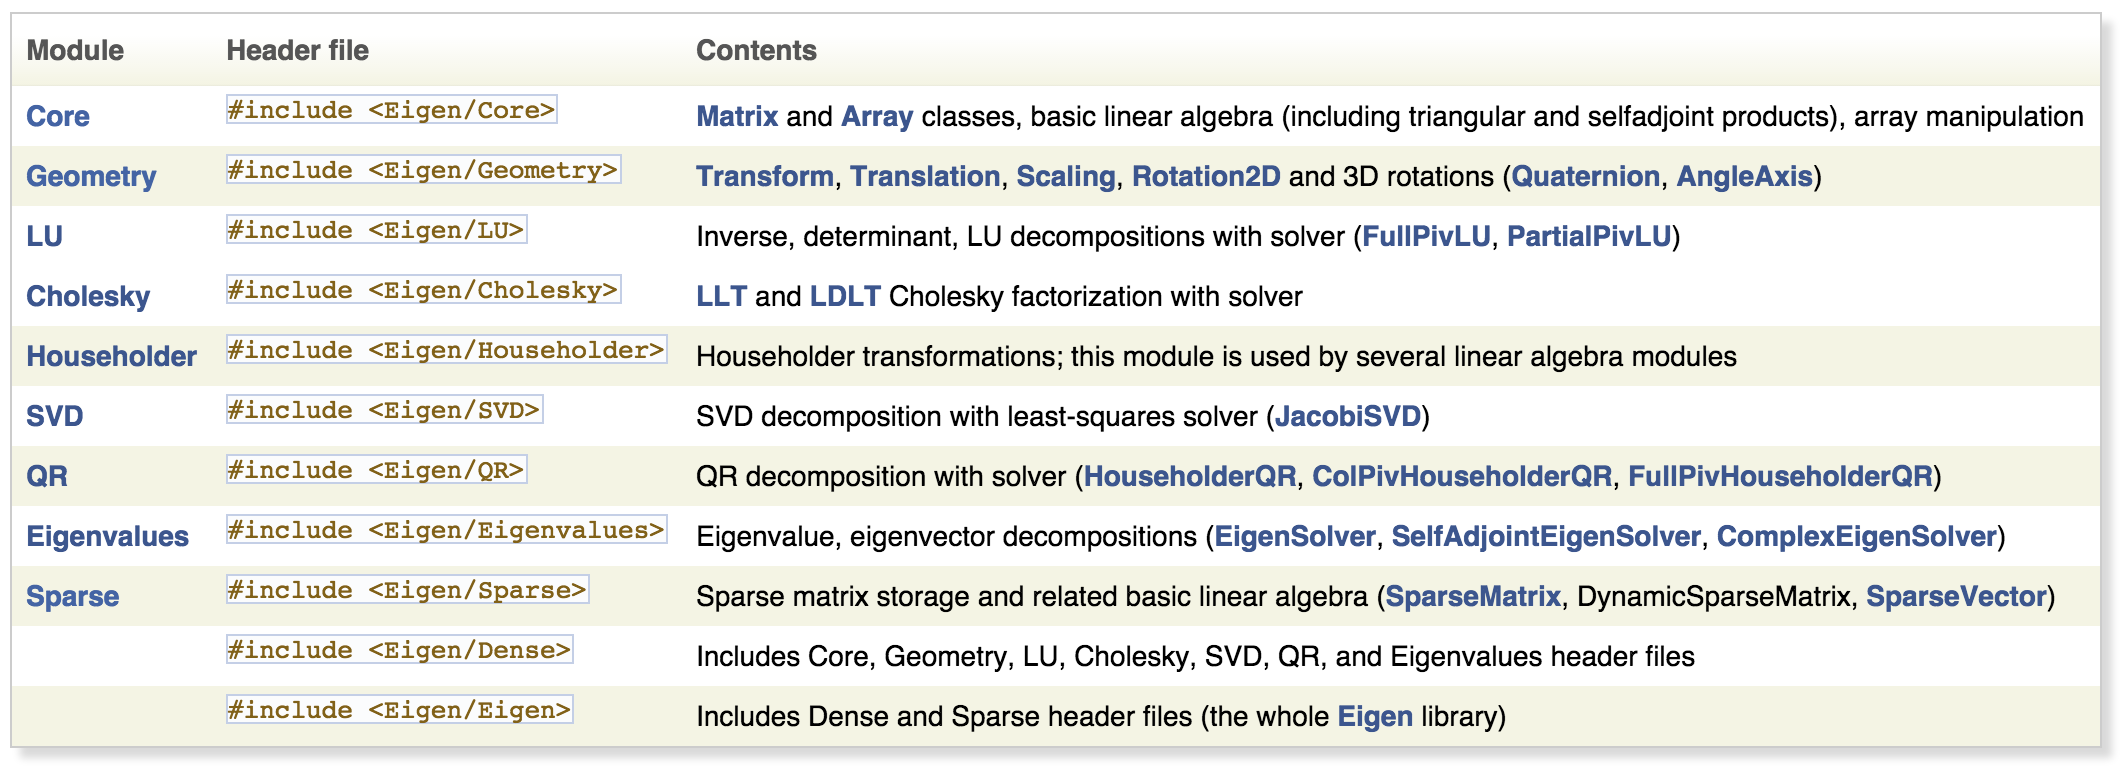
\includegraphics{03libraries/figures/eigenContents.png}
  \end{itemize}
\end{itemize}

\subsubsection{Tutorials}\label{tutorials}

Obviously, you can read:

\begin{itemize}
\itemsep1pt\parskip0pt\parsep0pt
\item
  the existing \href{http://eigen.tuxfamily.org/dox/index.html}{manual
  pages}
\item
  tutorials
  (\href{http://eigen.tuxfamily.org/dox/GettingStarted.html}{short},
  \href{http://eigen.tuxfamily.org/dox/group__TutorialMatrixClass.html}{long}).
\item
  the
  \href{http://eigen.tuxfamily.org/dox/group__QuickRefPage.html}{Quick
  Reference}
\end{itemize}

\subsubsection{Getting started}\label{getting-started}

\begin{itemize}
\itemsep1pt\parskip0pt\parsep0pt
\item
  Header only, just need \texttt{\#include}
\item
  Uses CMake, but that's just for

  \begin{itemize}
  \itemsep1pt\parskip0pt\parsep0pt
  \item
    documentation
  \item
    run unit tests
  \item
    do installation.
  \end{itemize}
\end{itemize}

\subsubsection{C++ Principles}\label{c-principles}

(i.e.~why introduce Eigen on this course)

\begin{itemize}
\itemsep1pt\parskip0pt\parsep0pt
\item
  Eigen uses

  \begin{itemize}
  \itemsep1pt\parskip0pt\parsep0pt
  \item
    Templates
  \item
    Loop unrolling, traits, template meta programming
  \end{itemize}
\end{itemize}

\subsubsection{Matrix Class}\label{matrix-class}

\begin{itemize}
\itemsep1pt\parskip0pt\parsep0pt
\item
  This:
\end{itemize}

\begin{Shaded}
\begin{Highlighting}[]
\OtherTok{#include <iostream>}
\OtherTok{#include <Eigen/Dense>}
\KeywordTok{using} \NormalTok{Eigen::MatrixXd;}
\DataTypeTok{int} \NormalTok{main()}
\NormalTok{\{}
  \NormalTok{MatrixXd m(}\DecValTok{2}\NormalTok{,}\DecValTok{2}\NormalTok{);}
  \NormalTok{m(}\DecValTok{0}\NormalTok{,}\DecValTok{0}\NormalTok{) = }\DecValTok{3}\NormalTok{;}
  \NormalTok{m(}\DecValTok{1}\NormalTok{,}\DecValTok{0}\NormalTok{) = }\FloatTok{2.5}\NormalTok{;}
  \NormalTok{m(}\DecValTok{0}\NormalTok{,}\DecValTok{1}\NormalTok{) = -}\DecValTok{1}\NormalTok{;}
  \NormalTok{m(}\DecValTok{1}\NormalTok{,}\DecValTok{1}\NormalTok{) = m(}\DecValTok{1}\NormalTok{,}\DecValTok{0}\NormalTok{) + m(}\DecValTok{0}\NormalTok{,}\DecValTok{1}\NormalTok{);}
  \NormalTok{std::cout << m << std::endl;}
\NormalTok{\}}
\end{Highlighting}
\end{Shaded}

\begin{itemize}
\itemsep1pt\parskip0pt\parsep0pt
\item
  Produces:
\end{itemize}

\begin{verbatim}
  3  -1
2.5 1.5
\end{verbatim}

\subsubsection{Matrix Class Declaration}\label{matrix-class-declaration}

Matrix Class

\begin{Shaded}
\begin{Highlighting}[]
\KeywordTok{template}\NormalTok{<}\KeywordTok{typename} \NormalTok{_Scalar, }\DataTypeTok{int} \NormalTok{_Rows, }\DataTypeTok{int} \NormalTok{_Cols, }\DataTypeTok{int} \NormalTok{_Options, }\DataTypeTok{int} \NormalTok{_MaxRows, }\DataTypeTok{int} \NormalTok{_MaxCols>}
\KeywordTok{class} \NormalTok{Matrix}
  \NormalTok{: }\KeywordTok{public} \NormalTok{PlainObjectBase<Matrix<_Scalar, _Rows, _Cols, _Options, _MaxRows, _MaxCols> >}
\NormalTok{\{}
\end{Highlighting}
\end{Shaded}

So, its templates,
\href{http://development.rc.ucl.ac.uk/training/rcwithcpp/session02/}{so
review last weeks lecture}.

\subsubsection{Matrix Class
Construction}\label{matrix-class-construction}

But in documentation:

\begin{figure}[htbp]
\centering
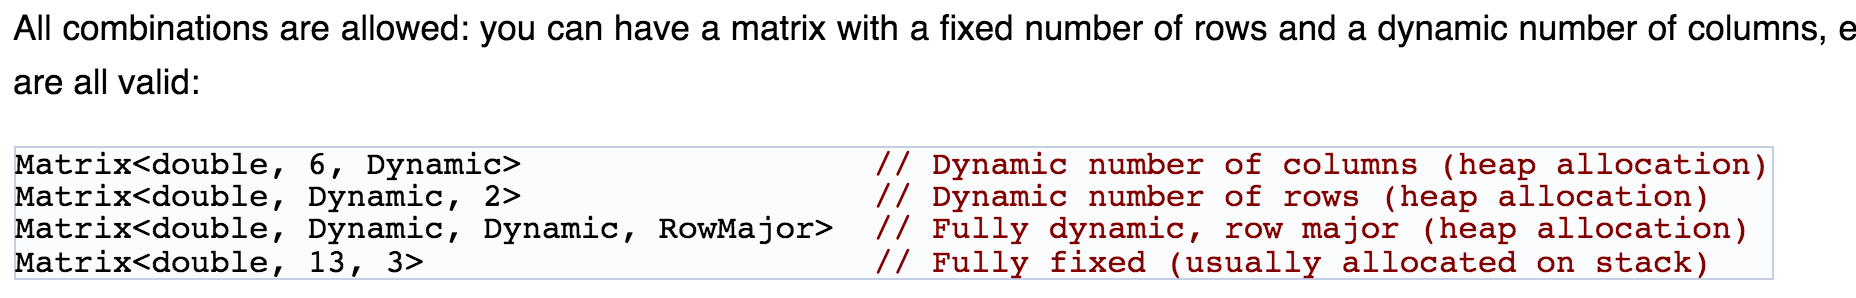
\includegraphics{03libraries/figures/eigenMatrixDynamic.png}
\caption{Matrix construction}
\end{figure}

It took a while but I searched and found:

\begin{Shaded}
\begin{Highlighting}[]
\NormalTok{src/Core/util/Constants.h:}\DataTypeTok{const} \DataTypeTok{int} \NormalTok{Dynamic = -}\DecValTok{1}\NormalTok{;}
\end{Highlighting}
\end{Shaded}

and both fixed and dynamic Matrices come from same template class???

How do they do that?

\subsubsection{DenseStorage.h - 1}\label{densestorage.h---1}

In \texttt{src/Core/DenseStorage.h}:

\begin{Shaded}
\begin{Highlighting}[]
\KeywordTok{template} \NormalTok{<}\KeywordTok{typename} \NormalTok{T, }\DataTypeTok{int} \NormalTok{Size, }\DataTypeTok{int} \NormalTok{MatrixOrArrayOptions,}
          \DataTypeTok{int} \NormalTok{Alignment = (MatrixOrArrayOptions&DontAlign) ? }\DecValTok{0}
                        \NormalTok{: (((Size*}\KeywordTok{sizeof}\NormalTok{(T))%}\DecValTok{16}\NormalTok{)==}\DecValTok{0}\NormalTok{) ? }\DecValTok{16}
                        \NormalTok{: }\DecValTok{0} \NormalTok{>}
\KeywordTok{struct} \NormalTok{plain_array}
\NormalTok{\{}
  \NormalTok{T array[Size];}
\end{Highlighting}
\end{Shaded}

So, a \texttt{plain\_array} structure containing a stack allocated
array.

\subsubsection{DenseStorage.h - 2}\label{densestorage.h---2}

In \texttt{src/Core/DenseStorage.h}:

\begin{Shaded}
\begin{Highlighting}[]
\CommentTok{// purely fixed-size matrix}
\KeywordTok{template}\NormalTok{<}\KeywordTok{typename} \NormalTok{T, }\DataTypeTok{int} \NormalTok{Size, }\DataTypeTok{int} \NormalTok{_Rows, }\DataTypeTok{int} \NormalTok{_Cols, }\DataTypeTok{int} \NormalTok{_Options> }\KeywordTok{class} \NormalTok{DenseStorage}
\NormalTok{\{}
    \NormalTok{internal::plain_array<T,Size,_Options> m_data;}
\end{Highlighting}
\end{Shaded}

There is a default template class for DenseStorage, and specialisation
for fixed arrays.

\subsubsection{DenseStorage.h - 3}\label{densestorage.h---3}

In \texttt{src/Core/DenseStorage.h}:

\begin{Shaded}
\begin{Highlighting}[]

\CommentTok{// purely dynamic matrix.}
\KeywordTok{template}\NormalTok{<}\KeywordTok{typename} \NormalTok{T, }\DataTypeTok{int} \NormalTok{_Options> }\KeywordTok{class} \NormalTok{DenseStorage<T, Dynamic, Dynamic, Dynamic, _Options>}
\NormalTok{\{}
    \NormalTok{T *m_data;}
    \NormalTok{DenseIndex m_rows;}
    \NormalTok{DenseIndex m_cols;}
\end{Highlighting}
\end{Shaded}

There is a default template class for DenseStorage, and specialisation
for Dynamic arrays.

\subsubsection{Eigen Matrix Summary}\label{eigen-matrix-summary}

\begin{itemize}
\itemsep1pt\parskip0pt\parsep0pt
\item
  Templated type supports dynamic and fixed arrays seamlessly on stack
  or heap
\item
  typedef's to make life easier: \texttt{Matrix3d} = 3 by 3 of double
\item
  Uses TMP to generate generate code at compile time
\item
  Benefit from optimisations such as loop unrolling when using fixed
  size constant arrays
\end{itemize}

\subsubsection{Eigen Usage - CMake
Include}\label{eigen-usage---cmake-include}

\begin{itemize}
\itemsep1pt\parskip0pt\parsep0pt
\item
  Need to set include path
\item
  You could download and `install' eigen into your project, and commit
  it. e.g.
\end{itemize}

\begin{Shaded}
\begin{Highlighting}[]
\KeywordTok{include_directories}\NormalTok{(}\DecValTok{$\{CMAKE_SOURCE_DIR\}}\NormalTok{/session03/cpp/Eigen/eigen-3.2.3/include/eigen3)}
\end{Highlighting}
\end{Shaded}

\subsubsection{Eigen Usage - CMake
Module}\label{eigen-usage---cmake-module}

\begin{itemize}
\itemsep1pt\parskip0pt\parsep0pt
\item
  CMake (3.1) does not have a \texttt{Find Module} for eigen, but eigen
  provides one.
\item
  So, in your source tree
\end{itemize}

\begin{Shaded}
\begin{Highlighting}[]
\KeywordTok{mkdir} \NormalTok{CMake}
\KeywordTok{cp} \KeywordTok{<}\NormalTok{path_to_eigen}\KeywordTok{>}\NormalTok{/cmake/FindEigen3.cmake ./CMake}
\end{Highlighting}
\end{Shaded}

\begin{itemize}
\itemsep1pt\parskip0pt\parsep0pt
\item
  Then in your CMakeLists.txt
\end{itemize}

\begin{Shaded}
\begin{Highlighting}[]
\KeywordTok{set}\NormalTok{(}\DecValTok{CMAKE_MODULE_PATH} \StringTok{"}\DecValTok{$\{CMAKE_SOURCE_DIR\}}\StringTok{/CMake;}\DecValTok{$\{CMAKE_MODULE_PATH\}}\StringTok{"}\NormalTok{)}
\KeywordTok{find_package}\NormalTok{(Eigen3)}
\KeywordTok{include_directories}\NormalTok{(}\DecValTok{$\{EIGEN3_INCLUDE_DIR\}}\NormalTok{)}
\end{Highlighting}
\end{Shaded}

\subsubsection{Eigen Usage - CMake
External}\label{eigen-usage---cmake-external}

\begin{itemize}
\itemsep1pt\parskip0pt\parsep0pt
\item
  \href{http://sourceforge.net/projects/niftyseg/}{NiftySeg} uses
\end{itemize}

\begin{Shaded}
\begin{Highlighting}[]
\KeywordTok{option}\NormalTok{(USE_SYSTEM_EIGEN }\StringTok{"Use an already installed version of the Eigen library"} \NormalTok{OFF)}
\KeywordTok{if}\NormalTok{(USE_SYSTEM_EIGEN)}
  \KeywordTok{find_package}\NormalTok{(EIGEN }\OtherTok{REQUIRED}\NormalTok{)}
\KeywordTok{else}\NormalTok{()}
  \KeywordTok{set}\NormalTok{(}\DecValTok{$\{PROJECT_NAME\}}\NormalTok{_VERSION_EIGEN }\StringTok{"ffa86ffb5570"} \OtherTok{CACHE} \OtherTok{STRING} \StringTok{"Version of EIGEN"} \OtherTok{FORCE}\NormalTok{)}
  \KeywordTok{set}\NormalTok{(}\DecValTok{$\{PROJECT_NAME\}}\NormalTok{_MD5_SUM_EIGEN 9559c34af203dde5f3f1d976d859c5b3 }\OtherTok{CACHE} \OtherTok{STRING} \StringTok{"MD5 check sum for EIGEN"} \OtherTok{FORCE}\NormalTok{)}
  \KeywordTok{set}\NormalTok{(}\DecValTok{$\{PROJECT_NAME\}}\NormalTok{_LOCATION_EIGEN}
    \StringTok{"http://cmic.cs.ucl.ac.uk/platform/dependencies/eigen-eigen-}\DecValTok{$\{$\{PROJECT_NAME\}_VERSION_EIGEN\}}\StringTok{.tar.gz"}
    \OtherTok{CACHE} \OtherTok{STRING} \StringTok{"Location of Eigen"} \OtherTok{FORCE}\NormalTok{)}
  \FunctionTok{ExternalProject_Add}\NormalTok{(Eigen}
    \NormalTok{URL }\DecValTok{$\{$\{PROJECT_NAME\}_LOCATION_EIGEN\}}
    \NormalTok{URL_MD5 }\DecValTok{$\{$\{PROJECT_NAME\}_MD5_SUM_EIGEN\}}
    \NormalTok{PREFIX }\DecValTok{$\{PROJECT_BINARY_DIR\}}\NormalTok{/Eigen}
    \NormalTok{DOWNLOAD_DIR }\DecValTok{$\{PROJECT_BINARY_DIR\}}\NormalTok{/Eigen/download}
    \NormalTok{SOURCE_DIR }\DecValTok{$\{PROJECT_BINARY_DIR\}}\NormalTok{/Eigen/source}
    \NormalTok{STAMP_DIR }\DecValTok{$\{PROJECT_BINARY_DIR\}}\NormalTok{/Eigen/stamps}
    \NormalTok{TMP_DIR }\DecValTok{$\{PROJECT_BINARY_DIR\}}\NormalTok{/Eigen/tmp}
    \NormalTok{BINARY_DIR }\DecValTok{$\{PROJECT_BINARY_DIR\}}\NormalTok{/Eigen/build}
    \NormalTok{CMAKE_ARGS}
      \DecValTok{$\{CMAKE_PROPAGATED_VARIABLES\}}
      \NormalTok{-DCMAKE_INSTALL_PREFIX:PATH=}\DecValTok{$\{PROJECT_BINARY_DIR\}}\NormalTok{/Eigen/install}
      \NormalTok{-DBUILD_TESTING=1}
    \NormalTok{)}
  \KeywordTok{set}\NormalTok{(Eigen_INCLUDE_DIR }\DecValTok{$\{PROJECT_BINARY_DIR\}}\NormalTok{/Eigen/install/include/eigen3)}
\KeywordTok{endif}\NormalTok{()}
\KeywordTok{include_directories}\NormalTok{(}\DecValTok{$\{Eigen_INCLUDE_DIR\}}\NormalTok{)}
\end{Highlighting}
\end{Shaded}

\subsubsection{Eigen Example - in PCL}\label{eigen-example---in-pcl}

\href{http://pointclouds.org/}{Point Cloud Library} uses
\href{http://eigen.tuxfamily.org}{Eigen}. Lets look at point based
registration of two, same length, point sets.

\subsubsection{PCL - Manual
Registration}\label{pcl---manual-registration}

\begin{itemize}
\itemsep1pt\parskip0pt\parsep0pt
\item
  Class to hold point lists
\item
  Callbacks (not shown here) to add points to list
\end{itemize}

\begin{Shaded}
\begin{Highlighting}[]
\KeywordTok{class} \NormalTok{ManualRegistration : }\KeywordTok{public} \NormalTok{QMainWindow}
\NormalTok{\{}
  \KeywordTok{protected}\NormalTok{:}
  \NormalTok{pcl::PointCloud<pcl::PointXYZ>    src_pc_;}
  \NormalTok{pcl::PointCloud<pcl::PointXYZ>    dst_pc_;}
  \NormalTok{Eigen::Matrix4f                   transform_;  }
\end{Highlighting}
\end{Shaded}

\subsubsection{PCL - SVD class}\label{pcl---svd-class}

\begin{itemize}
\itemsep1pt\parskip0pt\parsep0pt
\item
  In \texttt{apps/src/manual\_registration/manual\_registration.cpp}
\item
  Create a class to estimate SVD of two point sets
\item
  See paper \href{http://dl.acm.org/citation.cfm?id=28821}{Arun et. al.
  1987}
\item
  Its an example of the orthogonal procrustes problem
\end{itemize}

\begin{Shaded}
\begin{Highlighting}[]
  \NormalTok{pcl::registration::TransformationEstimationSVD<pcl::PointXYZ, pcl::PointXYZ> tfe;}
  \NormalTok{tfe.estimateRigidTransformation(src_pc_, dst_pc_, transform_);}
\end{Highlighting}
\end{Shaded}

\subsubsection{PCL - Correlation}\label{pcl---correlation}

After subtracting each point from the mean point we have in
\texttt{registration/include/pcl/registration/impl/transformation\_estimation\_svd.hpp}

\begin{Shaded}
\begin{Highlighting}[]
\KeywordTok{template} \NormalTok{<}\KeywordTok{typename} \NormalTok{PointSource, }\KeywordTok{typename} \NormalTok{PointTarget, }\KeywordTok{typename} \NormalTok{Scalar> }\DataTypeTok{void}
\NormalTok{pcl::registration::TransformationEstimationSVD<PointSource, PointTarget, Scalar>::getTransformationFromCorrelation (}
    \DataTypeTok{const} \NormalTok{Eigen::Matrix<Scalar, Eigen::Dynamic, Eigen::Dynamic> &cloud_src_demean,}
    \DataTypeTok{const} \NormalTok{Eigen::Matrix<Scalar, }\DecValTok{4}\NormalTok{, }\DecValTok{1}\NormalTok{> &centroid_src,}
    \DataTypeTok{const} \NormalTok{Eigen::Matrix<Scalar, Eigen::Dynamic, Eigen::Dynamic> &cloud_tgt_demean,}
    \DataTypeTok{const} \NormalTok{Eigen::Matrix<Scalar, }\DecValTok{4}\NormalTok{, }\DecValTok{1}\NormalTok{> &centroid_tgt,}
    \NormalTok{Matrix4 &transformation_matrix) }\DataTypeTok{const}
\NormalTok{\{}
  \NormalTok{transformation_matrix.setIdentity ();}

  \CommentTok{// Assemble the correlation matrix H = source * target'}
  \NormalTok{Eigen::Matrix<Scalar, }\DecValTok{3}\NormalTok{, }\DecValTok{3}\NormalTok{> H = (cloud_src_demean * cloud_tgt_demean.transpose ()).topLeftCorner (}\DecValTok{3}\NormalTok{, }\DecValTok{3}\NormalTok{);}

  \CommentTok{// Compute the Singular Value Decomposition}
  \NormalTok{Eigen::JacobiSVD<Eigen::Matrix<Scalar, }\DecValTok{3}\NormalTok{, }\DecValTok{3}\NormalTok{> > svd (H, Eigen::ComputeFullU | Eigen::ComputeFullV);}
  \NormalTok{Eigen::Matrix<Scalar, }\DecValTok{3}\NormalTok{, }\DecValTok{3}\NormalTok{> u = svd.matrixU ();}
  \NormalTok{Eigen::Matrix<Scalar, }\DecValTok{3}\NormalTok{, }\DecValTok{3}\NormalTok{> v = svd.matrixV ();}

  \CommentTok{// Compute R = V * U'}
  \KeywordTok{if} \NormalTok{(u.determinant () * v.determinant () < }\DecValTok{0}\NormalTok{)}
  \NormalTok{\{}
    \KeywordTok{for} \NormalTok{(}\DataTypeTok{int} \NormalTok{x = }\DecValTok{0}\NormalTok{; x < }\DecValTok{3}\NormalTok{; ++x)}
      \NormalTok{v (x, }\DecValTok{2}\NormalTok{) *= -}\DecValTok{1}\NormalTok{;}
  \NormalTok{\}}

  \NormalTok{Eigen::Matrix<Scalar, }\DecValTok{3}\NormalTok{, }\DecValTok{3}\NormalTok{> R = v * u.transpose ();}

  \CommentTok{// Return the correct transformation}
  \NormalTok{transformation_matrix.topLeftCorner (}\DecValTok{3}\NormalTok{, }\DecValTok{3}\NormalTok{) = R;}
  \DataTypeTok{const} \NormalTok{Eigen::Matrix<Scalar, }\DecValTok{3}\NormalTok{, }\DecValTok{1}\NormalTok{> Rc (R * centroid_src.head (}\DecValTok{3}\NormalTok{));}
  \NormalTok{transformation_matrix.block (}\DecValTok{0}\NormalTok{, }\DecValTok{3}\NormalTok{, }\DecValTok{3}\NormalTok{, }\DecValTok{1}\NormalTok{) = centroid_tgt.head (}\DecValTok{3}\NormalTok{) - Rc;}
\NormalTok{\}}
\end{Highlighting}
\end{Shaded}

\subsubsection{PCL - Summary}\label{pcl---summary}

\begin{itemize}
\itemsep1pt\parskip0pt\parsep0pt
\item
  Use of Eigen implements
  \href{http://dl.acm.org/citation.cfm?id=28821}{Arun et. al. 1987} in
  one main function.
\item
  Relatively close matching of algorithm to code.
\item
  Template notation a bit awkward, but now, not so insurmountable.
\item
  So, using library, we gain power and benefit of very experienced
  library programmers.
\end{itemize}

\subsubsection{Eigen Summary}\label{eigen-summary}

\begin{itemize}
\itemsep1pt\parskip0pt\parsep0pt
\item
  Header only
\item
  Use CMake to set the include path
\item
  Templated, so its compiled in, no link or run-time dependencies
\item
  Simple to use linear algebra library
\item
  Advise not to mix with GUI code
\item
  Consider static linking as using templates anyway - ease of
  distribution
\end{itemize}

\subsection{Using Boost}\label{using-boost}

\subsubsection{Introduction}\label{introduction-1}

\begin{itemize}
\itemsep1pt\parskip0pt\parsep0pt
\item
  \href{http://www.boost.org}{Boost} is ``\ldots{}one of the most highly
  regarded and expertly designed C++ library projects in the world.''
\item
  A \href{http://www.boost.org/doc/libs/1_57_0/}{large (121+)}
  collection of C++ libraries
\item
  Aim to establish standards, contribute to C++11, C++17 etc.
\item
  Hard to use C++ without bumping into Boost at some point
\item
  It's heavily templated
\item
  Many libraries header only, some require compiling.
\end{itemize}

\subsubsection{Libraries included}\label{libraries-included}

\begin{itemize}
\itemsep1pt\parskip0pt\parsep0pt
\item
  Log, FileSystem, Asio, Serialization, Pool (memory) \ldots{}
\item
  Regexp, String Algo, DateTime, \ldots{}
\item
  Math, Odeint, Graph, Polygon, Rational, \ldots{}
\item
  Each has good documentation, and tutorial, and unit tests, and is
  widely compiled.
\end{itemize}

\subsubsection{Getting started}\label{getting-started-1}

\begin{itemize}
\itemsep1pt\parskip0pt\parsep0pt
\item
  Default build system: \texttt{bjam}
\item
  Also CMake version of boost project, possible deprecated.
\item
  Once installed, many header only libraries, so similar to Eigen.
\end{itemize}

\subsubsection{Installing pre-compiled}\label{installing-pre-compiled}

\begin{itemize}
\itemsep1pt\parskip0pt\parsep0pt
\item
  Linux:

  \begin{itemize}
  \itemsep1pt\parskip0pt\parsep0pt
  \item
    \texttt{sudo apt-get install boost}
  \item
    \texttt{sudo apt-get install libboost1.53-dev}
  \end{itemize}
\item
  Mac

  \begin{itemize}
  \itemsep1pt\parskip0pt\parsep0pt
  \item
    Homebrew (brew) or Macports (port)
  \end{itemize}
\item
  Windows

  \begin{itemize}
  \itemsep1pt\parskip0pt\parsep0pt
  \item
    Precompiled binaries? Probably you need to build from source.
  \end{itemize}
\end{itemize}

\subsubsection{Compiling from source}\label{compiling-from-source}

\begin{itemize}
\itemsep1pt\parskip0pt\parsep0pt
\item
  \href{http://www.boost.org/doc/libs/1_57_0/libs/regex/doc/html/boost_regex/install.html}{Follow
  build instructions here}
\item
  Or use bigger project with it as part of build system

  \begin{itemize}
  \itemsep1pt\parskip0pt\parsep0pt
  \item
    NifTK, MITK, Slicer, Gimias (medical imaging)
  \end{itemize}
\end{itemize}

\subsubsection{C++ Principles}\label{c-principles-1}

(i.e.~why introduce Boost on this course)

\begin{itemize}
\itemsep1pt\parskip0pt\parsep0pt
\item
  Boost uses

  \begin{itemize}
  \itemsep1pt\parskip0pt\parsep0pt
  \item
    Templates
  \item
    Widespread use of:

    \begin{itemize}
    \itemsep1pt\parskip0pt\parsep0pt
    \item
      Generic Programming
    \item
      Template Meta-Programming
    \end{itemize}
  \item
    Functors
  \end{itemize}
\end{itemize}

\subsubsection{C Function Pointers - 1}\label{c-function-pointers---1}

\begin{itemize}
\itemsep1pt\parskip0pt\parsep0pt
\item
  Useful if using \href{http://www.nr.com/}{Numerical Recipes in C}
\item
  See \href{http://en.wikipedia.org/wiki/Function_pointer}{Wikipedia}
  article and tutorials online
\end{itemize}

This:

\begin{Shaded}
\begin{Highlighting}[]
\OtherTok{#include <stdio.h>  }\CommentTok{/* for printf */}
\DataTypeTok{double} \NormalTok{cm_to_inches(}\DataTypeTok{double} \NormalTok{cm) \{}
  \KeywordTok{return} \NormalTok{cm / }\FloatTok{2.54}\NormalTok{;}
\NormalTok{\}}
\DataTypeTok{int} \NormalTok{main(}\DataTypeTok{void}\NormalTok{) \{}
  \DataTypeTok{double} \NormalTok{(*func1)(}\DataTypeTok{double}\NormalTok{)            = cm_to_inches;}
  \NormalTok{printf(}\StringTok{"Converting %f cm to %f inches by calling function.}\CharTok{\textbackslash{}n}\StringTok{"}\NormalTok{, }\FloatTok{5.0}\NormalTok{, cm_to_inches(}\FloatTok{5.0}\NormalTok{));}
  \NormalTok{printf(}\StringTok{"Converting %f cm to %f inches by deref pointer.}\CharTok{\textbackslash{}n}\StringTok{"}\NormalTok{, }\FloatTok{15.0}\NormalTok{, func1(}\FloatTok{15.0}\NormalTok{));}
  \KeywordTok{return} \DecValTok{0}\NormalTok{;}
\NormalTok{\}}
\end{Highlighting}
\end{Shaded}

Produces:

\begin{verbatim}
Converting 5.000000 cm to 1.968504 inches by calling function.
Converting 15.000000 cm to 5.905512 inches by deref pointer.
\end{verbatim}

\subsubsection{C Function Pointers - 2}\label{c-function-pointers---2}

\begin{itemize}
\itemsep1pt\parskip0pt\parsep0pt
\item
  Function pointers can be passed to functions
\end{itemize}

This:

\begin{Shaded}
\begin{Highlighting}[]
\OtherTok{#include <stdio.h>  }
\OtherTok{#include <math.h>  }
\DataTypeTok{double} \NormalTok{integrate(}\DataTypeTok{double} \NormalTok{(*funcp)(}\DataTypeTok{double}\NormalTok{), }\DataTypeTok{double} \NormalTok{lo, }\DataTypeTok{double} \NormalTok{hi) \{}
  \DataTypeTok{double}  \NormalTok{sum = }\FloatTok{0.0}\NormalTok{;}
  \KeywordTok{for} \NormalTok{(}\DataTypeTok{int} \NormalTok{i = }\DecValTok{0}\NormalTok{;  i <= }\DecValTok{100}\NormalTok{;  i++)}
  \NormalTok{\{}
    \NormalTok{sum += (*funcp)(i / }\FloatTok{100.0} \NormalTok{* (hi - lo) + lo);}
  \NormalTok{\}}
  \KeywordTok{return} \NormalTok{sum / }\FloatTok{100.0}\NormalTok{;}
\NormalTok{\}}
\DataTypeTok{int} \NormalTok{main(}\DataTypeTok{void}\NormalTok{) \{}
  \DataTypeTok{double}  \NormalTok{(*fp)(}\DataTypeTok{double}\NormalTok{) = sin;}
  \NormalTok{printf(}\StringTok{"sum(sin): %f}\CharTok{\textbackslash{}n}\StringTok{"}\NormalTok{, integrate(fp, }\FloatTok{0.0}\NormalTok{, }\FloatTok{1.0}\NormalTok{));}
  \KeywordTok{return} \DecValTok{0}\NormalTok{;}
\NormalTok{\}}
\end{Highlighting}
\end{Shaded}

Produces:

\begin{verbatim}
sum(sin): 0.463901
\end{verbatim}

\subsubsection{C Function Pointers - 3}\label{c-function-pointers---3}

\begin{itemize}
\itemsep1pt\parskip0pt\parsep0pt
\item
  Function pointers

  \begin{itemize}
  \itemsep1pt\parskip0pt\parsep0pt
  \item
    often used for callbacks, cost functions in optimisation etc.
  \item
    called by name, or dereference pointer
  \item
    are generally stateless
  \end{itemize}
\end{itemize}

\subsubsection{C++ Function Objects - 1}\label{c-function-objects---1}

\begin{itemize}
\itemsep1pt\parskip0pt\parsep0pt
\item
  We can define an object to represent a function

  \begin{itemize}
  \itemsep1pt\parskip0pt\parsep0pt
  \item
    Called \href{http://en.wikipedia.org/wiki/Function_object}{Function
    Object} or Functor
  \end{itemize}
\end{itemize}

This:

\begin{Shaded}
\begin{Highlighting}[]
\OtherTok{#include <vector>}
\OtherTok{#include <algorithm>}
\OtherTok{#include <iostream>}
\KeywordTok{struct} \NormalTok{IntComparator}
\NormalTok{\{}
  \DataTypeTok{bool} \KeywordTok{operator}\NormalTok{()(}\DataTypeTok{const} \DataTypeTok{int} \NormalTok{&a, }\DataTypeTok{const} \DataTypeTok{int} \NormalTok{&b) }\DataTypeTok{const}
  \NormalTok{\{}
    \KeywordTok{return} \NormalTok{a < b;}
  \NormalTok{\}}
\NormalTok{\};}
\CommentTok{/*}
\CommentTok{template <class RandomIt, class Compare>}
\CommentTok{void sort(RandomIt first, RandomIt last, Compare comp);}
\CommentTok{*/}
\DataTypeTok{int} \NormalTok{main()}
\NormalTok{\{}
    \NormalTok{std::vector<}\DataTypeTok{int}\NormalTok{> items;}
    \NormalTok{items.push_back(}\DecValTok{1}\NormalTok{);}
    \NormalTok{items.push_back(}\DecValTok{3}\NormalTok{);}
    \NormalTok{items.push_back(}\DecValTok{2}\NormalTok{);}
    \NormalTok{std::sort(items.begin(), items.end(), IntComparator());}
    \NormalTok{std::cout << items[}\DecValTok{0}\NormalTok{] << }\StringTok{","} \NormalTok{<< items[}\DecValTok{1}\NormalTok{] << }\StringTok{","} \NormalTok{<< items[}\DecValTok{2}\NormalTok{] << std::endl;}
    \KeywordTok{return} \DecValTok{0}\NormalTok{;}
\NormalTok{\}}
\end{Highlighting}
\end{Shaded}

Produces:

\begin{verbatim}
1,2,3
\end{verbatim}

\subsubsection{C++ Function Objects - 2}\label{c-function-objects---2}

\begin{itemize}
\itemsep1pt\parskip0pt\parsep0pt
\item
  But function objects can

  \begin{itemize}
  \itemsep1pt\parskip0pt\parsep0pt
  \item
    Have state
  \item
    Have member variables
  \item
    Be complex objects, created by any means
  \item
    e.g.~Cost function, similarity between two images
  \end{itemize}
\end{itemize}

\subsubsection{CMake for Boost}\label{cmake-for-boost}

\begin{itemize}
\itemsep1pt\parskip0pt\parsep0pt
\item
  If installed correctly, should be something like:
\end{itemize}

\begin{verbatim}
set(Boost_ADDITIONAL_VERSIONS 1.53.0 1.54.0 1.53 1.54)
find_package(Boost 1.53.0)
if(Boost_FOUND)
    include_directories(${Boost_INCLUDE_DIRS})
endif()
\end{verbatim}

\subsubsection{Boost Example}\label{boost-example}

\begin{itemize}
\itemsep1pt\parskip0pt\parsep0pt
\item
  With 121+ libraries, can't give tutorial on each one!
\item
  Pick one small numerical example
\item
  Illustrate the use of functors in ODE integration
\end{itemize}

\subsubsection{Using Boost odeint}\label{using-boost-odeint}

\begin{itemize}
\itemsep1pt\parskip0pt\parsep0pt
\item
  Its a numerical example, as we are doing scientific computing!
\item
  As with many libraries, just include right header
\end{itemize}

\begin{verbatim}
#include <boost/numeric/odeint.hpp> // Include ODE solver library
                                    // just to check our build system found it
\end{verbatim}

\begin{itemize}
\itemsep1pt\parskip0pt\parsep0pt
\item
  See
  \href{http://www.boost.org/doc/libs/1_57_0/libs/type_traits/doc/html/boost_typetraits/background.html}{this
  tutorial}
\end{itemize}

\subsubsection{Boost odeint - 1}\label{boost-odeint---1}

Given these global definitions:

\begin{Shaded}
\begin{Highlighting}[]

\DataTypeTok{const} \DataTypeTok{double} \NormalTok{gam = }\FloatTok{0.15}\NormalTok{;}
\KeywordTok{typedef} \NormalTok{std::vector< }\DataTypeTok{double} \NormalTok{> state_type;}

\CommentTok{// This is functor class}
\end{Highlighting}
\end{Shaded}

\subsubsection{Boost odeint - 2}\label{boost-odeint---2}

First define a functor for the function to integrate:

\begin{Shaded}
\begin{Highlighting}[]

\KeywordTok{class} \NormalTok{harm_osc \{}
    \DataTypeTok{double} \NormalTok{m_gam; }\CommentTok{// class can have member variables, state etc.}
\KeywordTok{public}\NormalTok{:}
    \NormalTok{harm_osc( }\DataTypeTok{double} \NormalTok{gam ) : m_gam(gam) \{ \}}

    \CommentTok{// odeint integrators normally call f(x, dxdt, t)}
    \DataTypeTok{void} \KeywordTok{operator}\NormalTok{() ( }\DataTypeTok{const} \NormalTok{state_type &x , state_type &dxdt , }\DataTypeTok{const} \DataTypeTok{double} \CommentTok{/* t */} \NormalTok{)}
    \NormalTok{\{}
        \NormalTok{dxdt[}\DecValTok{0}\NormalTok{] = x[}\DecValTok{1}\NormalTok{];}
        \NormalTok{dxdt[}\DecValTok{1}\NormalTok{] = -x[}\DecValTok{0}\NormalTok{] - m_gam*x[}\DecValTok{1}\NormalTok{];}
    \NormalTok{\}}
\NormalTok{\};}

\CommentTok{// This is observer to record output, and is also a functor class}
\end{Highlighting}
\end{Shaded}

\subsubsection{Boost odeint - 3}\label{boost-odeint---3}

Define an observer to collect graph-points:

\begin{Shaded}
\begin{Highlighting}[]

\KeywordTok{struct} \NormalTok{push_back_state_and_time}
\NormalTok{\{}
    \NormalTok{std::vector< state_type >& m_states;}
    \NormalTok{std::vector< }\DataTypeTok{double} \NormalTok{>& m_times;}

    \NormalTok{push_back_state_and_time( std::vector< state_type > &states , std::vector< }\DataTypeTok{double} \NormalTok{> &times )}
    \NormalTok{: m_states( states ) , m_times( times ) \{ \}}

    \DataTypeTok{void} \KeywordTok{operator}\NormalTok{()( }\DataTypeTok{const} \NormalTok{state_type &x , }\DataTypeTok{double} \NormalTok{t )}
    \NormalTok{\{}
        \NormalTok{m_states.push_back( x );}
        \NormalTok{m_times.push_back( t );}
    \NormalTok{\}}
\NormalTok{\};}
\end{Highlighting}
\end{Shaded}

\subsubsection{Boost odeint - 4}\label{boost-odeint---4}

The run it:

\begin{Shaded}
\begin{Highlighting}[]

\DataTypeTok{int} \NormalTok{main(}\DataTypeTok{void}\NormalTok{) \{}

  \NormalTok{state_type x(}\DecValTok{2}\NormalTok{);}
  \NormalTok{x[}\DecValTok{0}\NormalTok{] = }\FloatTok{1.0}\NormalTok{; }\CommentTok{// start at x=1.0, p=0.0}
  \NormalTok{x[}\DecValTok{1}\NormalTok{] = }\FloatTok{0.0}\NormalTok{;}

  \NormalTok{std::vector<state_type> x_vec; }\CommentTok{// vector of vectors}
  \NormalTok{std::vector<}\DataTypeTok{double}\NormalTok{> times;     }\CommentTok{// stores each time point}

  \NormalTok{harm_osc harmonic_oscillator(}\FloatTok{0.15}\NormalTok{);}
  \NormalTok{size_t steps = boost::numeric::odeint::integrate(}
    \NormalTok{harmonic_oscillator ,}
    \NormalTok{x , }\FloatTok{0.0} \NormalTok{, }\FloatTok{10.0} \NormalTok{, }\FloatTok{0.1} \NormalTok{,}
    \NormalTok{push_back_state_and_time( x_vec , times ) );}

  \KeywordTok{for}\NormalTok{( size_t i=}\DecValTok{0}\NormalTok{; i<=steps; i++ )}
  \NormalTok{\{}
    \NormalTok{std::cout << times[i] << }\CharTok{'\textbackslash{}t'} \NormalTok{<< x_vec[i][}\DecValTok{0}\NormalTok{] << }\CharTok{'\textbackslash{}t'} \NormalTok{<< x_vec[i][}\DecValTok{1}\NormalTok{] << }\CharTok{'\textbackslash{}n'}\NormalTok{;}
  \NormalTok{\}}

\NormalTok{\}}
\end{Highlighting}
\end{Shaded}

\subsubsection{Boost odeint - 4}\label{boost-odeint---4-1}

Produces:

\begin{verbatim}
0   1   0
0.1 0.995029    -0.0990884
0.342911    0.942763    -0.32773
0.59639 0.832373    -0.537274
0.865439    0.662854    -0.714058
1.15445 0.436595    -0.839871
1.44346 0.184494    -0.892171
1.70128 -0.0446646  -0.875731
1.9591  -0.262234   -0.80313
2.21692 -0.454545   -0.681207
2.48815 -0.616993   -0.510476
2.77613 -0.733844   -0.296963
3.06411 -0.7866 -0.0685387
3.35209 -0.773719   0.155753
3.64008 -0.699015   0.358007
3.92806 -0.571123   0.522852
4.21604 -0.402601   0.638582
4.50402 -0.20875    0.697943
4.792   -0.0062679  0.698535
5.07998 0.188159    0.642795
5.36797 0.359199    0.537596
5.65595 0.494053    0.39351
5.94393 0.583381    0.223796
6.23191 0.621907    0.0432166
6.51989 0.608673    -0.133212
6.80787 0.546935    -0.291443
7.09586 0.44372 -0.419492
7.39491 0.303457    -0.510857
7.69397 0.143005    -0.553869
7.99302 -0.0228226  -0.546913
8.29208 -0.179394   -0.492786
8.59113 -0.313525   -0.398255
8.89019 -0.414555   -0.273299
9.18925 -0.475166   -0.130101
9.4883  -0.49187    0.0181101
9.78736 -0.465143   0.158247
10  -0.421907   0.246407
\end{verbatim}

\subsubsection{Why Boost for Numerics}\label{why-boost-for-numerics}

\begin{itemize}
\itemsep1pt\parskip0pt\parsep0pt
\item
  Broader question is

  \begin{itemize}
  \itemsep1pt\parskip0pt\parsep0pt
  \item
    Why someone else's library? Boost or some other.
  \end{itemize}
\item
  Advanced use of Template Meta Programming, Traits

  \begin{itemize}
  \itemsep1pt\parskip0pt\parsep0pt
  \item
    Performance optimisations
  \item
    Alternative implementations

    \begin{itemize}
    \itemsep1pt\parskip0pt\parsep0pt
    \item
      CUDA via Thrust
    \item
      MPI
    \item
      etc
    \end{itemize}
  \end{itemize}
\item
  You just focus on your bit
\end{itemize}

\subsection{Using ITK}\label{using-itk}

\subsubsection{Introduction}\label{introduction-2}

\begin{itemize}
\itemsep1pt\parskip0pt\parsep0pt
\item
  \href{http://www.itk.org}{Insight Segmentation and Registration
  Toolkit}
\item
  Insight Journal for library additions
\item
  Large community in medical image processing
\item
  Deliberately no visualisation, see \href{http://www.vtk.org}{VTK}.
\end{itemize}

\subsubsection{C++ Principles}\label{c-principles-2}

\begin{itemize}
\itemsep1pt\parskip0pt\parsep0pt
\item
  Heavy use of Generic Programming
\item
  Use of Template Meta-Programming
\item
  Often perceived by ``scientific programmers'' (Matlab) as difficult
\item
  Aim: demonstrate here, that we can now use it!
\item
  Of particular interest

  \begin{itemize}
  \itemsep1pt\parskip0pt\parsep0pt
  \item
    typedefs - make life easier
  \item
    SmartPointers - reduce leaking memory
  \item
    Iterators - fast image access
  \item
    Object Factories - extensibility
  \end{itemize}
\end{itemize}

\subsubsection{Architecture Concept}\label{architecture-concept}

\begin{itemize}
\itemsep1pt\parskip0pt\parsep0pt
\item
  Use of pipeline of filters
\item
  Simple to plug image processing filters together
\item
  Sometimes difficult to manage memory for huge images
\end{itemize}

\subsubsection{Filter Usage - 1}\label{filter-usage---1}

We work through a simple filter program. First, typedefs are aliases.

\begin{Shaded}
\begin{Highlighting}[]

\DataTypeTok{int} \NormalTok{main(}\DataTypeTok{int} \NormalTok{argc, }\DataTypeTok{char}\NormalTok{** argv)}
\NormalTok{\{}

  \DataTypeTok{const} \DataTypeTok{unsigned} \DataTypeTok{int} \NormalTok{Dimension = }\DecValTok{2}\NormalTok{;}
  \KeywordTok{typedef} \DataTypeTok{int} \NormalTok{PixelType;}
  \KeywordTok{typedef} \NormalTok{itk::Image<PixelType, Dimension> ImageType;}
  \KeywordTok{typedef} \NormalTok{itk::AddImageFilter<ImageType, ImageType> AddFilterType;}
  \KeywordTok{typedef} \NormalTok{itk::ImageFileReader<ImageType> ImageReaderType;}
  \KeywordTok{typedef} \NormalTok{itk::ImageFileWriter<ImageType> ImageWriterType;}
\end{Highlighting}
\end{Shaded}

\subsubsection{Filter Usage - 2}\label{filter-usage---2}

Objects are constructed:

\begin{Shaded}
\begin{Highlighting}[]

  \NormalTok{ImageReaderType::Pointer reader1 = ImageReaderType::New();}
  \NormalTok{ImageReaderType::Pointer reader2 = ImageReaderType::New();}
  \NormalTok{AddFilterType::Pointer addFilter = AddFilterType::New();}
  \NormalTok{ImageWriterType::Pointer writer = ImageWriterType::New();}

  \CommentTok{// eg. if not using typedefs}
  \CommentTok{//itk::ImageFileWriter< itk::Image<int, 2> >::Pointer writer}
  \CommentTok{//  = itk::ImageFileWriter< itk::Image<int, 2> >::New();}
\end{Highlighting}
\end{Shaded}

\subsubsection{Filter Usage - 3}\label{filter-usage---3}

Pipeline is executed:

\begin{Shaded}
\begin{Highlighting}[]

  \NormalTok{reader1->SetFileName(}\StringTok{"inputFileName1.nii"}\NormalTok{);}
  \NormalTok{reader2->SetFileName(}\StringTok{"inputFileName2.nii"}\NormalTok{);}
  \NormalTok{addFilter->SetInput(}\DecValTok{0}\NormalTok{, reader1->GetOutput());}
  \NormalTok{addFilter->SetInput(}\DecValTok{1}\NormalTok{, reader2->GetOutput());}
  \NormalTok{writer->SetInput(addFilter->GetOutput());}
  \NormalTok{writer->SetFileName(}\StringTok{"outputFileName1.nii"}\NormalTok{);}
  \CommentTok{//writer->Update(); // commented out, as filenames are fake.}
                      \CommentTok{// and build system for lecture notes}
                      \CommentTok{// tries to run the program.}
  \KeywordTok{return} \DecValTok{0}\NormalTok{;}
\NormalTok{\}}
\end{Highlighting}
\end{Shaded}

More information on ITK Pipeline can be found in the
\href{http://www.itk.org/ItkSoftwareGuide.pdf}{ITK Software Guide}.

\subsubsection{Smart Pointer Intro}\label{smart-pointer-intro}

Lets look at some interesting features.

\begin{itemize}
\itemsep1pt\parskip0pt\parsep0pt
\item
  Smart Pointer

  \begin{itemize}
  \itemsep1pt\parskip0pt\parsep0pt
  \item
    Class, like a pointer, but `Smarter' (clever)
  \item
    Typically, once allocated will automatically destroy the pointed to
    object
  \item
    Implementations vary, STL, ITK, VTK, Qt, so read the docs
  \end{itemize}
\item
  So, in each class e.g.~itkAddImageFilter
\end{itemize}

\begin{Shaded}
\begin{Highlighting}[]
\KeywordTok{typedef} \NormalTok{AddImageFilter     Self}
\KeywordTok{typedef} \NormalTok{SmartPointer<Self> Pointer}
\end{Highlighting}
\end{Shaded}

and so, its used like

\begin{Shaded}
\begin{Highlighting}[]
\NormalTok{ClassName::Pointer variableName = ClassName::New();}
\end{Highlighting}
\end{Shaded}

\subsubsection{Smart Pointer Class}\label{smart-pointer-class}

In the SmartPointer itself

\begin{Shaded}
\begin{Highlighting}[]
  \CommentTok{/** Constructor to pointer p  */}
  \NormalTok{SmartPointer (ObjectType *p):}
    \NormalTok{m_Pointer(p)}
  \NormalTok{\{ }\KeywordTok{this}\NormalTok{->Register(); \}}

  \CommentTok{/** Destructor  */}
  \NormalTok{~SmartPointer ()}
  \NormalTok{\{}
    \KeywordTok{this}\NormalTok{->UnRegister();}
    \NormalTok{m_Pointer = ITK_SP_NULLPTR;}
  \NormalTok{\}}
\end{Highlighting}
\end{Shaded}

and

\begin{Shaded}
\begin{Highlighting}[]
\KeywordTok{private}\NormalTok{:}
  \CommentTok{/** The pointer to the object referred to by this smart pointer. */}
  \NormalTok{ObjectType *m_Pointer;}

  \DataTypeTok{void} \NormalTok{Register()}
  \NormalTok{\{}
    \KeywordTok{if} \NormalTok{( m_Pointer ) \{ m_Pointer->Register(); \}}
  \NormalTok{\}}
\end{Highlighting}
\end{Shaded}

\subsubsection{General Smart Pointer
Usage}\label{general-smart-pointer-usage}

\begin{itemize}
\itemsep1pt\parskip0pt\parsep0pt
\item
  Avoid use of explicit pairs of \texttt{new/delete}
\item
  Immediately assign object to SmartPointer
\item
  Consistently (i.e.~always) use SmartPointer

  \begin{itemize}
  \itemsep1pt\parskip0pt\parsep0pt
  \item
    Pass (reference to) SmartPointer to function.
  \item
    Can (but should you?) return SmartPointer from function.
  \item
    Don't use raw pointer, and don't store raw pointers to objects.
  \item
    You can't test raw pointer to check if object still exists.
  \end{itemize}
\item
  Object is deleted when last SmartPointer reference goes out of scope
\end{itemize}

\subsubsection{ITK SmartPointer}\label{itk-smartpointer}

\begin{itemize}
\itemsep1pt\parskip0pt\parsep0pt
\item
  ITK keeps reference count in itk::LightObject base class
\item
  So, it can only be used by sub-classes of itk::LightObject
\item
  Reference is held in the object
\item
  Same method used in MITK, as MITK uses ITK concepts
\item
  \href{http://www.vtk.org}{VTK} has a SmartPointer that requires
  calling Delete explicitly (!!)
\item
  STL has much clearer definition of different types of smart pointer
\item
  Read
  \href{http://www.umich.edu/~eecs381/handouts/C++11_smart_ptrs.pdf}{THIS}
  tutorial
\end{itemize}

\subsubsection{Implementing a Filter}\label{implementing-a-filter}

\begin{itemize}
\itemsep1pt\parskip0pt\parsep0pt
\item
  ITK provides many image processing filters.
\item
  But you can write your own easily

  \begin{itemize}
  \itemsep1pt\parskip0pt\parsep0pt
  \item
    Single Threaded - override GenerateData()
  \item
    Multi-Threaded - override ThreadedGenerateData()
  \end{itemize}
\item
  Now we see an example - thresholding, as we want to study the C++ not
  the image processing.
\end{itemize}

\subsubsection{Filter Impl - 1}\label{filter-impl---1}

Basic filter:

\begin{Shaded}
\begin{Highlighting}[]

\KeywordTok{namespace} \NormalTok{itk}
\NormalTok{\{}
\KeywordTok{template}\NormalTok{< }\KeywordTok{class} \NormalTok{TInputImage, }\KeywordTok{class} \NormalTok{TOutputImage = TInputImage>}
\KeywordTok{class} \NormalTok{MyThresholdFilter:}\KeywordTok{public} \NormalTok{ImageToImageFilter< TInputImage, TOutputImage >}
\NormalTok{\{}
\KeywordTok{public}\NormalTok{:}
\end{Highlighting}
\end{Shaded}

\subsubsection{Filter Impl - 2}\label{filter-impl---2}

Boilerplate nested typedefs :

\begin{Shaded}
\begin{Highlighting}[]

  \CommentTok{/** Standard class typedefs. */}
  \KeywordTok{typedef} \NormalTok{MyThresholdFilter                               Self;}
  \KeywordTok{typedef} \NormalTok{ImageToImageFilter< TInputImage, TOutputImage > Superclass;}
  \KeywordTok{typedef} \NormalTok{SmartPointer< Self >                            Pointer;}
  \KeywordTok{typedef} \KeywordTok{typename} \NormalTok{TInputImage::PixelType                 InputPixelType;}
  \KeywordTok{typedef} \KeywordTok{typename} \NormalTok{TOutputImage::PixelType                OutputPixelType;}

  \CommentTok{/** Method for creation through the object factory. */}
  \NormalTok{itkNewMacro(Self);}

  \CommentTok{/** Run-time type information (and related methods). */}
  \NormalTok{itkTypeMacro(ImageFilter, ImageToImageFilter);}
\end{Highlighting}
\end{Shaded}

\subsubsection{Filter Impl - 3}\label{filter-impl---3}

Look at ITK Macros :

\begin{Shaded}
\begin{Highlighting}[]

  \NormalTok{itkSetMacro(Low, InputPixelType);}
  \NormalTok{itkGetMacro(Low, InputPixelType);}
  \NormalTok{itkSetMacro(High, InputPixelType);}
  \NormalTok{itkGetMacro(High, InputPixelType);}

\KeywordTok{protected}\NormalTok{:}
  \NormalTok{MyThresholdFilter()\{\}}
  \NormalTok{~MyThresholdFilter()\{\}}
\end{Highlighting}
\end{Shaded}

\subsubsection{Filter Impl - 4}\label{filter-impl---4}

The main method :

\begin{Shaded}
\begin{Highlighting}[]

  \CommentTok{/** Does the real work. */}
  \KeywordTok{virtual} \DataTypeTok{void} \NormalTok{GenerateData()}
  \NormalTok{\{}
    \NormalTok{TInputImage  *inputImage  = }\KeywordTok{static_cast}\NormalTok{< TInputImage  * >(}\KeywordTok{this}\NormalTok{->ProcessObject::GetInput(}\DecValTok{0}\NormalTok{));}
    \NormalTok{TOutputImage *outputImage = }\KeywordTok{static_cast}\NormalTok{< TOutputImage * >(}\KeywordTok{this}\NormalTok{->ProcessObject::GetOutput(}\DecValTok{0}\NormalTok{));}

    \NormalTok{ImageRegionConstIterator<TInputImage> inputIterator = ImageRegionConstIterator<TInputImage>(inputImage, inputImage->GetLargestPossibleRegion());}
    \NormalTok{ImageRegionIterator<TOutputImage> outputIterator = ImageRegionIterator<TOutputImage>(outputImage, outputImage->GetLargestPossibleRegion());}


    \KeywordTok{for} \NormalTok{(inputIterator.GoToBegin(),}
         \NormalTok{outputIterator.GoToBegin();}
         \NormalTok{!inputIterator.IsAtEnd() && !outputIterator.IsAtEnd();}
         \NormalTok{++inputIterator,}
         \NormalTok{++outputIterator)}
    \NormalTok{\{}
      \KeywordTok{if} \NormalTok{(*inputIterator >= m_Low && *inputIterator <= m_High)}
      \NormalTok{\{}
        \NormalTok{*outputIterator = }\DecValTok{1}\NormalTok{;}
      \NormalTok{\}}
      \KeywordTok{else}
      \NormalTok{\{}
        \NormalTok{*outputIterator = }\DecValTok{0}\NormalTok{;}
      \NormalTok{\}}
    \NormalTok{\}}
  \NormalTok{\}}

\KeywordTok{private}\NormalTok{:}
  \NormalTok{MyThresholdFilter(}\DataTypeTok{const} \NormalTok{Self &); }\CommentTok{//purposely not implemented}
  \DataTypeTok{void} \KeywordTok{operator}\NormalTok{=(}\DataTypeTok{const} \NormalTok{Self &);  }\CommentTok{//purposely not implemented}
  \NormalTok{InputPixelType m_Low;}
  \NormalTok{InputPixelType m_High;}
\NormalTok{\};}
\NormalTok{\} }\CommentTok{// end namespace}

\DataTypeTok{int} \NormalTok{main(}\DataTypeTok{int} \NormalTok{argc, }\DataTypeTok{char}\NormalTok{** argv)}
\NormalTok{\{}
  \CommentTok{// Not providing a real example,}
  \CommentTok{// as I dont know how to read/write images within the}
  \CommentTok{// dexy framework.}
  \KeywordTok{return} \DecValTok{0}\NormalTok{;}
\NormalTok{\}}
\end{Highlighting}
\end{Shaded}

\subsubsection{Iterators}\label{iterators-1}

\begin{itemize}
\itemsep1pt\parskip0pt\parsep0pt
\item
  ITK provides many iterators
\item
  Generic Programming means:

  \begin{itemize}
  \itemsep1pt\parskip0pt\parsep0pt
  \item
    Suitable for n-dimensions
  \item
    Suitable for all types of data
  \end{itemize}
\item
  Also, different image access concepts

  \begin{itemize}
  \itemsep1pt\parskip0pt\parsep0pt
  \item
    Region of Interest
  \item
    Random subsampling
  \item
    No change in code
  \end{itemize}
\item
  So iterators enable you to traverse image and encapsulate the
  traversal mechanism in an iterator\\
\item
  Similar concept to STL \texttt{.begin()}, \texttt{.end()}
\item
  See \href{http://www.itk.org/ItkSoftwareGuide.pdf}{ITK Software Guide}
\end{itemize}

\subsubsection{Private Constructors?}\label{private-constructors}

If you look at an ITK filter, you may notice for example

\begin{Shaded}
\begin{Highlighting}[]
    \KeywordTok{protected}\NormalTok{:}
      \NormalTok{AddImageFilter() \{\}}
      \KeywordTok{virtual} \NormalTok{~AddImageFilter() \{\}}

    \KeywordTok{private}\NormalTok{:}
      \NormalTok{AddImageFilter(}\DataTypeTok{const} \NormalTok{Self &);}
      \DataTypeTok{void} \KeywordTok{operator}\NormalTok{=(}\DataTypeTok{const} \NormalTok{Self &);}
\end{Highlighting}
\end{Shaded}

\begin{itemize}
\itemsep1pt\parskip0pt\parsep0pt
\item
  Copy constructor and copy assignment are private and not implemented
\item
  Constructor and Destructor private. So how do you use?
\end{itemize}

\subsubsection{Static New Method}\label{static-new-method}

You will then see

\begin{Shaded}
\begin{Highlighting}[]
  \CommentTok{/** Method for creation through the object factory. */}
  \NormalTok{itkNewMacro(Self);}
\end{Highlighting}
\end{Shaded}

which if you hunt for long enough, you find this snippet

\begin{Shaded}
\begin{Highlighting}[]
\OtherTok{#define itkSimpleNewMacro(x)                                   }
  \DataTypeTok{static} \NormalTok{Pointer New(}\DataTypeTok{void}\NormalTok{)                                     }
    \NormalTok{\{}
    \NormalTok{Pointer smartPtr = ::itk::ObjectFactory< x >::Create();}
    \KeywordTok{if} \NormalTok{( smartPtr.GetPointer() == ITK_NULLPTR )}
      \NormalTok{\{}
      \NormalTok{smartPtr = }\KeywordTok{new} \NormalTok{x;}
      \NormalTok{\}}
    \KeywordTok{return} \NormalTok{smartPtr;}
    \NormalTok{\}}
\end{Highlighting}
\end{Shaded}

So, either this \texttt{ObjectFactory} creates it, or a standard
\texttt{new} call.

\subsubsection{ObjectFactory::Create}\label{objectfactorycreate}

In \texttt{itk::ObjectFactory} we ask factory to CreateInstance using a
\texttt{char*}

\begin{Shaded}
\begin{Highlighting}[]
  \DataTypeTok{static} \KeywordTok{typename} \NormalTok{T::Pointer Create()}
  \NormalTok{\{}
    \NormalTok{LightObject::Pointer ret = CreateInstance( }\KeywordTok{typeid}\NormalTok{( T ).name() );}
    \KeywordTok{return} \KeywordTok{dynamic_cast}\NormalTok{< T * >( ret.GetPointer() );}
  \NormalTok{\}}
\end{Highlighting}
\end{Shaded}

\texttt{CreateInstance} works with either a base class name, or a class
name to return either a specific class, or a family of classes derived
from a common base class.

\subsubsection{Why Object Factories?}\label{why-object-factories}

\begin{itemize}
\itemsep1pt\parskip0pt\parsep0pt
\item
  Rather than create objects directly
\item
  Ask a class (ObjectFactory) to do it
\item
  This class contain complex logic, not just a new operator
\item
  So, we can

  \begin{itemize}
  \itemsep1pt\parskip0pt\parsep0pt
  \item
    dynamically load libraries from ITK\_AUTOLOAD\_PATH at runtime
  \item
    Have a list/map of current classes, and provide overrides
  \item
    i.e swap in a GPU version instead of CPU
  \end{itemize}
\item
  More dynamic variant of FactoryMethod, AbstractFactory (See
  \href{http://en.wikipedia.org/wiki/Design_Patterns}{GoF})
\end{itemize}

\subsubsection{File IO Example}\label{file-io-example}

In \texttt{itkImageFileReader.hxx}

\begin{Shaded}
\begin{Highlighting}[]
      \NormalTok{std::list< LightObject::Pointer > allobjects =}
        \NormalTok{ObjectFactoryBase::CreateAllInstance(}\StringTok{"itkImageIOBase"}\NormalTok{);}
\end{Highlighting}
\end{Shaded}

\begin{itemize}
\itemsep1pt\parskip0pt\parsep0pt
\item
  We ask the factory for every class that is a sub-class of
  itkImageIOBase.
\item
  Then we can ask each ImageIOBase sub-class if it can read a specific
  format.
\item
  First one to reply true reads the image.
\item
  In general case, ask ObjectFactoryBase for any class.
\end{itemize}

\subsubsection{Object Factory List of
Factories}\label{object-factory-list-of-factories}

In class ObjectFactoryBase

\begin{Shaded}
\begin{Highlighting}[]
\KeywordTok{class}  \NormalTok{ObjectFactoryBase:}\KeywordTok{public} \NormalTok{Object}
\NormalTok{\{}
\KeywordTok{public}\NormalTok{:}
  \DataTypeTok{static} \NormalTok{std::list< ObjectFactoryBase * > GetRegisteredFactories();}
\end{Highlighting}
\end{Shaded}

This class maintains a static vector of ObjectFactoryBase. These are
added programmatically, via static initialisation or dynamically via the
ITK\_AUTO\_LOAD\_PATH.

\subsubsection{PNG IO Factory}\label{png-io-factory}

\begin{itemize}
\itemsep1pt\parskip0pt\parsep0pt
\item
  Given \texttt{itkPNGImageIO.h/cxx} can read PNG images
\item
  We see in \texttt{itkPNGImageIOFactory.cxx}
\end{itemize}

\begin{Shaded}
\begin{Highlighting}[]
\NormalTok{PNGImageIOFactory::PNGImageIOFactory()}
\NormalTok{\{}
  \KeywordTok{this}\NormalTok{->RegisterOverride( }\StringTok{"itkImageIOBase"}\NormalTok{,}
                          \StringTok{"itkPNGImageIO"}\NormalTok{,}
                          \StringTok{"PNG Image IO"}\NormalTok{,}
                          \DecValTok{1}\NormalTok{,}
                          \NormalTok{CreateObjectFunction< PNGImageIO >::New() );}
\NormalTok{\}}
\end{Highlighting}
\end{Shaded}

So, PNG factory says it implements a type of itkImageIOBase, will return
an itkPNGImageIO, and instantiates a function object that calls the
right constructor.

\subsubsection{ObjectFactory Summary}\label{objectfactory-summary}

\begin{itemize}
\itemsep1pt\parskip0pt\parsep0pt
\item
  ObjectFactory defines a static vector of ObjectFactory
\item
  ObjectFactory objects loaded:

  \begin{itemize}
  \itemsep1pt\parskip0pt\parsep0pt
  \item
    Directly named in code at compile time
  \item
    Via static initialisers when a dynamic library is loaded
  \item
    Or from ITK\_AUTOLOAD\_PATH
  \end{itemize}
\item
  ObjectFactory returns one/all classes that implement a given class
\item
  Static New method now asks factory for a class.
\item
  So, you can override any ITK class.
\item
  Why is above example not an infinite loop?
\end{itemize}

\subsubsection{ITK Summary}\label{itk-summary}

\begin{itemize}
\itemsep1pt\parskip0pt\parsep0pt
\item
  Pipeline architecture for most filters
\item
  Also includes a registration framework (see
  \href{http://www.itk.org/ItkSoftwareGuide.pdf}{ITK Software Guide})
\item
  Smart Pointers - reference counting, automatic deletion
\item
  Static New method with ObjectFactory to enable overriding any class at
  runtime
\item
  Dynamic loading via ITK\_AUTOLOAD\_PATH
\item
  Pipeline architecture - easy to prototype, once you know C++
\item
  Write your own filter, unit test, generalise to n-dimension, of
  n-vectors.
\item
  Easy to extend to multi-threading
\end{itemize}

\subsection{Summary}\label{summary-3}

\subsubsection{Learning Objectives}\label{learning-objectives}

\begin{itemize}
\itemsep1pt\parskip0pt\parsep0pt
\item
  Use well written libraries
\item
  Understand enough C++ for some common C++ libraries
\end{itemize}

\subsubsection{Further Reading}\label{further-reading-1}

Please refer to the following:

\begin{itemize}
\itemsep1pt\parskip0pt\parsep0pt
\item
  \href{http://eigen.tuxfamily.org/dox/GettingStarted.html}{Short Eigen
  Tutorial}
\item
  \href{http://eigen.tuxfamily.org/dox/group__TutorialMatrixClass.html}{Longer
  Eigen Tutorial}
\item
  \href{http://www.boost.org}{Boost Tutorials for each library}
\item
  \href{http://www.itk.org/ItkSoftwareGuide.pdf}{ITK Software Guide}
\item
  \href{http://www.simpleitk.org}{Simple ITK}: Template free, wrapper,
  python,
  \href{http://www.ncbi.nlm.nih.gov/pmc/articles/PMC3874546/pdf/fninf-07-00045.pdf}{paper}
\end{itemize}

\section{HPC Concepts}\label{hpc-concepts}

\subsection{High Performance Computing
Overview}\label{high-performance-computing-overview}

\subsubsection{Background Reading}\label{background-reading}

\begin{itemize}
\item
  This section is based on background reading outside the classroom
\item
  This will save time in the classroom for practical work
\item
  But you do need to know this content
\item
  Read:

  \begin{itemize}
  \itemsep1pt\parskip0pt\parsep0pt
  \item
    \href{https://www.buffalo.edu/content/www/ccr/support/training-resources/tutorials/advanced-topics-{}-e-g-{}-mpi-{}-gpgpu-{}-openmp-{}-etc-{}-/2011-09-{}-{}-parallel-programming-overview-{}-hpc-1-/_jcr_content/par/download/file.res/briefpp-handout-2x2.pdf}{SUNY
    HPC notes}
  \item
    \href{http://herbsutter.com/welcome-to-the-jungle}{Herb Sutter's
    ``Welcome to the Jungle''}
  \item
    \href{http://en.wikipedia.org/wiki/Supercomputer}{Some background
    history on Wikipedia}
  \item
    {[}Blaise Barney's overview of parallel
    computing{]}{[}https://computing.llnl.gov/tutorials/parallel\_comp/{]}
  \end{itemize}
\end{itemize}

\subsubsection{Essential Reading}\label{essential-reading-1}

\begin{itemize}
\itemsep1pt\parskip0pt\parsep0pt
\item
  For the exam you will need:

  \begin{itemize}
  \itemsep1pt\parskip0pt\parsep0pt
  \item
    \href{https://en.wikipedia.org/wiki/Amdahl\%27s_law}{Amdahl's law}
  \item
    \href{https://en.wikipedia.org/wiki/Flynn\%27s_taxonomy}{Flynn's
    Taxonomy}
  \end{itemize}
\item
  For tutorial's and practical work you will need:

  \begin{itemize}
  \itemsep1pt\parskip0pt\parsep0pt
  \item
    Use of unix shell
  \item
    Submitting jobs on a cluster
  \item
    See \href{http://github-pages.ucl.ac.uk/RCPSTrainingMaterials/}{RITS
    HPC Training}
  \item
    We'll recap this now
  \end{itemize}
\end{itemize}

\subsubsection{Aim}\label{aim-3}

For the remainder of the course, we need to develop

\begin{itemize}
\itemsep1pt\parskip0pt\parsep0pt
\item
  Skills to run jobs on a cluster, e.g.~Legion.
\item
  A locally installed development environment, so you can develop
\item
  Familiarity with new technologies, OpenMP, MPI, Accelerators, Cloud,
  so you can make a reasoned choice
\end{itemize}

\section{Shared memory parallelism}\label{shared-memory-parallelism}

\subsection{Shared Memory
Parallelism}\label{shared-memory-parallelism-1}

\subsubsection{OpenMP}\label{openmp}

\begin{itemize}
\itemsep1pt\parskip0pt\parsep0pt
\item
  Shared memory only parallelization
\item
  Useful for parallelization on a single cluster node
\item
  MPI next week for inter-node parallelization
\item
  Can write hybrid code with both OpenMP and MPI
\end{itemize}

\subsubsection{About OpenMP}\label{about-openmp}

\begin{itemize}
\itemsep1pt\parskip0pt\parsep0pt
\item
  Extensions of existing programming languages
\item
  Standardized by international \href{http://openmp.org/}{committee}
\item
  Support for Fortran, C and C++
\item
  C/C++ uses the same syntax
\item
  Fortran is slightly different
\end{itemize}

\subsubsection{How it works}\label{how-it-works}

\begin{itemize}
\itemsep1pt\parskip0pt\parsep0pt
\item
  Thread based parallelization
\item
  A master thread starts executing the code.
\item
  Sections of the code is marked as parallel

  \begin{itemize}
  \itemsep1pt\parskip0pt\parsep0pt
  \item
    A set of threads are forked and used together with the master thread
  \item
    When the parallel block ends the threads are killed or put to sleep
  \end{itemize}
\end{itemize}

\subsubsection{Typical use cases}\label{typical-use-cases}

\begin{itemize}
\itemsep1pt\parskip0pt\parsep0pt
\item
  A loop with independent iterations
\item
  Hopefully a significant part of the execution time
\item
  More complicated if an iterations have dependencies
\end{itemize}

\subsection{OpenMP}\label{openmp-1}

\subsubsection{OpenMP basic syntax}\label{openmp-basic-syntax}

\begin{itemize}
\itemsep1pt\parskip0pt\parsep0pt
\item
  Annotate code with \texttt{\#pragma omp ...}

  \begin{itemize}
  \itemsep1pt\parskip0pt\parsep0pt
  \item
    This instruct the compiler in how to parallize the code
  \item
    \texttt{\#pragma}s are a instructions to the compiler
  \item
    Not part of the language
  \item
    i.e. \texttt{\#pragma once} alternative to include guards
  \item
    Compiler will usually ignore pragmas that it doesn't understand
  \item
    All OpenMP pragmas start with \texttt{\#pragma omp}
  \end{itemize}
\item
  OpenMP must typically be activated when compiling code
\end{itemize}

\subsubsection{OpenMP library}\label{openmp-library}

\begin{itemize}
\itemsep1pt\parskip0pt\parsep0pt
\item
  OpenMP library:

  \begin{itemize}
  \itemsep1pt\parskip0pt\parsep0pt
  \item
    It provides utility functions.
  \item
    \texttt{omp\_get\_num\_threads()} \ldots{}
  \item
    Use with \texttt{\#include \textless{}omp.h\textgreater{}}
  \end{itemize}
\end{itemize}

\subsubsection{Compiler support}\label{compiler-support}

OpenMP is supported by most compilers, except LLVM/Clang(++)

\begin{itemize}
\itemsep1pt\parskip0pt\parsep0pt
\item
  OpenMP must typically be activated with a command line flags at
  compile time. Different for different compilers. Examples:

  \begin{itemize}
  \itemsep1pt\parskip0pt\parsep0pt
  \item
    Intel, Linux, Mac \texttt{-openmp}
  \item
    Intel, Windows \texttt{/Qopenmp}
  \item
    GCC/G++, \texttt{-fopenmp}
  \end{itemize}
\end{itemize}

A fork of clang with OpenMP \href{http://clang-omp.github.io/}{exists}.
It might make it into the mainline eventually.

\subsubsection{~CMake Support}\label{cmake-support}

CMake knows how to deal with OpenMP, mostly:

\begin{Shaded}
\begin{Highlighting}[]
\KeywordTok{find_package}\NormalTok{(OpenMP)}

\FunctionTok{add_program}\NormalTok{(my_threaded_monster main.cc)}
\KeywordTok{if}\NormalTok{(OPENMP_FOUND)}
  \FunctionTok{target_compile_options}\NormalTok{(my_threaded_monster PUBLIC }\StringTok{"}\DecValTok{$\{OpenMP_CXX_FLAGS\}}\StringTok{"}\NormalTok{)}
  \KeywordTok{target_link_libraries}\NormalTok{(my_threaded_monster }\OtherTok{PUBLIC} \StringTok{"}\DecValTok{$\{OpenMP_CXX_FLAGS\}}\StringTok{"}\NormalTok{)}
\KeywordTok{endif}\NormalTok{()}
\end{Highlighting}
\end{Shaded}

\subsubsection{Hello world}\label{hello-world}

\begin{Shaded}
\begin{Highlighting}[]
\OtherTok{#include <iostream>}
\OtherTok{#include <omp.h>}

\DataTypeTok{int} \NormalTok{main(}\DataTypeTok{int} \NormalTok{argc, }\DataTypeTok{char} \NormalTok{** argv)}
\NormalTok{\{}
    \OtherTok{#pragma omp parallel}
    \NormalTok{\{   }
        \DataTypeTok{int} \NormalTok{threadnum = }\DecValTok{0}\NormalTok{;}
        \DataTypeTok{int} \NormalTok{numthreads = }\DecValTok{0}\NormalTok{;}
        \NormalTok{threadnum = omp_get_thread_num();}
        \NormalTok{numthreads = omp_get_num_threads();}
        \NormalTok{std::cout << }\StringTok{"Hello World, I am "} \NormalTok{<< threadnum }
            \NormalTok{<< }\StringTok{" of "} \NormalTok{<< numthreads << std::endl;}
    \NormalTok{\}}
\NormalTok{\}}
\end{Highlighting}
\end{Shaded}

\begin{itemize}
\itemsep1pt\parskip0pt\parsep0pt
\item
  \texttt{\#pragma omp parallel} marks a block is to be run in parallel
\item
  In this case all threads do the same
\item
  No real work sharing
\end{itemize}

\subsubsection{Issues with this example}\label{issues-with-this-example}

\begin{itemize}
\itemsep1pt\parskip0pt\parsep0pt
\item
  \texttt{std::cout} is not thread safe. Output from different threads
  may be mixed

  \begin{itemize}
  \itemsep1pt\parskip0pt\parsep0pt
  \item
    Try running the code
  \item
    Mixed output?
  \end{itemize}
\item
  All threads call \texttt{omp\_get\_num\_threds()} with the same result

  \begin{itemize}
  \itemsep1pt\parskip0pt\parsep0pt
  \item
    Might be wasteful if this was a slow function
  \item
    Everybody stores a copy of numthreads
  \item
    Waste of memory
  \end{itemize}
\end{itemize}

\subsubsection{Slightly improved hello
world}\label{slightly-improved-hello-world}

\begin{Shaded}
\begin{Highlighting}[]
\OtherTok{#include <iostream>}
\OtherTok{#ifdef _OPENMP}
\OtherTok{#include <omp.h>}
\OtherTok{#endif}

\DataTypeTok{int} \NormalTok{main(}\DataTypeTok{int} \NormalTok{argc, }\DataTypeTok{char} \NormalTok{** argv)}
\NormalTok{\{}
    \DataTypeTok{int} \NormalTok{threadnum = }\DecValTok{0}\NormalTok{;}
    \DataTypeTok{int} \NormalTok{numthreads = }\DecValTok{0}\NormalTok{;}
    \OtherTok{#pragma omp parallel shared(numthreads), private(threadnum)}
    \NormalTok{\{   }
        \OtherTok{#ifdef _OPENMP}
            \NormalTok{threadnum = omp_get_thread_num();}
            \OtherTok{#pragma omp single}
            \NormalTok{\{}
                \NormalTok{numthreads = omp_get_num_threads();}
            \NormalTok{\}}
        \OtherTok{#endif}
        \OtherTok{#pragma omp critical}
        \NormalTok{\{}
            \NormalTok{std::cout << }\StringTok{"Hello World, I am "} \NormalTok{<< threadnum << }
                \StringTok{" of "} \NormalTok{<< numthreads << std::endl;}
        \NormalTok{\}}
    \NormalTok{\}}
\NormalTok{\}}
\end{Highlighting}
\end{Shaded}

\subsubsection{Improvements:}\label{improvements}

\begin{itemize}
\itemsep1pt\parskip0pt\parsep0pt
\item
  Use \texttt{\#pragma omp critical} to only allow one thread to write
  at a time

  \begin{itemize}
  \itemsep1pt\parskip0pt\parsep0pt
  \item
    Comes with a performance penalty since only one thread is running
    this code at a time
  \end{itemize}
\item
  Use Preprocessor \texttt{\#ifdef \_OPENMP} to only include code if
  OpenMP is enabled

  \begin{itemize}
  \itemsep1pt\parskip0pt\parsep0pt
  \item
    Code works both with and without OpenMP
  \end{itemize}
\item
  Variables defined outside parallel regions

  \begin{itemize}
  \itemsep1pt\parskip0pt\parsep0pt
  \item
    Must be careful to tell OpenMP how to handle them
  \item
    \texttt{shared}, \texttt{private}, \texttt{first private}
  \item
    More about this later
  \end{itemize}
\item
  \texttt{\#pragma omp single}

  \begin{itemize}
  \itemsep1pt\parskip0pt\parsep0pt
  \item
    Only one thread calls \texttt{get\_num\_threds()}
  \end{itemize}
\end{itemize}

\subsubsection{Running OpenMP code for the
course}\label{running-openmp-code-for-the-course}

If you have a multicore computer with GCC or other suitable compiler you
can run it locally.

Otherwise you can use GCC on aristotle

\begin{itemize}
\itemsep1pt\parskip0pt\parsep0pt
\item
  \texttt{ssh username@aristotle.rc.ucl.ac.uk}
\item
  \texttt{g++ -fopenmp -O3 mycode.cc}
\end{itemize}

\subsubsection{References}\label{references}

\begin{itemize}
\itemsep1pt\parskip0pt\parsep0pt
\item
  \href{http://openmp.org/}{OpenMP homepage}
\item
  \href{http://openmp.org/mp-documents/OpenMP-4.0-C.pdf}{OpenMP cheat
  sheet}
\item
  \href{http://openmp.org/wp/openmp-specifications/}{OpenMP
  specifications}
\end{itemize}

\subsection{Parallelizing loops with
OpenMP}\label{parallelizing-loops-with-openmp}

\subsubsection{Simple example}\label{simple-example}

Integrate:

$\int_0^1 \frac{4}{1+x^2} \mathrm{d}x=\pi$

\begin{Shaded}
\begin{Highlighting}[]
\OtherTok{#include <iostream>}

\DataTypeTok{int} \NormalTok{main(}\DataTypeTok{int} \NormalTok{argc, }\DataTypeTok{char} \NormalTok{** argv)}
\NormalTok{\{}
    \DataTypeTok{double} \NormalTok{pi,sum,x;}
    \DataTypeTok{const} \DataTypeTok{int} \NormalTok{N = }\DecValTok{10000000}\NormalTok{;}
    \DataTypeTok{const} \DataTypeTok{double} \NormalTok{w = }\FloatTok{1.0}\NormalTok{/N;}

    \NormalTok{pi = }\FloatTok{0.0}\NormalTok{;}
    \NormalTok{sum = }\FloatTok{0.0}\NormalTok{;}
    \OtherTok{#pragma omp parallel private(x), firstprivate(sum), shared(pi)}
    \NormalTok{\{}
        \OtherTok{#pragma omp for}
        \KeywordTok{for} \NormalTok{(}\DataTypeTok{int} \NormalTok{i = }\DecValTok{0}\NormalTok{; i < N; ++i)}
        \NormalTok{\{}
            \NormalTok{x = w*(i}\FloatTok{-0.5}\NormalTok{);}
            \NormalTok{sum = sum + }\FloatTok{4.0}\NormalTok{/(}\FloatTok{1.0} \NormalTok{+ x*x);}
        \NormalTok{\}}
        \OtherTok{#pragma omp critical}
        \NormalTok{\{}
            \NormalTok{pi = pi + w*sum;}
        \NormalTok{\}}
    \NormalTok{\}}
    \NormalTok{std::cout << }\StringTok{"Result is "} \NormalTok{<< pi << std::endl;}
\NormalTok{\}}
\end{Highlighting}
\end{Shaded}

\subsubsection{Variable scope}\label{variable-scope}

\begin{itemize}
\itemsep1pt\parskip0pt\parsep0pt
\item
  Private: Each thread has it's own copy
\item
  Shared: Only one shared variable
\item
  Firstprivate: Private variable but initialized with serial value
\end{itemize}

\subsubsection{Details of example}\label{details-of-example}

\begin{itemize}
\itemsep1pt\parskip0pt\parsep0pt
\item
  Important that \texttt{x} and \texttt{sum} are private

  \begin{itemize}
  \itemsep1pt\parskip0pt\parsep0pt
  \item
    Try making them shared and see what happens
  \end{itemize}
\item
  Note that the default is shared

  \begin{itemize}
  \itemsep1pt\parskip0pt\parsep0pt
  \item
    Can be controlled with the default clause
  \item
    \texttt{default(none)} is safer
  \item
    ``Explicit is better that implicit''
  \end{itemize}
\item
  We use a critical region to add safely without a race condition
\end{itemize}

\subsubsection{Reduction}\label{reduction}

\begin{itemize}
\itemsep1pt\parskip0pt\parsep0pt
\item
  Aggregating a result from multiple threads with a single mathematical
  operation
\item
  Is a very common pattern
\item
  OpenMP has build in support for doing this
\item
  Simplifies the code and avoids the explicit critical region
\item
  Easier to write and may perform better
\end{itemize}

\subsubsection{Reduction example}\label{reduction-example}

\begin{Shaded}
\begin{Highlighting}[]
\OtherTok{#include <iostream>}

\DataTypeTok{int} \NormalTok{main(}\DataTypeTok{int} \NormalTok{argc, }\DataTypeTok{char} \NormalTok{** argv)}
\NormalTok{\{}
    \DataTypeTok{double} \NormalTok{pi,sum,x;}
    \DataTypeTok{const} \DataTypeTok{int} \NormalTok{N = }\DecValTok{10000000}\NormalTok{;}
    \DataTypeTok{const} \DataTypeTok{double} \NormalTok{w = }\FloatTok{1.0}\NormalTok{/N;}

    \NormalTok{pi = }\FloatTok{0.0}\NormalTok{;}
    \NormalTok{sum = }\FloatTok{0.0}\NormalTok{;}

    \OtherTok{#pragma omp parallel private(x), reduction(+:sum)}
    \NormalTok{\{}
        \OtherTok{#pragma omp for}
        \KeywordTok{for} \NormalTok{(}\DataTypeTok{int} \NormalTok{i = }\DecValTok{0}\NormalTok{; i < N; ++i)}
        \NormalTok{\{}
            \NormalTok{x = w*(i}\FloatTok{-0.5}\NormalTok{);}
            \NormalTok{sum = sum + }\FloatTok{4.0}\NormalTok{/(}\FloatTok{1.0} \NormalTok{+ x*x);}
        \NormalTok{\}}
    \NormalTok{\}}
    \NormalTok{pi = w*sum;}
    \NormalTok{std::cout << }\StringTok{"Result is "} \NormalTok{<< pi << std::endl;}
\NormalTok{\}}
\end{Highlighting}
\end{Shaded}

\subsection{Races, locks and critical
regions}\label{races-locks-and-critical-regions}

\subsubsection{Introduction}\label{introduction-3}

In the best of worlds our calculations can be done independently.
However, even in our simplest examples we saw issues.

\begin{itemize}
\itemsep1pt\parskip0pt\parsep0pt
\item
  \texttt{std::cout} is not thread safe. Garbage mixed output
\item
  Needs to use \texttt{critical} to merge output
\item
  Real world examples may be more complicated
\item
  Incorrectly shared variable leads to random and typically wrong
  results
\end{itemize}

\subsubsection{Race condition}\label{race-condition}

When the result of a calculation depends on the timing between threads.

\begin{itemize}
\itemsep1pt\parskip0pt\parsep0pt
\item
  Example: threads writing to same variable
\item
  Can be hard to detect
\item
  May only happen in rare cases
\item
  May only happen on specific platforms
\item
  Or depend on system load from other applications
\end{itemize}

\subsubsection{Barriers and
synchronisation}\label{barriers-and-synchronisation}

Typically it is necessary to synchronize threads. Make sure that all
threads are done with a piece of work before moving on. Barriers
synchronizes threads.

\begin{itemize}
\itemsep1pt\parskip0pt\parsep0pt
\item
  Parallel regions such as \texttt{omp for} have an implicit barrier at
  the end

  \begin{itemize}
  \itemsep1pt\parskip0pt\parsep0pt
  \item
    Threads wait for the last to finish before moving on
  \item
    May waste significant amount of time
  \item
    We will return to look at load balancing later
  \item
    Sometime there is no need to wait
  \item
    Disable implicit barrier with \texttt{nowait}
  \end{itemize}
\item
  Sometimes you need a barrier where there is no implicit barrier

  \begin{itemize}
  \itemsep1pt\parskip0pt\parsep0pt
  \item
    \texttt{\#pragma omp barrier} inserts a barrier
  \item
    Don't overuse this. Performance drop
  \end{itemize}
\end{itemize}

\subsubsection{Protecting code and
variables}\label{protecting-code-and-variables}

\begin{itemize}
\itemsep1pt\parskip0pt\parsep0pt
\item
  \texttt{\#pragma omp critical}

  \begin{itemize}
  \itemsep1pt\parskip0pt\parsep0pt
  \item
    Only one task can execute at a time
  \item
    Protect non thread-safe code
  \end{itemize}
\item
  \texttt{\#pragma omp single}

  \begin{itemize}
  \itemsep1pt\parskip0pt\parsep0pt
  \item
    Only one tread executes this block
  \item
    The first thread that arrives will execute the code
  \end{itemize}
\item
  \texttt{\#pragma omp master}

  \begin{itemize}
  \itemsep1pt\parskip0pt\parsep0pt
  \item
    Similar to singe but uses the master thread
  \end{itemize}
\item
  \texttt{\#pragma omp atomic}

  \begin{itemize}
  \itemsep1pt\parskip0pt\parsep0pt
  \item
    Protect a variable by changing it in one step.
  \end{itemize}
\end{itemize}

\subsubsection{Mutex locks}\label{mutex-locks}

Sometimes the critical regions are not flexible enough to implement your
algorithm.

Examples:

\begin{itemize}
\itemsep1pt\parskip0pt\parsep0pt
\item
  Need to prevent two different pieces of code from running at the same
  time.
\item
  Need to lock only a fraction of a large array.
\end{itemize}

\subsubsection{OpenMP locks}\label{openmp-locks}

OpenMP locks is a general way to manage resources in threads.

\begin{itemize}
\itemsep1pt\parskip0pt\parsep0pt
\item
  A thread tries to set the lock.
\item
  If the lock is not held by any other thread it is successful and free
  to carry on.
\item
  If not it will wait until the lock becomes unset.
\item
  Important to remember to unset the lock when done.
\item
  Might otherwise result in a deadlock. Program hangs.
\end{itemize}

\subsubsection{Example}\label{example-5}

Replace the critical region with a lock. In this case there is no real
gain from using a lock.

\begin{Shaded}
\begin{Highlighting}[]
\OtherTok{#include <iostream>}
\OtherTok{#include <omp.h>}

\DataTypeTok{int} \NormalTok{main(}\DataTypeTok{int} \NormalTok{argc, }\DataTypeTok{char} \NormalTok{** argv)}
\NormalTok{\{}
    \DataTypeTok{double} \NormalTok{pi,sum,x;}
    \DataTypeTok{const} \DataTypeTok{int} \NormalTok{N = }\DecValTok{10000000}\NormalTok{;}
    \DataTypeTok{const} \DataTypeTok{double} \NormalTok{w = }\FloatTok{1.0}\NormalTok{/N;}
    \NormalTok{omp_lock_t writelock;}
    \NormalTok{pi = }\FloatTok{0.0}\NormalTok{;}
    \NormalTok{sum = }\FloatTok{0.0}\NormalTok{;}
    \OtherTok{#pragma omp parallel private(x), firstprivate(sum), shared(pi)}
    \NormalTok{\{}
        \OtherTok{#pragma omp for}
        \KeywordTok{for} \NormalTok{(}\DataTypeTok{int} \NormalTok{i = }\DecValTok{0}\NormalTok{; i < N; ++i)}
        \NormalTok{\{}
            \NormalTok{x = w*(i}\FloatTok{-0.5}\NormalTok{);}
            \NormalTok{sum = sum + }\FloatTok{4.0}\NormalTok{/(}\FloatTok{1.0} \NormalTok{+ x*x);}
        \NormalTok{\}}
        \NormalTok{omp_set_lock(&writelock);}
        \NormalTok{pi = pi + w*sum;}
        \NormalTok{omp_unset_lock(&writelock);}
    \NormalTok{\}}
    \NormalTok{omp_destroy_lock(&writelock);}
    \NormalTok{std::cout << }\StringTok{"Result is "} \NormalTok{<< pi << std::endl;}
\NormalTok{\}}
\end{Highlighting}
\end{Shaded}

\subsubsection{Multiple locks}\label{multiple-locks}

Sometimes it is useful to lock multiple resources with different locks.

\begin{itemize}
\itemsep1pt\parskip0pt\parsep0pt
\item
  Use multiple locks protecting different resources
\item
  Can result in deadlocks if two threads needs both needs the same locks
\item
  One thread holds one lock and the other one holds the other
\item
  Both are waiting for a lock to be free
\end{itemize}

\subsubsection{Notes}\label{notes}

OpenMP implements two types of locks. We have only considered simple
locks. Consult the
\href{http://openmp.org/wp/openmp-specifications/}{OpenMP
specifications} for nested locks.

\subsection{OpenMP Tasks}\label{openmp-tasks}

\subsubsection{Introduction}\label{introduction-4}

\begin{itemize}
\itemsep1pt\parskip0pt\parsep0pt
\item
  Not all problems are easily expressed as for loops.
\item
  The task construction creates a number of tasks
\item
  The tasks are added to a queue
\item
  Threads take a task from the queue
\end{itemize}

\subsubsection{Example}\label{example-6}

Calculate Fibonacci numbers by recursion.

\begin{itemize}
\itemsep1pt\parskip0pt\parsep0pt
\item
  Only as an example:

  \begin{itemize}
  \itemsep1pt\parskip0pt\parsep0pt
  \item
    Hard to get any performance improvement. Usually slower that serial
    code
  \item
    Inefficient algorithm in any case. Why?
  \item
    Consider limiting the number of tasks. Why?
  \end{itemize}
\item
  Use taskwait to ensure results are done before adding their results
  together
\end{itemize}

\subsubsection{Code}\label{code-1}

\begin{Shaded}
\begin{Highlighting}[]

\OtherTok{#include <iostream>}
\OtherTok{#ifdef _OPENMP}
\OtherTok{#include <omp.h>}
\OtherTok{#endif}

\DataTypeTok{int} \NormalTok{fib(}\DataTypeTok{int} \NormalTok{n)}
\NormalTok{\{}
    \KeywordTok{if} \NormalTok{(n < }\DecValTok{2}\NormalTok{)}
        \KeywordTok{return} \NormalTok{n;}
    \DataTypeTok{int} \NormalTok{x;}
    \DataTypeTok{int} \NormalTok{y;}
    \DataTypeTok{const} \DataTypeTok{int} \NormalTok{tune = }\DecValTok{40}\NormalTok{;}
    \OtherTok{#pragma omp task firstprivate(n) shared(x)}
    \NormalTok{\{}
        \NormalTok{x = fib(n}\DecValTok{-1}\NormalTok{);}
    \NormalTok{\}}
    \OtherTok{#pragma omp task firstprivate(n) shared(y)}
    \NormalTok{\{}
       \NormalTok{y = fib(n}\DecValTok{-2}\NormalTok{);}
    \NormalTok{\}}
    \OtherTok{#pragma omp taskwait}
    
    \KeywordTok{return} \NormalTok{x + y;}
\NormalTok{\}}
\end{Highlighting}
\end{Shaded}

\subsubsection{Main function}\label{main-function}

\begin{Shaded}
\begin{Highlighting}[]

\DataTypeTok{int} \NormalTok{main(}\DataTypeTok{int} \NormalTok{argc, }\DataTypeTok{char} \NormalTok{** argv)}
\NormalTok{\{}
    \OtherTok{#ifdef _OPENMP}
    \NormalTok{omp_set_dynamic(}\DecValTok{0}\NormalTok{);}
    \OtherTok{#endif}
    \DataTypeTok{const} \DataTypeTok{int} \NormalTok{num = }\DecValTok{20}\NormalTok{;}
    \DataTypeTok{int} \NormalTok{a;}
    \OtherTok{#pragma omp parallel shared(a)}
    \NormalTok{\{}
        \OtherTok{#pragma omp single nowait}
        \NormalTok{\{}
        \NormalTok{a = fib(num);}
       \NormalTok{\}}
    \NormalTok{\}}
    \NormalTok{std::cout << }\StringTok{"fib "} \NormalTok{<< num << }\StringTok{" is "} \NormalTok{<< a << std::endl;}
\NormalTok{\}}
\end{Highlighting}
\end{Shaded}

Note only one thread initially creates tasks. Tasks are still running in
parallel.

\subsubsection{Advanced usage}\label{advanced-usage}

\begin{itemize}
\itemsep1pt\parskip0pt\parsep0pt
\item
  Task dependency:

  \begin{itemize}
  \itemsep1pt\parskip0pt\parsep0pt
  \item
    Depends on child tasks. \texttt{\#taskwait}
  \item
    Real cases may be more complicated
  \item
    May need to explicitly set dependency
  \item
    \texttt{\#pragma omp task depends(in/out/inout:variable)}
  \item
    See OpenMP docs for details
  \end{itemize}
\item
  \texttt{taskyield} Allows a task to be suspended in favour of a
  different task:

  \begin{itemize}
  \itemsep1pt\parskip0pt\parsep0pt
  \item
    Could be useful together with locks
  \end{itemize}
\end{itemize}

\subsubsection{Controlling task
generation}\label{controlling-task-generation}

\begin{itemize}
\itemsep1pt\parskip0pt\parsep0pt
\item
  \texttt{if(expr)} \texttt{expr==false} create an undeferred task

  \begin{itemize}
  \itemsep1pt\parskip0pt\parsep0pt
  \item
    Suspend the present task and execute the new task immediately on the
    same tread
  \end{itemize}
\item
  \texttt{final(expr)} \texttt{expr==true} This is the final task

  \begin{itemize}
  \itemsep1pt\parskip0pt\parsep0pt
  \item
    All child tasks are included in the present task
  \end{itemize}
\item
  \texttt{mergeable}

  \begin{itemize}
  \itemsep1pt\parskip0pt\parsep0pt
  \item
    Included and undeferred tasks may be merged into the parent task
  \end{itemize}
\end{itemize}

May useful to avoid creating to many small tasks. I.e. in our Fibonacci
example.

\subsection{Scheduling and Load
Balancing}\label{scheduling-and-load-balancing}

\subsubsection{Number of threads}\label{number-of-threads}

The number of threads executing an OpenMP code is determined by the
environmental variable \texttt{OMP\_NUM\_THREADS}.

Normally \texttt{OMP\_NUM\_THREADS} should be equal to the number of CPU
cores

\subsubsection{Load balancing}\label{load-balancing}

Consider our earlier example of a for loop. 10000000 iterations split on
4 cores

Two obvious strategies:

\begin{itemize}
\itemsep1pt\parskip0pt\parsep0pt
\item
  Split in 4 chunks:

  \begin{itemize}
  \itemsep1pt\parskip0pt\parsep0pt
  \item
    2500000 iterations for each core
  \item
    Minimal overhead for managing threads
  \item
    Probably a good solution if the cost is independent of \texttt{i}
  \item
    But what if the cost depended on \texttt{i}
  \item
    One tread might be slower than the rest
  \end{itemize}
\item
  Give each thread one iteration at a time

  \begin{itemize}
  \itemsep1pt\parskip0pt\parsep0pt
  \item
    No idling thread
  \item
    But huge overhead
  \end{itemize}
\end{itemize}

The best solution is probably somewhere in between.

\subsubsection{OpenMP strategies}\label{openmp-strategies}

OpenMP offers a number of different strategies for load balancing set by
the following key words. The default is static with one chunk per
thread.

\begin{itemize}
\itemsep1pt\parskip0pt\parsep0pt
\item
  \texttt{static:} Iterations are divided into chunks of size
  \texttt{chunk\_size} and assigned to threads in round-robin order
\item
  \texttt{dynamic}: Each thread executes a chunk of iterations then
  requests another chunk until none remain
\item
  \texttt{guided}: Like dynamic but the chunk size depends on the number
  of remaining iterations
\item
  \texttt{auto}: The decision regarding scheduling is delegated to the
  compiler and/or runtime system
\item
  \texttt{runtime}: The schedule and chunk size are controlled by
  runtime variables
\end{itemize}

\subsubsection{Which strategy to use}\label{which-strategy-to-use}

It is hard to give general advice on the strategy to use. Depends on the
problem and platform. Typically needs benchmarking and experimentation.

\begin{itemize}
\itemsep1pt\parskip0pt\parsep0pt
\item
  If there is little variation in the runtime of iteration static with a
  large chunk size minimizes overhead
\item
  In other cases it might make sense to reduce the chunk size or use
  dynamic or guided
\item
  Note that both dynamic and guided comes with additional overhead to
  schedule the distribution of work
\end{itemize}

\subsection{Alternatives to OpenMP}\label{alternatives-to-openmp}

\subsubsection{Overview}\label{overview}

\begin{itemize}
\itemsep1pt\parskip0pt\parsep0pt
\item
  OpenACC:

  \begin{itemize}
  \itemsep1pt\parskip0pt\parsep0pt
  \item
    Similar to OpenMP but intended for accelerators. Lecture 9
  \end{itemize}
\item
  MPI:

  \begin{itemize}
  \itemsep1pt\parskip0pt\parsep0pt
  \item
    For distributed memory systems. Next lecture
  \end{itemize}
\item
  POSIX and Windows threads. Not portable across operation systems
\item
  C++ 11 threads
\item
  \href{http://threadingbuildingblocks.org/}{Intel Threading Building
  Blocks} C++ only template library

  \begin{itemize}
  \itemsep1pt\parskip0pt\parsep0pt
  \item
    Somewhat more complicated. Requires good understanding of templated
    code
  \end{itemize}
\item
  \href{https://www.cilkplus.org/}{Intel Cilk Plus} C and C++, Intel and
  GCC \textgreater{}= 4.9 only
\end{itemize}

\subsubsection{C++11}\label{c11}

Simple example:

\begin{Shaded}
\begin{Highlighting}[]
\OtherTok{#include <thread>}
\OtherTok{#include <iostream>}

\DataTypeTok{void} \NormalTok{f()}
\NormalTok{\{}
    \NormalTok{std::cout << }\StringTok{"Hello"} \NormalTok{<< std::endl;}
\NormalTok{\}; }

\DataTypeTok{void} \NormalTok{g()}
\NormalTok{\{}
    \NormalTok{std::cout << }\StringTok{"world"} \NormalTok{<< std::endl;}
\NormalTok{\}; }


\DataTypeTok{int} \NormalTok{main(}\DataTypeTok{int} \NormalTok{argc, }\DataTypeTok{char} \NormalTok{** argv)}
\NormalTok{\{}
    \NormalTok{std::thread t1 \{f\};}
    \NormalTok{std::thread t2 \{g\};}

    \NormalTok{t1.join();}
    \NormalTok{t2.join();}
\NormalTok{\}}
\end{Highlighting}
\end{Shaded}

\subsubsection{Details}\label{details}

\begin{itemize}
\itemsep1pt\parskip0pt\parsep0pt
\item
  Same problem as first OpenMP example. \texttt{std::cout} is not thread
  safe

  \begin{itemize}
  \itemsep1pt\parskip0pt\parsep0pt
  \item
    Use mutex and locks
  \end{itemize}
\item
  Queues
\item
  Futures and promise
\item
  packed\_task
\end{itemize}

Likely more suited for multi threaded desktop applications than
scientific software.

\subsubsection{Cilk Plus}\label{cilk-plus}

\begin{Shaded}
\begin{Highlighting}[]
\OtherTok{#include <iostream>}
\OtherTok{#include <time.h>}
\OtherTok{#include <cilk/cilk.h>}
\OtherTok{#include <cilk/cilk_api.h>}

\DataTypeTok{int} \NormalTok{fib(}\DataTypeTok{int} \NormalTok{n)}
\NormalTok{\{}
    \KeywordTok{if} \NormalTok{(n < }\DecValTok{2}\NormalTok{)}
        \KeywordTok{return} \NormalTok{n;}
    \DataTypeTok{int} \NormalTok{x = cilk_spawn fib(n}\DecValTok{-1}\NormalTok{);}
    \DataTypeTok{int} \NormalTok{y = fib(n}\DecValTok{-2}\NormalTok{);}
    \NormalTok{cilk_sync;}
    \KeywordTok{return} \NormalTok{x + y;}
\NormalTok{\}}

\DataTypeTok{int} \NormalTok{main(}\DataTypeTok{int} \NormalTok{argc, }\DataTypeTok{char} \NormalTok{** argv)}
\NormalTok{\{}

    \DataTypeTok{const} \DataTypeTok{int} \NormalTok{n = }\DecValTok{35}\NormalTok{;}
    \KeywordTok{if} \NormalTok{(argc > }\DecValTok{1}\NormalTok{)}
    \NormalTok{\{}
        \CommentTok{// Set the number of workers to be used}
        \NormalTok{__cilkrts_set_param(}\StringTok{"nworkers"}\NormalTok{, argv[}\DecValTok{1}\NormalTok{]);}
    \NormalTok{\}}

    \DataTypeTok{int} \NormalTok{a = fib(n);}
    \NormalTok{std::cout << }\StringTok{"fib("} \NormalTok{<< n << }\StringTok{") is "} \NormalTok{<< a << std::endl;}
\NormalTok{\}}
\end{Highlighting}
\end{Shaded}

\subsection{Further Reading}\label{further-reading-2}

\subsubsection{Tutorials}\label{tutorials-1}

Any additional tutorials can be added here:

\begin{itemize}
\itemsep1pt\parskip0pt\parsep0pt
\item
  \href{https://computing.llnl.gov/tutorials/openMP/}{Blaise Barney,
  Lawrence Livermore National Laboratory}
\end{itemize}

\subsection{Wavelet decomposition}\label{wavelet-decomposition}

\subsubsection{~Wavelet transforms}\label{wavelet-transforms}

\begin{itemize}
\item
  \href{http://en.wikipedia.org/wiki/Wavelet_transform}{Walevet
  transforms} decompose a signal into details of increasingly large
  scales
\item
  Given a signal $s[j]$, with $j \in [1, N]$, we want to split

  \begin{itemize}
  \itemsep1pt\parskip0pt\parsep0pt
  \item
    an approximation $A_s[i]$ with $i \in [1, N/2]$
  \item
    the details $D_s[i]$ with $i \in [1, N/2]$
  \end{itemize}
\item
  Repeat the process on the approximaton
\end{itemize}

\subsubsection{~Pseudo-code}\label{pseudo-code}

\begin{itemize}
\itemsep1pt\parskip0pt\parsep0pt
\item
  loop over levels in $[0, L^\textrm{max}]$
\end{itemize}

For simplicity, the signal is periodic: $s[j] = s[j + N]$.

\begin{itemize}
\itemsep1pt\parskip0pt\parsep0pt
\item
  set $N' = N$ if $N$ is even, $N'=N+1$ otherwise
\item
  with $j \in [0, N' - 1], i \in [0, n - 1]$
\item
  set $D^s[j] = \sum_{i=0}^{n - 1} s[2*j + i] h[i]$
\item
  set $A^s[j] = \sum_{i=0}^{n - 1} s[2*j + i] l[i]$
\item
  set $s = A^s$
\end{itemize}

\subsubsection{~Instructions}\label{instructions}

Given a header and the unit-tests:

\begin{enumerate}
\def\labelenumi{\arabic{enumi}.}
\itemsep1pt\parskip0pt\parsep0pt
\item
  reconstruct the serial version using the jigsaw implementation file
\item
  Parallelize with openmp
\end{enumerate}

How many parallelization schemes did you come up with?

If you are not having enough fun, figure out the inverse operation.
Wavelets transforms are bijective.

\subsubsection{~Header}\label{header}

\begin{Shaded}
\begin{Highlighting}[]
\OtherTok{#ifndef CPP_COURSE_WAVELETS_H}

\OtherTok{#include <cassert>}
\OtherTok{#include <iostream>}
\OtherTok{#include <vector>}

\KeywordTok{namespace} \NormalTok{wavelets \{}

\CommentTok{//! }\KeywordTok{\textbackslash{}brief}\CommentTok{ Underlying type of all real numbers in the wavelets}
\CommentTok{//! }\KeywordTok{\textbackslash{}details}\CommentTok{ Defining a "type hierarchy" makes it easy to modify all the basic}
\CommentTok{//! types underlying a coding project}
\KeywordTok{typedef} \DataTypeTok{double} \NormalTok{Scalar;}

\CommentTok{//! }\KeywordTok{\textbackslash{}brief}\CommentTok{ Represents 1-D signal of any size}
\KeywordTok{typedef} \NormalTok{std::vector<Scalar> Signal;}

\CommentTok{//! }\KeywordTok{\textbackslash{}brief}\CommentTok{ High and low-pass filter data}
\CommentTok{//! }\KeywordTok{\textbackslash{}details}
\CommentTok{//! Note}
\CommentTok{//! ----}
\CommentTok{//!}
\CommentTok{//! This structure declares it's attribute public. And later we declare global}
\CommentTok{//! variables as instances of this type. Both of these aspects are frowned}
\CommentTok{//! upon, *except* in this one case. The wavelet filters are constants for a}
\CommentTok{//! given Daubechy wavelet. For constants of nature and constants of math,}
\CommentTok{//! whether scalar or vectorial (and small), it's okay to use global variable}
\CommentTok{//! and public attributes. Otherwise, beware!}
\CommentTok{//!}
\CommentTok{//! Premature Optimization?}
\CommentTok{//! -----------------------}
\CommentTok{//!}
\CommentTok{//! We could have `std::array}\KeywordTok{<Scalar}\OtherTok{, N}\KeywordTok{>}\CommentTok{ high_pass` and the same for}
\CommentTok{//! `low_pass`. However, `N`, the number of coeffients, depends on the actual}
\CommentTok{//! wavelet. And in `std::array}\KeywordTok{<Scalar}\OtherTok{, N}\KeywordTok{>}\CommentTok{`, `N` needs to be known at compile}
\CommentTok{//! time. We could make this change and the compiler might be able to make use}
\CommentTok{//! of this extra information to produce faster code. However, it would mean}
\CommentTok{//! that `DaubechyData` needs to be declared as `template}\KeywordTok{<int}\OtherTok{ N}\KeywordTok{>}\CommentTok{ struct}
\CommentTok{//! DaubechyData`, and all the functions taking `DaubechyData}\KeywordTok{<N>}\CommentTok{` as input}
\CommentTok{//! would also need to be templates.}
\CommentTok{//!}
\CommentTok{//! Templating is cool, fun, but viral. So we might as well use the simpler}
\CommentTok{//! implementation and wait for benchmarks and profiling results to tell us}
\CommentTok{//! whether we really need the extra complexity.}
\KeywordTok{struct} \NormalTok{DaubechyData \{}
  \NormalTok{std::vector<Scalar> low_pass;}
  \NormalTok{std::vector<Scalar> high_pass;}
\NormalTok{\};}

\CommentTok{//! }\KeywordTok{\textbackslash{}brief}\CommentTok{ Data for the Daubechy wavelets of type 1}
\CommentTok{//! }\KeywordTok{\textbackslash{}details}\CommentTok{ This data does not change from code to code. In fact, I got them}
\CommentTok{//! from wikipedia. Constants of nature and constants of math are the only}
\CommentTok{//! variable that should be declared global (and `const`).}
\KeywordTok{extern} \NormalTok{DaubechyData }\DataTypeTok{const} \NormalTok{daubechy1;}
\CommentTok{//! Data for the Daubechy wavelets of type 2}
\KeywordTok{extern} \NormalTok{DaubechyData }\DataTypeTok{const} \NormalTok{daubechy2;}

\CommentTok{//! }\KeywordTok{\textbackslash{}brief}\CommentTok{ Applies a filter starting from a given location of the signal}
\CommentTok{//! }\KeywordTok{\textbackslash{}details}\CommentTok{ The signal is defined by the range `start`, and `end`. `location`}
\CommentTok{//! must be a position inside that range. The filter is applied starting from}
\CommentTok{//! that location of the signal.}
\NormalTok{Scalar apply_cyclical_filter(Signal::const_iterator }\DataTypeTok{const} \NormalTok{&start, Signal::const_iterator location,}
                             \NormalTok{Signal::const_iterator }\DataTypeTok{const} \NormalTok{&end, Signal }\DataTypeTok{const} \NormalTok{&filter);}

\CommentTok{//! }\KeywordTok{\textbackslash{}brief}\CommentTok{ Applies a filter starting from a given location of the signal}
\CommentTok{//! }\KeywordTok{\textbackslash{}details}\CommentTok{ Accumulates the result of `signal[location + i] * filter[i]` for i}
\CommentTok{//! in `[0, filter.size()[`. If `location + i` goes out of range, then it}
\CommentTok{//! cycles back to the begining of the signal. In practice, this means the}
\CommentTok{//! signal is periodic.}
\CommentTok{//!}
\CommentTok{//! This is a thin wrapper around the function that does the work. Its purpose}
\CommentTok{//! is to provide a user-friendly interface for end users and for testing.}
\NormalTok{Scalar}
\NormalTok{apply_cyclical_filter(Signal }\DataTypeTok{const} \NormalTok{&signal, Signal::size_type location, Signal }\DataTypeTok{const} \NormalTok{&filter);}

\CommentTok{//! }\KeywordTok{\textbackslash{}brief}\CommentTok{ Applies the wavelet transform once to the signal}
\CommentTok{//! }\KeywordTok{\textbackslash{}details}\CommentTok{ The output iterator should point to a valid range of the same size}
\CommentTok{//! as the input signal *if the size of the signal is even*, and one larger than the signal}
\CommentTok{//! *if the size of the signal is odd*. The result is undefined when the signal}
\CommentTok{//! and output arrays overlap.}
\DataTypeTok{void} \NormalTok{single_direct_transform(Signal::const_iterator }\DataTypeTok{const} \NormalTok{&start, Signal::const_iterator }\DataTypeTok{const} \NormalTok{&end,}
                             \NormalTok{Signal::iterator }\DataTypeTok{const} \NormalTok{&out, DaubechyData }\DataTypeTok{const} \NormalTok{&wavelet);}

\CommentTok{//! }\KeywordTok{\textbackslash{}brief}\CommentTok{ Applies high and low pass once to the signal range}
\CommentTok{//! }\KeywordTok{\textbackslash{}details}\CommentTok{ This wrapper is also to make testing somewhat simpler.}
\NormalTok{Signal single_direct_transform(Signal }\DataTypeTok{const} \NormalTok{&signal, DaubechyData }\DataTypeTok{const} \NormalTok{&wavelet);}

\CommentTok{//! }\KeywordTok{\textbackslash{}brief}\CommentTok{ Applies the wavelet transform `levels` time to the signal}
\CommentTok{//! }\KeywordTok{\textbackslash{}details}\CommentTok{ The number of coefficients is given by the function}
\CommentTok{//! `number_of_coefficients`.}
\DataTypeTok{void} \NormalTok{direct_transform(Signal::const_iterator start, Signal::const_iterator end,}
                      \NormalTok{Signal::iterator out, DaubechyData }\DataTypeTok{const} \NormalTok{&wavelet, }\DataTypeTok{unsigned} \DataTypeTok{int} \NormalTok{levels = }\DecValTok{1}\NormalTok{);}

\CommentTok{//! }\KeywordTok{\textbackslash{}brief}\CommentTok{ Figures out number of coeffs}
\DataTypeTok{unsigned} \DataTypeTok{int} \NormalTok{number_of_coefficients(}\DataTypeTok{unsigned} \DataTypeTok{int} \NormalTok{signal_size, }\DataTypeTok{unsigned} \DataTypeTok{int} \NormalTok{levels);}

\CommentTok{//! }\KeywordTok{\textbackslash{}brief}\CommentTok{ Transforms the input signal}
\NormalTok{Signal direct_transform(Signal }\DataTypeTok{const} \NormalTok{&signal, DaubechyData }\DataTypeTok{const} \NormalTok{&wavelet, }\DataTypeTok{unsigned} \DataTypeTok{int} \NormalTok{levels = }\DecValTok{1}\NormalTok{);}
\NormalTok{\}}
\OtherTok{#endif}
\end{Highlighting}
\end{Shaded}

\subsubsection{~Tests}\label{tests}

\begin{Shaded}
\begin{Highlighting}[]
\OtherTok{#define CATCH_CONFIG_MAIN }\CommentTok{// This tells Catch to provide a main() - only do this in one cpp file}
\OtherTok{#include "wavelets.h"}
\OtherTok{#include <algorithm>}
\OtherTok{#include <catch/catch.hpp>}
\OtherTok{#ifdef _OPENMP}
\OtherTok{#include <omp.h>}
\OtherTok{#endif}

\NormalTok{TEST_CASE(}\StringTok{"Application of Cyclical Filters"}\NormalTok{)}
\NormalTok{\{}
  \NormalTok{wavelets::Signal }\DataTypeTok{const} \NormalTok{signal\{ }\DecValTok{1}\NormalTok{, }\DecValTok{2}\NormalTok{, }\DecValTok{3}\NormalTok{, }\DecValTok{5}\NormalTok{, }\DecValTok{5}\NormalTok{, }\DecValTok{6} \NormalTok{\};}
  \NormalTok{wavelets::Signal }\DataTypeTok{const} \NormalTok{filter\{ }\DecValTok{3}\NormalTok{, -}\DecValTok{3} \NormalTok{\};}

  \NormalTok{SECTION(}\StringTok{"No cyclical overlap problem"}\NormalTok{)}
  \NormalTok{\{}
    \NormalTok{CHECK(wavelets::apply_cyclical_filter(signal, }\DecValTok{0}\NormalTok{, filter) == Approx(-}\DecValTok{3}\NormalTok{));}
    \NormalTok{CHECK(wavelets::apply_cyclical_filter(signal, }\DecValTok{1}\NormalTok{, filter) == Approx(-}\DecValTok{3}\NormalTok{));}
    \NormalTok{CHECK(wavelets::apply_cyclical_filter(signal, }\DecValTok{2}\NormalTok{, filter) == Approx(-}\DecValTok{6}\NormalTok{));}
  \NormalTok{\}}
  \NormalTok{SECTION(}\StringTok{"Filter reaches exactly end of signal"}\NormalTok{)}
  \NormalTok{\{}
    \NormalTok{CHECK(wavelets::apply_cyclical_filter(signal, }\DecValTok{4}\NormalTok{, filter) == Approx(-}\DecValTok{3}\NormalTok{));}
  \NormalTok{\}}
  \NormalTok{SECTION(}\StringTok{"Filter reaches past end of signal"}\NormalTok{)}
  \NormalTok{\{}
    \NormalTok{CHECK(wavelets::apply_cyclical_filter(signal, }\DecValTok{5}\NormalTok{, filter) == Approx(}\DecValTok{15}\NormalTok{));}
  \NormalTok{\}}

  \NormalTok{SECTION(}\StringTok{"Empty filter"}\NormalTok{)}
  \NormalTok{\{}
    \NormalTok{CHECK(wavelets::apply_cyclical_filter(\{ }\DecValTok{5}\NormalTok{, }\DecValTok{2} \NormalTok{\}, }\DecValTok{0}\NormalTok{, \{\}) == Approx(}\DecValTok{0}\NormalTok{));}
  \NormalTok{\}}
  \NormalTok{SECTION(}\StringTok{"Empty signal"}\NormalTok{)}
  \NormalTok{\{}
    \NormalTok{CHECK(wavelets::apply_cyclical_filter(\{\}, }\DecValTok{0}\NormalTok{, \{ }\DecValTok{1}\NormalTok{, }\DecValTok{2} \NormalTok{\}) == Approx(}\DecValTok{0}\NormalTok{));}
  \NormalTok{\}}
  \NormalTok{SECTION(}\StringTok{"Empty signal and filter"}\NormalTok{)}
  \NormalTok{\{}
    \NormalTok{CHECK(wavelets::apply_cyclical_filter(\{\}, }\DecValTok{0}\NormalTok{, \{\}) == Approx(}\DecValTok{0}\NormalTok{));}
  \NormalTok{\}}
  \NormalTok{SECTION(}\StringTok{"Filter much much bigger than signal"}\NormalTok{)}
  \NormalTok{\{}
    \NormalTok{CHECK(wavelets::apply_cyclical_filter(\{ }\DecValTok{1}\NormalTok{, }\DecValTok{2} \NormalTok{\}, }\DecValTok{0}\NormalTok{, \{ }\DecValTok{1}\NormalTok{, }\DecValTok{2}\NormalTok{, }\DecValTok{3}\NormalTok{, }\DecValTok{4}\NormalTok{, }\DecValTok{5} \NormalTok{\}) == Approx(}\DecValTok{21}\NormalTok{));}
  \NormalTok{\}}
\NormalTok{\}}

\NormalTok{TEST_CASE(}\StringTok{"Single pass wavelet transform"}\NormalTok{)}
\NormalTok{\{}
  \CommentTok{// Use unnormalized haar wavelets, because simple}
  \CommentTok{// Normalize by multiplyint the coeffs by std::sqrt(2)}
  \NormalTok{wavelets::DaubechyData }\DataTypeTok{const} \NormalTok{haar\{ \{ }\DecValTok{1}\NormalTok{, }\DecValTok{1} \NormalTok{\}, \{ }\DecValTok{1}\NormalTok{, -}\DecValTok{1} \NormalTok{\} \};}
  \NormalTok{SECTION(}\StringTok{"Haar"}\NormalTok{)}
  \NormalTok{\{}
    \CommentTok{// Odd number of elements to test periodicity}
    \DataTypeTok{auto} \DataTypeTok{const} \NormalTok{actual = single_direct_transform(\{ }\DecValTok{1}\NormalTok{, }\DecValTok{2}\NormalTok{, }\DecValTok{3}\NormalTok{, }\DecValTok{5}\NormalTok{, }\DecValTok{5}\NormalTok{, }\DecValTok{6}\NormalTok{, }\DecValTok{8} \NormalTok{\}, haar);}
    \CommentTok{//                                 high pass             low pass}
    \CommentTok{//                                     =                     =}
    \CommentTok{//                                  details            approximation}
    \NormalTok{wavelets::Signal }\DataTypeTok{const} \NormalTok{expected\{ -}\DecValTok{1}\NormalTok{, -}\DecValTok{2}\NormalTok{, -}\DecValTok{1}\NormalTok{, }\DecValTok{7}\NormalTok{, }\CommentTok{/*   */} \DecValTok{3}\NormalTok{, }\DecValTok{8}\NormalTok{, }\DecValTok{11}\NormalTok{, }\DecValTok{9} \NormalTok{\};}
    \NormalTok{REQUIRE(actual.size() == expected.size());}
    \NormalTok{CHECK(std::equal(actual.begin(), actual.end(), expected.begin()));}
  \NormalTok{\}}

  \NormalTok{SECTION(}\StringTok{"Empty signal"}\NormalTok{)}
  \NormalTok{\{}
    \NormalTok{CHECK(wavelets::single_direct_transform(\{\}, haar).size() == }\DecValTok{0}\NormalTok{);}
  \NormalTok{\}}
\NormalTok{\}}

\NormalTok{TEST_CASE(}\StringTok{"Multi-pass wavelet transform"}\NormalTok{)}
\NormalTok{\{}
  \NormalTok{wavelets::DaubechyData }\DataTypeTok{const} \NormalTok{haar\{ \{ }\DecValTok{1}\NormalTok{, }\DecValTok{1} \NormalTok{\}, \{ }\DecValTok{1}\NormalTok{, -}\DecValTok{1} \NormalTok{\} \};}
  \NormalTok{SECTION(}\StringTok{"Empty signal"}\NormalTok{)}
  \NormalTok{\{}
    \NormalTok{CHECK(wavelets::direct_transform(\{\}, haar, }\DecValTok{2}\NormalTok{).size() == }\DecValTok{0}\NormalTok{);}
  \NormalTok{\}}
  \NormalTok{SECTION(}\StringTok{"Level 0 is a copy"}\NormalTok{)}
  \NormalTok{\{}
    \NormalTok{wavelets::Signal }\DataTypeTok{const} \NormalTok{signal\{ }\DecValTok{1}\NormalTok{, }\DecValTok{2}\NormalTok{, }\DecValTok{3}\NormalTok{, }\DecValTok{4} \NormalTok{\};}
    \DataTypeTok{auto} \DataTypeTok{const} \NormalTok{actual = wavelets::direct_transform(signal, haar, }\DecValTok{0}\NormalTok{);}
    \NormalTok{REQUIRE(actual.size() == signal.size());}
    \NormalTok{CHECK(std::equal(actual.begin(), actual.end(), signal.begin()));}
  \NormalTok{\}}
  \NormalTok{SECTION(}\StringTok{"Haar"}\NormalTok{)}
  \NormalTok{\{}
    \NormalTok{wavelets::Signal }\DataTypeTok{const} \NormalTok{signal\{ }\DecValTok{1}\NormalTok{, }\DecValTok{2}\NormalTok{, }\DecValTok{3}\NormalTok{, }\DecValTok{5}\NormalTok{, }\DecValTok{5}\NormalTok{, }\DecValTok{6}\NormalTok{, }\DecValTok{8} \NormalTok{\};}
    \NormalTok{std::vector<wavelets::Signal> }\DataTypeTok{const} \NormalTok{expecteds\{}
      \NormalTok{signal,                                     }\CommentTok{// level 0}
      \NormalTok{\{ -}\DecValTok{1}\NormalTok{, -}\DecValTok{2}\NormalTok{, -}\DecValTok{1}\NormalTok{, }\DecValTok{7}\NormalTok{, }\DecValTok{3}\NormalTok{, }\DecValTok{8}\NormalTok{, }\DecValTok{11}\NormalTok{, }\DecValTok{9} \NormalTok{\},             }\CommentTok{// level 1}
      \NormalTok{\{ -}\DecValTok{1}\NormalTok{, -}\DecValTok{2}\NormalTok{, -}\DecValTok{1}\NormalTok{, }\DecValTok{7}\NormalTok{, -}\DecValTok{5}\NormalTok{, }\DecValTok{2}\NormalTok{, }\DecValTok{11}\NormalTok{, }\DecValTok{20} \NormalTok{\},           }\CommentTok{// level 2}
      \NormalTok{\{ -}\DecValTok{1}\NormalTok{, -}\DecValTok{2}\NormalTok{, -}\DecValTok{1}\NormalTok{, }\DecValTok{7}\NormalTok{, -}\DecValTok{5}\NormalTok{, }\DecValTok{2}\NormalTok{, -}\DecValTok{9}\NormalTok{, }\DecValTok{31} \NormalTok{\},           }\CommentTok{// level 3}
      \NormalTok{\{ -}\DecValTok{1}\NormalTok{, -}\DecValTok{2}\NormalTok{, -}\DecValTok{1}\NormalTok{, }\DecValTok{7}\NormalTok{, -}\DecValTok{5}\NormalTok{, }\DecValTok{2}\NormalTok{, -}\DecValTok{9}\NormalTok{, }\DecValTok{0}\NormalTok{, }\DecValTok{62} \NormalTok{\},        }\CommentTok{// level 4}
      \NormalTok{\{ -}\DecValTok{1}\NormalTok{, -}\DecValTok{2}\NormalTok{, -}\DecValTok{1}\NormalTok{, }\DecValTok{7}\NormalTok{, -}\DecValTok{5}\NormalTok{, }\DecValTok{2}\NormalTok{, -}\DecValTok{9}\NormalTok{, }\DecValTok{0}\NormalTok{, }\DecValTok{0}\NormalTok{, }\DecValTok{124} \NormalTok{\},    }\CommentTok{// level 5}
      \NormalTok{\{ -}\DecValTok{1}\NormalTok{, -}\DecValTok{2}\NormalTok{, -}\DecValTok{1}\NormalTok{, }\DecValTok{7}\NormalTok{, -}\DecValTok{5}\NormalTok{, }\DecValTok{2}\NormalTok{, -}\DecValTok{9}\NormalTok{, }\DecValTok{0}\NormalTok{, }\DecValTok{0}\NormalTok{, }\DecValTok{0}\NormalTok{, }\DecValTok{248} \NormalTok{\}, }\CommentTok{// level 6}
    \NormalTok{\};}
    \KeywordTok{for} \NormalTok{(}\KeywordTok{decltype}\NormalTok{(expecteds.size()) levels(}\DecValTok{0}\NormalTok{); levels < expecteds.size(); ++levels) \{}
      \DataTypeTok{auto} \DataTypeTok{const} \NormalTok{actual = direct_transform(signal, haar, levels);}
      \NormalTok{REQUIRE(actual.size() == expecteds[levels].size());}
      \NormalTok{CHECK(std::equal(actual.begin(), actual.end(), expecteds[levels].begin()));}
    \NormalTok{\}}
  \NormalTok{\}}
\NormalTok{\}}

\OtherTok{#ifdef _OPENMP}
\CommentTok{// Catch offers to print out the duration of a test, so we can use it as a}
\CommentTok{// make-do benchmarking framework}
\CommentTok{// Run the executable with --duration yes}
\NormalTok{TEST_CASE(}\StringTok{"OpenMP"}\NormalTok{)}
\NormalTok{\{}
  \NormalTok{wavelets::Signal input(}\DecValTok{1000000}\NormalTok{);}
  \NormalTok{wavelets::Signal output(}\DecValTok{1000000}\NormalTok{);}
  \NormalTok{std::generate(input.begin(), input.end(), std::rand);}
  \NormalTok{std::fill(output.begin(), output.end(), }\DecValTok{0}\NormalTok{);}
  \NormalTok{SECTION(}\StringTok{"Serial"}\NormalTok{)}
  \NormalTok{\{}
    \DataTypeTok{auto} \DataTypeTok{const} \NormalTok{nthreads = omp_get_max_threads();}
    \NormalTok{omp_set_num_threads(}\DecValTok{1}\NormalTok{);}
    \KeywordTok{for} \NormalTok{(}\DataTypeTok{int} \NormalTok{i(}\DecValTok{0}\NormalTok{); i < }\DecValTok{1000}\NormalTok{; ++i)}
      \NormalTok{wavelets::direct_transform(}
          \NormalTok{input.begin(), input.end(), output.begin(), wavelets::daubechy2, }\DecValTok{8}\NormalTok{);}
    \NormalTok{omp_set_num_threads(nthreads);}
  \NormalTok{\}}
  \NormalTok{SECTION(}\StringTok{"Parallel"}\NormalTok{)}
  \NormalTok{\{}
    \KeywordTok{for} \NormalTok{(}\DataTypeTok{int} \NormalTok{i(}\DecValTok{0}\NormalTok{); i < }\DecValTok{1000}\NormalTok{; ++i)}
      \NormalTok{wavelets::direct_transform(}
          \NormalTok{input.begin(), input.end(), output.begin(), wavelets::daubechy2, }\DecValTok{8}\NormalTok{);}
  \NormalTok{\}}
\NormalTok{\}}
\OtherTok{#endif}
\end{Highlighting}
\end{Shaded}

\subsubsection{~Implementation}\label{implementation}

\begin{Shaded}
\begin{Highlighting}[]
\OtherTok{#include "wavelets.h"}
\OtherTok{#include <cassert>}
\OtherTok{#include <numeric>}
\OtherTok{#ifdef _OPENMP}
\OtherTok{#include <omp.h>}
\OtherTok{#endif}

\KeywordTok{namespace} \NormalTok{wavelets \{}

\NormalTok{DaubechyData }\DataTypeTok{const} \NormalTok{daubechy1\{}
  \NormalTok{\{ }\FloatTok{7.071067811865475244008443621048490392848359376884740365883398e-01}\NormalTok{,}
      \FloatTok{7.071067811865475244008443621048490392848359376884740365883398e-01} \NormalTok{\},}
  \NormalTok{\{ -}\FloatTok{7.071067811865475244008443621048490392848359376884740365883398e-01}\NormalTok{,}
      \FloatTok{7.071067811865475244008443621048490392848359376884740365883398e-01} \NormalTok{\}}
\NormalTok{\};}

\NormalTok{DaubechyData }\DataTypeTok{const} \NormalTok{daubechy2\{}
  \NormalTok{\{ }\FloatTok{4.829629131445341433748715998644486838169524195042022752011715e-01}\NormalTok{,}
      \FloatTok{8.365163037378079055752937809168732034593703883484392934953414e-01}\NormalTok{,}
      \FloatTok{2.241438680420133810259727622404003554678835181842717613871683e-01}\NormalTok{,}
      \NormalTok{-}\FloatTok{1.294095225512603811744494188120241641745344506599652569070016e-01} \NormalTok{\},}
  \NormalTok{\{ }\FloatTok{1.294095225512603811744494188120241641745344506599652569070016e-01}\NormalTok{,}
      \FloatTok{2.241438680420133810259727622404003554678835181842717613871683e-01}\NormalTok{,}
      \NormalTok{-}\FloatTok{8.365163037378079055752937809168732034593703883484392934953414e-01}\NormalTok{,}
      \FloatTok{4.829629131445341433748715998644486838169524195042022752011715e-01} \NormalTok{\}}
\NormalTok{\};}

\NormalTok{Scalar apply_cyclical_filter(}
    \NormalTok{Signal }\DataTypeTok{const}\NormalTok{& signal, Signal::size_type location, Signal }\DataTypeTok{const}\NormalTok{& filter)}
\NormalTok{\{}
  \KeywordTok{return} \NormalTok{apply_cyclical_filter(}
      \NormalTok{signal.begin(), signal.begin() + location, signal.end(), filter);}
\NormalTok{\}}

\NormalTok{Signal single_direct_transform(Signal }\DataTypeTok{const}\NormalTok{& signal, DaubechyData }\DataTypeTok{const}\NormalTok{& wavelet)}
\NormalTok{\{}
  \NormalTok{Signal coefficients(number_of_coefficients(signal.size(), }\DecValTok{1}\NormalTok{));}
  \NormalTok{single_direct_transform(signal.begin(), signal.end(), coefficients.begin(), wavelet);}
  \KeywordTok{return} \NormalTok{coefficients;}
\NormalTok{\}}

\NormalTok{Signal direct_transform(}
    \NormalTok{Signal }\DataTypeTok{const}\NormalTok{& signal, DaubechyData }\DataTypeTok{const}\NormalTok{& wavelet, }\DataTypeTok{unsigned} \DataTypeTok{int} \NormalTok{levels)}
\NormalTok{\{}
  \CommentTok{// shifting the bit left is the same as multiplying by two}
  \NormalTok{Signal coefficients(number_of_coefficients(signal.size(), levels));}
  \NormalTok{direct_transform(signal.begin(), signal.end(), coefficients.begin(), wavelet, levels);}
  \KeywordTok{return} \NormalTok{coefficients;}
\NormalTok{\}}

\DataTypeTok{unsigned} \DataTypeTok{int} \NormalTok{number_of_coefficients(}\DataTypeTok{unsigned} \DataTypeTok{int} \NormalTok{signal_size, }\DataTypeTok{unsigned} \DataTypeTok{int} \NormalTok{levels)}
\NormalTok{\{}
  \KeywordTok{if} \NormalTok{(levels == }\DecValTok{0}\NormalTok{)}
    \KeywordTok{return} \NormalTok{signal_size;}
  \DataTypeTok{auto} \DataTypeTok{const} \NormalTok{even_size = signal_size + signal_size % }\DecValTok{2}\NormalTok{;}
  \KeywordTok{if} \NormalTok{(levels == }\DecValTok{1}\NormalTok{)}
    \KeywordTok{return} \NormalTok{even_size;}
  \KeywordTok{return} \NormalTok{even_size / }\DecValTok{2} \NormalTok{+ number_of_coefficients(even_size / }\DecValTok{2}\NormalTok{, levels - }\DecValTok{1}\NormalTok{);}
\NormalTok{\}}

\NormalTok{Scalar apply_cyclical_filter(}
    \NormalTok{Signal::const_iterator }\DataTypeTok{const}\NormalTok{& start,}
    \NormalTok{Signal::const_iterator location,}
    \NormalTok{Signal::const_iterator }\DataTypeTok{const}\NormalTok{& end,}
    \NormalTok{Signal }\DataTypeTok{const}\NormalTok{& filter)}
\NormalTok{\{}
  \KeywordTok{if} \NormalTok{(start == end)}
    \KeywordTok{return} \DecValTok{0}\NormalTok{;}

  \NormalTok{assert(location >= start);}
  \NormalTok{assert(location < end);}

  \NormalTok{Signal::value_type result(}\DecValTok{0}\NormalTok{);}
  \DataTypeTok{auto} \NormalTok{i_filter = filter.begin();}
  \KeywordTok{while} \NormalTok{(i_filter != filter.end()) \{}
    \KeywordTok{for} \NormalTok{(; i_filter != filter.end() }\KeywordTok{and} \NormalTok{location != end; ++i_filter, ++location)}
      \NormalTok{result += (*i_filter) * (*location);}
    \NormalTok{location = start;}
  \NormalTok{\}}
  \KeywordTok{return} \NormalTok{result;}
\NormalTok{\}}

\DataTypeTok{void} \NormalTok{single_direct_transform(}
    \NormalTok{Signal::const_iterator }\DataTypeTok{const}\NormalTok{& start, Signal::const_iterator }\DataTypeTok{const}\NormalTok{& end,}
    \NormalTok{Signal::iterator }\DataTypeTok{const} \NormalTok{&out, DaubechyData }\DataTypeTok{const}\NormalTok{& wavelet)}
\NormalTok{\{}
  \NormalTok{assert(start <= end);}
  \DataTypeTok{int} \DataTypeTok{const} \NormalTok{half = ((end - start) + (end - start) % }\DecValTok{2}\NormalTok{) / }\DecValTok{2}\NormalTok{;}
\OtherTok{#pragma omp parallel}
  \NormalTok{\{}
\OtherTok{#pragma omp for}
    \KeywordTok{for} \NormalTok{(}\DataTypeTok{int} \NormalTok{i=}\DecValTok{0}\NormalTok{; i < half; ++i)}
      \NormalTok{*(out + i) = apply_cyclical_filter(start, start + }\DecValTok{2} \NormalTok{* i, end, wavelet.high_pass);}
\OtherTok{#pragma omp for}
    \KeywordTok{for} \NormalTok{(}\DataTypeTok{int} \NormalTok{i=}\DecValTok{0}\NormalTok{; i < half; ++i)}
      \NormalTok{*(out + i + half) = apply_cyclical_filter(start, start + }\DecValTok{2} \NormalTok{* i, end, wavelet.low_pass);}
  \NormalTok{\}}
\NormalTok{\}}

\DataTypeTok{void} \NormalTok{direct_transform(}
    \NormalTok{Signal::const_iterator start, Signal::const_iterator end,}
    \NormalTok{Signal::iterator out, DaubechyData }\DataTypeTok{const}\NormalTok{& wavelet,}
    \DataTypeTok{unsigned} \DataTypeTok{int} \NormalTok{levels)}
\NormalTok{\{}
  \KeywordTok{if} \NormalTok{(start == end)}
    \KeywordTok{return}

        \NormalTok{assert(start <= end);}
  \KeywordTok{if} \NormalTok{(levels == }\DecValTok{0}\NormalTok{) \{}
    \NormalTok{std::copy(start, end, out);}
    \KeywordTok{return}\NormalTok{;}
  \NormalTok{\}}

  \NormalTok{single_direct_transform(start, end, out, wavelet); }\CommentTok{// first iteration}

  \DataTypeTok{auto} \DataTypeTok{const} \NormalTok{half = [](Signal::size_type n) \{ }\KeywordTok{return} \NormalTok{(n + n % }\DecValTok{2}\NormalTok{) / }\DecValTok{2}\NormalTok{; \};}
  \DataTypeTok{auto} \NormalTok{approx_size = half(end - start);}
  \NormalTok{Signal work_array(approx_size);}
  \DataTypeTok{auto} \DataTypeTok{const} \NormalTok{i_work = work_array.begin();}
  \KeywordTok{for} \NormalTok{(}\DataTypeTok{unsigned} \DataTypeTok{int} \NormalTok{i(}\DecValTok{1}\NormalTok{); i < levels; ++i, approx_size = half(approx_size)) \{}
    \NormalTok{out += approx_size;}
    \NormalTok{std::copy(out, out + approx_size, i_work);}
    \NormalTok{single_direct_transform(i_work, i_work + approx_size, out, wavelet);}
  \NormalTok{\}}
\NormalTok{\}}
\NormalTok{\}}
\end{Highlighting}
\end{Shaded}

\section{Distributed memory
parallelism}\label{distributed-memory-parallelism}

\subsection{Distributed Memory
Parallelism}\label{distributed-memory-parallelism-1}

\subsubsection{The basic idea}\label{the-basic-idea}

\begin{itemize}
\item
  many processes, each with their own data

  \begin{figure}[htbp]
  \centering
  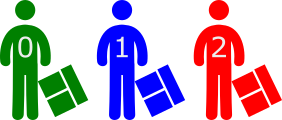
\includegraphics{06MPI/figures/many.png}
  \end{figure}
\item
  each process is independent
\item
  processes can send messages to one another
\end{itemize}

\subsection{MPI in practice}\label{mpi-in-practice}

\subsubsection{Specification and
implementation}\label{specification-and-implementation}

\begin{itemize}
\itemsep1pt\parskip0pt\parsep0pt
\item
  in practice, we use MPI, the
  \href{http://en.wikipedia.org/wiki/Message_Passing_Interface}{Message
  Passing Interface}
\item
  MPI is a \emph{specification} for a \emph{library}
\item
  It is implemented by separate vendors/open-source projects

  \begin{itemize}
  \itemsep1pt\parskip0pt\parsep0pt
  \item
    \href{http://www.open-mpi.org/}{OpenMPI}
  \item
    \href{http://www.mpich.org/}{mpich}
  \end{itemize}
\item
  It is a C library with many many bindings:

  \begin{itemize}
  \itemsep1pt\parskip0pt\parsep0pt
  \item
    Fortran (part of official MPI specification)
  \item
    Python:
    \href{http://www.boost.org/doc/libs/1_55_0/doc/html/mpi/python.html}{boost},
    \href{http://mpi4py.scipy.org/}{mpi4py}
  \item
    R:
    \href{http://cran.r-project.org/web/packages/Rmpi/index.html}{Rmpi}
  \item
    c++:
    \href{http://www.boost.org/doc/libs/1_57_0/doc/html/mpi.html}{boost}
  \end{itemize}
\end{itemize}

\subsubsection{Programming and running}\label{programming-and-running}

\begin{itemize}
\item
  an MPI program is executed with
  \texttt{mpiexec -n N {[}options{]} nameOfProgram {[}args{]}}
\item
  MPI programs call methods from the mpi library
\end{itemize}

\begin{Shaded}
\begin{Highlighting}[]
\DataTypeTok{int} \NormalTok{MPI_Bcast(}\DataTypeTok{void} \NormalTok{*buffer, }\DataTypeTok{int} \NormalTok{count, MPI_Datatype datatype, }\DataTypeTok{int} \NormalTok{root,}
               \NormalTok{MPI_Comm comm)}
\end{Highlighting}
\end{Shaded}

\begin{itemize}
\itemsep1pt\parskip0pt\parsep0pt
\item
  vendors provide wrappers (mpiCC, mpic++) around compilers. Wrappers
  point to header file location and link to right libraries. MPI program
  can be (easily) compiled by substituting
  \texttt{(g++\textbar{}icc) -\textgreater{} mpiCC}
\end{itemize}

\subsubsection{Hello, world!: hello.cc}\label{hello-world-hello.cc}

\begin{Shaded}
\begin{Highlighting}[]
\OtherTok{#include <mpi.h>}
\OtherTok{#include <iostream>}

\DataTypeTok{int} \NormalTok{main(}\DataTypeTok{int} \NormalTok{argc, }\DataTypeTok{char} \NormalTok{* argv[]) \{}
    \CommentTok{/// Must be first call}
    \NormalTok{MPI_Init (&argc, &argv);}
    \CommentTok{/// Now MPI calls possible}

    \CommentTok{/// Size of communicator and process rank}
    \DataTypeTok{int} \NormalTok{rank, size;}
    \NormalTok{MPI_Comm_rank (MPI_COMM_WORLD, &rank);}
    \NormalTok{MPI_Comm_size (MPI_COMM_WORLD, &size);}

    \NormalTok{std::cout << }\StringTok{"Processor "} \NormalTok{<< rank << }\StringTok{" of "} \NormalTok{<< size << }\StringTok{" says hello}\CharTok{\textbackslash{}n}\StringTok{"}\NormalTok{;}

    \CommentTok{/// Must be last MPI call}
    \NormalTok{MPI_Finalize();}
    \CommentTok{/// No more MPI calls from here}
    \KeywordTok{return} \DecValTok{0}\NormalTok{;}
\NormalTok{\}}
\end{Highlighting}
\end{Shaded}

\subsubsection{Hello, world!:
CMakeLists.txt}\label{hello-world-cmakelists.txt}

\begin{Shaded}
\begin{Highlighting}[]
\KeywordTok{find_package}\NormalTok{(MPI }\OtherTok{REQUIRED}\NormalTok{)}

\KeywordTok{add_executable}\NormalTok{(hello hello.cc)}
\KeywordTok{target_include_directories}\NormalTok{(hello }\OtherTok{SYSTEM} \OtherTok{PUBLIC} \DecValTok{$\{MPI_INCLUDE_DIRS\}}\NormalTok{)}
\KeywordTok{target_link_libraries}\NormalTok{(hello }\OtherTok{PUBLIC} \DecValTok{$\{MPI_LIBRARIES\}}\NormalTok{)}
\end{Highlighting}
\end{Shaded}

\subsubsection{Hello, world!: compiling and
running}\label{hello-world-compiling-and-running}

On aristotle.rc.ucl.ac.uk:

\begin{itemize}
\itemsep1pt\parskip0pt\parsep0pt
\item
  load modules: \texttt{module load GCC/4.7.2 OpenMPI/1.6.4-GCC-4.7.2}
  \texttt{module load cmake/2.8.10.2}
\item
  create files ``hello.cc'' and ``CMakeLists.txt'' in some directory
\item
  create build directory \texttt{mkdir build \&\& cd build}
\item
  run cmake and make \texttt{cmake .. \&\& make}
\item
  run the code \texttt{mpiexec -n 4 hello}
\end{itemize}

\subsubsection{Hello, world! dissected}\label{hello-world-dissected}

\begin{itemize}
\item
  MPI calls \emph{must} appear beween \texttt{MPI\_Init} and
  \texttt{MPI\_Finalize}
\item
  Groups of processes are handled by a communicator.
  \texttt{MPI\_COMM\_WORLD} handles the group of all processes.
  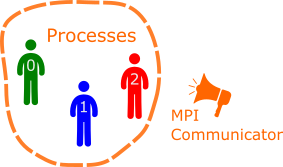
\includegraphics{06MPI/figures/world.png}
\item
  Size of group and rank (order) of process in group
\item
  By \emph{convention}, process of rank 0 is \emph{special} and called
  \emph{root}
\end{itemize}

\subsubsection{MPI with CATCH}\label{mpi-with-catch}

Running MPI unit-tests requires \texttt{MPI\_Init} and
\texttt{MPI\_Finalize} before and after the test framework (\emph{not}
inside the tests).

\begin{Shaded}
\begin{Highlighting}[]

\OtherTok{#include <mpi.h>}
\CommentTok{// Next line tells CATCH we will use our own main function}
\OtherTok{#define CATCH_CONFIG_RUNNER}
\OtherTok{#include "catch.hpp"}

\NormalTok{TEST_CASE(}\StringTok{"Just test I exist"}\NormalTok{) \{}
    \DataTypeTok{int} \NormalTok{rank, size;}
    \NormalTok{MPI_Comm_rank (MPI_COMM_WORLD, &rank);}
    \NormalTok{MPI_Comm_size (MPI_COMM_WORLD, &size);}
    \NormalTok{CHECK(size > }\DecValTok{0}\NormalTok{); CHECK(rank >= }\DecValTok{0}\NormalTok{);}
\NormalTok{\}}

\DataTypeTok{int} \NormalTok{main(}\DataTypeTok{int} \NormalTok{argc, }\DataTypeTok{char} \NormalTok{* argv[]) \{}
    \NormalTok{MPI_Init (&argc, &argv);}
    \DataTypeTok{int} \NormalTok{result = Catch::Session().run(argc, argv);}
    \NormalTok{MPI_Finalize();}
    \KeywordTok{return} \NormalTok{result;}
\NormalTok{\}}
\end{Highlighting}
\end{Shaded}

\subsection{Point to point
communication}\label{point-to-point-communication}

\subsubsection{Many point-2-point communication
schemes}\label{many-point-2-point-communication-schemes}

Can you think of two behaviours for message passing?

\begin{figure}[htbp]
\centering
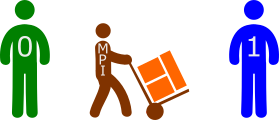
\includegraphics{06MPI/figures/mpi.png}
\end{figure}

\begin{itemize}
\itemsep1pt\parskip0pt\parsep0pt
\item
  Process 0 can (i) give message and then either (ii) leave or (iii)
  wait for acknowledgements
\item
  Process 1 can (i) receive message
\item
  MPI can (i) receive message, (ii) deliver message, (iii) deliver
  acknowledgments
\end{itemize}

\subsubsection{Blocking synchronous
send}\label{blocking-synchronous-send}

\begin{longtable}[c]{@{}ll@{}}
\toprule\addlinespace
Stage & Figure
\\\addlinespace
\midrule\endhead
a. 0, 1, and MPI stand ready: &

\includegraphics{06MPI/figures/sync0.png}
\\\addlinespace
b. message dropped off by 0: & 
\includegraphics{06MPI/figures/sync1.png}
\\\addlinespace
c. transit: & 
\includegraphics{06MPI/figures/syncT.png}
\\\addlinespace
d. message received by 1 & 
\includegraphics{06MPI/figures/syncA.png}
\\\addlinespace
e. receipt received by 0 & 
\includegraphics{06MPI/figures/syncR.png}
\\\addlinespace
\bottomrule
\end{longtable}

\subsubsection{Blocking send}\label{blocking-send}

\begin{longtable}[c]{@{}ll@{}}
\toprule\addlinespace
Stage & Figure
\\\addlinespace
\midrule\endhead
a. 0, 1, and MPI stand ready: &

\includegraphics{06MPI/figures/sync0.png}
\\\addlinespace
b. message dropped off by 0: & 
\includegraphics{06MPI/figures/sync1.png}
\\\addlinespace
c. transit, 0 leaves & 
\includegraphics{06MPI/figures/ssyncT.png}
\\\addlinespace
d. message received by 1 & 
\includegraphics{06MPI/figures/ssyncA.png}
\\\addlinespace
\bottomrule
\end{longtable}

\subsubsection{Non-blocking send}\label{non-blocking-send}

\begin{longtable}[c]{@{}ll@{}}
\toprule\addlinespace
Stage & Figure
\\\addlinespace
\midrule\endhead
a. 0, 1, and MPI stand ready: &

\includegraphics{06MPI/figures/async0.png}
\\\addlinespace
b. 0 leaves message in safebox &

\includegraphics{06MPI/figures/async1.png}
\\\addlinespace
c. transit & 
\includegraphics{06MPI/figures/asyncT.png}
\\\addlinespace
d. message received by 1 & 
\includegraphics{06MPI/figures/asyncA.png}
\\\addlinespace
e. receipt placed in safebox &

\includegraphics{06MPI/figures/asyncR.png}
\\\addlinespace
\bottomrule
\end{longtable}

\subsubsection{Blocking synchronous
send}\label{blocking-synchronous-send-1}

\begin{Shaded}
\begin{Highlighting}[]
\DataTypeTok{int} \NormalTok{MPI_Ssend(}\DataTypeTok{const} \DataTypeTok{void} \NormalTok{*buf, }\DataTypeTok{int} \NormalTok{count, MPI_Datatype datatype, }\DataTypeTok{int} \NormalTok{dest, }\DataTypeTok{int} \NormalTok{tag,}
              \NormalTok{MPI_Comm comm)}
\end{Highlighting}
\end{Shaded}

\begin{longtable}[c]{@{}ll@{}}
\toprule\addlinespace
Parameter & Meaning
\\\addlinespace
\midrule\endhead
buf & Pointer to buffer. Always \texttt{void} because practical C is not
type safe.
\\\addlinespace
count & Size of the buffer. I.e. length of the message to send, in units
of the specified datatype (not bytes)
\\\addlinespace
datatype & Encodes type of the buffer. \texttt{MPI\_INT} for integers,
\texttt{MPI\_CHAR} for characters. Lots of others.
\\\addlinespace
dest & Rank of the \emph{receiving} process
\\\addlinespace
tag & A tag for message book-keeping
\\\addlinespace
comm & The communicator -- usually just \texttt{MPI\_COMM\_WORLD}
\\\addlinespace
return & An error tag. Equals \texttt{MPI\_SUCCESS} on success.
\\\addlinespace
\bottomrule
\end{longtable}

\subsubsection{Blocking receive}\label{blocking-receive}

\begin{Shaded}
\begin{Highlighting}[]
\DataTypeTok{int} \NormalTok{MPI_Recv(}\DataTypeTok{void} \NormalTok{*buf, }\DataTypeTok{int} \NormalTok{count, MPI_Datatype datatype, }\DataTypeTok{int} \NormalTok{source, }\DataTypeTok{int} \NormalTok{tag,}
             \NormalTok{MPI_Comm comm, MPI_Status *status)}
\end{Highlighting}
\end{Shaded}

Good for both synchronous and asynchonous communication

\begin{longtable}[c]{@{}ll@{}}
\toprule\addlinespace
Parameter & Meaning
\\\addlinespace
\midrule\endhead
buf & Pointer to receiving \emph{pre-allocated} buffer
\\\addlinespace
count & Size of the buffer. I.e. maximum length of the message to
receive. See \texttt{MPI\_Get\_count}
\\\addlinespace
datatype & Informs on the type of the buffer
\\\addlinespace
source & Rank of the \emph{sending} process
\\\addlinespace
tag & A tag for message book-keeping
\\\addlinespace
status & `MPI\_STATUS\_IGNORE\texttt{for now. See}MPI\_Get\_count``.
\\\addlinespace
comm & The communicator
\\\addlinespace
return & Error tag
\\\addlinespace
\bottomrule
\end{longtable}

\subsubsection{Example: Blocking synchronous
example}\label{example-blocking-synchronous-example}

Inside a new section in the test framework:

\begin{Shaded}
\begin{Highlighting}[]

      \NormalTok{std::string }\DataTypeTok{const} \NormalTok{peace = }\StringTok{"I come in peace!"}\NormalTok{;}
      \KeywordTok{if}\NormalTok{(rank == }\DecValTok{0}\NormalTok{) \{}
         \DataTypeTok{int} \DataTypeTok{const} \NormalTok{error = MPI_Ssend(}
           \NormalTok{(}\DataTypeTok{void}\NormalTok{*) peace.c_str(), peace.size() + }\DecValTok{1}\NormalTok{, MPI_CHAR, }\DecValTok{1}\NormalTok{, }\DecValTok{42}\NormalTok{, MPI_COMM_WORLD);}
         \CommentTok{// Here, we guarantee that Rank 1 has received the message.}
         \NormalTok{REQUIRE(error ==  MPI_SUCCESS);}
      \NormalTok{\}}
      \KeywordTok{if}\NormalTok{(rank == }\DecValTok{1}\NormalTok{) \{}
          \DataTypeTok{char} \NormalTok{buffer[}\DecValTok{256}\NormalTok{];}
          \DataTypeTok{int} \DataTypeTok{const} \NormalTok{error = MPI_Recv(}
            \NormalTok{buffer, }\DecValTok{256}\NormalTok{, MPI_CHAR, }\DecValTok{0}\NormalTok{, }\DecValTok{42}\NormalTok{, MPI_COMM_WORLD, MPI_STATUS_IGNORE);}
          \NormalTok{REQUIRE(error ==  MPI_SUCCESS);}
          \NormalTok{CHECK(std::string(buffer) == peace);}
      \NormalTok{\}}
\end{Highlighting}
\end{Shaded}

Common bug: Set both sender and receiver to 0. What happens?

\subsubsection{Example: Do you know your C vs C++
strings?}\label{example-do-you-know-your-c-vs-c-strings}

Why the \texttt{+1}?

\begin{Shaded}
\begin{Highlighting}[]
\DataTypeTok{int} \DataTypeTok{const} \NormalTok{error = MPI_Ssend(}
  \NormalTok{(}\DataTypeTok{void}\NormalTok{*) peace.c_str(), peace.size() + }\DecValTok{1}\NormalTok{, MPI_CHAR, }\DecValTok{1}\NormalTok{, }\DecValTok{42}\NormalTok{, MPI_COMM_WORLD);}
\end{Highlighting}
\end{Shaded}

. . .

Because C and C++ \texttt{char const*} strings are null-terminated to
indicate the string is finished, which adds an extra character. However,
\texttt{std::string} abstracts it away. And so its length does
\emph{not} include the null-termination.

\subsubsection{Example: Causing a
dead-lock}\label{example-causing-a-dead-lock}

Watch out for order of send and receive!

Bad:

\begin{Shaded}
\begin{Highlighting}[]
\KeywordTok{if}\NormalTok{(rank == }\DecValTok{0}\NormalTok{) \{}
   \NormalTok{MPI_Ssend (sendbuf, count, MPI_INT, }\DecValTok{1}\NormalTok{, tag, comm);}
   \NormalTok{MPI_Recv (recvbuf, count, MPI_INT, }\DecValTok{1}\NormalTok{, tag, comm, &status);}
\NormalTok{\} }\KeywordTok{else} \NormalTok{\{}
   \NormalTok{MPI_Ssend (sendbuf, count, MPI_INT, }\DecValTok{0}\NormalTok{, tag, comm);}
   \NormalTok{MPI_Recv (recvbuf, count, MPI_INT, }\DecValTok{0}\NormalTok{, tag, comm, &status);}
\NormalTok{\}}
\end{Highlighting}
\end{Shaded}

Good:

\begin{verbatim}
if(rank == 0) {
   MPI_Ssend (sendbuf, count, MPI_INT, 1, tag, comm);
   MPI_Recv (recvbuf, count, MPI_INT, 1, tag, comm, &status);
} else {
   MPI_Recv (recvbuf, count, MPI_INT, 0, tag, comm, &status);
   MPI_Ssend (sendbuf, count, MPI_INT, 0, tag, comm);
}
\end{verbatim}

\subsubsection{Send vs SSend}\label{send-vs-ssend}

Why would we use Send instead of SSend?

\begin{Shaded}
\begin{Highlighting}[]

      \NormalTok{std::string peace = }\StringTok{"I come in peace!"}\NormalTok{;}
      \KeywordTok{if}\NormalTok{(rank == }\DecValTok{0}\NormalTok{) \{}
         \DataTypeTok{int} \DataTypeTok{const} \NormalTok{error = MPI_Send(}
           \NormalTok{(}\DataTypeTok{void}\NormalTok{*) peace.c_str(), peace.size() + }\DecValTok{1}\NormalTok{, MPI_CHAR, }\DecValTok{1}\NormalTok{, }\DecValTok{42}\NormalTok{, MPI_COMM_WORLD);}
         \CommentTok{// We do not guarantee that Rank 1 has received the message yet}
         \CommentTok{// But nor do we necessarily know it hasn't.}
         \CommentTok{// But we are definitely allowed to change the string, as MPI promises}
         \CommentTok{// it has been buffered}
         \NormalTok{peace = }\StringTok{"Shoot to kill!"}\NormalTok{; }\CommentTok{// Safe to reuse the send buffer.}
         \NormalTok{REQUIRE(error ==  MPI_SUCCESS);}
      \NormalTok{\}}
      \KeywordTok{if}\NormalTok{(rank == }\DecValTok{1}\NormalTok{) \{}
          \DataTypeTok{char} \NormalTok{buffer[}\DecValTok{256}\NormalTok{];}
          \DataTypeTok{int} \DataTypeTok{const} \NormalTok{error = MPI_Recv(}
            \NormalTok{buffer, }\DecValTok{256}\NormalTok{, MPI_CHAR, }\DecValTok{0}\NormalTok{, }\DecValTok{42}\NormalTok{, MPI_COMM_WORLD, MPI_STATUS_IGNORE);}
          \NormalTok{REQUIRE(error ==  MPI_SUCCESS);}
          \NormalTok{CHECK(std::string(buffer) == peace);}
      \NormalTok{\}}
\end{Highlighting}
\end{Shaded}

Both guarantee the buffer is safe to reuse. Send makes no guarantee as
to whether it returns early or not. But \emph{SSend} forces a
\emph{synchronisation point}: the codes reach the matching places, with
all processes waiting until all reach that point.

It may come out slightly faster to use Send, since having a
\textbf{synchronisation point} when you don't need one can slow things
down: Suppose (A) runs slightly faster, then (B) does; at the end,
they've both been running fully efficiently.

\begin{figure}[htbp]
\centering
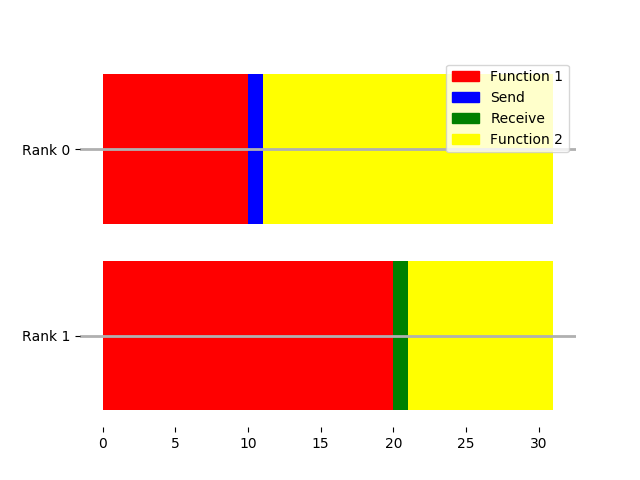
\includegraphics{06MPI/figures/efficient.png}
\end{figure}

Wth a synchronisation point in between, you'll have wasted time:

\begin{figure}[htbp]
\centering
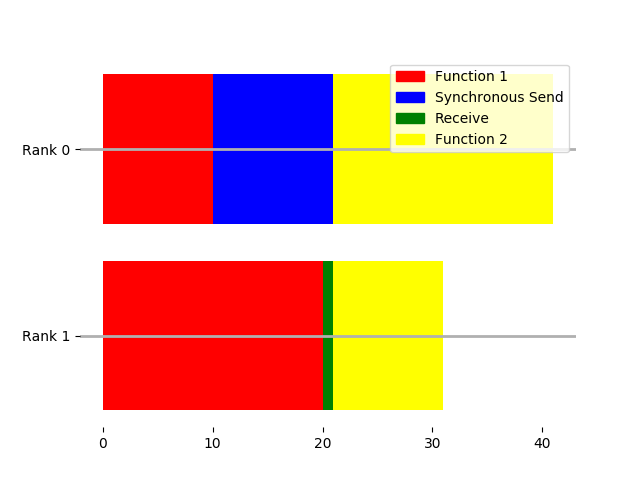
\includegraphics{06MPI/figures/inefficient.png}
\end{figure}

This is only important when there is noise or variability in the
execution time on different processes, but this is often the case.

So unnecessary synchronisation points are bad. The MPI Implementation
may choose to buffer, or synchronise in Send; you're letting MPI guess.

However, if you want to fine tune this to get the best performance, you
should use ISend.

\subsubsection{Non-blocking: ISend/IRecv}\label{non-blocking-isendirecv}

With ISend, we indicate when we want the message to set off.

We receive a handle to the message, of type \texttt{MPI\_Request*} which
we can use to require it has been received, or check.

This produces more complicated code, but you can write code which
\textbf{overlaps calculation with communication}: the message is
travelling, while you get on with something else. We'll see a practical
example of using this next lecture.

\begin{Shaded}
\begin{Highlighting}[]

        \NormalTok{std::string peace = }\StringTok{"I come in peace!"}\NormalTok{;}
        \KeywordTok{if}\NormalTok{(rank == }\DecValTok{0}\NormalTok{) \{}
          \NormalTok{MPI_Request request;}
           \DataTypeTok{int} \NormalTok{error = MPI_Isend(}
             \NormalTok{(}\DataTypeTok{void}\NormalTok{*) peace.c_str(), peace.size() + }\DecValTok{1}\NormalTok{, MPI_CHAR, }\DecValTok{1}\NormalTok{, }\DecValTok{42}\NormalTok{,}
             \NormalTok{MPI_COMM_WORLD, &request);}
           \CommentTok{// We do not guarantee that Rank 1 has received the message yet}
           \CommentTok{// We can carry on, and ANY WORK WE DO NOW WILL OVERLAP WITH THE}
           \CommentTok{// COMMUNICATION}
           \CommentTok{// BUT, we can't safely change the string.}
           \NormalTok{REQUIRE(error ==  MPI_SUCCESS);}
           \CommentTok{// Do some expensive work here}
           \KeywordTok{for} \NormalTok{(}\DataTypeTok{int} \NormalTok{i=}\DecValTok{0}\NormalTok{; i<}\DecValTok{1000}\NormalTok{; i++) \{\}; }\CommentTok{// BUSYNESS FOR EXAMPLE}
           \NormalTok{MPI_Status status;}
           \NormalTok{error = MPI_Wait(&request, &status);}
           \NormalTok{REQUIRE(error ==  MPI_SUCCESS);}
           \CommentTok{// Here, we run code that requires the message to have been}
           \CommentTok{// successfully sent.}
        \NormalTok{\}}
        \KeywordTok{if}\NormalTok{(rank == }\DecValTok{1}\NormalTok{) \{}
            \DataTypeTok{char} \NormalTok{buffer[}\DecValTok{256}\NormalTok{];}
            \DataTypeTok{int} \DataTypeTok{const} \NormalTok{error = MPI_Recv(}
              \NormalTok{buffer, }\DecValTok{256}\NormalTok{, MPI_CHAR, }\DecValTok{0}\NormalTok{, }\DecValTok{42}\NormalTok{, MPI_COMM_WORLD, MPI_STATUS_IGNORE);}
            \NormalTok{REQUIRE(error ==  MPI_SUCCESS);}
            \NormalTok{CHECK(std::string(buffer) == peace);}
        \NormalTok{\}}
\end{Highlighting}
\end{Shaded}

\begin{Shaded}
\begin{Highlighting}[]
\DataTypeTok{int} \NormalTok{MPI_Isend(}\DataTypeTok{const} \DataTypeTok{void} \NormalTok{*buf, }\DataTypeTok{int} \NormalTok{count, MPI_Datatype datatype, }\DataTypeTok{int} \NormalTok{dest, }\DataTypeTok{int} \NormalTok{tag,}
              \NormalTok{MPI_Comm comm, MPI_Request *request)}
\end{Highlighting}
\end{Shaded}

\subsubsection{Pass the parcel:
SendRecv}\label{pass-the-parcel-sendrecv}

Consider a group of N processes in a ring: each has a value, and wants
to ``pass the parcel'' to the left. How would you achieve this with
SSend and Receive?

\begin{Shaded}
\begin{Highlighting}[]

    \DataTypeTok{int} \NormalTok{message = rank*rank;}
    \DataTypeTok{int} \NormalTok{received = -}\DecValTok{7}\NormalTok{;}

    \CommentTok{// Define the ring}
    \DataTypeTok{int} \NormalTok{left = rank}\DecValTok{-1}\NormalTok{;}
    \DataTypeTok{int} \NormalTok{right = rank}\DecValTok{+1}\NormalTok{;}
    \KeywordTok{if} \NormalTok{(rank==}\DecValTok{0}\NormalTok{) \{}
      \NormalTok{left = size}\DecValTok{-1}\NormalTok{;}
    \NormalTok{\}}
    \KeywordTok{if} \NormalTok{(rank == size}\DecValTok{-1}\NormalTok{)\{}
      \NormalTok{right = }\DecValTok{0}\NormalTok{;}
    \NormalTok{\}}
\end{Highlighting}
\end{Shaded}

With synchronous calls each process can only either be sending or
receiving. So the even processes need to send, while the odd ones
receive, then vice-versa. This is clearly inefficient.

\begin{Shaded}
\begin{Highlighting}[]

      \KeywordTok{if} \NormalTok{(rank%}\DecValTok{2} \NormalTok{== }\DecValTok{0}\NormalTok{) \{}
        \DataTypeTok{int} \NormalTok{error = MPI_Ssend(}
          \NormalTok{&message, }\DecValTok{1}\NormalTok{, MPI_INT, left, rank, MPI_COMM_WORLD);}

        \NormalTok{error = MPI_Recv(}
          \NormalTok{&received, }\DecValTok{1}\NormalTok{, MPI_INT, right, right, MPI_COMM_WORLD, MPI_STATUS_IGNORE);}
      \NormalTok{\}}
      \KeywordTok{if} \NormalTok{(rank%}\DecValTok{2} \NormalTok{== }\DecValTok{1}\NormalTok{) \{}

        \DataTypeTok{int} \NormalTok{error = MPI_Recv(}
          \NormalTok{&received, }\DecValTok{1}\NormalTok{, MPI_INT, right, right, MPI_COMM_WORLD, MPI_STATUS_IGNORE);}

        \NormalTok{error = MPI_Ssend(}
          \NormalTok{&message, }\DecValTok{1}\NormalTok{, MPI_INT, left, rank, MPI_COMM_WORLD);}
      \NormalTok{\}}
      \NormalTok{REQUIRE( received == right*right );}
\end{Highlighting}
\end{Shaded}

With ISend/IRecv, this can be achieved in one go: each process posts its
send, then posts its receive, then waits for completion.

\begin{Shaded}
\begin{Highlighting}[]

      \NormalTok{MPI_Request request;}
      \CommentTok{// Everyone sets up their messages to send}
      \DataTypeTok{int} \NormalTok{error = MPI_Isend(}
        \NormalTok{&message, }\DecValTok{1}\NormalTok{, MPI_INT, left, rank, MPI_COMM_WORLD, &request);}

      \CommentTok{// Recv acts as our sync-barrier}
      \NormalTok{error = MPI_Recv(}
        \NormalTok{&received, }\DecValTok{1}\NormalTok{, MPI_INT, right, right, MPI_COMM_WORLD, MPI_STATUS_IGNORE);}

      \CommentTok{// But let's check our send completed:}
      \NormalTok{error = MPI_Wait(&request, MPI_STATUS_IGNORE);}
      \NormalTok{REQUIRE(error ==  MPI_SUCCESS);}

      \NormalTok{REQUIRE( received == right*right );}
\end{Highlighting}
\end{Shaded}

However, this is such a common pattern, that there is a separate MPI
call to make this easier:

\begin{Shaded}
\begin{Highlighting}[]
\DataTypeTok{int} \NormalTok{MPI_Sendrecv(}\DataTypeTok{void} \NormalTok{*sendbuf, }\DataTypeTok{int} \NormalTok{scount, MPI_Datatype stype, }\DataTypeTok{int} \NormalTok{dest, }\DataTypeTok{int} \NormalTok{stag,}
                 \DataTypeTok{void} \NormalTok{*recvbuf, }\DataTypeTok{int} \NormalTok{rcount, MPI_Datatype rtype, }\DataTypeTok{int} \NormalTok{source, }\DataTypeTok{int} \NormalTok{rtag,}
                 \NormalTok{MPI_Comm comm, MPI_Status *status)}
\end{Highlighting}
\end{Shaded}

Each argument is duplicated for the send and receive payloads.

Classroom exercise: implement ring-send using Sendrecv.

\subsubsection{Al(most all) point to
point}\label{almost-all-point-to-point}

Sending messages:

\begin{longtable}[c]{@{}llll@{}}
\toprule\addlinespace
name & Blocking & forces synchronisation point & Buffer-safe
\\\addlinespace
\midrule\endhead
MPI\_Ssend & yes & yes & yes
\\\addlinespace
MPI\_Send & maybe & no & yes
\\\addlinespace
MPI\_Isend & no & no & no
\\\addlinespace
\bottomrule
\end{longtable}

Receiving messages:

\begin{longtable}[c]{@{}ll@{}}
\toprule\addlinespace
name & blocking
\\\addlinespace
\midrule\endhead
MPI\_Recv & yes
\\\addlinespace
MPI\_Irecv & no
\\\addlinespace
\bottomrule
\end{longtable}

\subsection{Collective Communication}\label{collective-communication}

\subsubsection{Many possible communication
schemes}\label{many-possible-communication-schemes}

Think of two possible forms of \emph{collective} communications:

\begin{itemize}
\itemsep1pt\parskip0pt\parsep0pt
\item
  give a beginning state
\item
  give an end state
\end{itemize}

\begin{figure}[htbp]
\centering

\includegraphics{06MPI/figures/collective.png}
\end{figure}

\subsubsection{Broadcast: one to many}\label{broadcast-one-to-many}

\begin{longtable}[c]{@{}ll@{}}
\toprule\addlinespace
State & Figure
\\\addlinespace
\midrule\endhead
data in 0, no data in 1, 2 &

\includegraphics{06MPI/figures/broadcast0.png}
\\\addlinespace
data from 0 sent to 0, 1 &

\includegraphics{06MPI/figures/broadcast1.png}
\\\addlinespace
\bottomrule
\end{longtable}

\subsubsection{Gather: many to one}\label{gather-many-to-one}

\begin{longtable}[c]{@{}ll@{}}
\toprule\addlinespace
State & Figure
\\\addlinespace
\midrule\endhead
data in 0, 1, 2 & 
\includegraphics{06MPI/figures/collective.png}
\\\addlinespace
data from 1, 2 sent to 0 & 
\includegraphics{06MPI/figures/gather1.png}
\\\addlinespace
\bottomrule
\end{longtable}

\subsubsection{Scatter: one to many}\label{scatter-one-to-many}

\begin{longtable}[c]{@{}ll@{}}
\toprule\addlinespace
State & Figure
\\\addlinespace
\midrule\endhead
data in 0 & 
\includegraphics{06MPI/figures/gather1.png}
\\\addlinespace
data from 0 in 0, 1, 2 & 
\includegraphics{06MPI/figures/collective.png}
\\\addlinespace
\bottomrule
\end{longtable}

\subsubsection{All to All: many to many}\label{all-to-all-many-to-many}

\begin{longtable}[c]{@{}ll@{}}
\toprule\addlinespace
State & Figure
\\\addlinespace
\midrule\endhead
data in 0, 1, 2 & 
\includegraphics{06MPI/figures/all2all0.png}
\\\addlinespace
from each to each & 
\includegraphics{06MPI/figures/all2all1.png}
\\\addlinespace
\bottomrule
\end{longtable}

\subsubsection{Reduce operation}\label{reduce-operation}

\begin{longtable}[c]{@{}ll@{}}
\toprule\addlinespace
State & Figure
\\\addlinespace
\midrule\endhead
data in 0, 1, 2 & 
\includegraphics{06MPI/figures/collective.png}
\\\addlinespace
Baby Bunny! & 
\includegraphics{06MPI/figures/reduce1.png}
\\\addlinespace
\bottomrule
\end{longtable}

Wherefrom the baby bunny?

. . .

Sum, difference, or any other \emph{binary} operator:

\begin{figure}[htbp]
\centering

\includegraphics{06MPI/figures/BunnyOps.png}
\end{figure}

\subsubsection{Collective operation API}\label{collective-operation-api}

Group synchronisation:

\begin{Shaded}
\begin{Highlighting}[]
\DataTypeTok{int} \NormalTok{MPI_Barrier(MPI_Comm comm);}
\end{Highlighting}
\end{Shaded}

Broadcasting:

\begin{Shaded}
\begin{Highlighting}[]
\DataTypeTok{int} \NormalTok{MPI_Bcast(}\DataTypeTok{void} \NormalTok{*buffer, }\DataTypeTok{int} \NormalTok{count, MPI_Datatype datatype, }\DataTypeTok{int} \NormalTok{root,}
    \NormalTok{MPI_Comm comm)}
\end{Highlighting}
\end{Shaded}

\begin{longtable}[c]{@{}ll@{}}
\toprule\addlinespace
Parameter & Content
\\\addlinespace
\midrule\endhead
buf & Pointer to sending/receiving buffer
\\\addlinespace
count & Size of the buffer/message
\\\addlinespace
datatype & Informs on the type of the buffer
\\\addlinespace
root & Sending processor
\\\addlinespace
comm & The communicator!
\\\addlinespace
return & Error tag
\\\addlinespace
\bottomrule
\end{longtable}

\subsubsection{Example of collective operation
(1)}\label{example-of-collective-operation-1}

Insert into a new CATCH section the following commands

\begin{Shaded}
\begin{Highlighting}[]

      \NormalTok{std::string }\DataTypeTok{const} \NormalTok{peace = }\StringTok{"I come in peace!"}\NormalTok{;}
      \NormalTok{std::string message = }\StringTok{""}\NormalTok{;}
      \DataTypeTok{int} \NormalTok{error;}
      \KeywordTok{if}\NormalTok{(rank == }\DecValTok{0}\NormalTok{) \{}
          \NormalTok{message = peace;}
          \NormalTok{error = MPI_Bcast(}
             \NormalTok{(}\DataTypeTok{void}\NormalTok{*) peace.c_str(), peace.size() + }\DecValTok{1}\NormalTok{, MPI_CHAR, }\DecValTok{0}\NormalTok{, MPI_COMM_WORLD);}
      \NormalTok{\} }\KeywordTok{else} \NormalTok{\{}
          \DataTypeTok{char} \NormalTok{buffer[}\DecValTok{256}\NormalTok{];}
          \NormalTok{error = MPI_Bcast(buffer, }\DecValTok{256}\NormalTok{, MPI_CHAR, }\DecValTok{0}\NormalTok{, MPI_COMM_WORLD);}
          \NormalTok{message = std::string(buffer);}
      \NormalTok{\}}
\end{Highlighting}
\end{Shaded}

\subsubsection{Example of collective operations
(2)}\label{example-of-collective-operations-2}

And then insert the following right after it

\begin{Shaded}
\begin{Highlighting}[]

      \KeywordTok{for}\NormalTok{(}\DataTypeTok{int} \NormalTok{i(}\DecValTok{0}\NormalTok{); i < size; ++i) \{}
          \KeywordTok{if}\NormalTok{(rank == i) \{}
            \NormalTok{INFO(}\StringTok{"Current rank is "} \NormalTok{<< rank);}
            \NormalTok{REQUIRE(error == MPI_SUCCESS);}
            \NormalTok{CHECK(message == peace);}
          \NormalTok{\}}
          \NormalTok{MPI_Barrier(MPI_COMM_WORLD);}
      \NormalTok{\}}
\end{Highlighting}
\end{Shaded}

\subsubsection{Causing deadlocks}\label{causing-deadlocks}

Explain why the following two codes fail.

\begin{enumerate}
\def\labelenumi{\arabic{enumi}.}
\itemsep1pt\parskip0pt\parsep0pt
\item
  Replace the loop in the last fragment with:
\end{enumerate}

\begin{Shaded}
\begin{Highlighting}[]
\KeywordTok{for}\NormalTok{(}\DataTypeTok{int} \NormalTok{i(}\DecValTok{1}\NormalTok{); i < size; ++i) ...}
\end{Highlighting}
\end{Shaded}

\begin{enumerate}
\def\labelenumi{\arabic{enumi}.}
\setcounter{enumi}{1}
\itemsep1pt\parskip0pt\parsep0pt
\item
  Refactor and put everything inside the loop
\end{enumerate}

\begin{Shaded}
\begin{Highlighting}[]
\NormalTok{std::string }\DataTypeTok{const} \NormalTok{peace = }\StringTok{"I come in peace!"}\NormalTok{;}
\NormalTok{std::string message;}
\KeywordTok{for}\NormalTok{(}\DataTypeTok{int} \NormalTok{i(}\DecValTok{0}\NormalTok{); i < size; ++i) \{}
    \KeywordTok{if}\NormalTok{(i == }\DecValTok{0} \KeywordTok{and} \NormalTok{rank == }\DecValTok{0}\NormalTok{) \{ }\CommentTok{/* broadcast */} \NormalTok{\}}
    \KeywordTok{else} \KeywordTok{if}\NormalTok{(rank == i) \{ }\CommentTok{/* broadcast */} \NormalTok{\}}
    \KeywordTok{if}\NormalTok{(rank == i) \{ }\CommentTok{/* testing bit */} \NormalTok{\}}
    \NormalTok{MPI_Barrier(MPI_COMM_WORLD);}
\NormalTok{\}}
\end{Highlighting}
\end{Shaded}

NOTE: a loop with a condition for i == 0 is a common anti-pattern (eg
bad)

\subsubsection{All to all operation}\label{all-to-all-operation}

\begin{Shaded}
\begin{Highlighting}[]
\DataTypeTok{int} \NormalTok{MPI_Scatter(}\DataTypeTok{const} \DataTypeTok{void} \NormalTok{*sendbuf, }\DataTypeTok{int} \NormalTok{sendcount, MPI_Datatype sendtype,}
               \DataTypeTok{void} \NormalTok{*recvbuf, }\DataTypeTok{int} \NormalTok{recvcount, MPI_Datatype recvtype, }\DataTypeTok{int} \NormalTok{root,}
               \NormalTok{MPI_Comm comm)}
\end{Highlighting}
\end{Shaded}

\begin{longtable}[c]{@{}ll@{}}
\toprule\addlinespace
Parameter & Content
\\\addlinespace
\midrule\endhead
sendbuf & Pointer to sending buffer (only significant at root)
\\\addlinespace
sendcount & Size of a \emph{single} message
\\\addlinespace
datatype & Type of the buffer
\\\addlinespace
recvbuf & Pointer to receiving buffers (also at root)
\\\addlinespace
recvcount & Size of the receiving buffer
\\\addlinespace
recvtype & Informs on the type of the receiving buffer
\\\addlinespace
\bottomrule
\end{longtable}

Exercise: Have the root scatter ``This\ldots{}..'' ``message..''
``is.split.'' to 3 processors (including it self).

\subsubsection{Splitting the
communicators}\label{splitting-the-communicators}

Groups of processes can be split according to \emph{color}:

\begin{figure}[htbp]
\centering
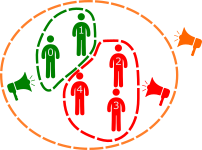
\includegraphics{06MPI/figures/split.png}
\end{figure}

\begin{Shaded}
\begin{Highlighting}[]
\DataTypeTok{int} \NormalTok{MPI_Comm_split(MPI_Comm comm, }\DataTypeTok{int} \NormalTok{color, }\DataTypeTok{int} \NormalTok{key, MPI_Comm *newcomm)}
\end{Highlighting}
\end{Shaded}

\begin{longtable}[c]{@{}ll@{}}
\toprule\addlinespace
Parameter & Content
\\\addlinespace
\midrule\endhead
comm & Communicator that contains all the processes to be split
\\\addlinespace
color & All processes with same color end up in same group
\\\addlinespace
int key & Controls rank in final group
\\\addlinespace
newcomm & Output communicator
\\\addlinespace
\bottomrule
\end{longtable}

\subsubsection{Splitting communicators:
example}\label{splitting-communicators-example}

The following splits processes into two groups with ratio 1:2.

\begin{Shaded}
\begin{Highlighting}[]

    \DataTypeTok{bool} \DataTypeTok{const} \NormalTok{is_apple = rank % }\DecValTok{3} \NormalTok{== }\DecValTok{0}\NormalTok{;}
    \NormalTok{SECTION(}\StringTok{"split 1:3 and keep same process order"}\NormalTok{) \{}
        \NormalTok{MPI_Comm apple_orange;}
        \NormalTok{MPI_Comm_split(MPI_COMM_WORLD, is_apple ? }\DecValTok{0}\NormalTok{: }\DecValTok{1}\NormalTok{, rank, &apple_orange);}

        \DataTypeTok{int} \NormalTok{nrank, nsize;}
        \NormalTok{MPI_Comm_rank(apple_orange, &nrank);}
        \NormalTok{MPI_Comm_size(apple_orange, &nsize);}

        \DataTypeTok{int} \DataTypeTok{const} \NormalTok{div = (size - }\DecValTok{1}\NormalTok{) / }\DecValTok{3}\NormalTok{, napples = }\DecValTok{1} \NormalTok{+ div;}
        \KeywordTok{if}\NormalTok{(is_apple) \{}
           \NormalTok{CHECK(nsize == napples);}
           \NormalTok{CHECK(nrank == rank / }\DecValTok{3}\NormalTok{);}
        \NormalTok{\} }\KeywordTok{else} \NormalTok{\{}
           \NormalTok{CHECK(nsize == size - napples);}
           \NormalTok{CHECK(nrank == rank - }\DecValTok{1} \NormalTok{- (rank / }\DecValTok{3}\NormalTok{));}
        \NormalTok{\}}
    \NormalTok{\}}
\end{Highlighting}
\end{Shaded}

\subsubsection{Splitting communicators:
Exercise}\label{splitting-communicators-exercise}

Exercise:

\begin{itemize}
\itemsep1pt\parskip0pt\parsep0pt
\item
  use ``-rank'' as the key: what happens?
\item
  split into three groups with ratios 1:1:2
\item
  use one of the collective operation on a single group
\end{itemize}

\subsubsection{Scatter operation
solution}\label{scatter-operation-solution}

\begin{Shaded}
\begin{Highlighting}[]

      \NormalTok{std::string }\DataTypeTok{const} \NormalTok{message = }\StringTok{"This message is going to come out in separate channels"}\NormalTok{;}
      \DataTypeTok{int} \NormalTok{N = message.size() / size;}
      \KeywordTok{if}\NormalTok{(message.size() < size) }\KeywordTok{return}\NormalTok{;}

      \DataTypeTok{char} \NormalTok{buffer[}\DecValTok{256}\NormalTok{];}
      \KeywordTok{if}\NormalTok{(rank == }\DecValTok{0}\NormalTok{) \{}
        \DataTypeTok{int} \DataTypeTok{const} \NormalTok{error = MPI_Scatter(}
                \NormalTok{(}\DataTypeTok{void}\NormalTok{*) message.c_str(), N, MPI_CHAR,}
                \NormalTok{buffer, }\DecValTok{256}\NormalTok{, MPI_CHAR, }\DecValTok{0}\NormalTok{, MPI_COMM_WORLD}
        \NormalTok{);}
        \NormalTok{REQUIRE(error == MPI_SUCCESS);}
        \NormalTok{CHECK(message.substr(rank*N, N) == std::string(buffer, N));}
      \NormalTok{\} }\KeywordTok{else} \NormalTok{\{}
        \DataTypeTok{int} \DataTypeTok{const} \NormalTok{error = MPI_Scatter(}
                \NormalTok{NULL, -}\DecValTok{1}\NormalTok{, MPI_CHAR, }\CommentTok{// not significant outside root}
                \NormalTok{buffer, }\DecValTok{256}\NormalTok{, MPI_CHAR, }\DecValTok{0}\NormalTok{, MPI_COMM_WORLD}
        \NormalTok{);}
        \NormalTok{REQUIRE(error == MPI_SUCCESS);}
        \NormalTok{CHECK(message.substr(rank*N, N) == std::string(buffer, N));}
      \NormalTok{\}}
\end{Highlighting}
\end{Shaded}

\subsection{More advanced MPI}\label{more-advanced-mpi}

\subsubsection{Architecture and usage}\label{architecture-and-usage}

\begin{itemize}
\itemsep1pt\parskip0pt\parsep0pt
\item
  depending on library, MPI processes can be \emph{placed} on specific
  node\ldots{}
\item
  \ldots{} and even chained to specific cores
\item
  Fewer processes than core means we can do MPI + openmp:
\item
  some data is distributed (MPI)
\item
  some data is shared (openMP)
\item
  MPI-3 allows for creating/destroying processes dynamically
\end{itemize}

\subsubsection{Splitting communicators}\label{splitting-communicators}

\texttt{MPI\_Group\_*} specify operations to create sets of processes.
In practice, it defines operations on sets:

\begin{itemize}
\itemsep1pt\parskip0pt\parsep0pt
\item
  union
\item
  intersection
\item
  difference
\end{itemize}

And allows the creation of a communicator for the resulting group.

\subsubsection{More MPI data-types}\label{more-mpi-data-types}

It is possible to declare complex data types

\begin{itemize}
\itemsep1pt\parskip0pt\parsep0pt
\item
  strided vectors, e.g.~only one of every element (MPI\_Type\_vector)
\item
  sub-matrices (strided in n axes, n \textgreater{}= 2)
  (MPI\_Type\_Create\_struct)
\item
  irregular strides (MPI\_Type\_indexed)
\end{itemize}

\subsubsection{One sided communication}\label{one-sided-communication}

Prior to MPI-3, both sending and receiving processes must be aware of
the communication.

One-sided communication allow processes to define a buffer that other
processes can access without their explicit knowledge.

\subsubsection{And also}\label{and-also}

\begin{itemize}
\itemsep1pt\parskip0pt\parsep0pt
\item
  Cartesian grid topology where process (1, 1) is neighbor of (0, 1),
  (1, 0), (2, 1), (1, 2). With simplified operations to send data EAST,
  WEST, UP, DOWN\ldots{}.
\item
  More complex graph topologies
\item
  non-blocking collective operations
\end{itemize}

\section{MPI Design Example}\label{mpi-design-example}

\subsection{MPI Design Example}\label{mpi-design-example-1}

\subsubsection{Objectives for this
chapter}\label{objectives-for-this-chapter}

In this chapter, we give an extended introduction to a particular
parallel programming example, introducing some common programming
patterns which occur in working with MPI.

\subsection{Smooth Life}\label{smooth-life}

\subsubsection{Conway's Game of Life}\label{conways-game-of-life}

The Game of Life is a cellular automaton devised by John Conway in 1970.

A cell, on a square grid, is either alive or dead. On the next
iteration:

\begin{itemize}
\itemsep1pt\parskip0pt\parsep0pt
\item
  An alive cell:
\item
  remains alive if it has 2 or 3 alive neighbours out of 8
\item
  dies (of isolation or overcrowding) otherwise
\item
  A dead cell:
\item
  becomes alive if it has exactly 3 alive neighbours
\item
  stays dead otherwise
\end{itemize}

\subsubsection{Conway's Game of Life}\label{conways-game-of-life-1}

This simple set of rules produces beautiful, complex behaviours:

\begin{figure}[htbp]
\centering

\includegraphics{07MPIExample/figures/gun.png}
\caption{``Gospers glider gun'' by Kieff. Licensed under CC BY-SA 3.0
via Wikimedia Commons.}
\end{figure}

\subsubsection{Smooth Life}\label{smooth-life-1}

Smooth Life, proposed by Stephan Rafler, extends this to continuous
variables:

\begin{itemize}
\itemsep1pt\parskip0pt\parsep0pt
\item
  The neighbourhood is an integral over a ring centered on a point.
\item
  The local state is an integral over the disk inside the ring.
\end{itemize}

(The ring has outer radius 3*inner radius, so that the area ratio of 1:8
matches the grid version.)

\subsubsection{Smooth Life}\label{smooth-life-2}

\begin{itemize}
\itemsep1pt\parskip0pt\parsep0pt
\item
  A point has some degree of aliveness.
\item
  Next timestep, a point's aliveness depends on these two integrals
  ($D(r)$ and $R(r)$)
\item
  The new aliveness $S(D(r),R(d))$ is a smoothly varying function such
  that:
\item
  If $D(d)$ is 1, S will be 1 if $d^{(1)} \leq D(r) \leq d^{(2)}$
\item
  If $R(d)$ is 0, S will be 1 if $b^{(1)}\leq R(r) \leq b^{(2)}$
\end{itemize}

A ``Sigmoid'' function is constructed that smoothly blends between these
limits.

\subsubsection{Smooth Life on a
computer}\label{smooth-life-on-a-computer}

We discretise Smooth Life using a grid, so that the integrals become
sums. The aliveness variable becomes a floating point number.

To avoid the hard-edges of a ``ring'' and ``disk'' defined on a grid, we
weight the sum by the fraction of a cell that would fall inside the ring
or disk:

If the distance $d$ from the edge of the ring is within 0.5 units, we
weight the integral by $2d-1$, so that it smoothly various from 1 just
inside to 0 just outside.

\subsubsection{Smooth Life}\label{smooth-life-3}

Smooth Life shows even more interesting behaviour:

\href{https://www.youtube.com/watch?v=KJe9H6qS82I}{SmoothLifeVideo}

\begin{itemize}
\itemsep1pt\parskip0pt\parsep0pt
\item
  Gliders moving any direction
\item
  ``Tension tubes''
\end{itemize}

\subsubsection{Exercise}\label{exercise-1}

We will create the following two functions:

\begin{itemize}
\item
  a function to compute the two integrals $D(r)$ and $R(r)$ as
  $D(x0, y0) = sum_{i, j \in \mathrm{grid}} F(i, j) \mathrm{Disk}(r=||(i - x0, j - y0)||)$
  with $F(i, j)$ the current value at point $(i, j)$
\item
  the main update function:

  loop over all points $(x, y)$ in field:

  \begin{itemize}
  \itemsep1pt\parskip0pt\parsep0pt
  \item
    compute integrals centered at $(x, y)$
  \item
    update the field using the transiontion function
  \end{itemize}
\end{itemize}

All other functions, including the transition function, $\mathrm{Disk}$,
etc are given.

\subsubsection{Square domain into a 1-d
vector}\label{square-domain-into-a-1-d-vector}

We wrap the 2d-grid into a one d vector in \emph{row-major} format:
$F(i, j) <==> F(I)$ with $i = I / Nx$ and $j = I \% Nx$, with $Nx$ the
number of points in direction $x$.

\subsubsection{Distances wrap around a
torus}\label{distances-wrap-around-a-torus}

We use periodic boundary conditions: the field is a torus.

\begin{Shaded}
\begin{Highlighting}[]

\DataTypeTok{int} \NormalTok{Smooth::TorusDistance(}\DataTypeTok{int} \NormalTok{x1, }\DataTypeTok{int} \NormalTok{x2, }\DataTypeTok{int} \NormalTok{size) }\DataTypeTok{const} \NormalTok{\{}
  \DataTypeTok{auto} \DataTypeTok{const} \NormalTok{remainder = std::abs(x1 - x2) % size;}
  \KeywordTok{return} \NormalTok{std::min(remainder, std::abs(remainder - size));}
\NormalTok{\}}
\end{Highlighting}
\end{Shaded}

\subsubsection{Smoothed edge of ring and
disk.}\label{smoothed-edge-of-ring-and-disk.}

$\mathrm{Disk}(r)$:

\begin{Shaded}
\begin{Highlighting}[]

\DataTypeTok{double} \NormalTok{Smooth::Disk(distance radius) }\DataTypeTok{const} \NormalTok{\{}
  \KeywordTok{if}\NormalTok{(radius > inner + smoothing / }\DecValTok{2}\NormalTok{)}
    \KeywordTok{return} \FloatTok{0.0}\NormalTok{;}
  \KeywordTok{if}\NormalTok{(radius < inner - smoothing / }\DecValTok{2}\NormalTok{)}
    \KeywordTok{return} \FloatTok{1.0}\NormalTok{;}
  \KeywordTok{return} \NormalTok{(inner + smoothing / }\DecValTok{2} \NormalTok{- radius) / smoothing;}
\NormalTok{\}}
\end{Highlighting}
\end{Shaded}

\subsubsection{Automated tests for
mathematics}\label{automated-tests-for-mathematics}

\begin{Shaded}
\begin{Highlighting}[]

  \NormalTok{SECTION(}\StringTok{"Sigmoid function is correct"}\NormalTok{) \{}
    \DataTypeTok{double} \NormalTok{e = std::exp(}\FloatTok{1.0}\NormalTok{);}
    \NormalTok{REQUIRE(Smooth::Sigmoid(}\FloatTok{1.0}\NormalTok{, }\FloatTok{1.0}\NormalTok{, }\FloatTok{4.0}\NormalTok{) == }\FloatTok{0.5}\NormalTok{);}
    \NormalTok{REQUIRE(std::abs(Smooth::Sigmoid(}\FloatTok{1.0}\NormalTok{, }\FloatTok{0.0}\NormalTok{, }\FloatTok{4.0}\NormalTok{) - e / (}\DecValTok{1} \NormalTok{+ e)) < }\FloatTok{0.0001}\NormalTok{);}
    \NormalTok{REQUIRE(Smooth::Sigmoid(}\DecValTok{10000}\NormalTok{, }\FloatTok{1.0}\NormalTok{, }\FloatTok{4.0}\NormalTok{) == }\FloatTok{1.0}\NormalTok{);}
    \NormalTok{REQUIRE(std::abs(Smooth::Sigmoid(}\FloatTok{0.0}\NormalTok{, }\FloatTok{1.0}\NormalTok{, }\FloatTok{0.1}\NormalTok{)) < }\FloatTok{0.001}\NormalTok{);}
  \NormalTok{\}}
\end{Highlighting}
\end{Shaded}

\subsubsection{Comments}\label{comments-1}

We can see that this is pretty slow:

If the overall grid is $M$ by $N$, and the range of interaction (3* the
inner radius), is $r$, then each time step takes $MNr^2$ calculations:
if we take all of these proportional as we ``fine grain'' our
discretisation (a square domain, and a constant interaction distance in
absolute units), the problem grows like $N^4$!

So let's parallelize!

\subsection{``Ideal'' Domain
decomposition}\label{ideal-domain-decomposition}

\subsubsection{Domain decomposition}\label{domain-decomposition}

One of the most important problems in designing a parallel code is
``Domain Decomposition'':

\begin{itemize}
\itemsep1pt\parskip0pt\parsep0pt
\item
  How will I divide up the calculation between processes?
\end{itemize}

Design objectives in decomposition are:

\begin{itemize}
\itemsep1pt\parskip0pt\parsep0pt
\item
  Minimise communication
\item
  Optimise load balance (Share out work evenly)
\end{itemize}

\subsubsection{Decomposing Smooth Life}\label{decomposing-smooth-life}

We'll go for a 1-d spatial decomposition for smooth life, dividing the
domain into ``Stripes'' along the x-axis.

If we have an $N$ by $M$ domain, and $p$, processes, each process will
be responsible for $NM/p$ cells, and $NMr^2/p$ calculations.

\subsubsection{Static and dynamic
balance}\label{static-and-dynamic-balance}

This will achieve perfect \textbf{static} load balance: the average work
done by each process is the same. If we were not solving in a
rectangular grid, this would have been harder.

However, since the calculation can (perhaps) be done quicker when the
domain is empty, and our field will vary as time passes, we will not
achieve perfect \textbf{dynamic} load balance.

\subsubsection{Communication in Smooth
Life}\label{communication-in-smooth-life}

Given that each cell needs to know the state of cells within a range
$r=3r_d$, where $r_d$ is the inner radius of the neighbourhood ring, and
$r$ the outer radius, we need to get this information to the
neighbouring sites.

This is \emph{great}: we only need to transfer information to
neighbours, not all the other processes. Such ``local'' communication
results in fast code.

The amount of communication to take place each time step is proportional
to $rMp$, but assuming an appropriate network topology exists, each pair
of neighbours can look after their communication at the same time, so
communication will take time proportional to $rMp/p$=$rM$.

\subsubsection{Strong scaling}\label{strong-scaling}

We therefore expect the time taken for a simulation to vary like:
$Mr(k+Nr/p)$. (Where $k$ is a parameter describing the relative time to
communicate one cell's state compared to the time for calculating one
cell )

Thus, we see that for a FIXED problem size, the benefit of parallelism
will disappear and communication will dominate: this is Amdahl's law
again.

\subsubsection{Weak scaling}\label{weak-scaling}

However, if we consider larger and larger problems, growing $N$ as $p$
grows, then we can stop communication overtaking us. This is a common
outcome: \emph{local} problems provide perfect \emph{weak} scaling
(until network congestion or IO problems dominate).

Any NONLOCAL communication, where the total amount of time for
communication to take place grows as the number of processes does (such
as a gather, which takes $p$, a reduction, like $ln(p)$, or an
all-to-all, like $p^2$, means that perfect weak scaling can't be
achieved.)

\subsubsection{~Exercise: Blocking
Collective}\label{exercise-blocking-collective}

We will parallelize the update and integral functions by having each
process work on a contiguous strip of the whole field.

For simplicity, each process owns a full replica of the field in memory.
This is inneficient since each process owns memory describing a part of
the field it will never use. Improving this is fairly easy, but require
some more bookkeeping. Do try it at home!

Exercise: parallelize using a blocking collective

\subsubsection{~Exercise: Halo update}\label{exercise-halo-update}

Parallelize using a non-blocking collective and layer computation and
calculation:

\begin{enumerate}
\def\labelenumi{\arabic{enumi}.}
\itemsep1pt\parskip0pt\parsep0pt
\item
  send data (part of the field) other processes need
\item
  update part of owned field that does not need data from other
  processes
\item
  receive data from other processes
\item
  update part of owned field that needs data from other proceses
\end{enumerate}

This is called a halo update and quite common to domain decomposition
problems. We can layer communication and computation even more by
splitting over data on the left and on the right boundaries.

\subsubsection{~Header}\label{header-1}

\begin{Shaded}
\begin{Highlighting}[]
\OtherTok{#include <string>}
\OtherTok{#include <vector>}
\OtherTok{#include <mpi.h>}

\KeywordTok{typedef} \DataTypeTok{double} \NormalTok{density;}
\KeywordTok{typedef} \DataTypeTok{double} \NormalTok{distance;}
\KeywordTok{typedef} \DataTypeTok{double} \NormalTok{filling;}

\KeywordTok{class} \NormalTok{Smooth \{}
\KeywordTok{public}\NormalTok{:}
  \NormalTok{Smooth(}\DataTypeTok{int} \NormalTok{sizex = }\DecValTok{100}\NormalTok{, }\DataTypeTok{int} \NormalTok{sizey = }\DecValTok{100}\NormalTok{, distance inner = }\FloatTok{21.0}\NormalTok{, filling birth_1 = }\FloatTok{0.278}\NormalTok{,}
         \NormalTok{filling birth_2 = }\FloatTok{0.365}\NormalTok{, filling death_1 = }\FloatTok{0.267}\NormalTok{, filling death_2 = }\FloatTok{0.445}\NormalTok{,}
         \NormalTok{filling smoothing_disk = }\FloatTok{0.147}\NormalTok{, filling smoothing_ring = }\FloatTok{0.028}\NormalTok{);}
  \DataTypeTok{int} \NormalTok{Size() }\DataTypeTok{const}\NormalTok{;}
  \DataTypeTok{int} \NormalTok{Sizex() }\DataTypeTok{const}\NormalTok{;}
  \DataTypeTok{int} \NormalTok{Sizey() }\DataTypeTok{const}\NormalTok{;}
  \DataTypeTok{int} \NormalTok{Range() }\DataTypeTok{const}\NormalTok{;}
  \DataTypeTok{int} \NormalTok{Frame() }\DataTypeTok{const}\NormalTok{;}
  \DataTypeTok{const} \NormalTok{std::vector<density> &Field() }\DataTypeTok{const}\NormalTok{;}
  \DataTypeTok{void} \NormalTok{Field(std::vector<density> }\DataTypeTok{const} \NormalTok{&input);}

  \CommentTok{//! }\KeywordTok{\textbackslash{}brief}\CommentTok{ Piecewise linear function defining the disk}
  \CommentTok{//! }\KeywordTok{\textbackslash{}details}
  \CommentTok{//! - 1 inside the disk}
  \CommentTok{//! - 0 outside the disk}
  \CommentTok{//! - 0 < x < 1 in the smoothing region}
  \DataTypeTok{double} \NormalTok{Disk(distance radius) }\DataTypeTok{const}\NormalTok{;}
  \CommentTok{//! }\KeywordTok{\textbackslash{}brief}\CommentTok{ Piecewise linear function defining the ring}
  \CommentTok{//! }\KeywordTok{\textbackslash{}details}
  \CommentTok{//! - 1 inside the ring}
  \CommentTok{//! - 0 outside the ring}
  \CommentTok{//! - 0 < x < 1 in the smoothing region}
  \DataTypeTok{double} \NormalTok{Ring(distance radius) }\DataTypeTok{const}\NormalTok{;}
  \CommentTok{//! Smooth step function: 0 at -infty, 1 at +infty}
  \DataTypeTok{static} \DataTypeTok{double} \NormalTok{Sigmoid(}\DataTypeTok{double} \NormalTok{variable, }\DataTypeTok{double} \NormalTok{center, }\DataTypeTok{double} \NormalTok{width);}
  \CommentTok{//! $e^\{-4x / width\}$: 0 at -infty, 1 at +infty}
  \DataTypeTok{static} \DataTypeTok{double} \NormalTok{Sigmoid(}\DataTypeTok{double} \NormalTok{x, }\DataTypeTok{double} \NormalTok{width);}
  \NormalTok{density Transition(filling disk, filling ring) }\DataTypeTok{const}\NormalTok{;}
  \DataTypeTok{int} \NormalTok{TorusDistance(}\DataTypeTok{int} \NormalTok{x1, }\DataTypeTok{int} \NormalTok{x2, }\DataTypeTok{int} \NormalTok{size) }\DataTypeTok{const}\NormalTok{;}
  \DataTypeTok{double} \NormalTok{Radius(}\DataTypeTok{int} \NormalTok{x1, }\DataTypeTok{int} \NormalTok{y1, }\DataTypeTok{int} \NormalTok{x2, }\DataTypeTok{int} \NormalTok{y2) }\DataTypeTok{const}\NormalTok{;}
  \CommentTok{// Value of the integral over a single ring}
  \DataTypeTok{double} \NormalTok{NormalisationRing() }\DataTypeTok{const}\NormalTok{;}
  \CommentTok{// Value of the integral over a single disk}
  \DataTypeTok{double} \NormalTok{NormalisationDisk() }\DataTypeTok{const}\NormalTok{;}
  \CommentTok{//! Sets the playing field to random values}
  \DataTypeTok{void} \NormalTok{SeedRandom();}
  \CommentTok{//! Sets the playing field to constant values}
  \DataTypeTok{void} \NormalTok{SeedConstant(density constant = }\DecValTok{0}\NormalTok{);}
  \CommentTok{//! Adds a disk to the playing field}
  \DataTypeTok{void} \NormalTok{AddDisk(}\DataTypeTok{int} \NormalTok{x0 = }\DecValTok{0}\NormalTok{, }\DataTypeTok{int} \NormalTok{y0 = }\DecValTok{0}\NormalTok{);}
  \CommentTok{//! Adds a ring to the playing field}
  \DataTypeTok{void} \NormalTok{AddRing(}\DataTypeTok{int} \NormalTok{x0 = }\DecValTok{0}\NormalTok{, }\DataTypeTok{int} \NormalTok{y0 = }\DecValTok{0}\NormalTok{);}
  \CommentTok{//! Sets a single pixel in the field}
  \DataTypeTok{void} \NormalTok{AddPixel(}\DataTypeTok{int} \NormalTok{x0, }\DataTypeTok{int} \NormalTok{y0, density value);}
  \CommentTok{//! Moves to next step}
  \DataTypeTok{void} \NormalTok{Update();}
  \CommentTok{//! Prints current field to standard output}
  \DataTypeTok{void} \NormalTok{Write(std::ostream &out);}

  \CommentTok{//! Returns \{disk, ring\} integrals at point (x, y)}
  \NormalTok{std::pair<density, density> Integrals(}\DataTypeTok{int} \NormalTok{x, }\DataTypeTok{int} \NormalTok{y) }\DataTypeTok{const}\NormalTok{;}

  \CommentTok{//! Linear index from cartesian index}
  \DataTypeTok{int} \NormalTok{Index(}\DataTypeTok{int} \NormalTok{i, }\DataTypeTok{int} \NormalTok{j) }\DataTypeTok{const}\NormalTok{;}
  \CommentTok{//! Cartesian index from linear index}
  \NormalTok{std::pair<}\DataTypeTok{int}\NormalTok{, }\DataTypeTok{int}\NormalTok{> Index(}\DataTypeTok{int} \NormalTok{i) }\DataTypeTok{const}\NormalTok{;}

\KeywordTok{private}\NormalTok{:}
  \DataTypeTok{int} \NormalTok{sizex, sizey;}
  \NormalTok{std::vector<density> field, work_field;}
  \NormalTok{filling birth_1, death_1;}
  \NormalTok{filling birth_2, death_2;}
  \NormalTok{filling smoothing_disk, smoothing_ring;}
  \NormalTok{distance inner, outer, smoothing;}
  \DataTypeTok{int} \NormalTok{frame;}
  \DataTypeTok{double} \NormalTok{normalisation_disk, normalisation_ring;}

\OtherTok{#ifdef HAS_MPI}
\KeywordTok{public}\NormalTok{:}
  \NormalTok{MPI_Comm }\DataTypeTok{const} \NormalTok{&Communicator() }\DataTypeTok{const} \NormalTok{\{ }\KeywordTok{return} \NormalTok{communicator; \}}
  \DataTypeTok{void} \NormalTok{Communicator(MPI_Comm }\DataTypeTok{const} \NormalTok{&comm) \{ communicator = comm; \}}

  \CommentTok{//! Update which layers computation and communication}
  \DataTypeTok{void} \NormalTok{LayeredUpdate();}

  \CommentTok{//! Figure start owned sites for given rank}
  \DataTypeTok{static} \DataTypeTok{int} \NormalTok{OwnedStart(}\DataTypeTok{int} \NormalTok{nsites, }\DataTypeTok{int} \NormalTok{ncomms, }\DataTypeTok{int} \NormalTok{rank);}

  \CommentTok{//! }\KeywordTok{\textbackslash{}brief}\CommentTok{ Syncs fields between processes}
  \CommentTok{//! }\KeywordTok{\textbackslash{}details}\CommentTok{ Assumes that each rank owns the sites given by OwnedRange.}
  \DataTypeTok{static} \DataTypeTok{void} \NormalTok{WholeFieldBlockingSync(std::vector<density> &field, MPI_Comm }\DataTypeTok{const} \NormalTok{&comm);}

  \CommentTok{//! }\KeywordTok{\textbackslash{}brief}\CommentTok{ Syncs fields between processes without blocking}
  \CommentTok{//! }\KeywordTok{\textbackslash{}details}\CommentTok{ Assumes that each rank owns the sites given by OwnedRange.}
  \DataTypeTok{static} \NormalTok{MPI_Request WholeFieldNonBlockingSync(std::vector<density> &field, MPI_Comm }\DataTypeTok{const} \NormalTok{&comm);}
\KeywordTok{private}\NormalTok{:}
  \NormalTok{MPI_Comm communicator;}
\OtherTok{#endif}
\NormalTok{\};}
\end{Highlighting}
\end{Shaded}

\subsubsection{~Tests}\label{tests-1}

\begin{Shaded}
\begin{Highlighting}[]
\OtherTok{#ifndef HAS_MPI}
\OtherTok{#define CATCH_CONFIG_MAIN}
\OtherTok{#else}
\OtherTok{#define CATCH_CONFIG_RUNNER}
\OtherTok{#include <catch.hpp>}
\OtherTok{#endif}

\OtherTok{#include <cmath>}
\OtherTok{#include <random>}
\OtherTok{#include "catch.hpp"}
\OtherTok{#include "smooth.h"}

\NormalTok{TEST_CASE(}\StringTok{"Compute Integrals"}\NormalTok{) \{}
  \NormalTok{Smooth smooth(}\DecValTok{300}\NormalTok{, }\DecValTok{300}\NormalTok{);}
  \NormalTok{smooth.SeedConstant(}\DecValTok{0}\NormalTok{);}

  \CommentTok{// check for different positions in the torus}
  \KeywordTok{for}\NormalTok{(}\DataTypeTok{auto} \DataTypeTok{const} \NormalTok{x : \{}\DecValTok{150}\NormalTok{, }\DecValTok{298}\NormalTok{, }\DecValTok{0}\NormalTok{\})}
    \KeywordTok{for}\NormalTok{(}\DataTypeTok{auto} \DataTypeTok{const} \NormalTok{y : \{}\DecValTok{150}\NormalTok{, }\DecValTok{298}\NormalTok{, }\DecValTok{0}\NormalTok{\}) \{}
      \NormalTok{SECTION(}\StringTok{"At position ("} \NormalTok{+ std::to_string(x) + }\StringTok{", "} \NormalTok{+ std::to_string(y) + }\StringTok{")"}\NormalTok{) \{}
        \NormalTok{SECTION(}\StringTok{"Ring only"}\NormalTok{) \{}
          \NormalTok{smooth.AddRing(}\DecValTok{150}\NormalTok{, }\DecValTok{150}\NormalTok{);}

          \DataTypeTok{auto} \DataTypeTok{const} \NormalTok{result = smooth.Integrals(}\DecValTok{150}\NormalTok{, }\DecValTok{150}\NormalTok{);}
          \CommentTok{// 0.1 accuracy because of smoothing}
          \NormalTok{CHECK(std::get<}\DecValTok{0}\NormalTok{>(result) == Approx(}\DecValTok{0}\NormalTok{).epsilon(}\FloatTok{0.1}\NormalTok{));}
          \NormalTok{CHECK(std::get<}\DecValTok{1}\NormalTok{>(result) == Approx(}\DecValTok{1}\NormalTok{).epsilon(}\FloatTok{0.1}\NormalTok{));}
        \NormalTok{\}}

        \NormalTok{SECTION(}\StringTok{"Disk only"}\NormalTok{) \{}
          \NormalTok{smooth.AddDisk(}\DecValTok{150}\NormalTok{, }\DecValTok{150}\NormalTok{);}
          \DataTypeTok{auto} \DataTypeTok{const} \NormalTok{result = smooth.Integrals(}\DecValTok{150}\NormalTok{, }\DecValTok{150}\NormalTok{);}
          \NormalTok{CHECK(std::get<}\DecValTok{0}\NormalTok{>(result) == Approx(}\DecValTok{1}\NormalTok{).epsilon(}\FloatTok{0.1}\NormalTok{));}
          \NormalTok{CHECK(std::get<}\DecValTok{1}\NormalTok{>(result) == Approx(}\DecValTok{0}\NormalTok{).epsilon(}\FloatTok{0.1}\NormalTok{));}
        \NormalTok{\}}

        \NormalTok{SECTION(}\StringTok{"Disk and ring"}\NormalTok{) \{}
          \NormalTok{smooth.AddRing(}\DecValTok{150}\NormalTok{, }\DecValTok{150}\NormalTok{);}
          \NormalTok{smooth.AddDisk(}\DecValTok{150}\NormalTok{, }\DecValTok{150}\NormalTok{);}
          \DataTypeTok{auto} \DataTypeTok{const} \NormalTok{result = smooth.Integrals(}\DecValTok{150}\NormalTok{, }\DecValTok{150}\NormalTok{);}
          \NormalTok{CHECK(std::get<}\DecValTok{0}\NormalTok{>(result) == Approx(}\DecValTok{1}\NormalTok{).epsilon(}\FloatTok{0.1}\NormalTok{));}
          \NormalTok{CHECK(std::get<}\DecValTok{1}\NormalTok{>(result) == Approx(}\DecValTok{1}\NormalTok{).epsilon(}\FloatTok{0.1}\NormalTok{));}
        \NormalTok{\}}
      \NormalTok{\}}
    \NormalTok{\}}
\NormalTok{\}}

\NormalTok{TEST_CASE(}\StringTok{"Update"}\NormalTok{) \{}
  \CommentTok{// just test playing with a single pixel lit up sufficiently that the}
  \CommentTok{// transition is non-zero in the ring.}
  \DataTypeTok{auto} \DataTypeTok{const} \NormalTok{radius = }\DecValTok{5}\NormalTok{;}
  \NormalTok{Smooth smooth(}\DecValTok{100}\NormalTok{, }\DecValTok{100}\NormalTok{, radius);}
  \NormalTok{smooth.AddPixel(}\DecValTok{50}\NormalTok{, }\DecValTok{50}\NormalTok{, }\FloatTok{0.3} \NormalTok{* smooth.NormalisationRing());}
  \NormalTok{CHECK(std::get<}\DecValTok{0}\NormalTok{>(smooth.Integrals(}\DecValTok{50}\NormalTok{, }\DecValTok{50}\NormalTok{))}
        \NormalTok{== Approx(}\FloatTok{0.3} \NormalTok{* smooth.NormalisationRing() / smooth.NormalisationDisk()));}

  \CommentTok{// check the integrals are numbers for which Transition gives non-zero result}
  \CommentTok{// in the ring}
  \NormalTok{CHECK(std::get<}\DecValTok{1}\NormalTok{>(smooth.Integrals(}\DecValTok{50}\NormalTok{, }\DecValTok{50}\NormalTok{)) == Approx(}\DecValTok{0}\NormalTok{));}
  \NormalTok{CHECK(std::get<}\DecValTok{0}\NormalTok{>(smooth.Integrals(}\DecValTok{40}\NormalTok{, }\DecValTok{40}\NormalTok{)) == Approx(}\DecValTok{0}\NormalTok{));}
  \NormalTok{CHECK(std::get<}\DecValTok{1}\NormalTok{>(smooth.Integrals(}\DecValTok{40}\NormalTok{, }\DecValTok{40}\NormalTok{)) == Approx(}\FloatTok{0.3}\NormalTok{));}
  \NormalTok{CHECK(std::get<}\DecValTok{0}\NormalTok{>(smooth.Integrals(}\DecValTok{42}\NormalTok{, }\DecValTok{39}\NormalTok{)) == Approx(}\DecValTok{0}\NormalTok{));}
  \NormalTok{CHECK(std::get<}\DecValTok{1}\NormalTok{>(smooth.Integrals(}\DecValTok{42}\NormalTok{, }\DecValTok{39}\NormalTok{)) == Approx(}\FloatTok{0.3}\NormalTok{));}

  \CommentTok{// Now call update}
  \NormalTok{smooth.Update();}
  \DataTypeTok{auto} \DataTypeTok{const} \NormalTok{field = smooth.Field();}
  \CommentTok{// And check death in the disk}
  \NormalTok{CHECK(field[smooth.Index(}\DecValTok{50}\NormalTok{, }\DecValTok{50}\NormalTok{)] == Approx(}\DecValTok{0}\NormalTok{));}
  \NormalTok{CHECK(field[smooth.Index(}\DecValTok{51}\NormalTok{, }\DecValTok{52}\NormalTok{)] == Approx(}\DecValTok{0}\NormalTok{));}
  \CommentTok{// And check life in the ring}
  \NormalTok{CHECK(field[smooth.Index(}\DecValTok{45}\NormalTok{, }\DecValTok{45}\NormalTok{)] == Approx(smooth.Transition(}\DecValTok{0}\NormalTok{, }\FloatTok{0.3}\NormalTok{)));}
  \NormalTok{CHECK(field[smooth.Index(}\DecValTok{42}\NormalTok{, }\DecValTok{39}\NormalTok{)] == Approx(smooth.Transition(}\DecValTok{0}\NormalTok{, }\FloatTok{0.3}\NormalTok{)));}
  \CommentTok{// And check death outside}
  \NormalTok{CHECK(field[smooth.Index(}\DecValTok{15}\NormalTok{, }\DecValTok{15}\NormalTok{)] == Approx(}\DecValTok{0}\NormalTok{));}
\NormalTok{\}}

\OtherTok{#ifdef HAS_MPI}
\NormalTok{TEST_CASE(}\StringTok{"Arithmetics for plitting a field on different nodes"}\NormalTok{) \{}
  \NormalTok{CHECK(Smooth::OwnedStart(}\DecValTok{5}\NormalTok{, }\DecValTok{2}\NormalTok{, }\DecValTok{0}\NormalTok{) == }\DecValTok{0}\NormalTok{);}
  \NormalTok{CHECK(Smooth::OwnedStart(}\DecValTok{5}\NormalTok{, }\DecValTok{2}\NormalTok{, }\DecValTok{1}\NormalTok{) == }\DecValTok{3}\NormalTok{);}

  \KeywordTok{for}\NormalTok{(}\DataTypeTok{int} \NormalTok{i(}\DecValTok{0}\NormalTok{); i < }\DecValTok{5}\NormalTok{; ++i)}
    \NormalTok{CHECK(Smooth::OwnedStart(}\DecValTok{5}\NormalTok{, }\DecValTok{5}\NormalTok{, i) == i);}

  \CommentTok{// with too many procs, some procs have empty ranges}
  \KeywordTok{for}\NormalTok{(}\DataTypeTok{int} \NormalTok{i(}\DecValTok{5}\NormalTok{); i < }\DecValTok{10}\NormalTok{; ++i)}
    \NormalTok{CHECK(Smooth::OwnedStart(}\DecValTok{5}\NormalTok{, }\DecValTok{10}\NormalTok{, i) == }\DecValTok{5}\NormalTok{);}
\NormalTok{\}}

\NormalTok{TEST_CASE(}\StringTok{"Sync whole field"}\NormalTok{) \{}
  \DataTypeTok{int} \NormalTok{rank, ncomms;}
  \NormalTok{MPI_Comm_rank(MPI_COMM_WORLD, &rank);}
  \NormalTok{MPI_Comm_size(MPI_COMM_WORLD, &ncomms);}

  \CommentTok{// Create known field: -1 outside owned range, equal to rank inside}
  \CommentTok{// Different on each process!}
  \CommentTok{// Also, we make sure the size does not split evenly with the number of procs,}
  \CommentTok{// because that is a harder test.}
  \NormalTok{std::vector<density> field(}\DecValTok{5} \NormalTok{* ncomms + ncomms / }\DecValTok{3}\NormalTok{, -}\DecValTok{1}\NormalTok{);}
  \NormalTok{std::fill(field.begin() + Smooth::OwnedStart(field.size(), ncomms, rank),}
            \NormalTok{field.begin() + Smooth::OwnedStart(field.size(), ncomms, rank + }\DecValTok{1}\NormalTok{), rank);}

  \NormalTok{SECTION(}\StringTok{"Blocking synchronisation"}\NormalTok{) \{}
    \NormalTok{Smooth::WholeFieldBlockingSync(field, MPI_COMM_WORLD);}

    \KeywordTok{for}\NormalTok{(}\DataTypeTok{int} \NormalTok{r(}\DecValTok{0}\NormalTok{); r < ncomms; ++r)}
      \NormalTok{CHECK(std::all_of(field.begin() + Smooth::OwnedStart(field.size(), ncomms, r),}
                        \NormalTok{field.begin() + Smooth::OwnedStart(field.size(), ncomms, r + }\DecValTok{1}\NormalTok{),}
                        \NormalTok{[r](density d) \{ }\KeywordTok{return} \NormalTok{std::abs(d - r) < }\FloatTok{1e-8}\NormalTok{; \}));}
  \NormalTok{\}}

  \NormalTok{SECTION(}\StringTok{"Non blocking synchronisation"}\NormalTok{) \{}
    \DataTypeTok{auto} \NormalTok{request = Smooth::WholeFieldNonBlockingSync(field, MPI_COMM_WORLD);}
    \NormalTok{MPI_Wait(&request, MPI_STATUS_IGNORE);}

    \KeywordTok{for}\NormalTok{(}\DataTypeTok{int} \NormalTok{r(}\DecValTok{0}\NormalTok{); r < ncomms; ++r)}
      \NormalTok{CHECK(std::all_of(field.begin() + Smooth::OwnedStart(field.size(), ncomms, r),}
                        \NormalTok{field.begin() + Smooth::OwnedStart(field.size(), ncomms, r + }\DecValTok{1}\NormalTok{),}
                        \NormalTok{[r](density d) \{ }\KeywordTok{return} \NormalTok{std::abs(d - r) < }\FloatTok{1e-8}\NormalTok{; \}));}
  \NormalTok{\}}
\NormalTok{\}}

\NormalTok{TEST_CASE(}\StringTok{"Serial vs parallel"}\NormalTok{) \{}
  \NormalTok{Smooth serial(}\DecValTok{100}\NormalTok{, }\DecValTok{100}\NormalTok{, }\DecValTok{5}\NormalTok{);}
  \NormalTok{Smooth parallel(}\DecValTok{100}\NormalTok{, }\DecValTok{100}\NormalTok{, }\DecValTok{5}\NormalTok{);}
  \NormalTok{parallel.Communicator(MPI_COMM_WORLD);}

  \CommentTok{// generate one field for all Smooth instances}
  \NormalTok{std::vector<density> field(}\DecValTok{100} \NormalTok{* }\DecValTok{100}\NormalTok{);}
  \NormalTok{std::random_device rd; }\CommentTok{// Will be used to obtain a seed for the random number engine}
  \NormalTok{std::mt19937 gen(rd());}
  \NormalTok{std::uniform_real_distribution<> randdist(}\DecValTok{0}\NormalTok{, }\DecValTok{1}\NormalTok{);}
  \NormalTok{std::generate(field.begin(), field.end(), [&randdist, &gen]() \{ }\KeywordTok{return} \NormalTok{randdist(gen); \});}
  \NormalTok{MPI_Bcast(field.data(), field.size(), MPI_DOUBLE, }\DecValTok{0}\NormalTok{, MPI_COMM_WORLD);}

  \CommentTok{// set the fields for both Smooth instances}
  \NormalTok{serial.Field(field);}
  \NormalTok{parallel.Field(field);}

  \DataTypeTok{int} \NormalTok{rank, ncomms;}
  \NormalTok{MPI_Comm_rank(MPI_COMM_WORLD, &rank);}
  \NormalTok{MPI_Comm_size(MPI_COMM_WORLD, &ncomms);}

  \DataTypeTok{auto} \DataTypeTok{const} \NormalTok{start = Smooth::OwnedStart(field.size(), ncomms, rank);}
  \DataTypeTok{auto} \DataTypeTok{const} \NormalTok{end = Smooth::OwnedStart(field.size(), ncomms, rank);}
  \CommentTok{// if this is false, then the test itself is wrong}
  \NormalTok{CHECK(std::equal(serial.Field().begin() + start, serial.Field().begin() + end,}
                   \NormalTok{parallel.Field().begin() + start));}

  \NormalTok{SECTION(}\StringTok{"Blocking synchronization"}\NormalTok{) \{}
    \CommentTok{// check fields are the same in parallel and in serial for a few iterations}
    \KeywordTok{for}\NormalTok{(}\DataTypeTok{int} \NormalTok{i(}\DecValTok{0}\NormalTok{); i < }\DecValTok{3}\NormalTok{; ++i) \{}
      \NormalTok{serial.Update();}
      \NormalTok{parallel.Update();}
      \NormalTok{CHECK(std::equal(serial.Field().begin() + start, serial.Field().begin() + end,}
                       \NormalTok{parallel.Field().begin() + start));}
    \NormalTok{\}}
  \NormalTok{\}}

  \NormalTok{SECTION(}\StringTok{"Layered communication-computation"}\NormalTok{) \{}
    \KeywordTok{for}\NormalTok{(}\DataTypeTok{int} \NormalTok{i(}\DecValTok{0}\NormalTok{); i < }\DecValTok{3}\NormalTok{; ++i) \{}
      \NormalTok{serial.Update();}
      \NormalTok{parallel.LayeredUpdate();}
      \NormalTok{CHECK(std::equal(serial.Field().begin() + start, serial.Field().begin() + end,}
                       \NormalTok{parallel.Field().begin() + start));}
    \NormalTok{\}}
  \NormalTok{\}}
\NormalTok{\}}

\NormalTok{TEST_CASE(}\StringTok{"Smooth model can be instantiated and configured"}\NormalTok{, }\StringTok{"[Smooth]"}\NormalTok{) \{}

  \NormalTok{SECTION(}\StringTok{"Smooth can be constructed"}\NormalTok{) \{}
    \NormalTok{Smooth smooth;}
    \NormalTok{REQUIRE(smooth.Size() == }\DecValTok{10000}\NormalTok{);}
    \NormalTok{REQUIRE(smooth.Field().size() == smooth.Size());}
  \NormalTok{\}}
\NormalTok{\}}

\NormalTok{TEST_CASE(}\StringTok{"Smooth mathematical functions are correct"}\NormalTok{, }\StringTok{"[Smooth]"}\NormalTok{) \{}
  \NormalTok{Smooth smooth;}
  \NormalTok{SECTION(}\StringTok{"Disk support function is correct"}\NormalTok{) \{}
    \NormalTok{REQUIRE(smooth.Disk(}\DecValTok{500}\NormalTok{) == Approx(}\DecValTok{0}\NormalTok{));}
    \NormalTok{REQUIRE(smooth.Disk(}\FloatTok{21.6}\NormalTok{) == }\FloatTok{0.0}\NormalTok{);}
    \NormalTok{REQUIRE(smooth.Disk(}\FloatTok{21.4}\NormalTok{) > }\FloatTok{0.0}\NormalTok{);}
    \NormalTok{REQUIRE(smooth.Disk(}\FloatTok{21.4}\NormalTok{) < }\FloatTok{1.0}\NormalTok{);}
    \NormalTok{REQUIRE(smooth.Disk(}\FloatTok{20.6}\NormalTok{) > }\FloatTok{0.0}\NormalTok{);}
    \NormalTok{REQUIRE(smooth.Disk(}\FloatTok{20.6}\NormalTok{) < }\FloatTok{1.0}\NormalTok{);}
    \NormalTok{REQUIRE(smooth.Disk(}\FloatTok{20.4}\NormalTok{) == Approx(}\FloatTok{1.0}\NormalTok{));}
    \NormalTok{REQUIRE(smooth.Disk(}\FloatTok{19.0}\NormalTok{) == Approx(}\FloatTok{1.0}\NormalTok{));}
    \NormalTok{REQUIRE(smooth.Disk(}\FloatTok{21.0}\NormalTok{) == Approx(}\FloatTok{0.5}\NormalTok{));}
  \NormalTok{\}}
  \NormalTok{SECTION(}\StringTok{"Ring support function is correct"}\NormalTok{) \{}
    \NormalTok{REQUIRE(smooth.Ring(}\DecValTok{22}\NormalTok{) == }\FloatTok{1.0}\NormalTok{);}
    \NormalTok{REQUIRE(smooth.Ring(}\FloatTok{21.6}\NormalTok{) == }\FloatTok{1.0}\NormalTok{);}
    \NormalTok{REQUIRE(smooth.Ring(}\FloatTok{21.4}\NormalTok{) > }\FloatTok{0.0}\NormalTok{);}
    \NormalTok{REQUIRE(smooth.Ring(}\FloatTok{21.4}\NormalTok{) < }\FloatTok{1.0}\NormalTok{);}
    \NormalTok{REQUIRE(smooth.Ring(}\FloatTok{20.6}\NormalTok{) > }\FloatTok{0.0}\NormalTok{);}
    \NormalTok{REQUIRE(smooth.Ring(}\FloatTok{20.6}\NormalTok{) < }\FloatTok{1.0}\NormalTok{);}
    \NormalTok{REQUIRE(smooth.Ring(}\FloatTok{20.4}\NormalTok{) == }\FloatTok{0.0}\NormalTok{);}
    \NormalTok{REQUIRE(smooth.Ring(}\FloatTok{21.0}\NormalTok{) == }\FloatTok{0.5}\NormalTok{);}
    \NormalTok{REQUIRE(smooth.Ring(}\FloatTok{64.0}\NormalTok{) == }\FloatTok{0.0}\NormalTok{);}
    \NormalTok{REQUIRE(smooth.Ring(}\FloatTok{63.6}\NormalTok{) == }\FloatTok{0.0}\NormalTok{);}
    \NormalTok{REQUIRE(smooth.Ring(}\FloatTok{63.4}\NormalTok{) > }\FloatTok{0.0}\NormalTok{);}
    \NormalTok{REQUIRE(smooth.Ring(}\FloatTok{63.4}\NormalTok{) < }\FloatTok{1.0}\NormalTok{);}
    \NormalTok{REQUIRE(smooth.Ring(}\FloatTok{62.6}\NormalTok{) > }\FloatTok{0.0}\NormalTok{);}
    \NormalTok{REQUIRE(smooth.Ring(}\FloatTok{62.6}\NormalTok{) < }\FloatTok{1.0}\NormalTok{);}
    \NormalTok{REQUIRE(smooth.Ring(}\FloatTok{62.4}\NormalTok{) == }\FloatTok{1.0}\NormalTok{);}
    \NormalTok{REQUIRE(smooth.Ring(}\FloatTok{63.0}\NormalTok{) == }\FloatTok{0.5}\NormalTok{);}
  \NormalTok{\}}

  \CommentTok{/// Sigmoid_Test}
  \NormalTok{SECTION(}\StringTok{"Sigmoid function is correct"}\NormalTok{) \{}
    \DataTypeTok{double} \NormalTok{e = std::exp(}\FloatTok{1.0}\NormalTok{);}
    \NormalTok{REQUIRE(Smooth::Sigmoid(}\FloatTok{1.0}\NormalTok{, }\FloatTok{1.0}\NormalTok{, }\FloatTok{4.0}\NormalTok{) == }\FloatTok{0.5}\NormalTok{);}
    \NormalTok{REQUIRE(std::abs(Smooth::Sigmoid(}\FloatTok{1.0}\NormalTok{, }\FloatTok{0.0}\NormalTok{, }\FloatTok{4.0}\NormalTok{) - e / (}\DecValTok{1} \NormalTok{+ e)) < }\FloatTok{0.0001}\NormalTok{);}
    \NormalTok{REQUIRE(Smooth::Sigmoid(}\DecValTok{10000}\NormalTok{, }\FloatTok{1.0}\NormalTok{, }\FloatTok{4.0}\NormalTok{) == }\FloatTok{1.0}\NormalTok{);}
    \NormalTok{REQUIRE(std::abs(Smooth::Sigmoid(}\FloatTok{0.0}\NormalTok{, }\FloatTok{1.0}\NormalTok{, }\FloatTok{0.1}\NormalTok{)) < }\FloatTok{0.001}\NormalTok{);}
  \NormalTok{\}}
  \CommentTok{/// end}
  \NormalTok{SECTION(}\StringTok{"Transition function is correct"}\NormalTok{) \{}
    \NormalTok{REQUIRE(std::abs(smooth.Transition(}\FloatTok{1.0}\NormalTok{, }\FloatTok{0.3}\NormalTok{) - }\FloatTok{1.0}\NormalTok{) < }\FloatTok{0.1}\NormalTok{);}
    \NormalTok{REQUIRE(smooth.Transition(}\FloatTok{1.0}\NormalTok{, }\FloatTok{1.0}\NormalTok{) == Approx(}\DecValTok{0}\NormalTok{));}
    \NormalTok{REQUIRE(std::abs(smooth.Transition(}\FloatTok{0.0}\NormalTok{, }\FloatTok{0.3}\NormalTok{) - }\FloatTok{1.0}\NormalTok{) < }\FloatTok{0.1}\NormalTok{);}
    \NormalTok{REQUIRE(std::abs(smooth.Transition(}\FloatTok{0.0}\NormalTok{, }\FloatTok{0.0}\NormalTok{)) < }\FloatTok{0.1}\NormalTok{);}
  \NormalTok{\}}
  \NormalTok{SECTION(}\StringTok{"Wraparound Distance is correct"}\NormalTok{) \{}
    \NormalTok{REQUIRE(smooth.TorusDistance(}\DecValTok{95}\NormalTok{, }\DecValTok{5}\NormalTok{, }\DecValTok{100}\NormalTok{) == }\DecValTok{10}\NormalTok{);}
    \NormalTok{REQUIRE(smooth.TorusDistance(}\DecValTok{5}\NormalTok{, }\DecValTok{96}\NormalTok{, }\DecValTok{100}\NormalTok{) == }\DecValTok{9}\NormalTok{);}
    \NormalTok{REQUIRE(smooth.TorusDistance(}\DecValTok{5}\NormalTok{, }\DecValTok{10}\NormalTok{, }\DecValTok{100}\NormalTok{) == }\DecValTok{5}\NormalTok{);}
    \NormalTok{REQUIRE(smooth.Radius(}\DecValTok{10}\NormalTok{, }\DecValTok{10}\NormalTok{, }\DecValTok{13}\NormalTok{, }\DecValTok{14}\NormalTok{) == }\FloatTok{5.0}\NormalTok{);}
  \NormalTok{\}}
\NormalTok{\}}

\NormalTok{TEST_CASE(}\StringTok{"NormalisationsAreCorrect"}\NormalTok{) \{}
  \NormalTok{Smooth smooth(}\DecValTok{100}\NormalTok{, }\DecValTok{100}\NormalTok{, }\DecValTok{10}\NormalTok{);}
  \NormalTok{SECTION(}\StringTok{"Disk Normalisation is correct"}\NormalTok{) \{}
    \CommentTok{// Should be roughly pi*radius*radius,}
    \NormalTok{REQUIRE(std::abs(smooth.NormalisationDisk() - }\FloatTok{314.15}\NormalTok{) < }\FloatTok{1.0}\NormalTok{);}
  \NormalTok{\}}
  \NormalTok{SECTION(}\StringTok{"Ring Normalisation is correct"}\NormalTok{) \{}
    \CommentTok{// Should be roughly pi*outer*outer-pi*inner*inner, pi*100*(9-1), 2513.27}
    \NormalTok{REQUIRE(std::abs(smooth.NormalisationRing() - }\FloatTok{2513.27}\NormalTok{) < }\FloatTok{2.0}\NormalTok{);}
  \NormalTok{\}}
\NormalTok{\}}

\NormalTok{TEST_CASE(}\StringTok{"FillingsAreUnityWhenSeeded"}\NormalTok{) \{}
  \NormalTok{Smooth smooth;}
  \NormalTok{smooth.SeedConstant(}\DecValTok{0}\NormalTok{);}
  \NormalTok{SECTION(}\StringTok{"DiskFillingUnityWithDiskSeed"}\NormalTok{) \{}
    \NormalTok{smooth.AddDisk();}
    \NormalTok{REQUIRE(std::get<}\DecValTok{0}\NormalTok{>(smooth.Integrals(}\DecValTok{0}\NormalTok{, }\DecValTok{0}\NormalTok{)) == Approx(}\DecValTok{1}\NormalTok{).epsilon(}\FloatTok{0.1}\NormalTok{));}
  \NormalTok{\}}

  \NormalTok{SECTION(}\StringTok{"Disk Filling Zero With Ring Seed"}\NormalTok{) \{}
    \NormalTok{smooth.AddRing();}
    \NormalTok{REQUIRE(std::get<}\DecValTok{0}\NormalTok{>(smooth.Integrals(}\DecValTok{0}\NormalTok{, }\DecValTok{0}\NormalTok{)) == Approx(}\DecValTok{0}\NormalTok{).epsilon(}\FloatTok{0.1}\NormalTok{));}
  \NormalTok{\}}
  \NormalTok{SECTION(}\StringTok{"RingFillingUnityWithRingSeed"}\NormalTok{) \{}
    \NormalTok{smooth.AddRing();}
    \NormalTok{REQUIRE(std::get<}\DecValTok{1}\NormalTok{>(smooth.Integrals(}\DecValTok{0}\NormalTok{, }\DecValTok{0}\NormalTok{)) == Approx(}\DecValTok{1}\NormalTok{).epsilon(}\FloatTok{0.1}\NormalTok{));}
  \NormalTok{\}}
\NormalTok{\}}

\NormalTok{TEST_CASE(}\StringTok{"FillingFieldHasRangeofValues"}\NormalTok{) \{}
  \NormalTok{Smooth smooth(}\DecValTok{300}\NormalTok{, }\DecValTok{300}\NormalTok{);}
  \NormalTok{smooth.SeedConstant(}\DecValTok{0}\NormalTok{);}
  \NormalTok{smooth.AddRing();}
  \DataTypeTok{double} \NormalTok{min = }\FloatTok{1.0}\NormalTok{;}
  \DataTypeTok{double} \NormalTok{max = }\FloatTok{0.0}\NormalTok{;}
  \KeywordTok{for}\NormalTok{(}\DataTypeTok{int} \NormalTok{x = }\DecValTok{0}\NormalTok{; x < }\DecValTok{300}\NormalTok{; x++) \{}
    \DataTypeTok{double} \NormalTok{filling = std::get<}\DecValTok{1}\NormalTok{>(smooth.Integrals(x, }\DecValTok{0}\NormalTok{));}
    \NormalTok{min = std::min(min, filling);}
    \NormalTok{max = std::max(max, filling);}
  \NormalTok{\}}
  \NormalTok{REQUIRE(min < }\FloatTok{0.2}\NormalTok{);}
  \NormalTok{REQUIRE(max > }\FloatTok{0.4}\NormalTok{);}
\NormalTok{\}}

\DataTypeTok{int} \NormalTok{main(}\DataTypeTok{int} \NormalTok{argc, }\DataTypeTok{const} \DataTypeTok{char} \NormalTok{**argv) \{}
  \CommentTok{// There must be exactly once instance}
  \NormalTok{Catch::Session session;}

  \NormalTok{MPI_Init(&argc, }\KeywordTok{const_cast}\NormalTok{<}\DataTypeTok{char} \NormalTok{***>(&argv));}
  \DataTypeTok{auto} \DataTypeTok{const} \NormalTok{result = session.run();}

  \NormalTok{MPI_Finalize();}

  \KeywordTok{return} \NormalTok{result;}
\NormalTok{\}}
\OtherTok{#endif}
\end{Highlighting}
\end{Shaded}

\subsubsection{~Implementation}\label{implementation-1}

\begin{Shaded}
\begin{Highlighting}[]
\OtherTok{#include <cassert>}
\OtherTok{#include <cmath>}
\OtherTok{#include <cstdlib>}
\OtherTok{#include <iostream>}

\OtherTok{#include "smooth.h"}

\NormalTok{Smooth::Smooth(}\DataTypeTok{int} \NormalTok{sizex, }\DataTypeTok{int} \NormalTok{sizey, distance inner, filling birth_1, filling birth_2,}
               \NormalTok{filling death_1, filling death_2, filling smoothing_disk, filling smoothing_ring)}
    \NormalTok{: sizex(sizex), sizey(sizey), field(sizex * sizey), work_field(sizex * sizey), inner(inner),}
      \NormalTok{birth_1(birth_1), birth_2(birth_2), death_1(death_1), death_2(death_2),}
      \NormalTok{smoothing_disk(smoothing_disk), smoothing_ring(smoothing_ring), outer(inner * }\DecValTok{3}\NormalTok{),}
      \NormalTok{smoothing(}\FloatTok{1.0}\NormalTok{)}
\OtherTok{#ifdef HAS_MPI}
      \NormalTok{,}
      \NormalTok{communicator(MPI_COMM_SELF)}
\OtherTok{#endif}
\NormalTok{\{}
  \NormalTok{normalisation_disk = NormalisationDisk();}
  \NormalTok{normalisation_ring = NormalisationRing();}
\NormalTok{\}}

\DataTypeTok{const} \NormalTok{std::vector<density> &Smooth::Field() }\DataTypeTok{const} \NormalTok{\{ }\KeywordTok{return} \NormalTok{field; \};}
\DataTypeTok{void} \NormalTok{Smooth::Field(std::vector<density> }\DataTypeTok{const} \NormalTok{&input) \{}
  \NormalTok{assert(field.size() == input.size());}
  \NormalTok{field = input;}
\NormalTok{\}}

\DataTypeTok{int} \NormalTok{Smooth::Range() }\DataTypeTok{const} \NormalTok{\{ }\KeywordTok{return} \NormalTok{outer + smoothing / }\DecValTok{2}\NormalTok{; \}}

\DataTypeTok{int} \NormalTok{Smooth::Sizex() }\DataTypeTok{const} \NormalTok{\{ }\KeywordTok{return} \NormalTok{sizex; \}}
\DataTypeTok{int} \NormalTok{Smooth::Sizey() }\DataTypeTok{const} \NormalTok{\{ }\KeywordTok{return} \NormalTok{sizey; \}}
\DataTypeTok{int} \NormalTok{Smooth::Size() }\DataTypeTok{const} \NormalTok{\{ }\KeywordTok{return} \NormalTok{sizex * sizey; \}}

\CommentTok{/// "Disk_Smoothing"}
\DataTypeTok{double} \NormalTok{Smooth::Disk(distance radius) }\DataTypeTok{const} \NormalTok{\{}
  \KeywordTok{if}\NormalTok{(radius > inner + smoothing / }\DecValTok{2}\NormalTok{)}
    \KeywordTok{return} \FloatTok{0.0}\NormalTok{;}
  \KeywordTok{if}\NormalTok{(radius < inner - smoothing / }\DecValTok{2}\NormalTok{)}
    \KeywordTok{return} \FloatTok{1.0}\NormalTok{;}
  \KeywordTok{return} \NormalTok{(inner + smoothing / }\DecValTok{2} \NormalTok{- radius) / smoothing;}
\NormalTok{\}}
\CommentTok{/// end}

\DataTypeTok{double} \NormalTok{Smooth::Ring(distance radius) }\DataTypeTok{const} \NormalTok{\{}
  \KeywordTok{if}\NormalTok{(radius < inner - smoothing / }\DecValTok{2}\NormalTok{)}
    \KeywordTok{return} \FloatTok{0.0}\NormalTok{;}
  \KeywordTok{if}\NormalTok{(radius < inner + smoothing / }\DecValTok{2}\NormalTok{)}
    \KeywordTok{return} \NormalTok{(radius + smoothing / }\DecValTok{2} \NormalTok{- inner) / smoothing;}
  \KeywordTok{if}\NormalTok{(radius < outer - smoothing / }\DecValTok{2}\NormalTok{)}
    \KeywordTok{return} \FloatTok{1.0}\NormalTok{;}
  \KeywordTok{if}\NormalTok{(radius < outer + smoothing / }\DecValTok{2}\NormalTok{)}
    \KeywordTok{return} \NormalTok{(outer + smoothing / }\DecValTok{2} \NormalTok{- radius) / smoothing;}
  \KeywordTok{return} \FloatTok{0.0}\NormalTok{;}
\NormalTok{\}}

\DataTypeTok{double} \NormalTok{Smooth::Sigmoid(}\DataTypeTok{double} \NormalTok{variable, }\DataTypeTok{double} \NormalTok{center, }\DataTypeTok{double} \NormalTok{width) \{}
  \KeywordTok{return} \NormalTok{Sigmoid(variable - center, width);}
\NormalTok{\}}
\DataTypeTok{double} \NormalTok{Smooth::Sigmoid(}\DataTypeTok{double} \NormalTok{x, }\DataTypeTok{double} \NormalTok{width) \{ }\KeywordTok{return} \FloatTok{1.0} \NormalTok{/ (}\FloatTok{1.0} \NormalTok{+ std::exp(-}\FloatTok{4.0} \NormalTok{* x / width)); \}}

\NormalTok{density Smooth::Transition(filling disk, filling ring) }\DataTypeTok{const} \NormalTok{\{}
  \DataTypeTok{auto} \DataTypeTok{const} \NormalTok{sdisk = Sigmoid(disk - }\FloatTok{0.5}\NormalTok{, smoothing_disk);}
  \DataTypeTok{auto} \DataTypeTok{const} \NormalTok{t1 = birth_1 * (}\FloatTok{1.0} \NormalTok{- sdisk) + death_1 * sdisk;}
  \DataTypeTok{auto} \DataTypeTok{const} \NormalTok{t2 = birth_2 * (}\FloatTok{1.0} \NormalTok{- sdisk) + death_2 * sdisk;}
  \KeywordTok{return} \NormalTok{Sigmoid(ring - t1, smoothing_ring) * Sigmoid(t2 - ring, smoothing_ring);}
\NormalTok{\}}

\DataTypeTok{int} \NormalTok{Smooth::Index(}\DataTypeTok{int} \NormalTok{i, }\DataTypeTok{int} \NormalTok{j) }\DataTypeTok{const} \NormalTok{\{ }\KeywordTok{return} \NormalTok{i * Sizex() + j; \}}
\NormalTok{std::pair<}\DataTypeTok{int}\NormalTok{, }\DataTypeTok{int}\NormalTok{> Smooth::Index(}\DataTypeTok{int} \NormalTok{i) }\DataTypeTok{const} \NormalTok{\{ }\KeywordTok{return} \NormalTok{\{i / Sizex(), i % Sizex()\}; \}}

\CommentTok{/// "Torus_Difference"}
\DataTypeTok{int} \NormalTok{Smooth::TorusDistance(}\DataTypeTok{int} \NormalTok{x1, }\DataTypeTok{int} \NormalTok{x2, }\DataTypeTok{int} \NormalTok{size) }\DataTypeTok{const} \NormalTok{\{}
  \DataTypeTok{auto} \DataTypeTok{const} \NormalTok{remainder = std::abs(x1 - x2) % size;}
  \KeywordTok{return} \NormalTok{std::min(remainder, std::abs(remainder - size));}
\NormalTok{\}}
\CommentTok{/// end}

\DataTypeTok{double} \NormalTok{Smooth::Radius(}\DataTypeTok{int} \NormalTok{x1, }\DataTypeTok{int} \NormalTok{y1, }\DataTypeTok{int} \NormalTok{x2, }\DataTypeTok{int} \NormalTok{y2) }\DataTypeTok{const} \NormalTok{\{}
  \DataTypeTok{int} \NormalTok{xdiff = TorusDistance(x1, x2, sizex);}
  \DataTypeTok{int} \NormalTok{ydiff = TorusDistance(y1, y2, sizey);}
  \KeywordTok{return} \NormalTok{std::sqrt(xdiff * xdiff + ydiff * ydiff);}
\NormalTok{\}}

\DataTypeTok{double} \NormalTok{Smooth::NormalisationDisk() }\DataTypeTok{const} \NormalTok{\{}
  \DataTypeTok{double} \NormalTok{total = }\FloatTok{0.0}\NormalTok{;}
  \KeywordTok{for}\NormalTok{(}\DataTypeTok{int} \NormalTok{x = }\DecValTok{0}\NormalTok{; x < sizex; x++)}
    \KeywordTok{for}\NormalTok{(}\DataTypeTok{int} \NormalTok{y = }\DecValTok{0}\NormalTok{; y < sizey; y++)}
      \NormalTok{total += Disk(Radius(}\DecValTok{0}\NormalTok{, }\DecValTok{0}\NormalTok{, x, y));}
  \KeywordTok{return} \NormalTok{total;}
\NormalTok{\}}

\DataTypeTok{double} \NormalTok{Smooth::NormalisationRing() }\DataTypeTok{const} \NormalTok{\{}
  \DataTypeTok{double} \NormalTok{total = }\FloatTok{0.0}\NormalTok{;}
  \KeywordTok{for}\NormalTok{(}\DataTypeTok{int} \NormalTok{x = }\DecValTok{0}\NormalTok{; x < sizex; x++)}
    \KeywordTok{for}\NormalTok{(}\DataTypeTok{int} \NormalTok{y = }\DecValTok{0}\NormalTok{; y < sizey; y++)}
      \NormalTok{total += Ring(Radius(}\DecValTok{0}\NormalTok{, }\DecValTok{0}\NormalTok{, x, y));}
  \KeywordTok{return} \NormalTok{total;}
\NormalTok{\}}

\DataTypeTok{void} \NormalTok{Smooth::Update() \{}
\OtherTok{#ifdef HAS_MPI}
  \DataTypeTok{int} \NormalTok{rank, ncomms;}
  \NormalTok{MPI_Comm_rank(Communicator(), &rank);}
  \NormalTok{MPI_Comm_size(Communicator(), &ncomms);}

  \NormalTok{WholeFieldBlockingSync(field, communicator);}
  \DataTypeTok{auto} \DataTypeTok{const} \NormalTok{start = OwnedStart(Size(), ncomms, rank);}
  \DataTypeTok{auto} \DataTypeTok{const} \NormalTok{end = OwnedStart(Size(), ncomms, rank + }\DecValTok{1}\NormalTok{);}
\OtherTok{#else}
  \DataTypeTok{auto} \DataTypeTok{const} \NormalTok{start = }\DecValTok{0}\NormalTok{;}
  \DataTypeTok{auto} \DataTypeTok{const} \NormalTok{end = field.size();}
\OtherTok{#endif}

  \KeywordTok{for}\NormalTok{(}\DataTypeTok{int} \NormalTok{i(start); i < end; ++i) \{}
    \DataTypeTok{auto} \DataTypeTok{const} \NormalTok{xy = Index(i);}
    \DataTypeTok{auto} \DataTypeTok{const} \NormalTok{integrals = Integrals(xy.first, xy.second);}
    \NormalTok{work_field[i] = Transition(integrals.first, integrals.second);}
  \NormalTok{\}}

  \NormalTok{std::swap(field, work_field);}
  \NormalTok{frame++;}
\NormalTok{\}}

\OtherTok{#ifdef HAS_MPI}
\DataTypeTok{void} \NormalTok{Smooth::LayeredUpdate() \{}
  \DataTypeTok{int} \NormalTok{rank, ncomms;}
  \NormalTok{MPI_Comm_rank(Communicator(), &rank);}
  \NormalTok{MPI_Comm_size(Communicator(), &ncomms);}

  \DataTypeTok{auto} \NormalTok{request = WholeFieldNonBlockingSync(field, communicator);}
  \DataTypeTok{auto} \DataTypeTok{const} \NormalTok{start = OwnedStart(Size(), ncomms, rank);}
  \DataTypeTok{auto} \DataTypeTok{const} \NormalTok{end = OwnedStart(Size(), ncomms, rank + }\DecValTok{1}\NormalTok{);}
  \DataTypeTok{auto} \DataTypeTok{const} \NormalTok{interaction = Sizex() * }\KeywordTok{static_cast}\NormalTok{<}\DataTypeTok{int}\NormalTok{>(std::floor(outer + smoothing / }\DecValTok{2} \NormalTok{+ }\DecValTok{1}\NormalTok{));}

  \DataTypeTok{auto} \DataTypeTok{const} \NormalTok{set_work_field_at_index = [}\KeywordTok{this}\NormalTok{](}\DataTypeTok{int} \NormalTok{i) \{}
    \DataTypeTok{auto} \DataTypeTok{const} \NormalTok{xy = Index(i);}
    \DataTypeTok{auto} \DataTypeTok{const} \NormalTok{integrals = Integrals(xy.first, xy.second);}
    \NormalTok{work_field[i] = Transition(integrals.first, integrals.second);}
  \NormalTok{\};}

  \KeywordTok{for}\NormalTok{(}\DataTypeTok{int} \NormalTok{i(start + interaction); i < end - interaction; ++i)}
    \NormalTok{set_work_field_at_index(i);}

  \NormalTok{MPI_Wait(&request, MPI_STATUS_IGNORE);}

  \KeywordTok{for}\NormalTok{(}\DataTypeTok{int} \NormalTok{i(start); i < std::min(end, start + interaction); ++i)}
    \NormalTok{set_work_field_at_index(i);}
  \KeywordTok{for}\NormalTok{(}\DataTypeTok{int} \NormalTok{i(std::min(end, end - interaction)); i < end; ++i)}
    \NormalTok{set_work_field_at_index(i);}

  \NormalTok{std::swap(field, work_field);}
  \NormalTok{frame++;}
\NormalTok{\}}
\OtherTok{#endif}

\NormalTok{std::pair<density, density> Smooth::Integrals(}\DataTypeTok{int} \NormalTok{x, }\DataTypeTok{int} \NormalTok{y) }\DataTypeTok{const} \NormalTok{\{}
  \NormalTok{density ring_total(}\DecValTok{0}\NormalTok{), disk_total(}\DecValTok{0}\NormalTok{);}
  \KeywordTok{for}\NormalTok{(std::vector<density>::size_type i(}\DecValTok{0}\NormalTok{); i < field.size(); ++i) \{}
    \DataTypeTok{auto} \DataTypeTok{const} \NormalTok{cartesian = Index(i);}
    \DataTypeTok{int} \NormalTok{deltax = TorusDistance(x, cartesian.first, sizex);}
    \KeywordTok{if}\NormalTok{(deltax > outer + smoothing / }\DecValTok{2}\NormalTok{)}
      \KeywordTok{continue}\NormalTok{;}

    \DataTypeTok{int} \NormalTok{deltay = TorusDistance(y, cartesian.second, sizey);}
    \KeywordTok{if}\NormalTok{(deltay > outer + smoothing / }\DecValTok{2}\NormalTok{)}
      \KeywordTok{continue}\NormalTok{;}

    \DataTypeTok{double} \NormalTok{radius = std::sqrt(deltax * deltax + deltay * deltay);}
    \DataTypeTok{double} \NormalTok{fieldv = field[i];}
    \NormalTok{ring_total += fieldv * Ring(radius);}
    \NormalTok{disk_total += fieldv * Disk(radius);}
  \NormalTok{\}}
  \KeywordTok{return} \NormalTok{\{disk_total / NormalisationDisk(), ring_total / NormalisationRing()\};}
\NormalTok{\}}

\DataTypeTok{void} \NormalTok{Smooth::SeedRandom() \{}
  \KeywordTok{for}\NormalTok{(}\DataTypeTok{int} \NormalTok{x = }\DecValTok{0}\NormalTok{; x < sizex; x++)}
    \KeywordTok{for}\NormalTok{(}\DataTypeTok{int} \NormalTok{y = }\DecValTok{0}\NormalTok{; y < sizey; y++)}
      \NormalTok{field[Index(x, y)] += (}\KeywordTok{static_cast}\NormalTok{<}\DataTypeTok{double}\NormalTok{>(rand()) / }\KeywordTok{static_cast}\NormalTok{<}\DataTypeTok{double}\NormalTok{>(RAND_MAX));}
\NormalTok{\}}

\DataTypeTok{void} \NormalTok{Smooth::SeedConstant(density constant) \{ std::fill(field.begin(), field.end(), constant); \}}
\DataTypeTok{void} \NormalTok{Smooth::AddDisk(}\DataTypeTok{int} \NormalTok{x0, }\DataTypeTok{int} \NormalTok{y0) \{}
  \KeywordTok{for}\NormalTok{(}\DataTypeTok{int} \NormalTok{x = }\DecValTok{0}\NormalTok{; x < sizex; x++)}
    \KeywordTok{for}\NormalTok{(}\DataTypeTok{int} \NormalTok{y = }\DecValTok{0}\NormalTok{; y < sizey; y++)}
      \NormalTok{field[Index(x, y)] += Disk(Radius(x0, y0, x, y));}
\NormalTok{\}}

\DataTypeTok{void} \NormalTok{Smooth::AddRing(}\DataTypeTok{int} \NormalTok{x0, }\DataTypeTok{int} \NormalTok{y0) \{}
  \KeywordTok{for}\NormalTok{(}\DataTypeTok{int} \NormalTok{x = }\DecValTok{0}\NormalTok{; x < sizex; x++)}
    \KeywordTok{for}\NormalTok{(}\DataTypeTok{int} \NormalTok{y = }\DecValTok{0}\NormalTok{; y < sizey; y++)}
      \NormalTok{field[Index(x, y)] += Ring(Radius(x0, y0, x, y));}
\NormalTok{\}}

\DataTypeTok{void} \NormalTok{Smooth::AddPixel(}\DataTypeTok{int} \NormalTok{x0, }\DataTypeTok{int} \NormalTok{y0, density value) \{ field[Index(x0, y0)] = value; \}}

\DataTypeTok{void} \NormalTok{Smooth::Write(std::ostream &out) \{}
  \KeywordTok{for}\NormalTok{(}\DataTypeTok{int} \NormalTok{x = }\DecValTok{0}\NormalTok{; x < sizex; x++) \{}
    \KeywordTok{for}\NormalTok{(}\DataTypeTok{int} \NormalTok{y = }\DecValTok{0}\NormalTok{; y < sizey; y++)}
      \NormalTok{out << field[Index(x, y)] << }\StringTok{" , "}\NormalTok{;}
    \NormalTok{out << std::endl;}
  \NormalTok{\}}
  \NormalTok{out << std::endl;}
\NormalTok{\}}

\DataTypeTok{int} \NormalTok{Smooth::Frame() }\DataTypeTok{const} \NormalTok{\{ }\KeywordTok{return} \NormalTok{frame; \}}

\OtherTok{#ifdef HAS_MPI}
\DataTypeTok{int} \NormalTok{Smooth::OwnedStart(}\DataTypeTok{int} \NormalTok{nsites, }\DataTypeTok{int} \NormalTok{ncomms, }\DataTypeTok{int} \NormalTok{rank) \{}
  \NormalTok{assert(nsites >= }\DecValTok{0}\NormalTok{);}
  \NormalTok{assert(ncomms > }\DecValTok{0}\NormalTok{);}
  \NormalTok{assert(rank >= }\DecValTok{0} \KeywordTok{and} \NormalTok{rank <= ncomms);}
  \KeywordTok{return} \NormalTok{rank * (nsites / ncomms) + std::min(nsites % ncomms, rank);}
\NormalTok{\}}

\DataTypeTok{void} \NormalTok{Smooth::WholeFieldBlockingSync(std::vector<density> &field, MPI_Comm }\DataTypeTok{const} \NormalTok{&comm) \{}
  \DataTypeTok{int} \NormalTok{rank, ncomms;}
  \NormalTok{MPI_Comm_rank(comm, &rank);}
  \NormalTok{MPI_Comm_size(comm, &ncomms);}

  \KeywordTok{if}\NormalTok{(ncomms == }\DecValTok{1}\NormalTok{)}
    \KeywordTok{return}\NormalTok{;}

  \NormalTok{std::vector<}\DataTypeTok{int}\NormalTok{> displacements\{}\DecValTok{0}\NormalTok{\}, sizes;}

  \KeywordTok{for}\NormalTok{(}\DataTypeTok{int} \NormalTok{i(}\DecValTok{0}\NormalTok{); i < ncomms; ++i) \{}
    \NormalTok{displacements.push_back(Smooth::OwnedStart(field.size(), ncomms, i + }\DecValTok{1}\NormalTok{));}
    \NormalTok{sizes.push_back(displacements.back() - displacements[i]);}
  \NormalTok{\}}

  \NormalTok{MPI_Allgatherv(MPI_IN_PLACE, sizes[rank], MPI_DOUBLE, field.data(), sizes.data(),}
                 \NormalTok{displacements.data(), MPI_DOUBLE, comm);}
\NormalTok{\}}

\NormalTok{MPI_Request Smooth::WholeFieldNonBlockingSync(std::vector<density> &field, MPI_Comm }\DataTypeTok{const} \NormalTok{&comm) \{}
  \DataTypeTok{int} \NormalTok{rank, ncomms;}
  \NormalTok{MPI_Comm_rank(comm, &rank);}
  \NormalTok{MPI_Comm_size(comm, &ncomms);}

  \NormalTok{std::vector<}\DataTypeTok{int}\NormalTok{> displacements\{}\DecValTok{0}\NormalTok{\}, sizes;}

  \KeywordTok{for}\NormalTok{(}\DataTypeTok{int} \NormalTok{i(}\DecValTok{0}\NormalTok{); i < ncomms; ++i) \{}
    \NormalTok{displacements.push_back(Smooth::OwnedStart(field.size(), ncomms, i + }\DecValTok{1}\NormalTok{));}
    \NormalTok{sizes.push_back(displacements.back() - displacements[i]);}
  \NormalTok{\}}

  \NormalTok{MPI_Request request;}
  \NormalTok{MPI_Iallgatherv(MPI_IN_PLACE, sizes[rank], MPI_DOUBLE, field.data(), sizes.data(),}
                  \NormalTok{displacements.data(), MPI_DOUBLE, comm, &request);}
  \KeywordTok{return} \NormalTok{request;}
\NormalTok{\}}
\OtherTok{#endif}
\end{Highlighting}
\end{Shaded}

\subsection{Halo swap}\label{halo-swap}

\subsubsection{Where do we put the communicated
data?}\label{where-do-we-put-the-communicated-data}

The data we need to receive from our neighbour needs to be put in a
place where it can be conveniently used to calculate the new state of
cells within distance $r$ of the boundary.

The standard design pattern for this is to use a \textbf{Halo Swap}: we
extend the memory buffer used for our state, adding new space either
side of our main domain to hold a \textbf{halo}.

\subsubsection{Domains with a halo}\label{domains-with-a-halo}

Thus, each process now holds $N+2r$ cells:

\begin{itemize}
\itemsep1pt\parskip0pt\parsep0pt
\item
  $0 \le x < r$, the left halo, holding data calculated by the left
  neighbour
\item
  $r \le x < 2r$, data which we calculate, which will form our
  \textbf{left neighbour's right halo}
\item
  $2r \le x < N$, data which we calculate, unneeded by neighbours
\item
  $N \le x < N+r$, data which we calculate, which will form our
  \textbf{right neighbour's left halo}
\item
  $N+r \le x < N+2r$, the right halo.
\end{itemize}

\subsubsection{Domains with a halo}\label{domains-with-a-halo-1}

\begin{Shaded}
\begin{Highlighting}[]

      \NormalTok{range(outer + smoothing / }\DecValTok{2}\NormalTok{), local_x_size(sizex / mpi_size),}
      \NormalTok{local_x_size_with_halo(local_x_size + }\DecValTok{2} \NormalTok{* range), total_x_size(sizex),}
      \NormalTok{x_coordinate_offset(rank * local_x_size - range), local_x_min_calculate(range),}
      \NormalTok{local_x_max_needed_left(}\DecValTok{2} \NormalTok{* range), local_x_max_calculate(range + local_x_size),}
      \NormalTok{local_x_min_needed_right(local_x_size),}
\end{Highlighting}
\end{Shaded}

\subsubsection{Coding with a halo}\label{coding-with-a-halo}

We will thus \textbf{update} the field only from $r$ to $N+r$, but we
will \textbf{access} the field from $0$ to $N+2r$:

\begin{Shaded}
\begin{Highlighting}[]
\DataTypeTok{int} \NormalTok{from_x=}\DecValTok{0}\NormalTok{; }\DataTypeTok{int} \NormalTok{to_x=local_x_size_with_halo}
\end{Highlighting}
\end{Shaded}

\begin{Shaded}
\begin{Highlighting}[]

\DataTypeTok{void} \NormalTok{Smooth::QuickUpdateStripe(}\DataTypeTok{int} \NormalTok{from_x, }\DataTypeTok{int} \NormalTok{to_x) \{}
  \KeywordTok{for}\NormalTok{(}\DataTypeTok{int} \NormalTok{x = from_x; x < to_x; x++) \{}
    \KeywordTok{for}\NormalTok{(}\DataTypeTok{int} \NormalTok{y = }\DecValTok{0}\NormalTok{; y < sizey; y++) \{}
      \DataTypeTok{double} \NormalTok{ring_total = }\FloatTok{0.0}\NormalTok{;}
      \DataTypeTok{double} \NormalTok{disk_total = }\FloatTok{0.0}\NormalTok{;}
      \KeywordTok{for}\NormalTok{(}\DataTypeTok{int} \NormalTok{x1 = }\DecValTok{0}\NormalTok{; x1 < local_x_size_with_halo; x1++) \{}
        \DataTypeTok{int} \NormalTok{deltax}
            \NormalTok{= TorusDifference(x + x_coordinate_offset, x1 + x_coordinate_offset, total_x_size);}
        \KeywordTok{if}\NormalTok{(deltax > outer + smoothing / }\DecValTok{2}\NormalTok{)}
          \KeywordTok{continue}\NormalTok{;}

        \KeywordTok{for}\NormalTok{(}\DataTypeTok{int} \NormalTok{y1 = }\DecValTok{0}\NormalTok{; y1 < sizey; y1++) \{}
          \DataTypeTok{int} \NormalTok{deltay = TorusDifference(y, y1, sizey);}
          \KeywordTok{if}\NormalTok{(deltay > outer + smoothing / }\DecValTok{2}\NormalTok{)}
            \KeywordTok{continue}\NormalTok{;}

          \DataTypeTok{double} \NormalTok{radius = std::sqrt(deltax * deltax + deltay * deltay);}
          \DataTypeTok{double} \NormalTok{fieldv = Field(x1, y1);}
          \NormalTok{ring_total += fieldv * Ring(radius);}
          \NormalTok{disk_total += fieldv * Disk(radius);}
        \NormalTok{\}}
      \NormalTok{\}}

      \NormalTok{SetNewField(x, y,}
                  \NormalTok{transition(disk_total / normalisation_disk, ring_total / normalisation_ring));}
    \NormalTok{\}}
  \NormalTok{\}}
\NormalTok{\}}
\end{Highlighting}
\end{Shaded}

\subsubsection{Transferring the halo}\label{transferring-the-halo}

We need to pass data left at the same time as we receive data from the
right.

If we use separate \texttt{Send} and \texttt{Recv} calls, we'll have a
deadlock: process 2 will be sending to process 1, while process 3 is
sending to process 2. No process will be executing a \texttt{Recv}.

Fortunately, MPI provides \texttt{Sendrecv}: expressing that we want to
do a blocking \texttt{Send} to one process while we simultaneously do a
blocking \texttt{Recv} from another. Exactly what we need for
pass-the-parcel.

\subsubsection{Transferring the halo}\label{transferring-the-halo-1}

\begin{Shaded}
\begin{Highlighting}[]

\DataTypeTok{void} \NormalTok{Smooth::CommunicateMPI() \{}
  \NormalTok{BufferLeftHaloForSend();}
  \NormalTok{MPI_Sendrecv(send_transport_buffer, range * sizey, MPI_DOUBLE, left, rank,}
               \NormalTok{receive_transport_buffer, range * sizey, MPI_DOUBLE, right, right, MPI_COMM_WORLD,}
               \NormalTok{MPI_STATUS_IGNORE);}
  \NormalTok{UnpackRightHaloFromReceive();}
  \NormalTok{BufferRightHaloForSend();}
  \NormalTok{MPI_Sendrecv(send_transport_buffer, range * sizey, MPI_DOUBLE, right, mpi_size + rank,}
               \NormalTok{receive_transport_buffer, range * sizey, MPI_DOUBLE, left, mpi_size + left,}
               \NormalTok{MPI_COMM_WORLD, MPI_STATUS_IGNORE);}
  \NormalTok{UnpackLeftHaloFromReceive();}
\NormalTok{\}}
\end{Highlighting}
\end{Shaded}

\subsubsection{Noncontiguous memory}\label{noncontiguous-memory}

Our serial solution uses a C++
\texttt{vector\textless{}vector\textless{}double\textgreater{} \textgreater{}}
to store our field.

That means each column of data starts at a different location in memory;
our data is not contiguous in memory, the outer vector holds a series of
pointers to the start of each inner vector.

This means we can't just transmit $Mr$ \texttt{doubles} in one go by
sending from the address of \texttt{\&field1{[}0{]}{[}0{]}}.

\subsubsection{Buffering}\label{buffering}

We'll get around this by copying all the data into a send buffer, and
unpacking from a receive buffer. This adds to our communication
overhead, but doesn't change its scaling behaviour, both overheads are
$O(Mr)$.

We'll look in a later section how this can be avoided.

\subsubsection{Buffering}\label{buffering-1}

\begin{Shaded}
\begin{Highlighting}[]

\DataTypeTok{void} \NormalTok{Smooth::BufferLeftHaloForSend() \{}
  \KeywordTok{for}\NormalTok{(}\DataTypeTok{int} \NormalTok{x = local_x_min_calculate; x < local_x_min_calculate + range; x++) \{}
    \KeywordTok{for}\NormalTok{(}\DataTypeTok{int} \NormalTok{y = }\DecValTok{0}\NormalTok{; y < sizey; y++) \{}
      \NormalTok{send_transport_buffer[y * range + x - local_x_min_calculate] = Field(x, y);}
    \NormalTok{\}}
  \NormalTok{\}}
\NormalTok{\}}
\end{Highlighting}
\end{Shaded}

\begin{Shaded}
\begin{Highlighting}[]

\DataTypeTok{void} \NormalTok{Smooth::UnpackRightHaloFromReceive() \{}
  \KeywordTok{for}\NormalTok{(}\DataTypeTok{int} \NormalTok{x = local_x_max_calculate; x < local_x_size_with_halo; x++) \{}
    \KeywordTok{for}\NormalTok{(}\DataTypeTok{int} \NormalTok{y = }\DecValTok{0}\NormalTok{; y < sizey; y++) \{}
      \NormalTok{SetField(x, y, receive_transport_buffer[y * range + x - local_x_max_calculate]);}
    \NormalTok{\}}
  \NormalTok{\}}
\NormalTok{\}}
\end{Highlighting}
\end{Shaded}

\subsubsection{Testing communications}\label{testing-communications}

We implement a copy of our buffers which doesn't use MPI:

\begin{Shaded}
\begin{Highlighting}[]

\DataTypeTok{void} \NormalTok{Smooth::CommunicateLocal(Smooth &left, Smooth &right) \{}
  \NormalTok{BufferLeftHaloForSend();}
  \NormalTok{std::memcpy(left.receive_transport_buffer, send_transport_buffer,}
              \KeywordTok{sizeof}\NormalTok{(density) * range * sizey);}
  \NormalTok{left.UnpackRightHaloFromReceive();}
  \NormalTok{BufferRightHaloForSend();}
  \NormalTok{std::memcpy(right.receive_transport_buffer, send_transport_buffer,}
              \KeywordTok{sizeof}\NormalTok{(density) * range * sizey);}
  \NormalTok{right.UnpackLeftHaloFromReceive();}
\NormalTok{\}}
\end{Highlighting}
\end{Shaded}

which allows us to check our halos are all set up correctly.

\subsubsection{Testing communications}\label{testing-communications-1}

We test that our copy works as expected:

\begin{Shaded}
\begin{Highlighting}[]

\NormalTok{TEST_CASE(}\StringTok{"CommunicationBufferingFunctionsCorrectly"}\NormalTok{) \{}
  \NormalTok{Smooth smooth(}\DecValTok{200}\NormalTok{, }\DecValTok{100}\NormalTok{, }\DecValTok{5}\NormalTok{, }\DecValTok{0}\NormalTok{, }\DecValTok{2}\NormalTok{);}
  \NormalTok{Smooth smooth2(}\DecValTok{200}\NormalTok{, }\DecValTok{100}\NormalTok{, }\DecValTok{5}\NormalTok{, }\DecValTok{1}\NormalTok{, }\DecValTok{2}\NormalTok{);}
  \NormalTok{REQUIRE(smooth.LocalXSize() == }\DecValTok{100}\NormalTok{);}
  \NormalTok{REQUIRE(smooth.LocalXSizeWithHalo() == }\DecValTok{130}\NormalTok{);}
  \NormalTok{REQUIRE(smooth.Radius(}\DecValTok{0}\NormalTok{, }\DecValTok{0}\NormalTok{, }\DecValTok{0}\NormalTok{, }\DecValTok{0}\NormalTok{) == }\DecValTok{0}\NormalTok{);}
  \NormalTok{REQUIRE(smooth2.Radius(}\DecValTok{0}\NormalTok{, }\DecValTok{0}\NormalTok{, }\DecValTok{0}\NormalTok{, }\DecValTok{0}\NormalTok{) == }\DecValTok{0}\NormalTok{);}
  \NormalTok{smooth.SeedDisk(); }\CommentTok{// Half the Seeded Disk falls in smooth2's domain, so total filling will be}
                     \CommentTok{// half a disk.}
  \NormalTok{REQUIRE(smooth.Field(}\DecValTok{15}\NormalTok{, }\DecValTok{0}\NormalTok{) == }\FloatTok{1.0}\NormalTok{);}
  \NormalTok{REQUIRE(std::abs(smooth.FillingDisk(}\DecValTok{15}\NormalTok{, }\DecValTok{0}\NormalTok{) - }\FloatTok{0.5}\NormalTok{) < }\FloatTok{0.1}\NormalTok{);}
  \NormalTok{REQUIRE(smooth2.FillingDisk(}\DecValTok{85}\NormalTok{, }\DecValTok{0}\NormalTok{) == }\FloatTok{0.0}\NormalTok{);}
  \NormalTok{smooth.CommunicateLocal(smooth2, smooth2); }\CommentTok{// Transport the data}
  \NormalTok{REQUIRE(std::abs(smooth.FillingDisk(}\DecValTok{15}\NormalTok{, }\DecValTok{0}\NormalTok{) - }\FloatTok{0.5}\NormalTok{) < }\FloatTok{0.1}\NormalTok{);}
  \NormalTok{REQUIRE(smooth2.Field(}\DecValTok{115}\NormalTok{, }\DecValTok{0}\NormalTok{) == }\FloatTok{1.0}\NormalTok{);}
  \NormalTok{REQUIRE(std::abs(smooth2.FillingDisk(}\DecValTok{115}\NormalTok{, }\DecValTok{0}\NormalTok{) - }\FloatTok{0.5}\NormalTok{) < }\FloatTok{0.1}\NormalTok{);}
\NormalTok{\}}
\end{Highlighting}
\end{Shaded}

\subsubsection{Testing communications}\label{testing-communications-2}

We test that the MPI comms results are the same as serial

\begin{Shaded}
\begin{Highlighting}[]

    \NormalTok{smooth.QuickUpdate();}
    \NormalTok{paraSmooth.CommunicateMPI();}
    \NormalTok{paraSmooth.QuickUpdate();}
    \NormalTok{paraSmooth.CommunicateMPI();}
    \KeywordTok{for}\NormalTok{(}\DataTypeTok{unsigned} \DataTypeTok{int} \NormalTok{x = }\DecValTok{0}\NormalTok{; x < }\DecValTok{50}\NormalTok{; x++) \{}
      \KeywordTok{for}\NormalTok{(}\DataTypeTok{unsigned} \DataTypeTok{int} \NormalTok{y = }\DecValTok{0}\NormalTok{; y < }\DecValTok{100}\NormalTok{; y++) \{}
        \NormalTok{REQUIRE(std::abs(smooth.Field(x + }\DecValTok{15} \NormalTok{+ rank * }\DecValTok{50}\NormalTok{, y) - paraSmooth.Field(x + }\DecValTok{15}\NormalTok{, y))}
                \NormalTok{< }\FloatTok{0.00001}\NormalTok{);}
      \NormalTok{\}}
    \NormalTok{\}}
  \NormalTok{\}}
\end{Highlighting}
\end{Shaded}

\subsection{Deployment}\label{deployment}

\subsubsection{Getting our code onto
Legion}\label{getting-our-code-onto-legion}

We now have to

\begin{itemize}
\itemsep1pt\parskip0pt\parsep0pt
\item
  Clone our code base onto our cluster
\item
  Load appropriate modules to get the compilers we need
\item
  Build our code
\item
  Construct an appropriate submission script
\item
  Submit the submission script
\item
  Wait for the job to queue and run
\item
  Copy the data back from the cluster
\item
  Analyse it to display our results.
\end{itemize}

This is a \textbf{pain in the neck}

\subsubsection{Scripting deployment}\label{scripting-deployment}

There are various tools that can be used to automate this process.

You should use one.

Since I like Python, I use
\href{http://docs.fabfile.org/en/1.10/index.html}{Fabric} to do this.

You create \texttt{fabfile.py} in your top level folder, and at the
shell you can write:

\begin{Shaded}
\begin{Highlighting}[]
\KeywordTok{fab} \NormalTok{legion.cold}
\KeywordTok{fab} \NormalTok{legion.sub}
\KeywordTok{fab} \NormalTok{legion.stat}
\KeywordTok{fab} \NormalTok{legion.fetch}
\end{Highlighting}
\end{Shaded}

to build and run code on Legion, without ever using ssh. You can be in
any folder below the \texttt{fabfile.py} level, such as inside a build
folder; the command line tool recurses upward to look for this file,
(Just like \texttt{git} looks for the \texttt{.git} folder.)

\subsubsection{Writing fabric tasks}\label{writing-fabric-tasks}

If you know Python, writing fabric tasks is easy:

\href{https://github.com/UCL/SmoothLifeExample/blob/parallel/deploy/legion.py}{fabfile.py}:

\begin{Shaded}
\begin{Highlighting}[]
\OtherTok{@task}
\KeywordTok{def} \NormalTok{build():}
    \KeywordTok{with} \NormalTok{cd(}\StringTok{'/home/ucgajhe/smooth/build'}\NormalTok{):}
        \KeywordTok{with} \NormalTok{prefix(}\StringTok{'module load cmake'}\NormalTok{):}
            \NormalTok{run(}\StringTok{'make'}\NormalTok{)}
\end{Highlighting}
\end{Shaded}

\begin{Shaded}
\begin{Highlighting}[]
\KeywordTok{fab} \NormalTok{build}
\end{Highlighting}
\end{Shaded}

\subsubsection{Templating jobscripts}\label{templating-jobscripts}

Editing a jobscript every time you want to change the number of cores
you want to run on is tedious. I use a templating tool
\href{http://www.makotemplates.org}{Mako} to generate the jobscript:

\begin{verbatim}
#$ -pe openmpi ${processes}
\end{verbatim}

the templating tool fills in anything in \$\{\} from a variable in the
fabric code.

\subsubsection{Mako Template for Smooth
Life}\label{mako-template-for-smooth-life}

\begin{verbatim}
\end{verbatim}

\subsubsection{Configuration files}\label{configuration-files}

Avoid using lots of command line arguments to configure your program.
It's easier to just have one argument, a configuration file path.

\begin{itemize}
\itemsep1pt\parskip0pt\parsep0pt
\item
  The configuration file can be kept with results for your records.
\item
  Configuration files can be shipped back and forth to the cluster with
  fabric.
\end{itemize}

Even if your code is using simple C++ I/O rather than a nice formatting
library, it's best to design your config file in a format which other
frameworks can easily read. My favourite is
\href{http://www.yaml.org}{Yaml}.

\begin{Shaded}
\begin{Highlighting}[]
\FunctionTok{width:} \NormalTok{200}
\FunctionTok{height:} \NormalTok{100}
\FunctionTok{range:} \NormalTok{5}
\end{Highlighting}
\end{Shaded}

\subsubsection{Results}\label{results}

\href{https://www.youtube.com/watch?v=3sXO2rYNwl4}{It works}

\subsection{Derived Datatypes}\label{derived-datatypes}

\subsubsection{Avoiding buffering}\label{avoiding-buffering}

We've still got our ugly re-buffering of the halo data into contiguous
memory, arising from our use of
\texttt{vector\textless{}vector\textless{} double \textgreater{} \textgreater{}}

We can get around that by changing to a flat 1-d array of memory, and
storing the $(x,y)$ element at \texttt{Field{[}}$Mx+y$\texttt{{]}}. This
works fine, especially if we refactor all access to get and update from
the field into accessors, so we only need make the change in one place.

\subsubsection{Wrap Access to the Field}\label{wrap-access-to-the-field}

\begin{Shaded}
\begin{Highlighting}[]

\NormalTok{density Smooth::Field(}\DataTypeTok{int} \NormalTok{x, }\DataTypeTok{int} \NormalTok{y) }\DataTypeTok{const} \NormalTok{\{ }\KeywordTok{return} \NormalTok{(*field)[sizey * x + y]; \};}

\DataTypeTok{void} \NormalTok{Smooth::SetNewField(}\DataTypeTok{int} \NormalTok{x, }\DataTypeTok{int} \NormalTok{y, density value) \{ (*fieldNew)[sizey * x + y] = value; \}}

\DataTypeTok{void} \NormalTok{Smooth::SetField(}\DataTypeTok{int} \NormalTok{x, }\DataTypeTok{int} \NormalTok{y, density value) \{ (*field)[sizey * x + y] = value; \}}

\DataTypeTok{void} \NormalTok{Smooth::SeedField(}\DataTypeTok{int} \NormalTok{x, }\DataTypeTok{int} \NormalTok{y, density value) \{}
  \NormalTok{SetField(x, y, value + Field(x, y));}
  \KeywordTok{if}\NormalTok{(Field(x, y) > }\FloatTok{1.0}\NormalTok{) \{}
    \NormalTok{SetField(x, y, }\FloatTok{1.0}\NormalTok{);}
  \NormalTok{\}}
\NormalTok{\}}
\end{Highlighting}
\end{Shaded}

\subsubsection{Copy Directly without
Buffers}\label{copy-directly-without-buffers}

\begin{Shaded}
\begin{Highlighting}[]

\DataTypeTok{void} \NormalTok{Smooth::CommunicateMPIUnbuffered() \{}
  \NormalTok{MPI_Sendrecv((*field) + sizey * range, range * sizey, MPI_DOUBLE, left, rank,}
               \NormalTok{(*field) + sizey * local_x_max_calculate, range * sizey, MPI_DOUBLE, right, right,}
               \NormalTok{MPI_COMM_WORLD, MPI_STATUS_IGNORE);}
  \NormalTok{MPI_Sendrecv((*field) + sizey * local_x_min_needed_right, range * sizey, MPI_DOUBLE, right,}
               \NormalTok{mpi_size + rank, (*field), range * sizey, MPI_DOUBLE, left, mpi_size + left,}
               \NormalTok{MPI_COMM_WORLD, MPI_STATUS_IGNORE);}
\NormalTok{\}}
\end{Highlighting}
\end{Shaded}

\subsubsection{Defining a Halo Datatype}\label{defining-a-halo-datatype}

It's usually the case in programming that thinking of a whole body of
data as a single entity produces cleaner, faster code than programming
at the level of the individual datum.

We want to be able to think of the \emph{Halo} as a single object to be
transferred, rather than as a series of \texttt{double}s.

We can do this using an MPI Derived Datatype:

\subsubsection{Declare Datatype}\label{declare-datatype}

\begin{Shaded}
\begin{Highlighting}[]

\DataTypeTok{void} \NormalTok{Smooth::DefineHaloDatatype() \{}
  \NormalTok{MPI_Type_contiguous(sizey * range, MPI_DOUBLE, &halo_type);}
  \NormalTok{MPI_Type_commit(&halo_type);}
\NormalTok{\}}
\end{Highlighting}
\end{Shaded}

\subsubsection{Use Datatype}\label{use-datatype}

\begin{Shaded}
\begin{Highlighting}[]

\DataTypeTok{void} \NormalTok{Smooth::CommunicateMPIDerivedDatatype() \{}
  \NormalTok{MPI_Sendrecv(*field + sizey * local_x_min_calculate, }\DecValTok{1}\NormalTok{, halo_type, left, rank,}
               \NormalTok{*field + sizey * local_x_max_calculate, }\DecValTok{1}\NormalTok{, halo_type, right, right, MPI_COMM_WORLD,}
               \NormalTok{MPI_STATUS_IGNORE);}
  \NormalTok{MPI_Sendrecv(*field + sizey * local_x_min_needed_right, }\DecValTok{1}\NormalTok{, halo_type, right, mpi_size + rank,}
               \NormalTok{*field, }\DecValTok{1}\NormalTok{, halo_type, left, mpi_size + left, MPI_COMM_WORLD, MPI_STATUS_IGNORE);}
\NormalTok{\}}
\end{Highlighting}
\end{Shaded}

\subsubsection{Strided datatypes}\label{strided-datatypes}

Supposing we wanted to use a 2-d decomposition. Our y-direction halo's
data would not be contiguous in memory.

Let's imagine we used $Ny+x$ to index into the field instead of $Mx+y$:
we can define a derived datatype which specifies data as a series of
stretches, with gaps.

\texttt{MPI\_Type\_Vector(}$M,r,N$\texttt{)} would define the relevant
type for this: $M$ chunks, each $r$ \texttt{double}s long, each $N$
\texttt{double}s apart in memory.

\subsection{Overlapping computation and
communication}\label{overlapping-computation-and-communication}

\subsubsection{Wasteful blocking}\label{wasteful-blocking}

We are calculating our whole field, then sharing all the halo.

This is wasteful: we don't need our neighbour's data to calculate the
data in the \emph{middle} of our field.

We can start transmitting our halo and receiving our neighbour's, while
calculating our middle section. Thus, our communication will not take up
extra time, as it is overlapped with calculation.

To do this, we need to use asynchronous communication.

\subsubsection{Asynchronous communication
strategy}\label{asynchronous-communication-strategy}

\begin{itemize}
\itemsep1pt\parskip0pt\parsep0pt
\item
  Start sending/receiving data
\item
  Do the part of calculation independent of needed data
\item
  Wait until the communication is complete (hopefully instant, if it's
  already finished)
\item
  Do the part of the calculation that needs communicated data
\end{itemize}

\subsubsection{Asynchronous communication for 2-d
halo:}\label{asynchronous-communication-for-2-d-halo}

\begin{itemize}
\itemsep1pt\parskip0pt\parsep0pt
\item
  Start clockwise send/receive
\item
  Calculate middle
\item
  Finish clockwise send
\item
  Start anticlockwise send
\item
  Calculate right
\item
  Finish anticlockwise send
\item
  Calculate left
\end{itemize}

\subsubsection{Asyncronous MPI}\label{asyncronous-mpi}

\begin{Shaded}
\begin{Highlighting}[]

\DataTypeTok{void} \NormalTok{Smooth::InitiateLeftComms() \{}
  \NormalTok{MPI_Isend(*field + sizey * local_x_min_calculate, }\DecValTok{1}\NormalTok{, halo_type, left, rank, MPI_COMM_WORLD,}
            \NormalTok{&request_left);}
  \NormalTok{MPI_Irecv(*field + sizey * local_x_max_calculate, }\DecValTok{1}\NormalTok{, halo_type, right, right, MPI_COMM_WORLD,}
            \NormalTok{&request_left);}
\NormalTok{\}}
\end{Highlighting}
\end{Shaded}

\begin{Shaded}
\begin{Highlighting}[]

\DataTypeTok{void} \NormalTok{Smooth::ResolveLeftComms() \{ MPI_Wait(&request_left, MPI_STATUS_IGNORE); \}}
\end{Highlighting}
\end{Shaded}

\subsubsection{Implementation of Asynchronous
Communication}\label{implementation-of-asynchronous-communication}

\begin{Shaded}
\begin{Highlighting}[]

\DataTypeTok{void} \NormalTok{Smooth::UpdateAndCommunicateAsynchronously() \{}

  \NormalTok{InitiateLeftComms();}
  \CommentTok{// Calculate Middle Stripe}
  \NormalTok{QuickUpdateStripe(local_x_max_needed_left, local_x_min_needed_right);}
  \NormalTok{ResolveLeftComms(); }\CommentTok{// So we now have the right halo}
  \NormalTok{InitiateRightComms();}
  \NormalTok{QuickUpdateStripe(local_x_min_needed_right, local_x_max_calculate);}
  \NormalTok{ResolveRightComms();}
  \NormalTok{QuickUpdateStripe(local_x_min_calculate, local_x_max_needed_left);}
  \NormalTok{SwapFields();}
\NormalTok{\}}

\NormalTok{density *Smooth::StartOfWritingBlock() \{ }\KeywordTok{return} \NormalTok{&(*field)[local_x_min_calculate * sizey]; \}}
\end{Highlighting}
\end{Shaded}

\section{MPI File I/O}\label{mpi-file-io}

\subsection{Parallel Input and Output}\label{parallel-input-and-output}

\subsubsection{Objectives for the
Chapter}\label{objectives-for-the-chapter}

In this chapter, we discuss how to get information \emph{out} of our
parallel programs, and how to configure them.

Because we need to reconcile the outputs from different processes, and
distribute configuration amongst them, this can be quite complex.

We will look at a few different choices of how to do this.

\subsection{Visualisation}\label{visualisation}

\subsubsection{Visualisation is
important}\label{visualisation-is-important}

We've put a lot of emphasis onto using \textbf{Unit Tests} to verify
your code.

However, it's just as important to \emph{visualise} your results.

``The graph looks OK'' is not a good enough standard of truth.

But ``the graph looks wrong'' is a strong indication of problems!

\subsubsection{Visualisation is hard}\label{visualisation-is-hard}

Three-D slices through your data, contour surfaces, animations\ldots{}

These are all really important for understanding scientific output.

But doing the visualisation in C++ can be very very difficult.

\subsubsection{Simulate remotely, analyse
locally}\label{simulate-remotely-analyse-locally}

Visualise locally if you can.

Use a tool like fabric to organise your data and make it easy to ship it
back from the cluster.

Use dynamic languages like Python or Matlab to visualise your data, or
tools like \href{http://www.paraview.org}{Paraview} or
\href{https://wci.llnl.gov/simulation/computer-codes/visit/}{VisIt}.

\subsubsection{In-Situ visualisation}\label{in-situ-visualisation}

When working at the highest scales of parallel, saving out raw
simulation data becomes impossible: compute power scales faster than
storage.

Under these circumstances, it is necessary to do \textbf{data reduction}
on the cluster.

In-situ visualisation, where animations or graphs are constructed as
part of the analysis, is one approach.

\subsubsection{Visualising with NumPy and
Matplotlib}\label{visualising-with-numpy-and-matplotlib}

The Python toolchain for visualising quantitative data is powerful, fast
and easy.

Here's how we turn a NumPy Matrix view of our data, with axes (frames,
width, height), into an animation and save it to disk as an mp4:

\begin{Shaded}
\begin{Highlighting}[]

\CharTok{import} \NormalTok{matplotlib.animation}
\CharTok{import} \NormalTok{matplotlib.pyplot}
\KeywordTok{def} \NormalTok{plot(frames,outpath):}
    \NormalTok{figure = matplotlib.pyplot.figure()}
    \KeywordTok{def} \NormalTok{_animate(frame_id):}
        \DataTypeTok{print} \StringTok{"Processing frame"}\NormalTok{, frame_id}
        \NormalTok{matplotlib.pyplot.imshow(frames[frame_id], vmin=}\DecValTok{0}\NormalTok{, vmax=}\DecValTok{1}\NormalTok{)}

    \NormalTok{anim = matplotlib.animation.FuncAnimation(figure, _animate, }\DataTypeTok{len}\NormalTok{(frames), interval=}\DecValTok{100}\NormalTok{)}
    \NormalTok{anim.save(outpath)}
\end{Highlighting}
\end{Shaded}

Try doing that with C++ libraries!

\subsection{Formatted Text IO}\label{formatted-text-io}

\subsubsection{Formatted Text IO}\label{formatted-text-io-1}

\begin{itemize}
\itemsep1pt\parskip0pt\parsep0pt
\item
  Is easy
\item
  Is portable
\item
  Is human-readable
\item
  Is slow
\item
  Wastes space
\end{itemize}

\subsubsection{When and when not to use text
IO}\label{when-and-when-not-to-use-text-io}

Use text IO:

\begin{itemize}
\itemsep1pt\parskip0pt\parsep0pt
\item
  Metadata
\item
  Configuration
\item
  Logging
\end{itemize}

Don't use it:

\begin{itemize}
\itemsep1pt\parskip0pt\parsep0pt
\item
  For output of large numerical datasets
\item
  For initial conditions
\item
  For checkpoint/restart
\end{itemize}

\subsubsection{Use libraries to generate formatted
text}\label{use-libraries-to-generate-formatted-text}

For a templating library like Mako in C++ try
\href{https://code.google.com/p/ctemplate/}{CTemplate}

This is a great way to create XML and YAML files.

Raw CSV file generation with built-in C++
\texttt{\textless{}iostream\textgreater{}} is not very robust.

Libraries will automatically quote strings which contain commas.

Boost's \href{http://boost-spirit.com/home/}{Spirit} library is good for
this too.

\subsubsection{Low-level IO exemplar}\label{low-level-io-exemplar}

Nevertheless, in simple cases where text is of a known format, C++'s
built in formatted IO is quick and easy:

\begin{Shaded}
\begin{Highlighting}[]

\DataTypeTok{void} \NormalTok{TextWriter::Header(}\DataTypeTok{int} \NormalTok{frames) \{}
  \NormalTok{*outfile << smooth.LocalXSize() << }\StringTok{", "} \NormalTok{<< smooth.Sizey() << }\StringTok{", "} \NormalTok{<< rank << }\StringTok{", "} \NormalTok{<< size}
           \NormalTok{<< std::endl;}
\NormalTok{\}}
\end{Highlighting}
\end{Shaded}

\begin{Shaded}
\begin{Highlighting}[]

\DataTypeTok{void} \NormalTok{TextWriter::Write() \{}
  \KeywordTok{for}\NormalTok{(}\DataTypeTok{int} \NormalTok{x = smooth.Range(); x < smooth.LocalXSize() + smooth.Range(); x++) \{}
    \KeywordTok{for}\NormalTok{(}\DataTypeTok{int} \NormalTok{y = }\DecValTok{0}\NormalTok{; y < smooth.Sizey(); y++) \{}
      \NormalTok{*outfile << smooth.Field(x, y) << }\StringTok{" , "}\NormalTok{;}
    \NormalTok{\}}
    \NormalTok{*outfile << std::endl;}
  \NormalTok{\}}
  \NormalTok{*outfile << std::endl;}
\NormalTok{\}}
\end{Highlighting}
\end{Shaded}

\subsubsection{Text Data and NumPy}\label{text-data-and-numpy}

Parsing text data in NumPy is also very easy:

\begin{Shaded}
\begin{Highlighting}[]

                \DataTypeTok{buffer}\NormalTok{=numpy.genfromtxt(data,delimiter=}\StringTok{","}\NormalTok{)[:,:-}\DecValTok{1}\NormalTok{]}
\end{Highlighting}
\end{Shaded}

\begin{Shaded}
\begin{Highlighting}[]

            \NormalTok{frames_data=}\DataTypeTok{buffer}\NormalTok{.reshape([frame_count, width/size, height])}
\end{Highlighting}
\end{Shaded}

this is how the animations you saw last lecture were created.

\subsubsection{Text File Bloat}\label{text-file-bloat}

However, representing $1.3455188104 \cdot 10^{-10}$ in text:

\begin{quote}
\texttt{1.3455188104e-10,}
\end{quote}

uses many bytes per number, (one per character in ASCII, more in
unicode) whereas recording in a binary representation, even at double
precision, typically uses 8.

It's also harder do parallel IO in such files, as the distance of a
certain quantity from the start of the file can't be predicted.

\subsection{Binary IO in C++}\label{binary-io-in-c}

\subsubsection{Binary IO in C++}\label{binary-io-in-c-1}

To do basic binary file IO in C++, we set \texttt{std::ios::binary} as
we open the file.

However, we can't use the nice \texttt{\textless{}\textless{}} operator,
as these still generate formatted \texttt{char}s. We have to use
\texttt{ostream::write()}, which is a low-level, C-style function.

\subsubsection{Binary IO in C++}\label{binary-io-in-c-2}

\begin{Shaded}
\begin{Highlighting}[]

\DataTypeTok{void} \NormalTok{BinaryWriter::Header(}\DataTypeTok{int} \NormalTok{frames) \{}
  \NormalTok{outfile->write(}\KeywordTok{reinterpret_cast}\NormalTok{<}\DataTypeTok{char} \NormalTok{*>(&sizex), }\KeywordTok{sizeof}\NormalTok{(}\DataTypeTok{int}\NormalTok{));}
  \NormalTok{outfile->write(}\KeywordTok{reinterpret_cast}\NormalTok{<}\DataTypeTok{char} \NormalTok{*>(&sizey), }\KeywordTok{sizeof}\NormalTok{(}\DataTypeTok{int}\NormalTok{));}
  \NormalTok{outfile->write(}\KeywordTok{reinterpret_cast}\NormalTok{<}\DataTypeTok{char} \NormalTok{*>(&rank), }\KeywordTok{sizeof}\NormalTok{(}\DataTypeTok{int}\NormalTok{));}
  \NormalTok{outfile->write(}\KeywordTok{reinterpret_cast}\NormalTok{<}\DataTypeTok{char} \NormalTok{*>(&size), }\KeywordTok{sizeof}\NormalTok{(}\DataTypeTok{int}\NormalTok{));}
  \NormalTok{outfile->write(}\KeywordTok{reinterpret_cast}\NormalTok{<}\DataTypeTok{char} \NormalTok{*>(&frames), }\KeywordTok{sizeof}\NormalTok{(}\DataTypeTok{int}\NormalTok{));}
\NormalTok{\}}
\end{Highlighting}
\end{Shaded}

\begin{Shaded}
\begin{Highlighting}[]

\DataTypeTok{void} \NormalTok{BinaryWriter::Write() \{}
  \NormalTok{outfile->write(}\KeywordTok{reinterpret_cast}\NormalTok{<}\DataTypeTok{char} \NormalTok{*>(smooth.StartOfWritingBlock()),}
                 \NormalTok{local_element_count * }\KeywordTok{sizeof}\NormalTok{(}\DataTypeTok{double}\NormalTok{));}
\NormalTok{\}}
\end{Highlighting}
\end{Shaded}

\subsubsection{Binary IO in NumPy}\label{binary-io-in-numpy}

\begin{Shaded}
\begin{Highlighting}[]

                \DataTypeTok{buffer} \NormalTok{= numpy.fromfile(data, bulk_type, frame_count*height*width/size)}
\end{Highlighting}
\end{Shaded}

\ldots{} more on that `bulk\_type' parameter later.

\subsection{Endianness and
Portability}\label{endianness-and-portability}

\subsubsection{Portability}\label{portability}

There's a big problem with binary files: the bytes that get written for
a \texttt{double} on one platform are different from those on others.

This is particularly problematic in HPC: the architecture of your laptop
is unlikely to be the same as on ARCHER, so if when ship your output
files back, your nice visualisation code will not work.

\subsubsection{Length of datatypes}\label{length-of-datatypes}

The C++ standard \textbf{does not} specify how many bytes are used to
represent a \texttt{double}: just that it is more than a \texttt{float}!
(And similarly for other datatypes.)

This means that your data will be represented differently on different
platforms.

Therefore, don't forget to use \texttt{sizeof(type)} whenever working
with byte-level routines like MPI, if you want your code to work on both
your laptop, and your local supercomputer.

\subsubsection{Endianness}\label{endianness}

Another problem is Endianness: a \texttt{double} is actually
\textbf{almost} always 8 bytes, with a 1 bit sign, 11 bit exponent, and
52 bit mantissa. (The IEEE standard).

But there's still ambiguity in how these bytes are ordered.

The 4-byte standard signed integer ``5'' can be represented as:

\begin{quote}
00000101 00000000 00000000 00000000 (little endian)
\end{quote}

or as

\begin{quote}
00000000 00000000 00000000 00000101 (big endian)
\end{quote}

\subsubsection{NumPy dtypes}\label{numpy-dtypes}

As long as you're aware of these problems, you can usually make your
visualiser compatible with the endianness and byte counts of the data
you're getting off your system.

If you're visualising with python you can set your datatype to be e.g.
\texttt{\textless{}f8} for a little endian 8-byte floating point, or
\texttt{\textgreater{}i4} for a big-endian 4-byte signed integer.

\subsubsection{XDR}\label{xdr}

XDR, or `extensible data representation' is a portability standard
defined for binary IO. If you write through XDR, data will be converted
to the XDR standard representation.

XDR data is big endian, has everything in multiples of 4 bytes, and
supports a rich library of appropriate types.

\subsubsection{Writing with XDR}\label{writing-with-xdr}

\begin{Shaded}
\begin{Highlighting}[]

\OtherTok{#include <cstdio>}
\OtherTok{#include <rpc/types.h>}
\OtherTok{#include <rpc/xdr.h>}
\end{Highlighting}
\end{Shaded}

\begin{Shaded}
\begin{Highlighting}[]

\DataTypeTok{void} \NormalTok{XDRWriter::Write() \{}

  \DataTypeTok{char} \NormalTok{*start_to_write = }\KeywordTok{reinterpret_cast}\NormalTok{<}\DataTypeTok{char} \NormalTok{*>(smooth.StartOfWritingBlock());}
  \NormalTok{xdr_vector(&xdrfile, start_to_write, local_element_count, }\KeywordTok{sizeof}\NormalTok{(}\DataTypeTok{double}\NormalTok{),}
             \KeywordTok{reinterpret_cast}\NormalTok{<xdrproc_t>(xdr_double));}
\NormalTok{\}}
\end{Highlighting}
\end{Shaded}

\begin{Shaded}
\begin{Highlighting}[]

  \NormalTok{xdrstdio_create(&xdrfile, myFile, XDR_ENCODE);}
\end{Highlighting}
\end{Shaded}

\subsection{Writing from a single
process}\label{writing-from-a-single-process}

\subsubsection{One process, one file}\label{one-process-one-file}

So far, we've been writing one process from each file, calling them
\texttt{frames.dat.0}, \texttt{frames.dat.1} etc.

\begin{Shaded}
\begin{Highlighting}[]

  \NormalTok{fname << }\StringTok{"."} \NormalTok{<< rank << std::flush;}
\end{Highlighting}
\end{Shaded}

We've then been reconciling them together in our visualiser code:

\begin{Shaded}
\begin{Highlighting}[]

\KeywordTok{def} \NormalTok{append_process_suffix(prefix, process):}
    \KeywordTok{return} \NormalTok{prefix + }\StringTok{'.'} \NormalTok{+ }\DataTypeTok{str}\NormalTok{(process)}

\KeywordTok{def} \NormalTok{process_many_files(folder, prefix, size, header_type, bulk_type):}
\end{Highlighting}
\end{Shaded}

\begin{Shaded}
\begin{Highlighting}[]

    \NormalTok{process_frames=[]}
    \KeywordTok{for} \NormalTok{process in }\DataTypeTok{range}\NormalTok{(size):}
        \NormalTok{path=os.path.join(folder,append_process_suffix(prefix,process))}
\end{Highlighting}
\end{Shaded}

\begin{Shaded}
\begin{Highlighting}[]

    \KeywordTok{return} \NormalTok{numpy.concatenate(process_frames, }\DecValTok{1}\NormalTok{)}
\end{Highlighting}
\end{Shaded}

\subsubsection{One process, one file}\label{one-process-one-file-1}

This is necessary, because we \textbf{cannot} simply have multiple
processes writing to the same file, without considerable care, as they
will:

\begin{itemize}
\itemsep1pt\parskip0pt\parsep0pt
\item
  Block while waiting for access to the file
\item
  Overwrite each others' content
\end{itemize}

However, the one-process-one-file approach \textbf{does not scale} to
large numbers of files: the file system can be overwhelmed once we're
running at the thousands-of-processors level.

\subsubsection{Writing from a single
process}\label{writing-from-a-single-process-1}

An alternative approach is to share all the data to a master process.
(Which can be done in $O(ln p)$ time), and then write from that file.

This avoids the complexity of reconciling datafiles locally, and avoids
overwhealming the cluster filesystem with many small files.

\subsubsection{Writing from a single
process}\label{writing-from-a-single-process-2}

\begin{Shaded}
\begin{Highlighting}[]

\DataTypeTok{void} \NormalTok{SingleWriter::Write() \{}

  \DataTypeTok{double} \NormalTok{*receive_buffer;}

  \KeywordTok{if}\NormalTok{(rank == }\DecValTok{0}\NormalTok{) \{}
    \NormalTok{receive_buffer = }\KeywordTok{new} \DataTypeTok{double}\NormalTok{[total_element_count];}
  \NormalTok{\}}

  \NormalTok{MPI_Gather(smooth.StartOfWritingBlock(), local_element_count, MPI_DOUBLE, receive_buffer,}
             \NormalTok{local_element_count, MPI_DOUBLE, }\DecValTok{0}\NormalTok{, MPI_COMM_WORLD);}

  \KeywordTok{if}\NormalTok{(rank == }\DecValTok{0}\NormalTok{) \{}
    \NormalTok{xdr_vector(&xdrfile, }\KeywordTok{reinterpret_cast}\NormalTok{<}\DataTypeTok{char} \NormalTok{*>(receive_buffer), total_element_count,}
               \KeywordTok{sizeof}\NormalTok{(}\DataTypeTok{double}\NormalTok{), }\KeywordTok{reinterpret_cast}\NormalTok{<xdrproc_t>(xdr_double));}
  \NormalTok{\}}
\NormalTok{\}}
\end{Highlighting}
\end{Shaded}

\subsubsection{Writing from a single
process}\label{writing-from-a-single-process-3}

It's important to create the file and write the header only on the
master process:

\begin{Shaded}
\begin{Highlighting}[]

\NormalTok{SingleWriter::SingleWriter(Smooth &smooth, }\DataTypeTok{int} \NormalTok{rank, }\DataTypeTok{int} \NormalTok{size) : SmoothWriter(smooth, rank, size) \{}
  \KeywordTok{if}\NormalTok{(rank != }\DecValTok{0}\NormalTok{) \{}
    \KeywordTok{return}\NormalTok{;}
  \NormalTok{\}}
\end{Highlighting}
\end{Shaded}

\subsection{Parallel IO}\label{parallel-io}

\subsubsection{Serialising on a single
process}\label{serialising-on-a-single-process}

We know that *any task which is not $O(1/p)$ will eventually dominate
the cost as number of processes increases, preventing scaling.

This is Amdahl's law again.

The master-process-writes approach introduces this problem; IO quickly
becomes the dominant part of the task, preventing weak scaling as
problem sizes and processor counts increase.

\subsubsection{Parallel file systems}\label{parallel-file-systems}

Supercomputers provide \textbf{parallel file systems}. These store each
file in multiple ``stripes'': one can obtain as much parallelism in IO
as there are stripes in files.

To make use of this, it is necessary to use MPI's parallel IO library,
MPI-IO.

\subsubsection{Introduction to MPI-IO}\label{introduction-to-mpi-io}

MPI-IO works by accessing files as data buffers like core MPI\_Send and
so on:

\begin{Shaded}
\begin{Highlighting}[]

  \NormalTok{MPI_File_write(outfile, smooth.StartOfWritingBlock(), local_element_count, MPI_DOUBLE,}
                 \NormalTok{MPI_STATUS_IGNORE);}
\end{Highlighting}
\end{Shaded}

\subsubsection{Opening parallel file}\label{opening-parallel-file}

All processes work together to open and create the file:

\begin{Shaded}
\begin{Highlighting}[]

  \NormalTok{MPI_File_open(MPI_COMM_WORLD, }\KeywordTok{const_cast}\NormalTok{<}\DataTypeTok{char} \NormalTok{*>(fname.str().c_str()),}
                \NormalTok{MPI_MODE_CREATE | MPI_MODE_RDWR, MPI_INFO_NULL, &outfile);}
\end{Highlighting}
\end{Shaded}

\subsubsection{Finding your place}\label{finding-your-place}

The hard part is synchronising things so that each process writes it's
section of the file:

\begin{Shaded}
\begin{Highlighting}[]

  \DataTypeTok{int} \NormalTok{offset = }\DecValTok{4} \NormalTok{* }\KeywordTok{sizeof}\NormalTok{(}\DataTypeTok{int}\NormalTok{) +                                      }\CommentTok{// The header}
               \NormalTok{rank * local_element_count * }\KeywordTok{sizeof}\NormalTok{(}\DataTypeTok{double}\NormalTok{) +          }\CommentTok{// Offset within the frame}
               \NormalTok{smooth.Frame() * total_element_count * }\KeywordTok{sizeof}\NormalTok{(}\DataTypeTok{double}\NormalTok{); }\CommentTok{// Frame offset in the file}

  \NormalTok{MPI_File_seek(outfile, offset, MPI_SEEK_SET);}
\end{Highlighting}
\end{Shaded}

\subsubsection{High level research IO
libraries}\label{high-level-research-io-libraries}

Standard libraries for scientific data formats such as
\href{http://www.hdfgroup.org/HDF5/}{HDF5} support parallel IO.

You should use these if you can, as you'll get the benefits of both
endianness-portability and parallel IO, together with built-in metadata
support and compatibility with other tools.

Introduction to HDF5 or NetCDF is beyond the scope of this course, but
familiarising yourself with these is strongly encouraged!

\section{Accelerators}\label{accelerators}

\subsection{Introduction to
Accelerators}\label{introduction-to-accelerators}

\subsubsection{~Gamers vs Researchers}\label{gamers-vs-researchers}

\begin{itemize}
\itemsep1pt\parskip0pt\parsep0pt
\item
  Global entertainment industry (2016): \$1800bn
\item
  Global video-game industry (PC and console) (2016): \$100bn
\item
  Global video-game industry -- software expenditure (2016): \$50bn
\item
  US government research efforts (pre-Trump), \textasciitilde{}\$100bn
\item
  Global HPC industry (2011): \$10bn
\end{itemize}

\subsubsection{What is an accelerator?}\label{what-is-an-accelerator}

\begin{itemize}
\itemsep1pt\parskip0pt\parsep0pt
\item
  An accelerator is a piece of computing hardware that performs some
  function faster than is possible in software running on a general
  purpose CPU

  \begin{itemize}
  \itemsep1pt\parskip0pt\parsep0pt
  \item
    an example is the Floating Point Unit inside a CPU that performs
    calculations on real numbers faster than the Arithmetic and Logic
    Unit
  \item
    better performance is achieved through concurrency - the ability to
    perform several operations at once, in parallel
  \end{itemize}
\item
  When an accelerator is separate from the CPU it is referred to as a
  ``hardware accelerator''
\end{itemize}

\subsubsection{Why would I want to use
one?}\label{why-would-i-want-to-use-one}

\begin{itemize}
\itemsep1pt\parskip0pt\parsep0pt
\item
  Available on many laptop, desktops, phones, and supercomputers
\item
  Can speed-up calculations 2-20x by off-loading from CPU to GPU
\item
  Especially good at streaming

  \begin{itemize}
  \itemsep1pt\parskip0pt\parsep0pt
  \item
    3D graphics
  \item
    MPEG decoding
  \item
    cryptography
  \end{itemize}
\end{itemize}

\subsection{CPU Vectorisation}\label{cpu-vectorisation}

\subsubsection{Using an accelerator within the
CPU}\label{using-an-accelerator-within-the-cpu}

\begin{itemize}
\itemsep1pt\parskip0pt\parsep0pt
\item
  Consider the following code which performs \texttt{y = a*x + y} on
  vectors \texttt{x} and \texttt{y}:
\end{itemize}

\begin{Shaded}
\begin{Highlighting}[]

\DataTypeTok{int} \NormalTok{saxpy(}\DataTypeTok{int} \NormalTok{n, }\DataTypeTok{float} \NormalTok{a, }\DataTypeTok{const} \DataTypeTok{float} \NormalTok{* restrict x, }\DataTypeTok{int} \NormalTok{incx,}
          \DataTypeTok{float} \NormalTok{* restrict y, }\DataTypeTok{int} \NormalTok{incy) \{}
    \KeywordTok{if} \NormalTok{(n < }\DecValTok{0}\NormalTok{)}
        \KeywordTok{return} \DecValTok{1}\NormalTok{;}

    \KeywordTok{for} \NormalTok{(}\DataTypeTok{int} \NormalTok{i = }\DecValTok{0}\NormalTok{; i < n; i++)}
        \NormalTok{y[i * incy] += a * x[i * incx];}

    \KeywordTok{return} \DecValTok{0}\NormalTok{;}
\NormalTok{\}}
\end{Highlighting}
\end{Shaded}

\begin{itemize}
\itemsep1pt\parskip0pt\parsep0pt
\item
  Assuming single precision floating point multiply-add is implemented
  as one CPU instruction the \texttt{for} loop executes \texttt{n}
  instructions (plus integer arithmetic for the loop counter, etc.).
\end{itemize}

\subsubsection{CPUs as multicore vector
processors}\label{cpus-as-multicore-vector-processors}

\begin{itemize}
\itemsep1pt\parskip0pt\parsep0pt
\item
  In the mid-1990s, Intel were investigating ways of increasing the
  multimedia performance of their CPUs without being able to increase
  the clock speed
\item
  Their solution was to implement a set of registers capable of
  executing the same operation on multiple elements of an array in a
  single instruction

  \begin{itemize}
  \itemsep1pt\parskip0pt\parsep0pt
  \item
    known as SIMD (Single Instruction, Multiple Data)
  \item
    branded as MMX (64-bit, integer only), SSE (128-bit, integer +
    floating point) and AVX (256-bit)
  \end{itemize}
\end{itemize}

\subsubsection{Compiler
Autovectorisation}\label{compiler-autovectorisation}

\begin{itemize}
\itemsep1pt\parskip0pt\parsep0pt
\item
  Modern compilers are able to automatically recognise when SIMD
  instructions can be applied to certain loops

  \begin{itemize}
  \itemsep1pt\parskip0pt\parsep0pt
  \item
    elements are known to be contiguous
  \item
    arrays are not aliased
  \end{itemize}
\end{itemize}

\begin{Shaded}
\begin{Highlighting}[]

\DataTypeTok{int} \NormalTok{saxpy_fast(}\DataTypeTok{int} \NormalTok{n, }\DataTypeTok{float} \NormalTok{a, }\DataTypeTok{const} \DataTypeTok{float} \NormalTok{* restrict x, }\DataTypeTok{int} \NormalTok{incx,}
               \DataTypeTok{float} \NormalTok{* restrict y, }\DataTypeTok{int} \NormalTok{incy) \{}
    \KeywordTok{if} \NormalTok{(n < }\DecValTok{0}\NormalTok{)}
        \KeywordTok{return} \DecValTok{1}\NormalTok{;}

    \KeywordTok{if} \NormalTok{(incx == }\DecValTok{1} \NormalTok{&& incy == }\DecValTok{1}\NormalTok{) \{}
        \KeywordTok{for} \NormalTok{(}\DataTypeTok{int} \NormalTok{i = }\DecValTok{0}\NormalTok{; i < n; i++)}
            \NormalTok{y[i] += a * x[i];}
    \NormalTok{\}}
    \KeywordTok{else} \NormalTok{\{}
        \KeywordTok{for} \NormalTok{(}\DataTypeTok{int} \NormalTok{i = }\DecValTok{0}\NormalTok{; i < n; i++)}
            \NormalTok{y[i * incy] += a * x[i * incx];}
    \NormalTok{\}}

    \KeywordTok{return} \DecValTok{0}\NormalTok{;}
\NormalTok{\}}
\end{Highlighting}
\end{Shaded}

\subsubsection{Autovectorisation
results}\label{autovectorisation-results}

\begin{itemize}
\itemsep1pt\parskip0pt\parsep0pt
\item
  Running this and timing the invocations produces the following output:
\end{itemize}

\begin{verbatim}
n = 10000, incx = 1, incy = 1
saxpy: 0.007497ms
saxpy_fast: 0.002772ms
\end{verbatim}

\begin{itemize}
\itemsep1pt\parskip0pt\parsep0pt
\item
  Since Intel's SIMD registers operate on 4 single precision floats at
  once the first loop executes approximately \texttt{n/4} instructions

  \begin{itemize}
  \itemsep1pt\parskip0pt\parsep0pt
  \item
    resulting in a (near) 4x speedup (Amdahl's Law)
  \end{itemize}
\item
  Can be combined with OpenMP directives (lecture 5) to use SIMD units
  on multiple cores of the CPU
\end{itemize}

\subsubsection{Support for
Autovectorisation}\label{support-for-autovectorisation}

\begin{itemize}
\itemsep1pt\parskip0pt\parsep0pt
\item
  GCC

  \begin{itemize}
  \itemsep1pt\parskip0pt\parsep0pt
  \item
    use \texttt{-ftree-loop-vectorize} to activate
  \item
    use \texttt{-fopt-info-vec} to check whether loops are vectorised
  \item
    automatically performed with \texttt{-O3}
  \end{itemize}
\item
  ICC

  \begin{itemize}
  \itemsep1pt\parskip0pt\parsep0pt
  \item
    use \texttt{-vec} (Linux/OSX) or \texttt{/Qvec} (Windows) to
    activate
  \item
    use \texttt{-vec-report=n}/\texttt{/Qvec-report:n} to check whether
    loops are vectorised (\texttt{n \textgreater{} 0})
  \item
    automatically performed with \texttt{-O2}/\texttt{/O2} and higher
  \end{itemize}
\end{itemize}

\subsubsection{Support for
Autovectorisation}\label{support-for-autovectorisation-1}

\begin{itemize}
\itemsep1pt\parskip0pt\parsep0pt
\item
  Clang

  \begin{itemize}
  \itemsep1pt\parskip0pt\parsep0pt
  \item
    use \texttt{-fvectorize} to activate
  \item
    automatically performed at \texttt{-O2} and higher
  \item
    no way to see compiler auto-detection
  \end{itemize}
\item
  MSVC

  \begin{itemize}
  \itemsep1pt\parskip0pt\parsep0pt
  \item
    activated by default
  \item
    use \texttt{/Qvec-report:n} to check whether loops are vectorised
    (\texttt{n \textgreater{} 0})
  \end{itemize}
\end{itemize}

\subsection{Using a GPU as an
Accelerator}\label{using-a-gpu-as-an-accelerator}

\subsubsection{GPUs for 3D graphics}\label{gpus-for-3d-graphics}

\begin{itemize}
\itemsep1pt\parskip0pt\parsep0pt
\item
  3D graphics rendering involves lots of operations on 3 and 4
  dimensional vectors

  \begin{itemize}
  \itemsep1pt\parskip0pt\parsep0pt
  \item
    positions of vertices (x, y, z)
  \item
    colour and transparency of pixels (RGBA)
  \end{itemize}
\item
  Realtime graphics rendering needs to be fast so accuracy is often
  sacrificed

  \begin{itemize}
  \itemsep1pt\parskip0pt\parsep0pt
  \item
    GPUs are good at 32-bit integer and single precision floating point
    arithmetic
  \item
    not as good at 64-bit integer and double precision floating point
  \end{itemize}
\item
  3D graphics operations are independent of one another

  \begin{itemize}
  \itemsep1pt\parskip0pt\parsep0pt
  \item
    and can be performed in parallel
  \end{itemize}
\end{itemize}

\subsubsection{GPUs as multicore vector
processors}\label{gpus-as-multicore-vector-processors}

\begin{itemize}
\itemsep1pt\parskip0pt\parsep0pt
\item
  Multicore vector processors.
\item
  Much faster memory access to their own memory
\item
  Slow transfer between host and device (\textasciitilde{}5GB/s)
\item
  Constrained and complex access to different types of device memory
\item
  SIMD: Single Instruction, Multiple Data
\end{itemize}

\begin{longtable}[c]{@{}lll@{}}
\toprule\addlinespace
Property & CPU & GPU
\\\addlinespace
\midrule\endhead
No of threads & \textless{}10 & 1000s
\\\addlinespace
SIMD width & 256 bits & 1024 bits
\\\addlinespace
Memory bandwidth & \textless{}25 GB/s & \textless{}500 GB/s
\\\addlinespace
\bottomrule
\end{longtable}

\subsubsection{GPU Hardware}\label{gpu-hardware}

\begin{itemize}
\itemsep1pt\parskip0pt\parsep0pt
\item
  Each core (multiprocessor - often abbreviated as ``SM'' or ``MP'')
  has:

  \begin{itemize}
  \itemsep1pt\parskip0pt\parsep0pt
  \item
    128 Single Precision Floating Point Units
  \item
    32 Double Precision FPUs (that also perform single precision
    transcendental functions)
  \item
    16384 32-bit registers (very fast access)
  \item
    64KB of ``shared'' cache memory (fast access)
  \item
    10KB of ``constant'' cache memory (writable by the CPU, fast,
    read-only access by the GPU)
  \end{itemize}
\item
  GPUs also have ``global'' memory which is the figure quoted by
  graphics card manufacturers (2GB, etc.)

  \begin{itemize}
  \itemsep1pt\parskip0pt\parsep0pt
  \item
    accessed by the CPU across the PCI-Express bus
  \item
    high latency, slow access by the GPU (but still up to 20x faster
    than CPU RAM access)
  \end{itemize}
\end{itemize}

\subsubsection{General Purpose Programming for
GPUs}\label{general-purpose-programming-for-gpus}

\begin{itemize}
\itemsep1pt\parskip0pt\parsep0pt
\item
  Threads are organised in groups of 32 called ``warps''
\item
  Threads also organised ``Thread blocks'' of several warps
\item
  ``Thread blocks'' are organised in 1-d, 2-d, or 4-d grids
\item
  ``Thread blocks'' are assigned to Streaming Multiprocessors
\item
  A GPU cards is contains 1-50 Streaming Multiprocessor
\end{itemize}

\subsubsection{GPU Architecture}\label{gpu-architecture}

\begin{figure}[htbp]
\centering
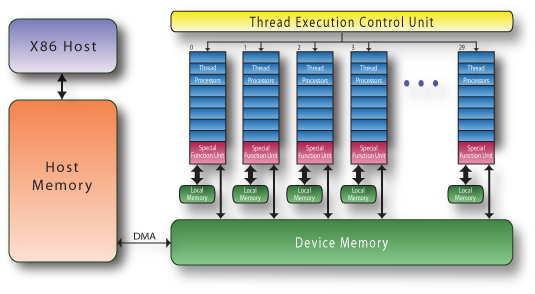
\includegraphics{09Accelerators/figures/pgi-nvidia-block-diagram.png}
\end{figure}

See
\href{http://www.gris.informatik.tu-darmstadt.de/cuda-workshop/tutorial/Advanced_CUDA_01.pdf}{more}

\subsubsection{SIMT}\label{simt}

\begin{itemize}
\itemsep1pt\parskip0pt\parsep0pt
\item
  Threads within a block have access to the same ``shared'' memory
\item
  Threads within a block can synchronise
\item
  No communication or synchronisation primitives across blocks/SMs

  \begin{itemize}
  \itemsep1pt\parskip0pt\parsep0pt
  \item
    can use atomic operations on variables in global memory (slow)
  \end{itemize}
\item
  This type of programming is a hybrid between threaded programming and
  SIMD and hence is called SIMT by Nvidia
\end{itemize}

\subsubsection{Executing code on the
GPU}\label{executing-code-on-the-gpu}

\begin{itemize}
\itemsep1pt\parskip0pt\parsep0pt
\item
  Functions executed on the GPU and called from the CPU are called
  ``kernels''

  \begin{itemize}
  \itemsep1pt\parskip0pt\parsep0pt
  \item
    kernel execution is asynchronous to the CPU
  \item
    CPU must call a function which blocks until the GPU has finished
    executing the current kernel before attempting to download results
  \item
    there is an implicit synchronisation barrier on the GPU at the start
    of each kernel
  \end{itemize}
\item
  Common programming pattern:

  \begin{itemize}
  \itemsep1pt\parskip0pt\parsep0pt
  \item
    upload data from CPU RAM to GPU global memory (slow)
  \item
    execute kernel(s) on GPU (fast)
  \item
    synchronise
  \item
    download results (slow)
  \end{itemize}
\end{itemize}

\subsubsection{GPU-accelerating your
code}\label{gpu-accelerating-your-code}

\begin{itemize}
\itemsep1pt\parskip0pt\parsep0pt
\item
  Four options to GPU accelerate code:

  \begin{itemize}
  \itemsep1pt\parskip0pt\parsep0pt
  \item
    replace existing libraries with GPU-accelerated ones
    (\href{https://arrayfire.com/}{ArrayFire},
    \href{https://developer.nvidia.com/cufft}{cuFFT},
    \href{https://developer.nvidia.com/cublas}{cuBLAS},
    \href{http://icl.cs.utk.edu/magma/}{Magma}, \ldots{})
  \item
    use compiler directives to automatically generate GPU-accelerated
    portions of code (OpenMP 4.5,
    \href{http://www.openacc.org/}{OpenACC})
  \item
    use CUDA::Thrust C++ template library to build your own kernels
  \item
    write your own kernels in CUDA-C
  \end{itemize}
\end{itemize}

\subsection{Streaming computations}\label{streaming-computations}

\subsubsection{\emph{Single Instruction}, Multiple
Data}\label{single-instruction-multiple-data}

All threads in a warp perform the exact same hardware instruction, but
on different data.

On thread 0:

\begin{Shaded}
\begin{Highlighting}[]
\NormalTok{a[}\DecValTok{0}\NormalTok{] = alpha * x[}\DecValTok{0}\NormalTok{] + }\DecValTok{1}\NormalTok{;}
\NormalTok{___syncthreads();}
\NormalTok{y[}\DecValTok{0}\NormalTok{] -= a[}\DecValTok{31}\NormalTok{];}
\end{Highlighting}
\end{Shaded}

On thread 31:

\begin{Shaded}
\begin{Highlighting}[]
\NormalTok{a[}\DecValTok{31}\NormalTok{] = alpha * x[}\DecValTok{31}\NormalTok{] + }\DecValTok{1}\NormalTok{;}
\NormalTok{__syncthreads();}
\NormalTok{y[}\DecValTok{31}\NormalTok{] -= a[}\DecValTok{0}\NormalTok{];}
\end{Highlighting}
\end{Shaded}

\subsubsection{Is this single
instruction?}\label{is-this-single-instruction}

\begin{Shaded}
\begin{Highlighting}[]
\NormalTok{a[thread_id] = ((thread_id < }\DecValTok{16}\NormalTok{) ? }\DecValTok{1}\NormalTok{: -}\DecValTok{1}\NormalTok{) + alpha * x[thread_id];}
\KeywordTok{if}\NormalTok{(thread_id < }\DecValTok{16}\NormalTok{)}
  \NormalTok{a[thread_id] = alpha * x[thread_id] + }\DecValTok{1}\NormalTok{;}
\KeywordTok{else}
  \NormalTok{a[thread_id] = alpha * x[thread_id] - }\DecValTok{1}\NormalTok{;}

\NormalTok{__syncthreads();}
\NormalTok{y[thread_id] -= a[}\DecValTok{31} \NormalTok{- thread_id];}
\end{Highlighting}
\end{Shaded}

\subsubsection{~Single Instruction, \emph{Multiple Contiguous
Data}}\label{single-instruction-multiple-contiguous-data}

Each thread in a warp should access a consecutive address in memory.
Lets create a kernel for copying a vector using a single block
consisting of a single warp (of 32 threads). Assume that the size of the
vector is a multiple of 32. \texttt{threadIdx.x} is the thread id in
Cuda, and automagically passed to each kernel.

The following is a jumble of too many expressions: put it back in order.

\begin{Shaded}
\begin{Highlighting}[]
\NormalTok{__global__ }\DataTypeTok{void} \NormalTok{copy(}\DataTypeTok{float} \NormalTok{*odata, }\DataTypeTok{const} \DataTypeTok{float} \NormalTok{*idata, }\DataTypeTok{int} \NormalTok{n)}
\NormalTok{\{}
  \NormalTok{<!-- }\KeywordTok{for} \NormalTok{(}\DataTypeTok{int} \NormalTok{j = }\DecValTok{0}\NormalTok{; }\DecValTok{32} \NormalTok{* j < n; ++j) -->}
  \NormalTok{<!-- }\KeywordTok{for} \NormalTok{(}\DataTypeTok{int} \NormalTok{j = }\DecValTok{0}\NormalTok{; }\DecValTok{32} \NormalTok{* j < n; j += }\DecValTok{32}\NormalTok{) -->}
  \NormalTok{<!-- }\KeywordTok{for} \NormalTok{(}\DataTypeTok{int} \NormalTok{j = }\DecValTok{0}\NormalTok{; j < n; ++j) -->}
  \KeywordTok{for} \NormalTok{(}\DataTypeTok{int} \NormalTok{j = }\DecValTok{0}\NormalTok{; j < n; j += }\DecValTok{32}\NormalTok{)}

  \NormalTok{odata[j + threadIdx.x] = idata[j + threadIdx.x];}
  \NormalTok{<!-- odata[j + threadIdx.x * }\DecValTok{32}\NormalTok{] = idata[j + threadIdx.x]; -->}
  \NormalTok{<!-- odata[j + threadIdx.x] = idata[j + threadIdx.x * }\DecValTok{32}\NormalTok{]; -->}
  \NormalTok{<!-- odata[j + threadIdx.x * }\DecValTok{32}\NormalTok{] = idata[j + threadIdx.x * }\DecValTok{32}\NormalTok{]; -->}
\NormalTok{\}}
\end{Highlighting}
\end{Shaded}

\subsubsection{~The joys of indexing}\label{the-joys-of-indexing}

Now imagine rewriting the same code with n by m by p blocks of threads,
where each block is u by v by w threads. You have access to the size of
the block \texttt{blockDim.x}, the index and size of the grid (of
blocks) \texttt{blockIdx.(x, y, z)} and \texttt{gridDim.(x, y, z)}.

To limit memory transfers, each warp should read and write to contiguous
arrays in memory.

See also:
\href{https://devblogs.nvidia.com/parallelforall/using-shared-memory-cuda-cc/}{shared
memory},
\href{http://cuda-programming.blogspot.co.uk/2013/02/bank-conflicts-in-shared-memory-in-cuda.html}{bank
conflicts}

\subsubsection{~Structure of Arrays or Arrays of
structures}\label{structure-of-arrays-or-arrays-of-structures}

\begin{Shaded}
\begin{Highlighting}[]
\KeywordTok{struct} \NormalTok{Atom \{ }\DataTypeTok{int} \NormalTok{x, y, z; \};}
\NormalTok{std::vector<Atom> molecule;}
\end{Highlighting}
\end{Shaded}

or

\begin{Shaded}
\begin{Highlighting}[]
\KeywordTok{struct} \NormalTok{Molecule \{}
  \NormalTok{std::vector<}\DataTypeTok{int}\NormalTok{> x;}
  \NormalTok{std::vector<}\DataTypeTok{int}\NormalTok{> y;}
  \NormalTok{std::vector<}\DataTypeTok{int}\NormalTok{> z;}
\NormalTok{\};}
\end{Highlighting}
\end{Shaded}

\subsection{Just USES}\label{just-uses}

Using Somebody Else's Software is a good way to avoid becoming a GPU
expert. But which? Check for usability and sustainability:

\begin{itemize}
\itemsep1pt\parskip0pt\parsep0pt
\item
  Does it do what you need?
\item
  What license is it under?
\item
  Is it simply available on Github/BitBucker/Gitlab?
\item
  Are there automatic tests?
\item
  Is it an active development repo? (number of commits, date of last
  commmit)
\item
  How many people/labs/companies are committing to it? (check
  pull-requests)
\item
  Is there a community of users? (check issues, wiki)
\item
  Is there documentation?
\end{itemize}

\subsubsection{Broadcasting
(Vectorization)}\label{broadcasting-vectorization}

GPU require running the \emph{same operations} over mutliple data
(SIMD). Broadcasting transforms nested loops into a set of matrix or
array operations amenable to SIMD, \emph{and} likely to be already
GPU-ized by external libraries.

Also useful for MATLAB, Python/numpy, etc\ldots{}

Example:

\[G = max(||A - R_i||)\]

for all $i$, where $A$ and $R_i$ are vectors

Naive solution with explicit loops and STL:

\begin{Shaded}
\begin{Highlighting}[]

\DataTypeTok{double} \NormalTok{naive(std::vector<std::array<}\DataTypeTok{double}\NormalTok{, }\DecValTok{3}\NormalTok{>> }\DataTypeTok{const} \NormalTok{&Rs,}
             \NormalTok{std::array<}\DataTypeTok{double}\NormalTok{, }\DecValTok{3}\NormalTok{> }\DataTypeTok{const} \NormalTok{&A) \{}
  \DataTypeTok{double} \NormalTok{result(}\DecValTok{0}\NormalTok{);}
  \KeywordTok{for}\NormalTok{(}\DataTypeTok{auto} \DataTypeTok{const} \NormalTok{&R : Rs) \{}
    \DataTypeTok{auto} \NormalTok{norm = (A[}\DecValTok{0}\NormalTok{] - R[}\DecValTok{0}\NormalTok{]) * (A[}\DecValTok{0}\NormalTok{] - R[}\DecValTok{0}\NormalTok{]) + (A[}\DecValTok{1}\NormalTok{] - R[}\DecValTok{1}\NormalTok{]) * (A[}\DecValTok{1}\NormalTok{] - R[}\DecValTok{1}\NormalTok{])}
                \NormalTok{+ (A[}\DecValTok{2}\NormalTok{] - R[}\DecValTok{2}\NormalTok{]) * (A[}\DecValTok{2}\NormalTok{] - R[}\DecValTok{2}\NormalTok{]);}
    \KeywordTok{if}\NormalTok{(result < norm)}
      \NormalTok{result = norm;}
  \NormalTok{\}}
  \KeywordTok{return} \NormalTok{std::sqrt(result);}
\NormalTok{\}}
\end{Highlighting}
\end{Shaded}

\subsubsection{Broadcasting
(Vectorization)}\label{broadcasting-vectorization-1}

\begin{enumerate}
\def\labelenumi{\arabic{enumi}.}
\itemsep1pt\parskip0pt\parsep0pt
\item
  transform A from a vector to a matrix A3xn
\item
  compute pow2 = (R - A3xn)\^{}2 elementwise
\item
  sum pow2 over columns
\item
  reduce final vector using max
\end{enumerate}

\begin{Shaded}
\begin{Highlighting}[]

\DataTypeTok{double} \NormalTok{broadcasting(std::vector<std::array<}\DataTypeTok{double}\NormalTok{, }\DecValTok{3}\NormalTok{>> }\DataTypeTok{const} \NormalTok{&Rs,}
                    \NormalTok{std::array<}\DataTypeTok{double}\NormalTok{, }\DecValTok{3}\NormalTok{> }\DataTypeTok{const} \NormalTok{&A) \{}
  \NormalTok{af::array A_3x1(A.size(), A.data());}
  \NormalTok{af::array gpuRs(A.size(), Rs.size(), Rs[}\DecValTok{0}\NormalTok{].data());}

  \DataTypeTok{auto} \DataTypeTok{const} \NormalTok{A_3xn = af::tile(A_3x1, }\DecValTok{1}\NormalTok{, Rs.size());}
  \DataTypeTok{auto} \DataTypeTok{const} \NormalTok{norms = af::sum(af::pow(gpuRs - A_3xn, }\DecValTok{2}\NormalTok{), }\DecValTok{0}\NormalTok{);}
  \DataTypeTok{auto} \DataTypeTok{const} \NormalTok{result = af::max(norms);}
  \NormalTok{std::shared_ptr<}\DataTypeTok{double}\NormalTok{> }\DataTypeTok{const} \NormalTok{host_array(result.host<}\DataTypeTok{double}\NormalTok{>(),}
                                           \NormalTok{[](}\DataTypeTok{double} \NormalTok{*ptr) \{ }\KeywordTok{delete}\NormalTok{[] ptr; \});}
  \KeywordTok{return} \NormalTok{std::sqrt(*host_array);}
\NormalTok{\}}
\end{Highlighting}
\end{Shaded}

\subsubsection{A word on transfer rate}\label{a-word-on-transfer-rate}

\begin{itemize}
\itemsep1pt\parskip0pt\parsep0pt
\item
  Transfer to GPU takes time $T_0$
\end{itemize}

\begin{Shaded}
\begin{Highlighting}[]

  \NormalTok{af::array gpuRs(A.size(), Rs.size(), Rs[}\DecValTok{0}\NormalTok{].data());}
  \NormalTok{af::array gpuA(A.size(), A.data());}
\end{Highlighting}
\end{Shaded}

\begin{itemize}
\itemsep1pt\parskip0pt\parsep0pt
\item
  Compute takes $\frac{C}{n}$, n the number of GPU threads
\end{itemize}

\begin{Shaded}
\begin{Highlighting}[]

  \DataTypeTok{auto} \DataTypeTok{const} \NormalTok{result}
      \NormalTok{= af::max(af::sum(af::pow(gpuRs - af::tile(gpuA, }\DecValTok{1}\NormalTok{, Rs.size()), }\DecValTok{2}\NormalTok{), }\DecValTok{0}\NormalTok{));}
\end{Highlighting}
\end{Shaded}

\begin{itemize}
\itemsep1pt\parskip0pt\parsep0pt
\item
  Transfer to CPU takes time $T_1$
\end{itemize}

\begin{Shaded}
\begin{Highlighting}[]

  \NormalTok{af::array gpuRs(A.size(), Rs.size(), Rs[}\DecValTok{0}\NormalTok{].data());}
  \NormalTok{af::array gpuA(A.size(), A.data());}
\end{Highlighting}
\end{Shaded}

\begin{itemize}
\itemsep1pt\parskip0pt\parsep0pt
\item
  Then, possibly $T_0 + T_1 + C/n > C$
\end{itemize}

\subsubsection{~Exercise: Broadcasting}\label{exercise-broadcasting}

\texttt{G = \textbackslash{}sum\_\{i, j, k\} cos(K\_k \textbackslash{}cdot (R\_i - R\_j))}

Given

\begin{Shaded}
\begin{Highlighting}[]
\NormalTok{std::vector<std::array<}\DataTypeTok{double}\NormalTok{, }\DecValTok{3}\NormalTok{>> }\DataTypeTok{const} \NormalTok{Rs = \{...\};}
\NormalTok{std::vector<std::array<}\DataTypeTok{double}\NormalTok{, }\DecValTok{3}\NormalTok{>> }\DataTypeTok{const} \NormalTok{Ks = \{...\};}
\end{Highlighting}
\end{Shaded}

Write code to compute G (pseudo, or real code):

\begin{enumerate}
\def\labelenumi{\arabic{enumi}.}
\itemsep1pt\parskip0pt\parsep0pt
\item
  Create an Rs array of (3, 1, n) using \texttt{af::moddims}
  (\texttt{n = Rs.size()})
\item
  Create an Rs array of (3, n, 1) using \texttt{af::moddims}
\item
  Tile appropriately
\item
  Compute the dot product using \texttt{af::moddims},
  \texttt{af::matmul}, \texttt{af::transpose}
\item
  sum over the cosine of the result
\end{enumerate}

\subsubsection{~Exercise: Line of Sight}\label{exercise-line-of-sight}

Given an n by m matrix of altitudes, with n orientations and m
distances:

\begin{Shaded}
\begin{Highlighting}[]
\NormalTok{std::vector<}\DataTypeTok{double}\NormalTok{> altitudes(nOrientations * mDistances) = \{ ... \};}
\end{Highlighting}
\end{Shaded}

Compute the whether any point i, j is in sight. A point is in sight if,
for that orientation, all previous angles between X-horizon and X-point
are smaller

\begin{verbatim}
            /---\
X---\      /     \---A
     \____/
\end{verbatim}

Angles are computed using the formula
\texttt{atan(z\_i / (stepsize * i))}.

\texttt{af::scanf} might come in handy: - given {[}a0, a1, a2, \ldots{},
aN{]} - it computes {[}0, a0, a0 + a1, a0 + a1 + a2, \ldots{}, a0 +
\ldots{} + aN{]} - leading zero is removed in exclusive scans

This function looks intrinsically difficult to parallelize, but there
are well known solutions. It is useful in many fields.

\subsection{~The end of brace wars: brainless auto
formatting}\label{the-end-of-brace-wars-brainless-auto-formatting}

Code is read more often than written:

\texttt{cpp int GCD(int a,int b) \{int r;while(b)\{r=a\%b;   a=b;b=r;\}return a;\}}

\href{https://clang.llvm.org/docs/ClangFormat.html}{clang-format} is one
possible code formatter. Add it (or any equivalent) to you editor for
automatic formating.

\subsection{Linting}\label{linting}

Software to check code for correctness:

\begin{itemize}
\itemsep1pt\parskip0pt\parsep0pt
\item
  the compilers themselves: ``-Wall''
\item
  \href{http://clang.llvm.org/extra/clang-tidy/}{clang-tidy}
\item
  \href{http://cppcheck.sourceforge.net/}{cppcheck}
\end{itemize}

example:

\texttt{cpp   if(FFTW\_plan\_flag != FFTW\_ESTIMATE \textbar{} FFTW\_PRESERVE\_INPUT) \{     ...   \}}

\subsection{Refactoring}\label{refactoring}

Once tests exist, it is easy and safe to modify the code:

Refactoring means rewriting:

\begin{itemize}
\itemsep1pt\parskip0pt\parsep0pt
\item
  to simplify existing code
\item
  to simplify future development
\item
  for legibility
\item
  to decrease tech-debt
\item
  to consolidate similar code (avoid copy-pasta)
\end{itemize}

\subsection{Checking memory allocation
intrusively}\label{checking-memory-allocation-intrusively}

There are a variety of compiler flags to check standard memory errors:

\begin{itemize}
\itemsep1pt\parskip0pt\parsep0pt
\item
  g++: \texttt{-fsanitize=address}
\item
  clang:
  \href{https://clang.llvm.org/docs/AddressSanitizer.html}{address
  sanitizer}
\end{itemize}

Good when debugging/testing, but may impact performance. May not detect
all memory errors (e.g.~read before initialization).

\subsection{Checking memory allocation
non-intrusively}\label{checking-memory-allocation-non-intrusively}

\href{http://valgrind.org/}{Valgrind} is an instrumentation framework
for Linux and (older) Mac.

It detects memory errors and leaks by intercepting every memory access,
allocation, and deallocation.

Unfortunately, Valgrind currently does not work with Mac OS/X
\textgreater{} 10.11.

So let's use docker (on Linux) and docker-machine (Windows, Mac OS/X)!

\subsection{Exercise: Traveling salesman solved by Simulated
Annealing}\label{exercise-traveling-salesman-solved-by-simulated-annealing}

Traveling Salesman Problem:

A salesman living in an n-dimensional world must visit N cities. What is
the shortest path?

Simulated Annealing:

\begin{itemize}
\itemsep1pt\parskip0pt\parsep0pt
\item
  Start from a candidate A
\item
  Create a neighbor B of A
\item
  if \texttt{path(A) \textgreater{} path(B)}, then swap A and B
\item
  else if
  \texttt{exp(beta * (path(B) - path(A))) \textgreater{} random()}, then
  swap A and B
\item
  loop until satisfied
\end{itemize}

\subsubsection{Setting up a docker VM and
docker}\label{setting-up-a-docker-vm-and-docker}

First download/update to the latest course:

\begin{verbatim}
git clone https://github.com/UCL-RITS/research-computing-with-cpp
\end{verbatim}

Creating a virtual machine is optional on Linux, and necessary on
Windows and Mac OS/X

\begin{verbatim}
> docker-machine create cpp_course  \
           --driver virtualbox      \
           --virtualbox-memory 4000 \
           --virtualbox-cpu-count 2
> eval $(docker-machine env cpp_course)
\end{verbatim}

The last lines lets docker know on which VM it should create containers.

Then ssh into the machine and look for your home directory:

\begin{verbatim}
> docker-machine ssh cpp_course
> pwd
# Mac users
> ls /Users/
# Linux users
> ls /home
# Windows users
# uhm, no idea :(, look around and let me know!
\end{verbatim}

Then, create a Dockerfile specifying the container we want:

\begin{verbatim}
> mkdir docker_dir
> cat > docker_dir/Dockerfile <<EOF
FROM ubuntu:latest
RUN  apt-get update && apt-get install -y cmake g++ valgrind
EOF
\end{verbatim}

Build an image of the container

\begin{verbatim}
> docker build -t course_container /path/to/docker_dir
\end{verbatim}

Now build the code in \texttt{11Performance/cpp} using an instance
(a.k.a container) of the image.

First, check you can see the directory with the source:

\begin{verbatim}
> docker run --rm                                               \
          -v /path/to/source/on/vm:/path/to/source/on/container \
          -w /path/to/source/on/container                       \
          course_container                                      \
          ls
\end{verbatim}

This should print the content of the directory on your machine, if:

\begin{itemize}
\itemsep1pt\parskip0pt\parsep0pt
\item
  the virtual box VM was set-up to mount your home directory (automatic)
\item
  the container was set up to mount the VM directory
  (\texttt{-v path/VM/:path/container})
\end{itemize}

Finally, replace the ls command to:

\begin{enumerate}
\def\labelenumi{\arabic{enumi}.}
\itemsep1pt\parskip0pt\parsep0pt
\item
  create a build directory in the source code directory
\item
  run cmake from the build directory
\item
  run make in the build directory
\end{enumerate}

\subsection{Running valgrind on program called
\texttt{awful}}\label{running-valgrind-on-program-called-awful}

Assuming everything went well, there should be a compiled program called
awful.

It can only run inside the container!

It has memory leaks and bugs. Investigate and correct using valgrind:

\begin{verbatim}
> docker run --rm                                         \
    -v /path/to/source/on/vm:/path/to/source/on/container \
    -w /path/to/source/on/container                       \
    course_container                                      \
    valgrind -v --leak-check=full --show-leak-kinds=all   \
                --track-origin=yes ./awful
\end{verbatim}

\subsection{Running valgrind on program called
\texttt{less\_bad}}\label{running-valgrind-on-program-called-lessux5fbad}

Even programs written without explicit memory allocations can have
memory bugs.

The next version uses Eigen to solve the same problem.

\begin{enumerate}
\def\labelenumi{\arabic{enumi}.}
\itemsep1pt\parskip0pt\parsep0pt
\item
  add \texttt{libeigen3-dev} to the Dockerfile
\item
  rebuild the image
\item
  re-build the code
\item
  run valgrind on \texttt{less\_bad}
\item
  investigate and correct the code
\end{enumerate}

\subsection{Amdahl's law}\label{amdahls-law}

Maximum theoretical speedup for parallelizing a given task.

\begin{itemize}
\item
  Given a program that takes a time T to execute
\item
  When parallelizing a task A taking time P over n threads
\item
  Then the maximum speedup is:

  $S = \frac{T}{T - P + \frac{P}{n}}$
\end{itemize}

Some simple cases:

\begin{itemize}
\itemsep1pt\parskip0pt\parsep0pt
\item
  $P \mapsto 0$, $n \mapsto \infty$, then $S \rightarrow 1$
\item
  $P=0.5$, $n \mapsto \infty$, then $S \rightarrow 2$
\end{itemize}

In practice, it means programmers/researchers should measure performance
before jumping to ``optimize'' code (a.k.a. apply the scientific
method?).

\subsection{Profiling}\label{profiling}

Refers to measuring how much time the program spends in each function:

\begin{itemize}
\itemsep1pt\parskip0pt\parsep0pt
\item
  Valgrind, via
  \href{http://valgrind.org/docs/manual/cl-manual.html}{callgrind}
  provides an accurate, non-intrusive solution
\item
  \href{https://sourceware.org/binutils/docs/gprof/}{gprof} require
  ``instrumenting'' the program, e.g.~recompiling with the gprof
  library. It polls the program every so often, a.k.a. ``sampling''
\item
  \href{{[}https://github.com/gperftools/gperftools}{gperftools},
  intrusive, thread-capable, can select parts of code to profile, info
  can be visualized by kcachegrind and/or
  \href{https://github.com/google/pprof}{pprof}
\item
  \href{https://developer.apple.com/library/content/documentation/DeveloperTools/Conceptual/InstrumentsUserGuide/}{XCode
  instruments} provides ``sampling'' without requiring instrumentation
\end{itemize}

Other considerations to take into account: threads, GPU-specifics,
MPI\ldots{}

\subsection{Exercise: Profiling the correct
\texttt{less\_bad}}\label{exercise-profiling-the-correct-lessux5fbad}

\begin{enumerate}
\def\labelenumi{\arabic{enumi}.}
\itemsep1pt\parskip0pt\parsep0pt
\item
  install \texttt{kcachegrind} or \texttt{qcachegrind} (latter on Mac +
  Homebrew, or Windows)
\item
  recompile in release mode + debug info
  \texttt{cmake -DCMAKE\_BUILD\_TYPE=RelWithDebInfo}
\item
  Run the following command:
\end{enumerate}

\begin{verbatim}
> docker run --rm \
    -v /path/to/source/on/vm:/path/to/source/on/container \
    -w /path/to/source/on/container  \
    course_container \
    valgrind -v --tool=callgrind ./awful
\end{verbatim}

\begin{enumerate}
\def\labelenumi{\arabic{enumi}.}
\itemsep1pt\parskip0pt\parsep0pt
\item
  Then run qcachegrind on the artifact file:
\end{enumerate}

\begin{verbatim}
> /usr/local/Cellar/qcachegrind/16.12.0/bin/qcachegrind callgrind.out.1
\end{verbatim}

Notice the difference between \texttt{include} and \texttt{self},
e.g.~the time spent in the function as whole, vs the time spent strictly
in the function excluding sub-function calls.

Questions:

\begin{enumerate}
\def\labelenumi{\arabic{enumi}.}
\itemsep1pt\parskip0pt\parsep0pt
\item
  How much time is spent on \texttt{neighbor}
\item
  How much time is spent on \texttt{TravelDistance::operator()}
\item
  What happens when you increase the number of cities to 100, or 10000
\item
  What should we optimize or parallelize?
\end{enumerate}

\subsection{Micro-benchmarking}\label{micro-benchmarking}

meaningful bit of code, and systematically run performance tests for
each Scientific method applied to performance: measure the time taken by
each commit.

Profiling can tell us what part to include in a benchmark.

Possible micro-benchmarking frameworks:

\begin{itemize}
\itemsep1pt\parskip0pt\parsep0pt
\item
  timers in unit test framework (not really accurate)
\item
  \href{https://github.com/google/benchmark}{google/benchmark}
\item
  \href{https://github.com/nickbruun/hayai}{hayai}, a
  ``google-test''-like framework
\item
  \href{http://www.bfilipek.com/2016/01/micro-benchmarking-libraries-for-c.html}{others}
\end{itemize}

Questions micro-benchmarking can answer:

\begin{enumerate}
\def\labelenumi{\arabic{enumi}.}
\itemsep1pt\parskip0pt\parsep0pt
\item
  How long does it take on average
\item
  Standard-deviation from average
\item
  Worst case
\end{enumerate}

Questions it doesn't always answer:

\begin{enumerate}
\def\labelenumi{\arabic{enumi}.}
\itemsep1pt\parskip0pt\parsep0pt
\item
  Performance of large subsets or whole application
\item
  Parallelization: communication vs computation
\end{enumerate}

\subsection{Exercise: build and run
\texttt{micro\_benchmark}}\label{exercise-build-and-run-microux5fbenchmark}

\texttt{micro\_benchmark} reproduces the evaluation function from the
travelling salesman problem.

It reproduces how a micro-benchmark framework works:

\begin{enumerate}
\def\labelenumi{\arabic{enumi}.}
\itemsep1pt\parskip0pt\parsep0pt
\item
  run code N times for warm-up
\item
  run code N' times for actual measurement
\end{enumerate}

Make sure the code is built in \texttt{Release} mode.

Questions:

\begin{enumerate}
\def\labelenumi{\arabic{enumi}.}
\itemsep1pt\parskip0pt\parsep0pt
\item
  Why is the float implementation faster/slower? Does the speed-up
  change with the number of dimensions or the number of cities? What
  happens for Nrow = 3?
\item
  Write a function that computes the distance manually (without Eigen
  syntactic sugar). It it faster for Nrows=2? What about Nrows=8?
\end{enumerate}

Remark:

None of these have tests (this is an exercise in bad code, after all).
Do you trust we are solving the travelling salesman problem? I
\emph{know} that \texttt{awful} does not, beyond the memory bugs\ldots{}
Because I added a bug. But maybe there are further bugs still.

How much easier would it be to test the \texttt{manual} code above if we
had tests for the evaluation function?

\section{Post-coding medley, memory leaks, and performance
measurements}\label{post-coding-medley-memory-leaks-and-performance-measurements}

\subsection{Please install docker and
docker-machine}\label{please-install-docker-and-docker-machine}

Mac OS/X:

\begin{verbatim}
> brew install Caskroom/cask/virtualbox
> brew install docker-machine
> brew install docker
\end{verbatim}

or

\begin{verbatim}
> brew install Caskroom/cask/docker-toolbox
\end{verbatim}

Linux: - docker https://www.docker.com/community-edition - docker
machine (optional): https://docs.docker.com/machine/install-machine/

Windows or Mac OS/X: - https://www.docker.com/products/docker-toolbox

\subsection{Side-note: Flynn's Taxonomy of
Parallelization}\label{side-note-flynns-taxonomy-of-parallelization}

\begin{itemize}
\itemsep1pt\parskip0pt\parsep0pt
\item
  SISD: Single instruction single data
\end{itemize}

prototypical serial code

\begin{itemize}
\itemsep1pt\parskip0pt\parsep0pt
\item
  SIMD: Single instruction multiple data
\end{itemize}

Same instruction is performed in parallel over different inputs.
Necessary in GPU (at the level of a warp of 32 threads). Likely in
OpenMP (for loop parallelization) and MPI.

\begin{itemize}
\itemsep1pt\parskip0pt\parsep0pt
\item
  MIMD: Multiple instruction multiple data
\end{itemize}

Basically, different threads or different nodes doing different things,
e.g. computing different terms in an equation, dealing one with the GUI,
the other with a database, etc\ldots{}

\begin{itemize}
\itemsep1pt\parskip0pt\parsep0pt
\item
  MISD: Multiple instructions single data
\end{itemize}

Weird\ldots{} Used for fault tolerance (different algorithm that should
lead to same output).

\subsection{All tests pass, the code works: are we done
yet?}\label{all-tests-pass-the-code-works-are-we-done-yet}

Lots of changes can be made to a code, from cosmetic to crucial:

\begin{itemize}
\itemsep1pt\parskip0pt\parsep0pt
\item
  formatting, linting, and refactoring
\item
  checking for memory leaks
\item
  profiling and performance
\item
  benchmarking
\end{itemize}

\section{Appendix - Template
Meta-Programming}\label{appendix---template-meta-programming}

\subsection{Appendix - Template
Meta-Programming}\label{appendix---template-meta-programming-1}

\subsubsection{No Longer In Course}\label{no-longer-in-course}

\begin{itemize}
\itemsep1pt\parskip0pt\parsep0pt
\item
  Notes provided \href{sec01TemplateMeta}{here} for historical reasons.
\item
  Also, read
  \href{http://erdani.com/index.php/books/modern-c-design/}{``Modern C++
  Design''}
\end{itemize}

\subsection{Template Meta-Programming
(TMP)}\label{template-meta-programming-tmp}

\subsubsection{What Is It?}\label{what-is-it-1}

\begin{itemize}
\itemsep1pt\parskip0pt\parsep0pt
\item
  See
  \href{http://en.wikipedia.org/wiki/Template_metaprogramming}{Wikipedia},
  \href{http://en.wikibooks.org/wiki/C\%2B\%2B_Programming/Templates/Template_Meta-Programming}{Wikibooks},
  \href{http://www.keithschwarz.com/talks/slides/tmp-cs242.pdf}{Keith
  Schwarz}
\item
  C++ Template

  \begin{itemize}
  \itemsep1pt\parskip0pt\parsep0pt
  \item
    Type or function, parameterised over, set of types, constants or
    functions
  \item
    Instantiated at compile time
  \end{itemize}
\item
  Meta Programme

  \begin{itemize}
  \itemsep1pt\parskip0pt\parsep0pt
  \item
    Program that produces or manipulates constructs of target language
  \item
    Typically, it generates code
  \end{itemize}
\item
  Template Meta-Programme

  \begin{itemize}
  \itemsep1pt\parskip0pt\parsep0pt
  \item
    C++ programme, uses Templates, generate C++ code at compile time
  \end{itemize}
\end{itemize}

\subsubsection{TMP is Turing Complete}\label{tmp-is-turing-complete}

\begin{itemize}
\itemsep1pt\parskip0pt\parsep0pt
\item
  Given: A \href{http://en.wikipedia.org/wiki/Turing_machine}{Turing
  Machine}

  \begin{itemize}
  \itemsep1pt\parskip0pt\parsep0pt
  \item
    Tape, head, states, program, etc.
  \end{itemize}
\item
  A language is ``Turing Complete'' if it can simulate a Turing Machine

  \begin{itemize}
  \itemsep1pt\parskip0pt\parsep0pt
  \item
    e.g.~Conditional branching, infinite looping
  \end{itemize}
\item
  Turing's work underpins much of ``what can be computed'' on a modern
  computer

  \begin{itemize}
  \itemsep1pt\parskip0pt\parsep0pt
  \item
    C, C++ no templates, C++ with templates, C++ TMP
  \item
    All Turing Complete
  \end{itemize}
\item
  Interesting that compiler can generate such theoretically powerful
  code.\\
\item
  But when, where, why, how to use TMP?\\
\item
  (side-note: Its not just a C++ pre-processor macro)
\end{itemize}

\subsubsection{Why Use It?}\label{why-use-it}

\begin{itemize}
\itemsep1pt\parskip0pt\parsep0pt
\item
  Use sparingly as code difficult to follow
\item
  Use for

  \begin{itemize}
  \itemsep1pt\parskip0pt\parsep0pt
  \item
    Optimisations
  \item
    Represent Behaviour as a Type
  \item
    Traits classes
  \end{itemize}
\item
  But when you see it, you need to understand it!
\end{itemize}

\subsubsection{Factorial Example}\label{factorial-example}

See
\href{http://en.wikipedia.org/wiki/Template_metaprogramming}{Wikipedia
Factorial Example}

\begin{itemize}
\itemsep1pt\parskip0pt\parsep0pt
\item
  This:
\end{itemize}

\begin{Shaded}
\begin{Highlighting}[]
\OtherTok{#include <iostream>}
\KeywordTok{using} \KeywordTok{namespace} \NormalTok{std;}

\KeywordTok{template} \NormalTok{<}\DataTypeTok{int} \NormalTok{n>}
\KeywordTok{struct} \NormalTok{factorial \{}
    \KeywordTok{enum} \NormalTok{\{ value = n * factorial<n - }\DecValTok{1}\NormalTok{>::value \};}
\NormalTok{\};}

\KeywordTok{template} \NormalTok{<>}
\KeywordTok{struct} \NormalTok{factorial<}\DecValTok{0}\NormalTok{> \{}
    \KeywordTok{enum} \NormalTok{\{ value = }\DecValTok{1} \NormalTok{\};}
\NormalTok{\};}

\DataTypeTok{int} \NormalTok{main () \{}
  \NormalTok{std::cout << factorial<}\DecValTok{0}\NormalTok{>::value << std::endl;}
  \NormalTok{std::cout << factorial<}\DecValTok{8}\NormalTok{>::value << std::endl;}
\NormalTok{\}}
\end{Highlighting}
\end{Shaded}

\begin{itemize}
\itemsep1pt\parskip0pt\parsep0pt
\item
  Produces:
\end{itemize}

\begin{verbatim}
1
40320
\end{verbatim}

\subsubsection{Factorial Notes:}\label{factorial-notes}

\begin{itemize}
\itemsep1pt\parskip0pt\parsep0pt
\item
  Compiler must know values at compile time

  \begin{itemize}
  \itemsep1pt\parskip0pt\parsep0pt
  \item
    i.e.~constant literal or constant expression
  \item
    See also
    \href{http://en.wikipedia.org/wiki/C\%2B\%2B11\#constexpr_.E2.80.93_Generalized_constant_expressions}{constexpr}
  \end{itemize}
\item
  Generates/Instantiates all functions recursively
\item
  Factorial 16 = 2004189184
\item
  Factorial 17 overflows
\item
  This simple example to illustrate ``computation''
\item
  But when is TMP actually useful?
\item
  Notice that parameter was an integer value \ldots{} not just ``int''
  type
\end{itemize}

\subsubsection{Loop Example}\label{loop-example}

\begin{itemize}
\itemsep1pt\parskip0pt\parsep0pt
\item
  This:
\end{itemize}

\begin{Shaded}
\begin{Highlighting}[]
\OtherTok{#include <iostream>}
\OtherTok{#include <vector>}
\KeywordTok{using} \KeywordTok{namespace} \NormalTok{std;}

\KeywordTok{template}\NormalTok{<}\KeywordTok{typename} \NormalTok{T>}
\NormalTok{T Sum(}\DataTypeTok{const} \NormalTok{std::vector<T>& data)}
\NormalTok{\{}
  \NormalTok{T total = }\DecValTok{0}\NormalTok{;}
  \KeywordTok{for} \NormalTok{(size_t i = }\DecValTok{0}\NormalTok{; i < data.size(); i++)}
  \NormalTok{\{}
    \NormalTok{total += data[i];}
  \NormalTok{\}}
  \KeywordTok{return} \NormalTok{total;}
\NormalTok{\}}

\DataTypeTok{int} \NormalTok{main () \{}
  \NormalTok{size_t numberOfInts = }\DecValTok{3}\NormalTok{;}
  \NormalTok{size_t numberOfLoops = }\DecValTok{1000000000}\NormalTok{;}
  \NormalTok{vector<}\DataTypeTok{int}\NormalTok{> a(numberOfInts);}
  \DataTypeTok{int} \NormalTok{total = }\DecValTok{0}\NormalTok{;}

  \NormalTok{std::cout << }\StringTok{"Started"} \NormalTok{<< std::endl;}
  \KeywordTok{for} \NormalTok{(size_t j = }\DecValTok{0}\NormalTok{; j < numberOfLoops; j++)}
  \NormalTok{\{}
    \KeywordTok{for} \NormalTok{(size_t i = }\DecValTok{0}\NormalTok{; i < numberOfInts; i++)}
    \NormalTok{\{}
      \NormalTok{total = Sum(a);}
    \NormalTok{\}}
  \NormalTok{\}}
  \NormalTok{std::cout << }\StringTok{"Finished:"} \NormalTok{<< total << std::endl;}
\NormalTok{\}}
\end{Highlighting}
\end{Shaded}

\begin{itemize}
\itemsep1pt\parskip0pt\parsep0pt
\item
  Time: numberOfInts=3 took 40 seconds
\end{itemize}

\subsubsection{Loop Unrolled}\label{loop-unrolled}

\begin{itemize}
\itemsep1pt\parskip0pt\parsep0pt
\item
  This:
\end{itemize}

\begin{Shaded}
\begin{Highlighting}[]
\OtherTok{#include <iostream>}
\OtherTok{#include <vector>}
\KeywordTok{using} \KeywordTok{namespace} \NormalTok{std;}

\KeywordTok{template} \NormalTok{<}\KeywordTok{typename} \NormalTok{T, }\DataTypeTok{int} \NormalTok{length>}
\KeywordTok{class} \NormalTok{FixedVector \{}
   \NormalTok{T data[length];}
  \KeywordTok{public}\NormalTok{:}
    \NormalTok{FixedVector()}
    \NormalTok{\{}
      \CommentTok{// Initialise}
      \KeywordTok{for} \NormalTok{(size_t i = }\DecValTok{0}\NormalTok{; i < length; i++)}
      \NormalTok{\{}
        \NormalTok{data[i] = }\DecValTok{0}\NormalTok{;}
      \NormalTok{\}}
    \NormalTok{\}}
    \NormalTok{T Sum()}
    \NormalTok{\{}
      \NormalTok{T sum = }\DecValTok{0}\NormalTok{;}
      \KeywordTok{for} \NormalTok{(size_t i = }\DecValTok{0}\NormalTok{; i < length; i++)}
      \NormalTok{\{}
        \NormalTok{sum += data[i];}
      \NormalTok{\}}
      \KeywordTok{return} \NormalTok{sum;}
    \NormalTok{\}}
\NormalTok{\};}

\DataTypeTok{int} \NormalTok{main () \{}
  \DataTypeTok{const} \NormalTok{size_t numberOfInts = }\DecValTok{3}\NormalTok{;}
  \DataTypeTok{const} \NormalTok{size_t numberOfLoops = }\DecValTok{1000000000}\NormalTok{;}
  \NormalTok{FixedVector<}\DataTypeTok{int}\NormalTok{, numberOfInts> a;}
  \DataTypeTok{int} \NormalTok{total = }\DecValTok{0}\NormalTok{;}

  \NormalTok{std::cout << }\StringTok{"Started"} \NormalTok{<< std::endl;}
  \KeywordTok{for} \NormalTok{(size_t j = }\DecValTok{0}\NormalTok{; j < numberOfLoops; j++)}
  \NormalTok{\{}
    \KeywordTok{for} \NormalTok{(size_t i = }\DecValTok{0}\NormalTok{; i < numberOfInts; i++)}
    \NormalTok{\{}
      \NormalTok{total = a.Sum();}
    \NormalTok{\}}
  \NormalTok{\}}
  \NormalTok{std::cout << }\StringTok{"Finished:"} \NormalTok{<< total << std::endl;}
\NormalTok{\}}
\end{Highlighting}
\end{Shaded}

\begin{itemize}
\itemsep1pt\parskip0pt\parsep0pt
\item
  Time: numberOfInts=3 took 32 seconds when switch to fixed vector, and
  23 when a raw array.
\end{itemize}

\subsubsection{Policy Checking}\label{policy-checking}

\begin{itemize}
\itemsep1pt\parskip0pt\parsep0pt
\item
  Templates parameterised by type not by behaviour
\item
  But you can make a class to represent the behaviour
\item
  See
  \href{http://www.keithschwarz.com/talks/slides/tmp-cs242.pdf}{Keith
  Schwarz} for longer example.
\end{itemize}

\subsubsection{Simple Policy Checking
Example}\label{simple-policy-checking-example}

\begin{itemize}
\itemsep1pt\parskip0pt\parsep0pt
\item
  This:
\end{itemize}

\begin{Shaded}
\begin{Highlighting}[]
\OtherTok{#include <iostream>}
\OtherTok{#include <vector>}
\OtherTok{#include <stdexcept>}

\KeywordTok{class} \NormalTok{NoRangeCheckingPolicy \{}
  \KeywordTok{public}\NormalTok{:}
    \DataTypeTok{static} \DataTypeTok{void} \NormalTok{CheckRange(size_t pos, size_t n) \{ }\KeywordTok{return}\NormalTok{; \} }\CommentTok{// no checking}
\NormalTok{\};}

\KeywordTok{class} \NormalTok{ThrowErrorRangeCheckingPolicy \{}
  \KeywordTok{public}\NormalTok{:}
    \DataTypeTok{static} \DataTypeTok{void} \NormalTok{CheckRange(size_t pos, size_t n)}
    \NormalTok{\{}
      \KeywordTok{if} \NormalTok{(pos >= n) \{ }\KeywordTok{throw} \NormalTok{std::runtime_error(}\StringTok{"Out of range!"}\NormalTok{); \}}
    \NormalTok{\}}
\NormalTok{\};}

\KeywordTok{template} \NormalTok{< }\KeywordTok{typename} \NormalTok{T}
         \NormalTok{, }\KeywordTok{typename} \NormalTok{RangeCheckingPolicy = NoRangeCheckingPolicy}
         \NormalTok{>}
\KeywordTok{class} \NormalTok{Vector}
 \NormalTok{: }\KeywordTok{public} \NormalTok{RangeCheckingPolicy}
\NormalTok{\{}

  \KeywordTok{private}\NormalTok{:}
    \NormalTok{std::vector<T> data;}
  \KeywordTok{public}\NormalTok{:}
    \CommentTok{// other methods etc.}
    \DataTypeTok{const} \NormalTok{T& }\KeywordTok{operator}\NormalTok{[] (size_t pos) }\DataTypeTok{const}
    \NormalTok{\{}
      \NormalTok{RangeCheckingPolicy::CheckRange(pos, data.size());}
      \KeywordTok{return} \NormalTok{data[pos];}
    \NormalTok{\}}
\NormalTok{\};}

\DataTypeTok{int} \NormalTok{main () \{}
  \NormalTok{Vector<}\DataTypeTok{int}\NormalTok{, ThrowErrorRangeCheckingPolicy> a;}
  \CommentTok{// a.push_back(1); or similar}
  \CommentTok{// a.push_back(2); or similar}
  \KeywordTok{try} \NormalTok{\{}
    \NormalTok{std::cout << a[}\DecValTok{3}\NormalTok{] << std::endl;}
  \NormalTok{\} }\KeywordTok{catch} \NormalTok{(}\DataTypeTok{const} \NormalTok{std::runtime_error& e)}
  \NormalTok{\{}
    \NormalTok{std::cerr << e.what();}
  \NormalTok{\}}
  \KeywordTok{return} \DecValTok{0}\NormalTok{;}
\NormalTok{\}}
\end{Highlighting}
\end{Shaded}

\begin{itemize}
\itemsep1pt\parskip0pt\parsep0pt
\item
  Produces:
\end{itemize}

\begin{verbatim}
\end{verbatim}

\subsubsection{Summary of Policy Checking
Example}\label{summary-of-policy-checking-example}

\begin{itemize}
\itemsep1pt\parskip0pt\parsep0pt
\item
  Define interface for behaviour
\item
  Parameterize over all behaviours
\item
  Use multiple-inheritance to import policies
\item
  e.g.~logging / asserts
\end{itemize}

\subsubsection{Traits}\label{traits}

\begin{itemize}
\itemsep1pt\parskip0pt\parsep0pt
\item
  From C++ standard 17.1.18

  \begin{itemize}
  \itemsep1pt\parskip0pt\parsep0pt
  \item
    ``a class that encapsulates a set of types and functions necessary
    for template classes and template functions to manipulate objects of
    types for which they are instantiated.''
  \end{itemize}
\item
  Basically: Traits represent details about a type
\item
  You may be using them already!
\item
  Start with a simple example
\end{itemize}

\subsubsection{Simple Traits Example}\label{simple-traits-example}

\begin{itemize}
\itemsep1pt\parskip0pt\parsep0pt
\item
  This:
\end{itemize}

\begin{Shaded}
\begin{Highlighting}[]
\OtherTok{#include <iostream>}

\KeywordTok{template} \NormalTok{<}\KeywordTok{typename} \NormalTok{T>}
\KeywordTok{struct} \NormalTok{is_void \{}
  \DataTypeTok{static} \DataTypeTok{const} \DataTypeTok{bool} \NormalTok{value = }\KeywordTok{false}\NormalTok{;}
\NormalTok{\};}

\KeywordTok{template} \NormalTok{<>}
\KeywordTok{struct} \NormalTok{is_void<}\DataTypeTok{void}\NormalTok{> \{}
  \DataTypeTok{static} \DataTypeTok{const} \DataTypeTok{bool} \NormalTok{value = }\KeywordTok{true}\NormalTok{;}
\NormalTok{\};}

\DataTypeTok{int} \NormalTok{main () \{}
  \NormalTok{std::cout << }\StringTok{"is_void(void)="} \NormalTok{<< is_void<}\DataTypeTok{void}\NormalTok{>::value << std::endl;}
  \NormalTok{std::cout << }\StringTok{"is_void(int)="} \NormalTok{<< is_void<}\DataTypeTok{int}\NormalTok{>::value << std::endl;}
  \KeywordTok{return} \DecValTok{0}\NormalTok{;}
\NormalTok{\}}
\end{Highlighting}
\end{Shaded}

\begin{itemize}
\itemsep1pt\parskip0pt\parsep0pt
\item
  Produces:
\end{itemize}

\begin{verbatim}
is_void(void)=1
is_void(int)=0
\end{verbatim}

\subsubsection{Traits Principles}\label{traits-principles}

\begin{itemize}
\itemsep1pt\parskip0pt\parsep0pt
\item
  Small, simple, normally public, eg. struct
\item
  else/if

  \begin{itemize}
  \itemsep1pt\parskip0pt\parsep0pt
  \item
    Else template
  \item
    partial specialisations
  \item
    full specialisations
  \end{itemize}
\item
  Probably using them already

  \begin{itemize}
  \itemsep1pt\parskip0pt\parsep0pt
  \item
    \texttt{std::numeric\_limits\textless{}double\textgreater{}::max()}
  \item
    ITK has similar
    \texttt{itk::NumericTrait\textless{}PixelType\textgreater{}}
  \end{itemize}
\item
  Applies to primatives as well as types
\end{itemize}

\subsubsection{Traits Examples}\label{traits-examples}

\begin{itemize}
\itemsep1pt\parskip0pt\parsep0pt
\item
  \href{http://blog.aaronballman.com/2011/11/a-simple-introduction-to-type-traits}{Simple
  Tutorial from Aaron Ballman}
\item
  \href{http://www.boost.org/doc/libs/?view=category_Metaprogramming}{Boost
  meta-programming support}
\item
  \href{http://www.boost.org/doc/libs/1_57_0/libs/type_traits/doc/html/boost_typetraits/background.html}{Boost
  type\_traits tutorial}
\item
  \href{http://www.cplusplus.com/reference/type_traits}{C++11 has many
  traits}
\end{itemize}

\subsubsection{Wait, Inheritance Vs
Traits?}\label{wait-inheritance-vs-traits}

\begin{itemize}
\itemsep1pt\parskip0pt\parsep0pt
\item
  We said inheritance is often overused in OO
\item
  We say that too frequent if/switch statements based on type are bad in
  OO
\item
  C++11 providing many
  \href{http://www.cplusplus.com/reference/type_traits}{is\_X type
  traits} returning bool, leading to if/else
\item
  So, when to use it?
\end{itemize}

\subsubsection{When to use Traits}\label{when-to-use-traits}

\begin{itemize}
\itemsep1pt\parskip0pt\parsep0pt
\item
  Some advice

  \begin{itemize}
  \itemsep1pt\parskip0pt\parsep0pt
  \item
    Sparingly
  \item
    To add information to templated types
  \item
    Get algorithm to work for 1 data type
  \item
    If you extend to multiple data types and consider templates

    \begin{itemize}
    \itemsep1pt\parskip0pt\parsep0pt
    \item
      When you need type specific behaviour

      \begin{itemize}
      \itemsep1pt\parskip0pt\parsep0pt
      \item
        traits probably better than template specialisation
      \item
        traits better than inheritance based template hierarchies
      \end{itemize}
    \end{itemize}
  \end{itemize}
\item
  Remember

  \begin{itemize}
  \itemsep1pt\parskip0pt\parsep0pt
  \item
    Scientist = few use-cases
  \item
    Library designer = coding for the unknown, and potentially limitless
    use-cases

    \begin{itemize}
    \itemsep1pt\parskip0pt\parsep0pt
    \item
      More likely of interest to library designers
    \end{itemize}
  \end{itemize}
\end{itemize}

\subsubsection{TMP Use in Medical Imaging -
1}\label{tmp-use-in-medical-imaging---1}

Declare an \href{http://www.itk.org}{ITK} image

\begin{Shaded}
\begin{Highlighting}[]

\KeywordTok{template}\NormalTok{< }\KeywordTok{typename} \NormalTok{TPixel, }\DataTypeTok{unsigned} \DataTypeTok{int} \NormalTok{VImageDimension = }\DecValTok{2} \NormalTok{>}
\KeywordTok{class} \NormalTok{Image:}\KeywordTok{public} \NormalTok{ImageBase< VImageDimension >}
\NormalTok{\{}
\KeywordTok{public}\NormalTok{:}
\CommentTok{// etc}
\end{Highlighting}
\end{Shaded}

\begin{itemize}
\itemsep1pt\parskip0pt\parsep0pt
\item
  TPixel, \texttt{int}, \texttt{float} etc.
\item
  VImageDimension = number of dimensions
\end{itemize}

\subsubsection{TMP Use in Medical Imaging -
2}\label{tmp-use-in-medical-imaging---2}

But what type is origin/spacing/dimensions?

\begin{Shaded}
\begin{Highlighting}[]
\KeywordTok{template}\NormalTok{< }\DataTypeTok{unsigned} \DataTypeTok{int} \NormalTok{VImageDimension = }\DecValTok{2} \NormalTok{>}
\KeywordTok{class} \NormalTok{ImageBase:}\KeywordTok{public} \NormalTok{DataObject}
\NormalTok{\{}
  \KeywordTok{typedef} \NormalTok{SpacePrecisionType                          SpacingValueType;}
  \KeywordTok{typedef} \NormalTok{Vector< SpacingValueType, VImageDimension > SpacingType;}
\end{Highlighting}
\end{Shaded}

\subsubsection{TMP Use in Medical Imaging -
3}\label{tmp-use-in-medical-imaging---3}

So now look at \texttt{Vector}

\begin{Shaded}
\begin{Highlighting}[]
\KeywordTok{template}\NormalTok{< }\KeywordTok{typename} \NormalTok{T, }\DataTypeTok{unsigned} \DataTypeTok{int} \NormalTok{NVectorDimension = }\DecValTok{3} \NormalTok{>}
\KeywordTok{class} \NormalTok{Vector:}\KeywordTok{public} \NormalTok{FixedArray< T, NVectorDimension >}
\NormalTok{\{}
\KeywordTok{public}\NormalTok{:}
\end{Highlighting}
\end{Shaded}

\subsubsection{TMP Use in Medical Imaging -
4}\label{tmp-use-in-medical-imaging---4}

Now we can see how fixed length arrays are used

\begin{Shaded}
\begin{Highlighting}[]
\KeywordTok{template}\NormalTok{< }\KeywordTok{typename} \NormalTok{T, }\DataTypeTok{unsigned} \DataTypeTok{int} \NormalTok{TVectorDimension >}
\DataTypeTok{const} \KeywordTok{typename} \NormalTok{Vector< T, TVectorDimension >::Self &}
\NormalTok{Vector< T, TVectorDimension >}
\NormalTok{::}\KeywordTok{operator}\NormalTok{+=(}\DataTypeTok{const} \NormalTok{Self & vec)}
\NormalTok{\{}
  \KeywordTok{for} \NormalTok{( }\DataTypeTok{unsigned} \DataTypeTok{int} \NormalTok{i = }\DecValTok{0}\NormalTok{; i < TVectorDimension; i++ )}
    \NormalTok{\{}
    \NormalTok{( *}\KeywordTok{this} \NormalTok{)[i] += vec[i];}
    \NormalTok{\}}
  \KeywordTok{return} \NormalTok{*}\KeywordTok{this}\NormalTok{;}
\NormalTok{\}}
\end{Highlighting}
\end{Shaded}

which may be unrolled by compiler.

\subsubsection{TMP Use in Medical Imaging -
5}\label{tmp-use-in-medical-imaging---5}

\begin{itemize}
\itemsep1pt\parskip0pt\parsep0pt
\item
  \href{http://www.itk.org}{ITK}

  \begin{itemize}
  \itemsep1pt\parskip0pt\parsep0pt
  \item
    uses
    \href{http://www.itk.org/Doxygen/html/classitk_1_1NumericTraits.html}{\texttt{itk::NumericTraits\textless{}\textgreater{}}}
    adding mathematical operators like multiplicative identity, additive
    identity
  \item
    uses traits to describe features of meshes,
    \texttt{like numeric\_limits}, but more generalised
  \end{itemize}
\item
  \href{http://www.mitk.org}{MITK} (requires coffee and a quiet room)

  \begin{itemize}
  \itemsep1pt\parskip0pt\parsep0pt
  \item
    uses
    \href{http://docs.mitk.org/2014.03/mitkPixelTypeList_8h.html}{mitkPixelTypeList.h}
    for multi-plexing across templated image to non-templated image type
  \item
    uses
    \href{http://docs.mitk.org/nightly-qt4/mitkGetClassHierarchy_8h.html}{mitkGetClassHierarchy.h}
    to extract a list of class names in the inheritance hierarchy
  \end{itemize}
\item
  \href{http://link.springer.com/chapter/10.1007\%2F978-3-319-08554-8_2}{TMP
  in B-spline based registration}:
\end{itemize}

\subsubsection{Further Reading For
Traits}\label{further-reading-for-traits}

\begin{itemize}
\itemsep1pt\parskip0pt\parsep0pt
\item
  \href{http://www.keithschwarz.com/talks/slides/tmp-cs242.pdf}{Keith
  Schwarz}
\item
  \href{http://www.cantrip.org/traits.html}{Nathan Meyers}
\item
  \href{http://www.cs.rpi.edu/~musser/design/blitz/traits.html}{Todd
  Veldhuizen, traits scientific computing}
\item
  \href{http://accu.org/index.php/journals/442}{Thaddaaeus Frogley,
  ACCU, traits tutorial}
\item
  \href{http://blog.aaronballman.com/2011/11/a-simple-introduction-to-type-traits}{Aaron
  Ballman}
\item
  \href{http://erdani.com/publications/traits.html}{Andrei Alexandrescu}
\item
  \href{http://erdani.com/publications/traits_on_steroids.html}{Andrei
  Alexandrescu traits with state}
\item
  \href{http://www.boost.org/doc/libs/?view=category_Metaprogramming}{Boost
  meta-mrogramming support}
\item
  \href{http://www.boost.org/doc/libs/1_57_0/libs/type_traits/doc/html/boost_typetraits/background.html}{Boost
  type\_traits tutorial}
\item
  \href{http://www.cplusplus.com/reference/type_traits}{C++11 has many
  traits}
\end{itemize}

\subsubsection{Further Reading In
General}\label{further-reading-in-general}

\begin{itemize}
\itemsep1pt\parskip0pt\parsep0pt
\item
  \href{http://www.amazon.co.uk/Modern-Design-Generic-Programming-Patterns/dp/0201704315/ref=sr_1_1?ie=UTF8\&qid=1421739179\&sr=8-1\&keywords=andrei+alexandrescu}{Andrei
  Alexandrescu's Book}
\item
  \href{http://herbsutter.com}{Herb Sutter}'s
  \href{http://www.gotw.ca/gotw}{Guru of The Week}, especially
  \href{http://www.gotw.ca/gotw/071.htm}{71} and
  \href{http://www.gotw.ca/publications/mxc++-item-4.htm}{this} article
\item
  And of course, keep reading
  \href{http://www.aristeia.com/books.html}{Meyers}
\end{itemize}

\subsubsection{Summary}\label{summary-4}

\begin{itemize}
\itemsep1pt\parskip0pt\parsep0pt
\item
  Learnt

  \begin{itemize}
  \itemsep1pt\parskip0pt\parsep0pt
  \item
    Notation for template function/class/meta-programming
  \item
    Uses and limitations of template function/class
  \item
    Template Meta-Programming

    \begin{itemize}
    \itemsep1pt\parskip0pt\parsep0pt
    \item
      Optimisation, loop unrolling
    \item
      Policy classes
    \item
      Traits
    \end{itemize}
  \end{itemize}
\end{itemize}

\section{Appendix - Cloud computing and big
data}\label{appendix---cloud-computing-and-big-data}

\subsection{Appendix - Cloud computing and big
data}\label{appendix---cloud-computing-and-big-data-1}

\subsubsection{No Longer In Course}\label{no-longer-in-course-1}

\begin{itemize}
\itemsep1pt\parskip0pt\parsep0pt
\item
  Notes provided \href{sec01cloud}{here} for historical reasons.
\end{itemize}

\subsubsection{Big data}\label{big-data}

Some data requires special treatment for collection, storage, and
analysis.

The `three vs':

\begin{itemize}
\itemsep1pt\parskip0pt\parsep0pt
\item
  volume
\item
  velocity
\item
  variety
\end{itemize}

\subsubsection{Cloud computing}\label{cloud-computing}

Cloud computing is an approach built around the concept of shared
resources.

\begin{itemize}
\itemsep1pt\parskip0pt\parsep0pt
\item
  dynamically add and remove computing resources as you need them.
\item
  bring up large clusters of computing power, then shut it own just as
  quickly
\end{itemize}

\subsubsection{X* as a service}\label{x-as-a-service}

Emergence of service oriented approaches:

\begin{itemize}
\itemsep1pt\parskip0pt\parsep0pt
\item
  Platform as a service (PaaS)
\item
  Software as a service (SaaS)
\item
  Infrastructure as a service (SaaS)
\end{itemize}

\subsection{Exercise 1: Working in the
cloud}\label{exercise-1-working-in-the-cloud}

\subsubsection{Spinning up an instance}\label{spinning-up-an-instance}

This example briefly run through the process of:

\begin{itemize}
\itemsep1pt\parskip0pt\parsep0pt
\item
  creating an account with a provider of cloud services
\item
  spinning up a single cloud instance using a web interface
\end{itemize}

\subsubsection{Create an account}\label{create-an-account}

A growing number of companies are offering cloud computing services, for
example:

\begin{itemize}
\itemsep1pt\parskip0pt\parsep0pt
\item
  Amazon Web Services: \url{http://aws.amazon.com}
\item
  Cloudera: \url{http://www.rackspace.co.uk/cloud}
\item
  Google Cloud Platform: \url{https://cloud.google.com}
\item
  Microsoft Azure: \url{http://azure.microsoft.com}
\end{itemize}

\subsubsection{Create a key pair}\label{create-a-key-pair}

In this exercise we will be working with Amazon Web Services.

Amazon uses public key cryptography to authenticate users, so we'll need
to create a private/public key pair:

\begin{Shaded}
\begin{Highlighting}[]
\CommentTok{# Create a key pair}
\NormalTok{$ }\KeywordTok{ssh-keygen} \NormalTok{-t rsa -f ~/.ssh/ec2 -b 4096}
\end{Highlighting}
\end{Shaded}

We then need to register our public key with Amazon Web Services.

\begin{figure}[htbp]
\centering
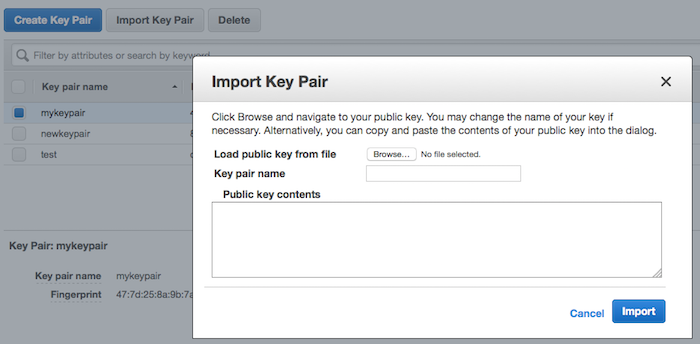
\includegraphics{97Cloud/figures/key_pair.png}
\end{figure}

\subsubsection{Create a single instance using the web
interface}\label{create-a-single-instance-using-the-web-interface}

Navigate to the EC2 Dashboard and create a `micro' instance (1 CPU,
2.5GHZ, 1GB RAM):

\begin{figure}[htbp]
\centering
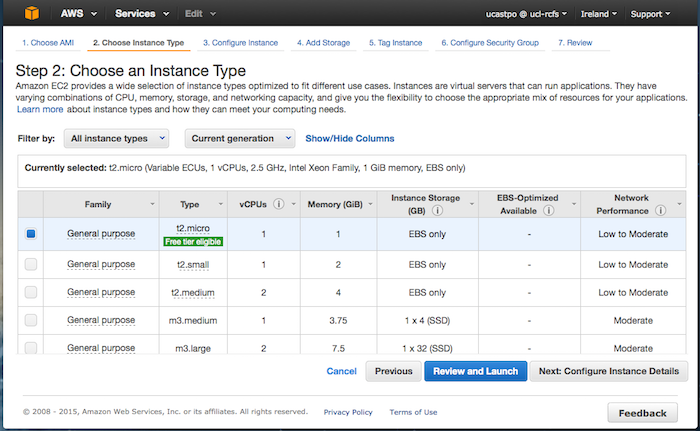
\includegraphics{97Cloud/figures/create_ec2_instance.png}
\end{figure}

\subsubsection{Connect to the instance with
SSH}\label{connect-to-the-instance-with-ssh}

For Linux instances, the username is `ec2-user':

\begin{Shaded}
\begin{Highlighting}[]
\CommentTok{# <key_file>: ~/.ssh/ec2}
\CommentTok{# <public_ID>: 52.16.106.209}
\NormalTok{$ }\KeywordTok{ssh} \NormalTok{ec2-user@}\KeywordTok{<}\NormalTok{public_ID}\KeywordTok{>} \NormalTok{-i }\KeywordTok{<}\NormalTok{key_file}\KeywordTok{>}
\end{Highlighting}
\end{Shaded}

\begin{figure}[htbp]
\centering
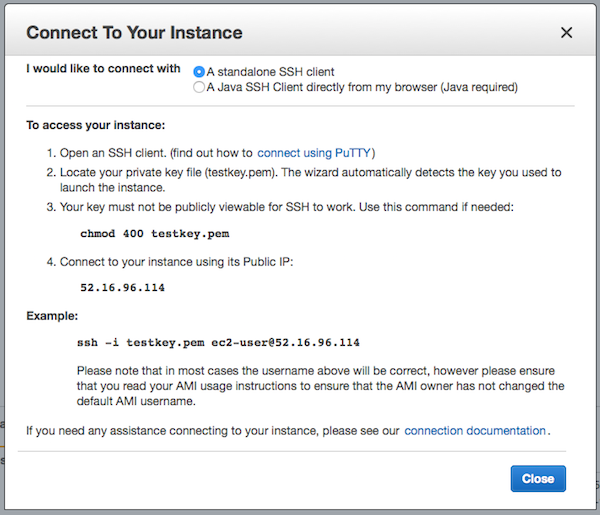
\includegraphics{97Cloud/figures/connect_to_instance.png}
\end{figure}

\begin{Shaded}
\begin{Highlighting}[]
\CommentTok{# Connected}
       \KeywordTok{__|}  \KeywordTok{__|_}  \NormalTok{)}
       \KeywordTok{_|} \DataTypeTok{\textbackslash{}(}     \KeywordTok{/}   \NormalTok{Amazon Linux AMI}
      \KeywordTok{___|}\DataTypeTok{\textbackslash{}\textbackslash{}}\KeywordTok{___|___|}

\NormalTok{[}\KeywordTok{ec2-user@ip-xxx} \NormalTok{~]$}
\end{Highlighting}
\end{Shaded}

\subsubsection{Terminate the server}\label{terminate-the-server}

When finished with the instance, remember to terminate it!

\begin{figure}[htbp]
\centering
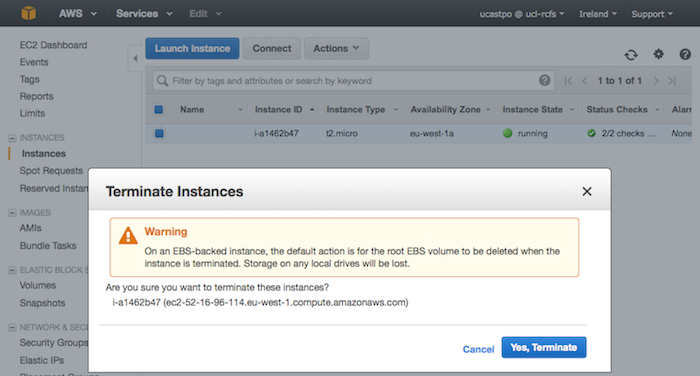
\includegraphics{97Cloud/figures/terminate_instance.png}
\end{figure}

\subsection{Exercise 2: Working in the
cloud}\label{exercise-2-working-in-the-cloud}

\subsubsection{Again, from the command
line\ldots{}}\label{again-from-the-command-line}

Install Amazon Web Services Command Line
Interface:\\\url{http://docs.aws.amazon.com/cli/latest/userguide/installing.html}

\begin{Shaded}
\begin{Highlighting}[]
\CommentTok{# install the tools with pip}
\KeywordTok{sudo} \NormalTok{pip install awscli}
\KeywordTok{aws} \NormalTok{ec2 help}
\end{Highlighting}
\end{Shaded}

\subsubsection{Configure the tools}\label{configure-the-tools}

To use the command line tools, you'll need to configure your AWS Access
Keys, region, and output
format:\\\url{http://docs.aws.amazon.com/cli/latest/userguide/cli-chap-getting-started.html}

\begin{Shaded}
\begin{Highlighting}[]
\NormalTok{$ }\KeywordTok{aws} \NormalTok{configure}

\CommentTok{# This configuration is stored locally in a home folder named .aws}
\CommentTok{# On Unix systems: ~/.aws/config;}
\CommentTok{# On Windows: %UserProfile%\textbackslash{}.aws\textbackslash{}config}
\KeywordTok{AWS} \NormalTok{Access Key ID [****************VDLA]: EXXXXXAMPLE}
\KeywordTok{AWS} \NormalTok{Secret Access Key [****************pa8o]: EXXXXXAMPLE}
\KeywordTok{Default} \NormalTok{region name [eu-west-1]: eu-west-1}
\KeywordTok{Default} \NormalTok{output format [json]: json}
\end{Highlighting}
\end{Shaded}

\subsubsection{Test our connection to Amazon Web
Services}\label{test-our-connection-to-amazon-web-services}

If our connection has been set up correctly, `describe-regions' will
return a list of Amazon Web Service regions:

\begin{Shaded}
\begin{Highlighting}[]
\CommentTok{# Successful connection will return list of AWS regions}
\CommentTok{# HTTPSConnectionPool error? Try changing region to eu-west-1}
\NormalTok{$ }\KeywordTok{aws} \NormalTok{ec2 describe-regions}
\end{Highlighting}
\end{Shaded}

\subsubsection{Create a key pair}\label{create-a-key-pair-1}

To connect to the instance, we will need a key pair. If you haven't
already done so, create one now:

\begin{Shaded}
\begin{Highlighting}[]
\CommentTok{# Create an SSH key pair}
\NormalTok{$ }\KeywordTok{ssh-keygen} \NormalTok{-t rsa -f ~/.ssh/ec2 -b 4096}
\end{Highlighting}
\end{Shaded}

Transfer the public key to AWS:

\begin{Shaded}
\begin{Highlighting}[]
\CommentTok{# <key_name> is a unique name for the pair (e.g. my-key)}
\CommentTok{# <key_blob> is the public key: "$(cat ~/.ssh/ec2.pub)"}
\NormalTok{$ }\KeywordTok{aws} \NormalTok{ec2 import-key-pair --key-name }\KeywordTok{<}\NormalTok{key_name}\KeywordTok{>} \NormalTok{\textbackslash{}}
  \KeywordTok{--public-key-material} \KeywordTok{<}\NormalTok{key_blob}\KeywordTok{>}
\end{Highlighting}
\end{Shaded}

\subsubsection{Create a security group}\label{create-a-security-group}

We'll also need to create a security group\ldots{}

\begin{Shaded}
\begin{Highlighting}[]
\CommentTok{# creates security group named my-security-group}
\NormalTok{$ }\KeywordTok{aws} \NormalTok{ec2 create-security-group \textbackslash{}}
  \KeywordTok{--group-name} \StringTok{"My security group"} \NormalTok{\textbackslash{}}
  \KeywordTok{--description} \StringTok{"SSH access from my local IP address"}
\end{Highlighting}
\end{Shaded}

\subsubsection{Configure the security
group}\label{configure-the-security-group}

\ldots{}and allow inbound connections from our local IP address:

\begin{Shaded}
\begin{Highlighting}[]
\CommentTok{# create a rule to allow inbound connections on TCP port 22}
\CommentTok{# find your IP: curl http://checkip.amazonaws.com/}
\NormalTok{$ }\KeywordTok{aws} \NormalTok{ec2 authorize-security-group-ingress \textbackslash{}}
  \KeywordTok{--group-name} \StringTok{"My security group"} \NormalTok{\textbackslash{}}
  \KeywordTok{--cidr} \KeywordTok{<}\NormalTok{local_IP_address}\KeywordTok{>}\NormalTok{/32 \textbackslash{}}
  \KeywordTok{--port} \NormalTok{22 \textbackslash{}}
  \KeywordTok{--protocol} \NormalTok{tcp}
\end{Highlighting}
\end{Shaded}

Note: the /32 at the end of the IP address is the bit number of the
\href{http://en.wikipedia.org/wiki/Classless_Inter-Domain_Routing}{CIDR
netmask}. The /32 mask is equivalent to 255.255.255.255, so defines a
single host. Lower values broaden the range of allowed addresses. An IP
of 0.0.0.0/0 would allow all inbound connections.

\subsubsection{Locate an appropriate Machine
Image}\label{locate-an-appropriate-machine-image}

An Amazon Machine Image contains the software configuration (operating
system, software\ldots{}) needed to launch an instance. AMIs are
provided by:

\begin{itemize}
\itemsep1pt\parskip0pt\parsep0pt
\item
  Amazon Web Services
\item
  the user community
\item
  AWS Marketplace
\end{itemize}

We will search for an Amazon Machine Image ID (AMI-ID) using the command
line tools:

\begin{Shaded}
\begin{Highlighting}[]
\CommentTok{# Use filter to locate a specific machine (ami-9d23aeea)}
\CommentTok{# Filter is a key,value pair}
\NormalTok{$ }\KeywordTok{aws} \NormalTok{ec2 describe-images --owners amazon \textbackslash{}}
  \KeywordTok{--filters} \StringTok{"Name=name,Values=amzn-ami-hvm-2016.09.1.20170119-x86_64-gp2"}
\end{Highlighting}
\end{Shaded}

\subsubsection{Launch an instance}\label{launch-an-instance}

Launch an instance using the Amazon Machine Image ID:

\begin{Shaded}
\begin{Highlighting}[]
\CommentTok{# <AMI-ID>: ami-70edb016}
\CommentTok{# <key_name>: defined when transferring the key}
\CommentTok{# <group_name>: "My security group"}
\NormalTok{$ }\KeywordTok{aws} \NormalTok{ec2 run-instances --image-id }\KeywordTok{<}\NormalTok{AMI-ID}\KeywordTok{>} \NormalTok{\textbackslash{}}
  \KeywordTok{--key-name} \KeywordTok{<}\NormalTok{key_name}\KeywordTok{>} \NormalTok{\textbackslash{}}
  \KeywordTok{--instance-type} \NormalTok{t2.micro \textbackslash{}}
  \KeywordTok{--security-groups} \KeywordTok{<}\NormalTok{group_name}\KeywordTok{>}
\end{Highlighting}
\end{Shaded}

\subsubsection{View the instance}\label{view-the-instance}

We can check the instance and find the public IP:

\begin{Shaded}
\begin{Highlighting}[]
\CommentTok{# View information about the EC2 instances}
\CommentTok{# e.g. state, root volume, IP address, public DNS name}
\NormalTok{$ }\KeywordTok{aws} \NormalTok{ec2 describe-instances}
\end{Highlighting}
\end{Shaded}

\subsubsection{Connect to the instance}\label{connect-to-the-instance}

Use the public IP to connect:

\begin{Shaded}
\begin{Highlighting}[]
\CommentTok{# for Linux instances, the username is ec2-user}
\CommentTok{# <public_IP>: 52.16.106.209}
\CommentTok{# <key_file>: ~/.ssh/ec2}
\NormalTok{$ }\KeywordTok{ssh} \NormalTok{-i }\KeywordTok{<}\NormalTok{key_file}\KeywordTok{>} \NormalTok{ec2-user@}\KeywordTok{<}\NormalTok{public_IP}\KeywordTok{>}
\end{Highlighting}
\end{Shaded}

You should now be connected!:

\begin{Shaded}
\begin{Highlighting}[]
\CommentTok{# Connected}
       \KeywordTok{__|}  \KeywordTok{__|_}  \NormalTok{)}
       \KeywordTok{_|} \DataTypeTok{\textbackslash{}(}     \KeywordTok{/}   \NormalTok{Amazon Linux AMI}
      \KeywordTok{___|}\DataTypeTok{\textbackslash{}\textbackslash{}}\KeywordTok{___|___|}

\NormalTok{[}\KeywordTok{ec2-user@ip-172-31-5-39} \NormalTok{~]$}
\end{Highlighting}
\end{Shaded}

\subsubsection{Terminate the instance}\label{terminate-the-instance}

Don't forget to terminate the instance when you have finished:

\begin{Shaded}
\begin{Highlighting}[]
\CommentTok{# terminate the instance}
\CommentTok{# <InstanceId>: i-87086760}
\NormalTok{$ }\KeywordTok{aws} \NormalTok{ec2 terminate-instances --instance-ids }\KeywordTok{<}\NormalTok{InstanceId}\KeywordTok{>}

\KeywordTok{TERMINATINGINSTANCES}    \NormalTok{i-87086760}
\KeywordTok{CURRENTSTATE}    \NormalTok{32  shutting-down}
\KeywordTok{PREVIOUSSTATE}   \NormalTok{16  running}
\end{Highlighting}
\end{Shaded}

\subsection{Virtualisation}\label{virtualisation}

\subsubsection{Reproducible research}\label{reproducible-research}

The ability to reproduce the analyses of research studies is
increasingly recognised as important.

Several approaches have developed that help researchers to package up
code so that their code and dependencies can be distributed and run by
others.

\subsubsection{Virtual machines}\label{virtual-machines}

A popular method for creating a shareable environment is with the use of
virtual machines.

The isolated system created by virtual machines can be beneficial, but
criticisms include:

\begin{itemize}
\itemsep1pt\parskip0pt\parsep0pt
\item
  size: virtual machines can be bulky
\item
  performance: virtual machines may use significant system resources
\end{itemize}

Tools such as Vagrant have helped to simplify the process of creating
and using virtual
machines:\\\href{https://www.vagrantup.com/}{https://www.vagrantup.com}

\subsubsection{Virtual environments}\label{virtual-environments}

Virtual environments offer an alternative to virtual machines. Rather
than constructing an entirely new system, virtual environments in
general seek to provide reproducible `containers' which are layered on
top of an existing environment.

A popular tool for creating virtual environments is
Docker:\\\href{https://www.docker.com/}{https://www.docker.com}

\subsection{Exercise 3: Virtualisation}\label{exercise-3-virtualisation}

\subsubsection{Reproducible research}\label{reproducible-research-1}

In this example, we spin up a single EC2 instance and reproduce the
analysis from a study in a virtual environment.

The simple analysis uses \texttt{countwords}, a shell script, to count
the occurrences of words in a book (in our case \texttt{dorian.txt}, The
Picture of Dorian Gray).

We will be using Docker to manage our virtual environment:
\url{https://docs.docker.com/userguide/dockerimages/}

\subsubsection{Create a new security
group}\label{create-a-new-security-group}

For this exercise we will be setting up a web connection to the EC2
instance, allowing us to connect to IPython Notebook in a browser. To
enable this connection, we will create a new security group:

\begin{Shaded}
\begin{Highlighting}[]
\NormalTok{$ }\KeywordTok{aws} \NormalTok{ec2 create-security-group --group-name }\StringTok{"ipython_notebook"} \NormalTok{\textbackslash{}}
    \KeywordTok{--description} \StringTok{"web access to ipython notebook"}
\end{Highlighting}
\end{Shaded}

We then need to configure this group to allow inbound connections:

\begin{Shaded}
\begin{Highlighting}[]
\CommentTok{# SSH}
\NormalTok{$ }\KeywordTok{aws} \NormalTok{ec2 authorize-security-group-ingress \textbackslash{}}
  \KeywordTok{--group-name} \StringTok{"ipython_notebook"} \NormalTok{\textbackslash{}}
  \KeywordTok{--cidr} \NormalTok{0.0.0.0/0 \textbackslash{}}
  \KeywordTok{--port} \NormalTok{22 \textbackslash{}}
  \KeywordTok{--protocol} \NormalTok{tcp}
\CommentTok{# port 8888}
\KeywordTok{aws} \NormalTok{ec2 authorize-security-group-ingress \textbackslash{}}
  \KeywordTok{--group-name} \StringTok{"ipython_notebook"} \NormalTok{\textbackslash{}}
  \KeywordTok{--cidr} \NormalTok{0.0.0.0/0 \textbackslash{}}
  \KeywordTok{--port} \NormalTok{8888 \textbackslash{}}
  \KeywordTok{--protocol} \NormalTok{tcp}
\end{Highlighting}
\end{Shaded}

\subsubsection{Spin up a cloud instance}\label{spin-up-a-cloud-instance}

As before, we will now spin up a new cloud instance:

\begin{Shaded}
\begin{Highlighting}[]
\CommentTok{# <AMI-ID>: e.g. ami-9d23aeea}
\CommentTok{# <key_name>: e.g. "my_key"}
\CommentTok{# <group_name>: e.g. "ipython_notebook"}
\NormalTok{$ }\KeywordTok{aws} \NormalTok{ec2 run-instances --image-id }\KeywordTok{<}\NormalTok{AMI-ID}\KeywordTok{>} \NormalTok{\textbackslash{}}
  \KeywordTok{--key-name} \KeywordTok{<}\NormalTok{key_name}\KeywordTok{>} \NormalTok{\textbackslash{}}
  \KeywordTok{--instance-type} \NormalTok{t2.micro \textbackslash{}}
  \KeywordTok{--security-groups} \KeywordTok{<}\NormalTok{group_name}\KeywordTok{>}
\end{Highlighting}
\end{Shaded}

\subsubsection{Connect with SSH}\label{connect-with-ssh}

When the instance is running, a public IP will be available:

\begin{Shaded}
\begin{Highlighting}[]
\NormalTok{$ }\KeywordTok{aws} \NormalTok{ec2 describe-instances}

\StringTok{"NetworkInterfaces"}\NormalTok{:}\KeywordTok{ [}
    \NormalTok{\{}
    \NormalTok{...}
    \StringTok{"Association"}\NormalTok{: \{}
        \StringTok{"PublicIp"}\NormalTok{: }\StringTok{"12.34.56.78"}\NormalTok{,}
        \StringTok{"PublicDnsName"}\NormalTok{: }\StringTok{"ec2-12-34-56-78.eu-west-1.compute.amazonaws.com"}
     \NormalTok{\}}
     \NormalTok{\}]}
\end{Highlighting}
\end{Shaded}

Use the public IP to connect over SSH:

\begin{Shaded}
\begin{Highlighting}[]
\CommentTok{# <key_file>: e.g. ~/.ssh/ec2}
\NormalTok{$ }\KeywordTok{ssh} \NormalTok{ec2-user@}\KeywordTok{<}\NormalTok{public_IP}\KeywordTok{>} \NormalTok{-i }\KeywordTok{<}\NormalTok{key_file}\KeywordTok{>}
\end{Highlighting}
\end{Shaded}

\subsubsection{Install and run Docker on the remote
system}\label{install-and-run-docker-on-the-remote-system}

Docker needs to be installed on the Cloud instance:

\begin{Shaded}
\begin{Highlighting}[]
\NormalTok{[}\KeywordTok{ec2-user@ip-xxx} \NormalTok{~]$ sudo yum install -y docker}
\NormalTok{[}\KeywordTok{ec2-user@ip-xxx} \NormalTok{~]$ sudo service docker start}
\end{Highlighting}
\end{Shaded}

\subsubsection{Docker environments are created by a set of
commands}\label{docker-environments-are-created-by-a-set-of-commands}

Docker environments are created by running a set of commands held within
a Dockerfile. A snippet of the Dockerfile used to create our environment
is shown below:

\begin{Shaded}
\begin{Highlighting}[]
\CommentTok{# Set the source image}
\KeywordTok{FROM} \NormalTok{ipython/scipystack:master}

\CommentTok{# Specify commands to run inside the image}
\KeywordTok{RUN} \NormalTok{apt-get update}
\KeywordTok{RUN} \NormalTok{apt-get install -y wget}

\CommentTok{# Create directory for container}
\KeywordTok{RUN} \NormalTok{mkdir /analysis}

\CommentTok{# Get the code}
\KeywordTok{ADD} \NormalTok{https://raw.githubusercontent.com/tompollard/dorian/master/mapper.py \textbackslash{}}
    \KeywordTok{~/analysis/mapper.py}

\CommentTok{# Run notebook}
\KeywordTok{RUN} \NormalTok{echo }\StringTok{"ipython notebook --ip=0.0.0.0 --port=8888 --no-browser"} \KeywordTok{>} \NormalTok{/usr/bin/notebook.sh}\KeywordTok{;} \KeywordTok{\textbackslash{}}
\KeywordTok{chmod} \NormalTok{755 /usr/bin/notebook.sh}
\KeywordTok{CMD} \NormalTok{/usr/bin/notebook.sh}

\CommentTok{# Open port to the outside world}
\KeywordTok{EXPOSE} \NormalTok{8888}
\KeywordTok{...}
\end{Highlighting}
\end{Shaded}

\subsubsection{Pull, build, and run the Docker
image}\label{pull-build-and-run-the-docker-image}

Build and run the docker environment:

\begin{Shaded}
\begin{Highlighting}[]
\CommentTok{# NB: sudo is not needed when running inside boot2docker}
\NormalTok{[}\KeywordTok{ec2-user@ip-xxx} \NormalTok{~]$ sudo docker pull tompollard/dorian:master}
\NormalTok{[}\KeywordTok{ec2-user@ip-xxx} \NormalTok{~]$ sudo docker run -t --rm=true -p 8888:8888 -i \textbackslash{}}
    \KeywordTok{tompollard}\NormalTok{/dorian:}\KeywordTok{master}
\end{Highlighting}
\end{Shaded}

IPython Notebook is now running in the virtual environment and available
to the outside environment on port 8888:

\begin{Shaded}
\begin{Highlighting}[]
\NormalTok{[}\KeywordTok{NotebookApp}\NormalTok{] Using existing profile dir: }\StringTok{'/root/.ipython/profile_default'}
\NormalTok{[}\KeywordTok{NotebookApp}\NormalTok{] Serving notebooks from local directory: /analysis}
\NormalTok{[}\KeywordTok{NotebookApp}\NormalTok{] The IPython Notebook is running at: http://0.0.0.0:8888/}
\NormalTok{[}\KeywordTok{NotebookApp}\NormalTok{] Use Control-C to stop this server and shut down all kernels (twice to skip confirmation)}\KeywordTok{.}
\KeywordTok{...}
\end{Highlighting}
\end{Shaded}

\subsubsection{Connect to the IPython
Notebook}\label{connect-to-the-ipython-notebook}

We can now connect to the IPython Notebook in a browser at the public IP
of the Amazon Instance on port 8888 (i.e.~http://\{publicIP\}:8888):

\begin{figure}[htbp]
\centering
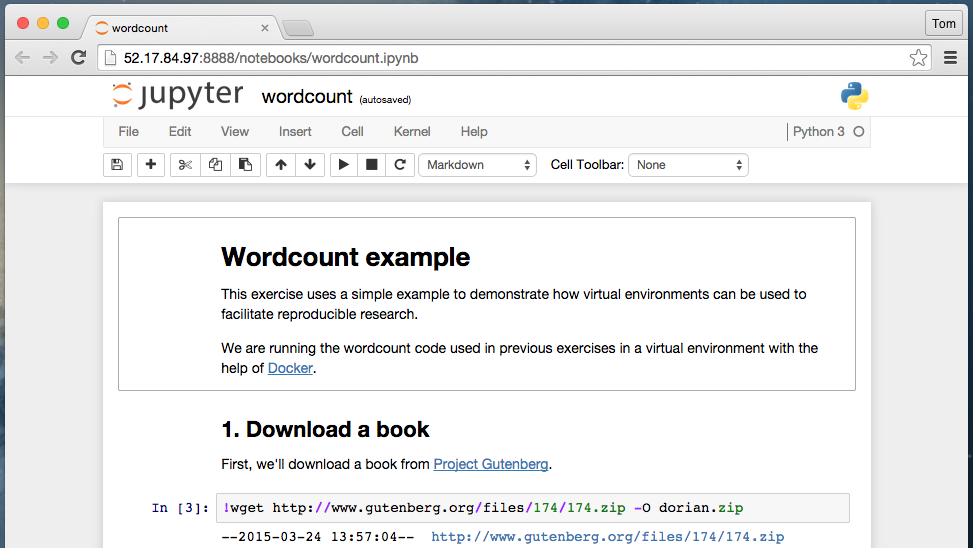
\includegraphics{97Cloud/figures/notebook.png}
\caption{IPython Notebook}
\end{figure}

\subsubsection{Now use the IPython Notebook to complete the
exercise}\label{now-use-the-ipython-notebook-to-complete-the-exercise}

Using the IPython Notebook, we can reproduce the analysis on both
existing and new datasets.

\begin{figure}[htbp]
\centering
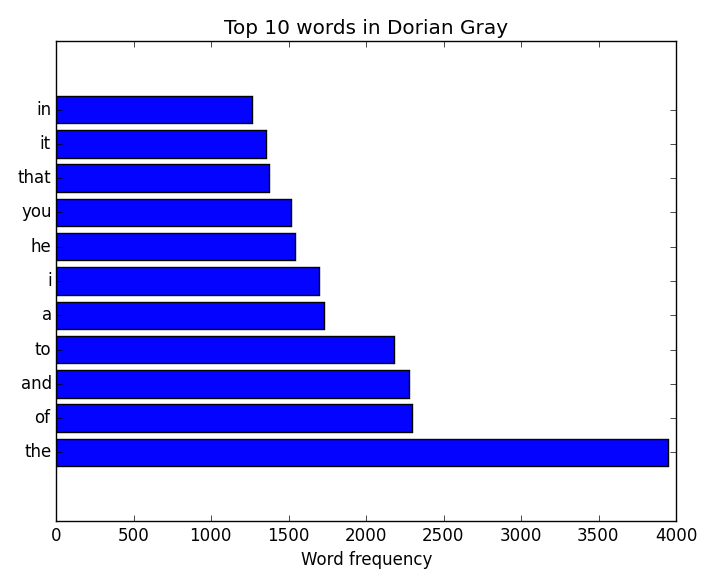
\includegraphics{97Cloud/figures/dorian_wordcount.png}
\caption{Common words in Dorian Gray}
\end{figure}

\begin{figure}[htbp]
\centering
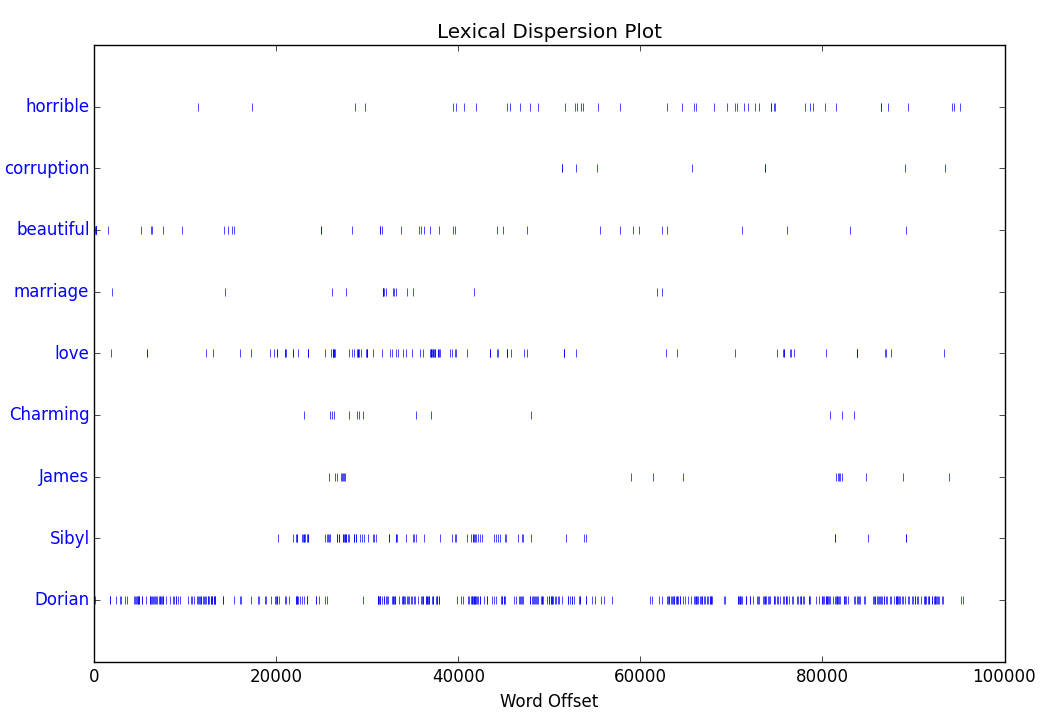
\includegraphics{97Cloud/figures/dorian_dispersion.png}
\caption{Word dispersion}
\end{figure}

\subsection{Distributed computing}\label{distributed-computing}

\subsubsection{Distributed computing}\label{distributed-computing-1}

Dividing a problem into many tasks means analysis can be shared across
multiple computers, in a parallel fashion.

Cloud computing systems have made distributed computing increasingly
accessible to individual users.

Introduced by Google in 2004, MapReduce is a popular model that supports
distributed computing on large data sets across clusters of computers.

\subsubsection{MapReduce}\label{mapreduce}

MapReduce systems are built around the concepts of:

\begin{itemize}
\itemsep1pt\parskip0pt\parsep0pt
\item
  a mapper, in which the master node takes an input, separates it into
  sub-problems, and distributes those to worker notes
\item
  a `shuffle' step to distribute data from the mapper
\item
  a reducer which collates the answers to the sub-problems and combines
  them to solves the initial question.
\end{itemize}

\subsubsection{Distributed file systems}\label{distributed-file-systems}

Distributed file systems

\begin{itemize}
\itemsep1pt\parskip0pt\parsep0pt
\item
  developed to provide reliable data storage across distributed systems
\item
  replicates data across multiple hosts to achieve reliability
\end{itemize}

\subsubsection{Hadoop}\label{hadoop}

Apache Hadoop:

\begin{itemize}
\itemsep1pt\parskip0pt\parsep0pt
\item
  framework for distributed processing of large data sets
\item
  scales from single servers to many machines
\item
  includes Hadoop MapReduce and the Hadoop Distributed File System
\end{itemize}

\subsection{Exercise 4: MapReduce}\label{exercise-4-mapreduce}

\subsubsection{The `Hello World' of
MapReduce}\label{the-hello-world-of-mapreduce}

In this example, we will demonstrate how the mapper and reducer can be
applied on our local machines to count the number of times each word
appears in a book.

\subsubsection{Choose a book}\label{choose-a-book}

Find a good book on Project Gutenberg and download it:
\url{http://www.gutenberg.org/browse/scores/top}

\begin{Shaded}
\begin{Highlighting}[]
\CommentTok{# The Picture of Dorian Gray}
\NormalTok{$ }\KeywordTok{wget} \NormalTok{http://www.gutenberg.org/cache/epub/174/pg174.txt -O dorian.txt}
\end{Highlighting}
\end{Shaded}

\begin{Shaded}
\begin{Highlighting}[]
\NormalTok{$ }\KeywordTok{head} \NormalTok{dorian.txt}

\KeywordTok{Title}\NormalTok{: The Picture of Dorian Gray}

\KeywordTok{The} \NormalTok{artist is the creator of beautiful things.  To reveal art and}
\KeywordTok{conceal} \NormalTok{the artist is art}\DataTypeTok{\textbackslash{}'}\NormalTok{s aim.  The critic is he who can translate}
\KeywordTok{into} \NormalTok{another manner or a new material his impression of beautiful}
\KeywordTok{things.}
\end{Highlighting}
\end{Shaded}

\subsubsection{Hadoop streaming}\label{hadoop-streaming}

Hadoop streaming enables MapReduce jobs to be run using any executable
as the mapper and reducer:
\url{http://hadoop.apache.org/docs/r1.2.1/streaming.html}

The mapper and reducer are written to take line-by-line inputs from
stdin and emit the output to stdout.

\subsubsection{Mapper}\label{mapper}

Our mapper:

\begin{itemize}
\itemsep1pt\parskip0pt\parsep0pt
\item
  takes lines from our book
\item
  extracts words from the line with a regular expression
\item
  outputs a tab-separated string,value pair for each word (e.g.~theword
  1)
\end{itemize}

\begin{Shaded}
\begin{Highlighting}[]
\CommentTok{#!/usr/bin/env python}
\CharTok{import} \NormalTok{sys}
\CharTok{import} \NormalTok{re}

\KeywordTok{def} \NormalTok{mapper(stream):}
    \NormalTok{pattern = re.}\DataTypeTok{compile}\NormalTok{(}\StringTok{'[a-zA-Z][a-zA-Z0-9]*'}\NormalTok{)}
    \KeywordTok{for} \NormalTok{line in stream:}
        \KeywordTok{for} \NormalTok{word in pattern.findall(line):}
            \DataTypeTok{print} \NormalTok{word.lower() + }\StringTok{'}\CharTok{\textbackslash{}t}\StringTok{'} \NormalTok{+ }\StringTok{'1'}

\NormalTok{mapper(sys.stdin)}
\end{Highlighting}
\end{Shaded}

\subsubsection{Reducer}\label{reducer}

Our reducer:

\begin{itemize}
\itemsep1pt\parskip0pt\parsep0pt
\item
  takes the word, value pairs generated by the mapper
\item
  sums the count for each word
\item
  outputs a word, count pair
\end{itemize}

\begin{Shaded}
\begin{Highlighting}[]
\CommentTok{#!/usr/bin/env python}
\CharTok{import} \NormalTok{sys}

\KeywordTok{def} \NormalTok{reducer(stream):}
    \NormalTok{mydict = \{\}}
    \NormalTok{line = stream.readline()}
    \KeywordTok{while} \NormalTok{line:}

        \CommentTok{# Get the key/value pair}
        \NormalTok{line = line.strip()}
        \NormalTok{word, count = line.split(}\StringTok{'}\CharTok{\textbackslash{}t}\StringTok{'}\NormalTok{)}
        \NormalTok{count = }\DataTypeTok{int}\NormalTok{(count)}

        \CommentTok{# Add to the dict}
        \KeywordTok{if} \NormalTok{word in mydict:}
            \NormalTok{mydict[word] += }\DecValTok{1}
        \KeywordTok{else}\NormalTok{:}
            \NormalTok{mydict[word] = }\DecValTok{1}

        \CommentTok{# Get the next line}
        \NormalTok{line = stream.readline()}

    \CommentTok{# Print the aggregated key/value pairs}
    \CommentTok{# for word in sorted(mydict.keys()): # order by word}
    \KeywordTok{for} \NormalTok{word in }\DataTypeTok{sorted}\NormalTok{(mydict, key=mydict.get, reverse=}\OtherTok{True}\NormalTok{): }\CommentTok{# or by count}
        \DataTypeTok{print} \NormalTok{word, }\StringTok{'}\CharTok{\textbackslash{}t}\StringTok{'}\NormalTok{, mydict[word]}

\NormalTok{reducer(sys.stdin)}
\end{Highlighting}
\end{Shaded}

\subsubsection{Demonstrate locally}\label{demonstrate-locally}

Download the mapper and reducer:

\begin{Shaded}
\begin{Highlighting}[]
\NormalTok{$ }\KeywordTok{git} \NormalTok{clone https://github.com/tompollard/dorian}
\end{Highlighting}
\end{Shaded}

Create a pipeline to process the book:

\begin{Shaded}
\begin{Highlighting}[]
\CommentTok{# sort represents the Hadoop shuffle}
\NormalTok{$ }\KeywordTok{cat} \NormalTok{dorian.txt }\KeywordTok{|} \KeywordTok{./mapper.py} \KeywordTok{|} \KeywordTok{./reducer.py} \KeywordTok{|} \KeywordTok{sort}

\KeywordTok{the}     \NormalTok{3948}
\KeywordTok{of}      \NormalTok{2298}
\KeywordTok{and}     \NormalTok{2279}
\KeywordTok{to}      \NormalTok{2181}
\KeywordTok{a}       \NormalTok{1730}
\KeywordTok{i}       \NormalTok{1694}
\KeywordTok{he}      \NormalTok{1544}
\KeywordTok{...}
\end{Highlighting}
\end{Shaded}

\subsection{Exercise 5: Distributed
computing}\label{exercise-5-distributed-computing}

\subsubsection{Again, with Hadoop}\label{again-with-hadoop}

In the previous exercise, we demonstrated MapReduce on our local
computer.

In this exercise we will spin up multiple cloud instances, making use of
Hadoop to carry out a distributed MapReduce operation.

We could set up multiple instances in the cloud (for example with EC2),
then configure Hadoop to run across the instances. This is not trivial
and takes time.

\subsubsection{Hadoop in the cloud}\label{hadoop-in-the-cloud}

Fortunately, several cloud providers offer configurable Hadoop services.
One such service is Amazon Elastic MapReduce (EMR).

Elastic MapReduce provides a framework for:

\begin{itemize}
\itemsep1pt\parskip0pt\parsep0pt
\item
  uploading data and code to the Simple Storage Service (S3)
\item
  analysing with a multi-instance cluster on the Elastic Compute Cloud
  (EC2)
\end{itemize}

\subsubsection{Create an S3 bucket}\label{create-an-s3-bucket}

Create an S3 bucket to hold the input data and our map/reduce functions:

\begin{enumerate}
\def\labelenumi{\arabic{enumi}.}
\itemsep1pt\parskip0pt\parsep0pt
\item
  Open the Amazon Web Services Console:
  \href{http://aws.amazon.com/}{http://aws.amazon.com}
\item
  Select ``Create Bucket'' and enter a globally unique name
\item
  Ensure the S3 Bucket shares the same region as other instances in your
  cluster
\end{enumerate}

Or, through the command line interface:

\begin{verbatim}
$ aws s3 mb s3://ucl-jh-books-example
\end{verbatim}

\subsubsection{Copy data and code to S3}\label{copy-data-and-code-to-s3}

Sample map and reduce functions are available on GitHub:

\begin{Shaded}
\begin{Highlighting}[]
\CommentTok{# clone the code from a remote repository}
\NormalTok{$ }\KeywordTok{git} \NormalTok{clone https://github.com/tompollard/dorian}
\end{Highlighting}
\end{Shaded}

Copy the data and code to S3:

\begin{Shaded}
\begin{Highlighting}[]
\CommentTok{# Copy input code and data to S3}
\CommentTok{# No support for unix-style wildcards}
\NormalTok{$ }\KeywordTok{aws} \NormalTok{s3 cp dorian.txt s3://my-bucket-ucl123/input/}
\NormalTok{$ }\KeywordTok{aws} \NormalTok{s3 cp mapper.py s3://my-bucket-ucl123/code/}
\NormalTok{$ }\KeywordTok{aws} \NormalTok{s3 cp reducer.py s3://my-bucket-ucl123/code/}
\end{Highlighting}
\end{Shaded}

\subsubsection{Launch the compute
cluster}\label{launch-the-compute-cluster}

Create a compute cluster with one master instance and two core
instances:

\begin{Shaded}
\begin{Highlighting}[]
\CommentTok{# Start a EMR cluster}
\CommentTok{# <ami-version>: version of the machine image to use}
\CommentTok{# <instance-type>:  number and type of Amazon EC2 instances}
\CommentTok{# <key_name>: "mykeypair"}
\NormalTok{$ }\KeywordTok{aws} \NormalTok{emr create-cluster --ami-version 3.11.0 \textbackslash{}}
    \KeywordTok{--ec2-attributes} \NormalTok{KeyName=student01 \textbackslash{}}
    \KeywordTok{--instance-groups} \NormalTok{InstanceGroupType=MASTER,InstanceCount=1,InstanceType=m3.xlarge \textbackslash{}}
    \OtherTok{InstanceGroupType=}\NormalTok{CORE,InstanceCount=}\KeywordTok{2}\NormalTok{,InstanceType=m3.xlarge \textbackslash{}}
    \KeywordTok{--use-default-roles}

\StringTok{"ClusterId"}\NormalTok{: }\StringTok{"j-3HGKJHEND0DX8"}
\end{Highlighting}
\end{Shaded}

\subsubsection{Get the cluster ID}\label{get-the-cluster-id}

Get the cluster-id:

\begin{Shaded}
\begin{Highlighting}[]
\CommentTok{# Get the cluster-id}
\NormalTok{$ }\KeywordTok{aws} \NormalTok{emr list-clusters}
    \KeywordTok{...}
    \StringTok{"Id"}\NormalTok{: }\StringTok{"j-3HGKJHEND0DX8"}\NormalTok{,}
    \StringTok{"Name"}\NormalTok{: }\StringTok{"Development Cluster"}
\end{Highlighting}
\end{Shaded}

\subsubsection{Get the public DNS name of the
cluster}\label{get-the-public-dns-name-of-the-cluster}

When the cluster is up and running, get the public DNS name:

\begin{Shaded}
\begin{Highlighting}[]
\CommentTok{# Get the DNS}
\NormalTok{$ }\KeywordTok{aws} \NormalTok{emr describe-cluster --cluster-id j-3HGKJHEND0DX8 \textbackslash{}}
    \KeywordTok{|} \KeywordTok{grep} \NormalTok{MasterPublicDnsName}
    \KeywordTok{...}
    \StringTok{"MasterPublicDnsName"}\NormalTok{: }\StringTok{"ec2-52-16-235-144.eu-west-1.compute.amazonaws.com"}
\end{Highlighting}
\end{Shaded}

\subsubsection{Connect to the cluster}\label{connect-to-the-cluster}

SSH into the cluster using the username `hadoop':

\begin{Shaded}
\begin{Highlighting}[]
\CommentTok{# SSH into the master node}
\CommentTok{# <key_file>: ~/.ssh/ec2}
\CommentTok{# <MasterPublicDnsName>: ec2-52-16-235-144.eu-west-1.compute.amazonaws.com}
\NormalTok{$ }\KeywordTok{ssh} \NormalTok{hadoop@}\KeywordTok{<}\NormalTok{MasterPublicDnsName}\KeywordTok{>} \NormalTok{-i }\KeywordTok{<}\NormalTok{key_file}\KeywordTok{>}
\end{Highlighting}
\end{Shaded}

\begin{Shaded}
\begin{Highlighting}[]
\CommentTok{# Connected}
       \KeywordTok{__|}  \KeywordTok{__|_}  \NormalTok{)}
       \KeywordTok{_|} \DataTypeTok{\textbackslash{}(}     \KeywordTok{/}   \NormalTok{Amazon Linux AMI}
      \KeywordTok{___|}\DataTypeTok{\textbackslash{}\textbackslash{}}\KeywordTok{___|___|}

\NormalTok{[}\KeywordTok{hadoop@ip-xxx} \NormalTok{~]$}
\end{Highlighting}
\end{Shaded}

\subsubsection{Run the analysis}\label{run-the-analysis}

\begin{Shaded}
\begin{Highlighting}[]
\CommentTok{# To process multiple input files, use a wildcard}
\NormalTok{[}\KeywordTok{hadoop@ip-xxx} \NormalTok{~]$ hadoop \textbackslash{}}
    \KeywordTok{jar} \NormalTok{contrib/streaming/hadoop-*streaming*.jar \textbackslash{}}
    \KeywordTok{-files} \NormalTok{s3://my-bucket-ucl123/code/mapper.py,s3://my-bucket-ucl123/code/reducer.py \textbackslash{}}
    \KeywordTok{-input} \NormalTok{s3://my-bucket-ucl123/input/* \textbackslash{}}
    \KeywordTok{-output} \NormalTok{s3://my-bucket-ucl123/output/ \textbackslash{}}
    \KeywordTok{-mapper} \NormalTok{mapper.py \textbackslash{}}
    \KeywordTok{-reducer} \NormalTok{reducer.py}
\end{Highlighting}
\end{Shaded}

\subsubsection{View the results}\label{view-the-results}

Results are saved to the output folder. Each reduce task writes its
output to a separate file:

\begin{Shaded}
\begin{Highlighting}[]
\CommentTok{# List files in the output folder}
\NormalTok{$ }\KeywordTok{aws} \NormalTok{s3 ls s3://my-bucket-ucl123/output/}
\end{Highlighting}
\end{Shaded}

Download the output:

\begin{Shaded}
\begin{Highlighting}[]
\CommentTok{# Copy the output files to our local folder}
\CommentTok{# No support for unix-style wildcards, so use --recursive}
\NormalTok{$ }\KeywordTok{aws} \NormalTok{s3 cp s3://my-bucket-ucl123/output . --recursive}

\CommentTok{# View the file}
\NormalTok{$ }\KeywordTok{head} \NormalTok{part-00001}

\KeywordTok{the}     \NormalTok{3948}
\KeywordTok{and}     \NormalTok{2279}
\KeywordTok{in}      \KeywordTok{1266}
\KeywordTok{his}     \NormalTok{996}
\KeywordTok{lord}    \NormalTok{248}
\KeywordTok{...}
\end{Highlighting}
\end{Shaded}

\subsubsection{Terminate the cluster}\label{terminate-the-cluster}

Once our analysis is complete, terminate the cluster:

\begin{Shaded}
\begin{Highlighting}[]
\CommentTok{# get cluster id: aws emr list-clusters}
\CommentTok{# <cluster_ID>: j-3HGKJHEND0DX8}
\NormalTok{$ }\KeywordTok{aws} \NormalTok{emr terminate-clusters --cluster-id }\KeywordTok{<}\NormalTok{cluster_ID}\KeywordTok{>}
\end{Highlighting}
\end{Shaded}

\subsubsection{Delete the bucket}\label{delete-the-bucket}

\begin{Shaded}
\begin{Highlighting}[]
\NormalTok{$ }\KeywordTok{aws} \NormalTok{s3 rb s3://my-bucket-ucl123 --force}
\end{Highlighting}
\end{Shaded}

\section{Linux Install}\label{linux-install}

\subsection{Git}\label{git-1}

If git is not already available on your machine you can try to install
it via your distribution package manager (e.g. \texttt{apt-get} or
\texttt{yum}).

On ubuntu or other Debian systems:

\begin{verbatim}
sudo apt-get install git
\end{verbatim}

On RedHat based systems:

\begin{verbatim}
sudo yum install git
\end{verbatim}

\subsection{CMake}\label{cmake-1}

Again, install the appropriate package with apt-get or yum
(\texttt{cmake}). Minimum version 3.5.

\subsection{Editor and shell}\label{editor-and-shell}

Many different text editors suitable for programming are available. If
you don't already have a favourite, you could look at
\href{http://kate-editor.org/}{Kate}.

Regardless of which editor you have chosen you should configure git to
use it. Executing something like this in a terminal should work:

\begin{verbatim}
git config --global core.editor NameofYourEditorHere
\end{verbatim}

The default shell is usually bash but if not you can get to bash by
opening a terminal and typing \texttt{bash}.

\section{Windows Install}\label{windows-install}

\subsection{Editor}\label{editor}

Unless you already use a specific editor which you are comfortable with
we recommend using
\href{http://notepad-plus-plus.org/}{\emph{Notepad++}} on windows.

Using Notepad++ to edit text files including code should be straight
forward but in addition you should configure git to use Notepad++ when
writing commit messages (see below).

\subsection{Git}\label{git-2}

Install \href{http://gitforwindows.org/}{Git for Windows}.

During the installation, you can select ``Use Notepad++ as Git's default
editor'' if you installed Notepad++ above. Make sure you tick ``Use Git
from the Windows Command Prompt'' so other Unix tools can find git. The
defaults should be suitable for other options.

Then install the \href{http://windows.github.com/}{GitHub for Windows
client}.

\subsection{CMake}\label{cmake-2}

Install
\href{http://www.cmake.org/cmake/resources/software.html}{cmake}.
Minimum version 3.5.

And choose to add it to the path for all users if so prompted. (You may
need to log out and log back in again before this takes effect!)

\subsection{Unix tools}\label{unix-tools}

Install \href{http://sourceforge.net/projects/mingw/}{MinGW} by
following the download link. It should install MinGW's package manager.
On the left, select \texttt{Basic Setup}, and on the right select
\texttt{mingw32-base}, \texttt{mingw-developer-toolkit,}
\texttt{mingw-gcc-g++} and \texttt{msys-base}. On some systems these
package might be selected from start. Finally, click the installation
menu and \texttt{Apply Changes}.

\subsection{Locating your install}\label{locating-your-install}

Now, we need to find out where Git and Notepad++ have been installed,
this will be either in \texttt{C:\textbackslash{}Program Files (x86)} or
in \texttt{C:\textbackslash{}Program Files}. The former is the norm on
more modern versions of windows. If you have the older version, replace
\texttt{Program\textbackslash{} Files\textbackslash{} \textbackslash{}(x86\textbackslash{})}
with \texttt{Program\textbackslash{} Files} in the instructions below.

\subsection{Telling Shell where to find the
tools}\label{telling-shell-where-to-find-the-tools}

We need to tell the new shell installed by MinGW where Notepad++ is.

To do this, use NotePad++ to edit the file at
\texttt{C:\textbackslash{}MinGW\textbackslash{}mysys\textbackslash{}1.0\textbackslash{}etc\textbackslash{}profile}

and toward the end, above the line \texttt{alias clear=clsb} add the
following:

\begin{Shaded}
\begin{Highlighting}[]
\CommentTok{# Path settings from SoftwareCarpentry}
\KeywordTok{export} \OtherTok{PATH=$PATH}\NormalTok{:/c/Program}\DataTypeTok{\textbackslash{} }\NormalTok{Files}\DataTypeTok{\textbackslash{} \textbackslash{}(}\NormalTok{x86}\DataTypeTok{\textbackslash{})}\NormalTok{/Notepad++}
\CommentTok{# End of Software carpentry settings}
\end{Highlighting}
\end{Shaded}

\subsection{Finding your terminal}\label{finding-your-terminal}

Check this works by opening MinGW shell, with the start menu
(Start-\textgreater{}All
programs-\textgreater{}MinGW-\textgreater{}MinGW Shell). This should
open a \emph{terminal} window, where commands can be typed in directly.

On windows 8 and 10, there may be no app for MinGW. In that case, open
the \texttt{run} app and type in

\begin{Shaded}
\begin{Highlighting}[]
\KeywordTok{C}\NormalTok{:\textbackslash{}MinGW\textbackslash{}msys\textbackslash{}1.0\textbackslash{}msys.bat}
\end{Highlighting}
\end{Shaded}

You can also create a shortcut to this file on your Desktop for quicker
access.

\subsection{Checking which tools you
have}\label{checking-which-tools-you-have}

Once you have a terminal open, type

\begin{Shaded}
\begin{Highlighting}[]
\KeywordTok{which} \NormalTok{notepad++}
\end{Highlighting}
\end{Shaded}

which should produce readout similar to

\begin{verbatim}
/c/Program Files (x86)/Notepad++/notepad++.exe
\end{verbatim}

Also try:

\begin{Shaded}
\begin{Highlighting}[]
\KeywordTok{which} \NormalTok{git}
\end{Highlighting}
\end{Shaded}

which should produce

\begin{verbatim}
/c/Program Files/Git/cmd/git.exe
\end{verbatim}

The \texttt{which} command is used to figure out where a given program
is located on disk.

\subsection{Tell Git about your
editor}\label{tell-git-about-your-editor}

If you didn't do this as part of the Git install, you now need to update
the default editor used by Git.

\begin{Shaded}
\begin{Highlighting}[]
\KeywordTok{git} \NormalTok{config --global core.editor }\StringTok{"'C:/Program Files (x86)/Notepad++}
\StringTok{    /notepad++.exe' -multiInst  -nosession -noPlugin"}
\end{Highlighting}
\end{Shaded}

Note that it is not obvious how to copy and paste text in a Windows
terminal including Git Bash. Copy and paste can be found by right
clicking on the top bar of the window and selecting the commands from
the drop down menu (in a sub menu).

You should now have a working version of git and notepad++, accessible
from your shell.

\section{Mac Install}\label{mac-install}

\subsection{XCode and command line
tools}\label{xcode-and-command-line-tools}

Install \href{https://itunes.apple.com/us/app/xcode/id497799835}{XCode}
using the Mac app store.

Then, go to Xcode\ldots{}Preferences\ldots{}Downloads\ldots{} and
install the command line tools option

\subsection{Git}\label{git-3}

Install Homebrew via typing this at a terminal:

\begin{Shaded}
\begin{Highlighting}[]
\KeywordTok{ruby} \NormalTok{-e }\StringTok{"}\OtherTok{$(}\KeywordTok{curl} \NormalTok{-fsSL https://raw.github.com/mxcl/homebrew/go}\OtherTok{)}\StringTok{"}
\end{Highlighting}
\end{Shaded}

and then type

\begin{Shaded}
\begin{Highlighting}[]
\KeywordTok{brew} \NormalTok{install git}
\end{Highlighting}
\end{Shaded}

Then install the \href{http://mac.github.com}{GitHub for Mac client}.
(If you have problems with older versions of OSX, it's safe to skip
this.)

\subsection{CMake}\label{cmake-3}

Just do

\begin{Shaded}
\begin{Highlighting}[]
\KeywordTok{brew} \NormalTok{install cmake}
\end{Highlighting}
\end{Shaded}

Minimum version 3.5.

\subsection{Editor and shell}\label{editor-and-shell-1}

The default text editor on OS X \emph{textedit} should be sufficient for
our use. Alternatively choose from a
\href{http://mac.appstorm.net/roundups/office-roundups/top-10-mac-text-editors/}{list}
of other good editors.

To setup git to use \emph{textedit} executing the following in a
terminal should do.

\begin{Shaded}
\begin{Highlighting}[]
\KeywordTok{git} \NormalTok{config --global core.editor}
    \KeywordTok{/Applications/TextEdit.app/Contents/MacOS/TextEdit}
\end{Highlighting}
\end{Shaded}

The default terminal on OSX should also be sufficient. If you want a
more advanced terminal \href{http://www.iterm2.com/}{iTerm2} is an
alternative.

\section{Installing Boost}\label{installing-boost}

\subsection{Linux Users}\label{linux-users}

Install the appropriate package with apt-get or yum, for example:

\begin{Shaded}
\begin{Highlighting}[]
\KeywordTok{sudo} \NormalTok{apt-get install boost}
\end{Highlighting}
\end{Shaded}

On Ubuntu 13.04 boost is spilt into multiple packages. The package
needed here is ``libboost1.53-dev'' and to install it you should do:

\begin{Shaded}
\begin{Highlighting}[]
\KeywordTok{sudo} \NormalTok{apt-get install libboost1.53-dev}
\end{Highlighting}
\end{Shaded}

Check that your package manager is delivering at least version 1.53, if
you have an earlier version, you will need to download from source,
following the windows instructions below.

\subsection{Mac Users}\label{mac-users}

\begin{Shaded}
\begin{Highlighting}[]
\KeywordTok{brew} \NormalTok{install boost}
\end{Highlighting}
\end{Shaded}

\subsection{Windows Users}\label{windows-users}

You will need to download and install boost manually.

Create an appropriate folder, somewhere near your working code for the
course.

For example, if you are working in
\texttt{/home/myusername/devel/cppcourse/rsd-cppcourse/reactor} you
could do:

\begin{Shaded}
\begin{Highlighting}[]
\KeywordTok{mkdir} \NormalTok{-p ~/devel/libraries/boost}
\KeywordTok{cd} \NormalTok{~/devel/libraries/boost}
\end{Highlighting}
\end{Shaded}

Now, download and unzip boost, which will take quite a while:

\begin{Shaded}
\begin{Highlighting}[]
\KeywordTok{curl} \NormalTok{-L http://sourceforge.net/projects/boost/files/...}
        \KeywordTok{...boost/1.54.0/boost_1_54_0.zip/download} \KeywordTok{>} \NormalTok{boost.zip}
\KeywordTok{unzip} \NormalTok{boost.zip}
\end{Highlighting}
\end{Shaded}

(All one line, not literally two lines with dots!)

\subsection{CMake and Boost}\label{cmake-and-boost}

If we download from source, before we next build, we will need to tell
our shell where the boost library can be found

\begin{Shaded}
\begin{Highlighting}[]
\KeywordTok{cd} \NormalTok{build}
\KeywordTok{export} \OtherTok{CMAKE_INCLUDE_PATH=}\NormalTok{/home/myusername/devel/libraries/boost_1_54_0}
\KeywordTok{cmake} \NormalTok{..}
\KeywordTok{make}
\KeywordTok{ctest}
\end{Highlighting}
\end{Shaded}

\ldots{} or your equivalent.

\section{Installation}\label{installation}

\subsection{Installation Instructions}\label{installation-instructions}

\subsubsection{Introduction}\label{introduction-5}

This document contains instructions for installation of the packages
we'll be using during the course. You will be following the training on
your own machines, so please complete these instructions. You don't need
everything before lecture one: you can refer to these instructions as
the course proceeds.

\subsubsection{What you'll need by the end of the
course}\label{what-youll-need-by-the-end-of-the-course}

\begin{itemize}
\itemsep1pt\parskip0pt\parsep0pt
\item
  \href{http://www.cmake.org}{CMake} build tool.
\item
  \href{https://github.com/philsquared/Catch}{Catch} unit testing
  framework.
\item
  \href{https://git-scm.com/}{Git} and the
  \href{https://github.com/}{GitHub} website.
\item
  Some C++ libraries: The Boost C++ library package, and ITK, the
  Insight Toolkit
\item
  An SSH Client for remote access with an SSH keypair
\item
  Fabric remote server access scripting library for Python.
\item
  X client
\item
  A code editor of your choice.
\end{itemize}

\subsubsection{Eduroam}\label{eduroam}

We will be using UCL's
\href{http://www.ucl.ac.uk/isd/staff/wireless/eduroam}{eduroam} service
to connect to the internet for this work.

So you should ensure you have eduroam installed and working.

\subsection{Assignment 2}\label{assignment-2}

\subsubsection{Serial Solution}\label{serial-solution}

Build a C++ implementation of Conway's Game of Life. See for example
https://en.wikipedia.org/wiki/Conway\%27s\_Game\_of\_Life {[}5 Marks{]}

Marks Scheme:

\begin{itemize}
\itemsep1pt\parskip0pt\parsep0pt
\item
  Valid code: 1 mark.
\item
  Readable code: 1 marks.
\item
  Appropriate unit tests: 1 marks.
\item
  Well-structured project layout and build system: 1 mark.
\item
  Use of version control: 1 mark.
\end{itemize}

\subsubsection{Organising remote
computation}\label{organising-remote-computation}

Define an appropriate output file format, and use a script in a dynamic
language (Python, MATLAB, R, Ruby, Perl etc) to create an mpeg video of
your results. Use a script to deploy your serial code on a remote
cluster with qsub. {[}5 marks{]}

Marks scheme:

\begin{itemize}
\itemsep1pt\parskip0pt\parsep0pt
\item
  Output file works: 1 mark.
\item
  Visualiser works: 1 mark.
\item
  Automated deployment script with fabric or bash: 1 mark.
\item
  Output file and script organisation support reproducible research: 1
  mark.
\item
  Valid job submission script: 1 mark.
\end{itemize}

\subsubsection{Shared memory
parallelism}\label{shared-memory-parallelism-2}

Parallelise your code using OpenMP. Create a graph of performance versus
core count on a machine with at least 12 cores. Comment on your
findings. {[}5 Marks{]}

Marks scheme:

\begin{itemize}
\itemsep1pt\parskip0pt\parsep0pt
\item
  Valid OpenMP parallelisation: 1 mark.
\item
  Preprocessor usage so that code remains valid without OpenMP: 1 mark
\item
  Script to organise job runs and results for performance measurement: 1
  mark.
\item
  Clear and meaningful scaling graph: 1 mark.
\item
  Discussion: 1 mark
\end{itemize}

\subsubsection{Distributed memory
parallelism}\label{distributed-memory-parallelism-2}

Parallelise your code using MPI, with a 2-dimensional spatial
decomposition scheme. Create a performance graph with at least 12 cores.
Comment on your findings. {[}5 marks{]}

Marks scheme:

\begin{itemize}
\itemsep1pt\parskip0pt\parsep0pt
\item
  Valid MPI parallelisation: 1 mark.
\item
  Valid 2-dimensional decomposition scheme: 1 mark.
\item
  Unit tests to exercise decomposition sheme: 1 mark.
\item
  Performance graph, with script to organise measurement runs and clear
  graph: 1 mark
\item
  Discussion: 1 mark
\end{itemize}

\subsubsection{Accelerators}\label{accelerators-1}

Accelerate your serial solution using at least one of CUDA Thrust, CUDA
C or OpenCL. Experiment with different thread counts and performance
optimisations. Measure speedup compared to the serial code, either on a
cluster or using a graphics card on your own computer. Comment on your
findings. (There is one mark available for a second accelerator
solution.) {[}5 marks{]}

Marks scheme:

\begin{itemize}
\itemsep1pt\parskip0pt\parsep0pt
\item
  Valid accelerator parallelisation: 1 mark
\item
  Clean, readable, tested code: 1 mark
\item
  Optimisation by exploring different thread counts and other
  configurable parameters: 1 mark
\item
  Speedup analysis and discussion: 1 mark
\item
  Second accelerator parallelisation: 1 mark.
\end{itemize}

\subsubsection{Submission of the
assignment}\label{submission-of-the-assignment}

You should submit your solution via Moodle, including the entire code
repository with version control history. Your solution should include a
text report with a discussion of your project and a clear explanation of
how to build and invoke your code -- the marker will deduct marks if the
code cannot easily be built and run as indicated. Your report should be
broken down into sections that reflect those of the assignment, and
should include your graphs, performance measurements, and discussion of
any problems or interesting design decisions you encounter along the
way. You should separate your solutions for each section with version
control revision numbers, tags or branches and describe these in the
report.

\section{Assessment}\label{assessment}

\subsection{Assessment Structure}\label{assessment-structure}

\begin{itemize}
\itemsep1pt\parskip0pt\parsep0pt
\item
  3 hour exam

  \begin{itemize}
  \itemsep1pt\parskip0pt\parsep0pt
  \item
    Past papers from 2015 and later are available, but syllabus does
    evolve
  \item
    Past marks schemes and standard solutions are not available
  \end{itemize}
\item
  2 pieces coursework - 40 hours each

  \begin{itemize}
  \itemsep1pt\parskip0pt\parsep0pt
  \item
    1 due 3rd week March
  \item
    1 due just after Easter
  \end{itemize}
\end{itemize}
